% 150 câu đã gỡ khỏi ngân hàng (chuyen_dang) — chép lại vào file dạng để khôi phục

% từ: cau-hoi/lop10/0D6_Thong_ke/0D6-4-4_Phuong_sai_do_lech_chuan_cua_mau_so_lieu.tex
\begin{bt}%[0D6V4-4][V]%[BG10-3in1, Phạm Ngọc Trung]%[ma:1a9ec396]
	Biểu đồ sau ghi lại nhiệt độ lúc $12$ giờ trưa tại một trạm quan trắc trong $10$ ngày liên tiếp (đơn vị: $^\circ\mathrm{C}$):
	\begin{center}
		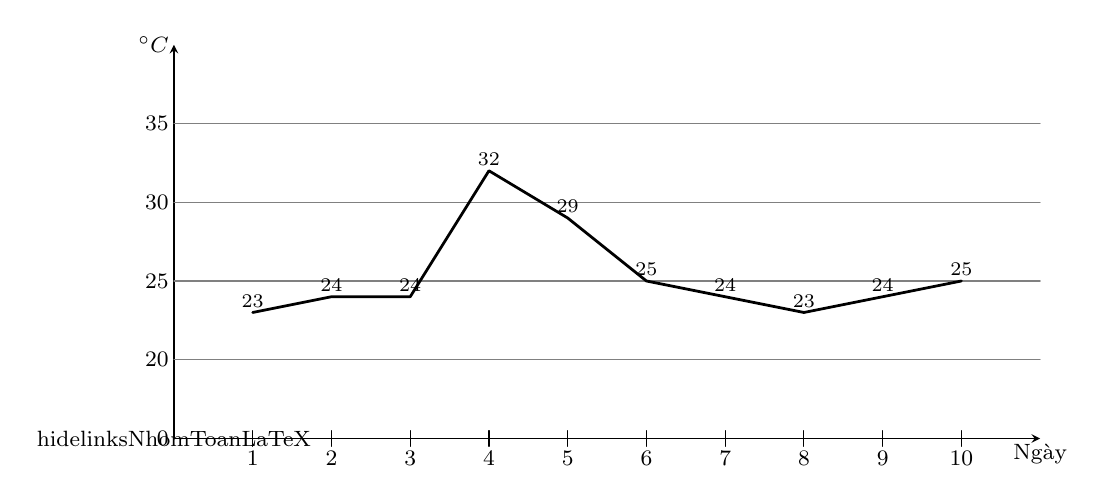
\begin{tikzpicture}[font=\footnotesize, line join=round, line cap=round, >=stealth, scale=1]
			\draw[->] (0,0)--(0,5)node[left]{$^\circ\text{C}$};
			\draw[->] (0,0)--(11,0) node[below]{Ngày};
			\foreach \x/\y in {0/0,1/20,2/25,3/30,4/35} {
				\draw (0,\x) node[left]{$\y$};}
			\foreach \x in {1,2,3,4,5,6,7,8,9,10}\draw (\x,0.1)--(\x,-0.1) node [below] {\footnotesize $\x$};
			\path (0,0) node{\hypersetup{hidelinks}\href{NhomToanLaTeX}{ }};
			\foreach \x in {1,2,...,4} { \draw[gray] (0,\x)--(11,\x); }
			\draw [line width=1pt] (1,1.6)node[above]{\scriptsize $23$}--(2,1.8)node[above]{\scriptsize $24$}--(3,1.8)node[above]{\scriptsize $24$}--(4,3.4)node[above]{\scriptsize $32$}--(5,2.8)node[above]{\scriptsize $29$}--(6,2)node[above]{\scriptsize $25$}--(7,1.8)node[above]{\scriptsize $24$}--(8,1.6)node[above]{\scriptsize $23$}--(9,1.8)node[above]{\scriptsize $24$}--(10,2)node[above]{\scriptsize $25$};
		\end{tikzpicture}
	\end{center}
	Phương sai của mẫu số liệu bằng bao nhiêu (làm tròn kết quả đến hàng phần trăm)?
	
	\shortans[]{7{,}61} 
	\loigiai{
		Từ biểu đồ đã cho ta có bảng số liệu thống kê
		\begin{center}
			{\setlength\extrarowheight{2pt}
				\begin{tabular}{|>{\centering\arraybackslash}m{2cm}|*{5}{>{\centering\arraybackslash}m{1cm}|}}
					\hline 
					Giá trị &$23$&$24$&$25$&$29$&$32$ \\
					\hline 
					Tần số &$2$&$4$&$2$&$1$&$1$ \\ 
					\hline
			\end{tabular}}
		\end{center}
		Nhiệt độ trung bình của mẫu số liệu là 
		\allowdisplaybreaks
		\begin{eqnarray*}
			\overline{x}=\dfrac{23\cdot2+24\cdot4+25\cdot2+29\cdot1+32\cdot1}{10}=25{,}3.
		\end{eqnarray*} 
		Phương sai của mẫu số liệu trên là 
		\allowdisplaybreaks
		\begin{eqnarray*}
			s^2=\dfrac{2\cdot(23-\overline{x})^2 +4\cdot(24-\overline{x})^2 +2\cdot(25-\overline{x})^2 +1\cdot(29-\overline{x})^2 +1\cdot(32-\overline{x})^2}{10}=7{,}61.
		\end{eqnarray*}
	} 
\end{bt}

% từ: cau-hoi/lop10/0D7_Bat_phuong_trinh_bac_2_mot_an/0D7-1-3_Bai_toan_xet_dau_biet_BXD_do_thi.tex
\begin{bt}%[0D7H1-3]%[0K6KG-2]%[ma:08a7106d]
	\immini{Dựa vào đồ thị của hàm số bậc hai $y=f(x)$ ở hình bên, hãy
	\begin{enumerate}
		\item Lập bảng xét dấu của tam thức bậc hai đã cho.
		\item Giải bất phương trình $f(x)\ge 0$.
	\end{enumerate}}{\begin{tikzpicture}[>=stealth,scale=1, line join=round, line cap=round]
	%\def\a{1} \def\b{-4} \def\c{3} % Hệ số
	\def\xmin{-1.5} \def\xmax{2.6} \def\ymin{-2.5} \def\ymax{1.2}
	%	\draw[line width=0.1pt,dashed] (\xmin,\ymin) grid (\xmax,\ymax);
	\draw[->] (\xmin,0)--(\xmax,0) node [below]{$x$};
	\draw[->] (0,\ymin)--(0,\ymax) node [left]{$y$};
	\node at (0,0) [above left]{$O$};
	\draw[fill=black] (1/3,0) circle (1pt) node[above]{$\frac{1}{3}$};
	\clip (\xmin+0.1,\ymin+0.1) rectangle (\xmax-0.5,\ymax-0.1);
	\draw[smooth,samples=300] plot(\x,{-(\x-1/3)^2});
\end{tikzpicture}}
\loigiai{
	\begin{enumerate}
		\item Dựa vào đồ thị, ta có bảng xét dấu như sau:
		\begin{center}
			
\begin{tikzpicture}
				\tkzTabInit[nocadre=false,lgt=2,espcl=2.1]
				{$x$ /0.6,$f(x)$ /0.6}
				{$-\infty$,$\frac{1}{3}$,$+\infty$}
				\tkzTabLine{,-,$0$,-,}
			\end{tikzpicture}
		\end{center}
	\item Dựa vào đồ thị, ta có $f(x)\geq 0\Leftrightarrow x=\dfrac{1}{3}$.\\
	Tập nghiệm của bất phương trình là $S=\left\{\dfrac{1}{3}\right\}$.
	\end{enumerate}
}
\end{bt}

% từ: cau-hoi/lop10/0D7_Bat_phuong_trinh_bac_2_mot_an/0D7-2-1_Bat_phuong_trinh_bac_2_va_ung_dung.tex
\begin{ex}%[0D7N2-1]%[ma:ee71e9d4]
	Xét dấu tam thức $f(x)=-3x^2+2x+8$. Khẳng  định nào sau đây đúng?
	 \choice
		 {\True $f(x) \geq 0$ khi $x \in\left[-\dfrac{4}{3}; 2\right]$}
		{$f(x) \leq 0$ khi  $x \in\left(-\infty;-\dfrac{4}{3}\right) \cup[2;+\infty)$}
		{$f(x) \leq 0$ khi  $x \in\left(-\dfrac{4}{3}; 2\right)$}
		{$f(x) \geq 0$ khi $x \in\left(-\dfrac{4}{3};  2\right)$}
	\loigiai{ 
		Ta  có $-3x^2+2x+8=0\Leftrightarrow\hoac{&x=2\\
		&x=-\dfrac{4}{3}.}$\\ 
		Bảng xét dấu 
		\begin{center}
			
\begin{tikzpicture}[scale=0.8,font=\footnotesize,line join=round,line cap=round,>=stealth]
					\tkzTabInit[lgt=3] 
						{$x$/1.5,$f (x)$/1} 
						 {$-\infty$,$-\dfrac{4}{3}$,$2$,$+\infty$}
					 \tkzTabLine{,-,0,+,0,-,}
				\end{tikzpicture}
		\end{center}
		Khẳng  định $f(x) \geq 0$ khi $x \in\left[-\dfrac{4}{3}; 2\right]$.\\
		$f(x) \leq 0$ khi  $x \in\left(-\infty;-\dfrac{4}{3}\right]\cup \left[2;+\infty \right) $.
	} 
\end{ex}

% từ: cau-hoi/lop10/0D7_Bat_phuong_trinh_bac_2_mot_an/0D7-2-6_Bai_toan_co_tham_so.tex
\begin{bt}%[0D7N2-6]%[Dự án đề kiểm tra HKII NH22-23-Thy Nguyen Vo Diem]%[Bình Phú]%[ma:a4d2f471]
\begin{enumerate}
	\item Lập bảng xét dấu tam thức $f(x)=-x^2+5 x-6$.
	\item Cho $g(x)=m x^2-2 m x-2$. Xác định $m$ để $g(x) \leq 0$,  $\forall x \in  \mathbb{R}$.
	\item Cho $h(x)=x^2\left(9-x^2\right)$. Xác định số nguyên $a$ lớn nhất thỏa $h(a)>0$.
\end{enumerate}
\loigiai{
\begin{enumerate}
	\item Cho $f(x)=0 \Leftrightarrow \hoac{&x=3\\&x=2}$. Do $a=-1<0$ nên ta có bảng xét dấu $f(x)$
	\begin{center}

\begin{tikzpicture}
\tkzTabInit[lgt=1.2,espcl=3]
{$x$ /0.7, $f(x)$ /0.7}
{$-\infty$,$2$,$3$,$+\infty$}
\tkzTabLine{ ,-,0,+,0,-, }
\end{tikzpicture}
\end{center}
	\item \textbf{TH1:} $m=0$, ta có $g(x)=-2 \le 0$, $\forall x \in \mathbb{R}$. Vậy $m=0$ thỏa đề.\\
	\textbf{TH2:} $m \ne 0$.
	\allowdisplaybreaks{\begin{eqnarray*}
		g(x) \leq 0, \, \forall x \in \mathbb{R}	&\Leftrightarrow& m x^2-2 m x-2 \leq 0, \, \forall x \in \mathbb{R} \\
			&\Leftrightarrow& \heva{&\Delta'\le0\\&a<0} \\
			&\Leftrightarrow& \heva{&m^2+2m\le0\\&m<0} \\
			&\Leftrightarrow& \heva{&-2 \le m \le 0\\&m<0}\\
			&\Leftrightarrow& -2 \le m < 0.
	\end{eqnarray*}}
Kết hợp điều kiện $m \ne 0$, ta có $-2 \le m < 0$.\\
Vậy $-2 \le m \le 0$ thỏa yêu cầu bài toán.
	\item Xét $h(x)=x^2\left(9-x^2\right)$ có $x^2 \ge 0$, $\forall x \in \mathbb{R}$ nên 
	\[h(x)>0	\Leftrightarrow \heva{&x \ne 0\\& 9-x^2>0} \Leftrightarrow \heva{&x \ne 0\\& -3<x<3} \Leftrightarrow \hoac{&-3<x<0\\&0<x<3}.\]
	Vậy số nguyên $a$ lớn nhất thỏa $h(a)>0$ là $a=2$.
\end{enumerate}
}
\end{bt}

% từ: cau-hoi/lop10/0D8_Dai_so_to_hop/0D8-3-2_Khai_trien_mot_nhi_thuc_Newton.tex
\begin{ex}%[0D8H3-2]%[ma:0e260e3f]
	Viết khai triển theo công thức nhị thức  Newtơn $(x-y)^5$.
	 \choice
		{\True  $x^5-5x^4y+10x^3y^2-10x^2y^3+5xy^4-y^5$}
		{$x^5+5x^4y+10x^3y^2+10x^2y^3+5xy^4+y^5$} 
		{$x^5-5x^4y-10x^3y^2-10x^2y^3-5xy^4+y^5$} 
		 {$x^5+5x^4y-10x^3y^2+10x^2y^3-5xy^4+y^5$}
	 \loigiai{
		$\begin{aligned}
		\text{Ta có  }
		 (x-y)^5&=\mathrm{C}_5^0x^5+\mathrm{C}_5^1x^4(-y)+\mathrm{C}_5^2x^3(-y)^2+\mathrm{C}_5^3x^2(-y)^3+\mathrm{C}_5^4x(-y)^4+\mathrm{C}_5^5(-y)^5 \\
		 &=x^5-5x^4y+10x^3y^2-10x^2y^3+5xy^4-y^5.
	\end{aligned}$
} 
\end{ex}

% từ: cau-hoi/lop10/0H4_He_thuc_luong_trong_tam_giac/0H4-1-2_Tinh_cac_gia_tri_luong_giac.tex
\begin{bt}%[0H4N1-2]%[Đỗ Minh Phúc]%[ma:9d39b260]
	Trên nửa đường tròn đơn vị, cho góc $\alpha$ như hình vẽ. Hãy chỉ ra các giá trị lượng giác của góc $\alpha$.
	\begin{center}
		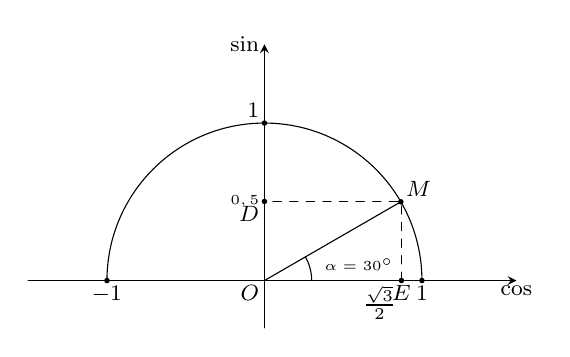
\begin{tikzpicture}[scale=1, font=\footnotesize,line join=round, line cap=round, >=stealth,x=2cm,y=2cm]
			\def\x{.87} %x0
			\def\a{30} % goc alpha
			\pgfmathsetmacro{\y}{\x*tan(\a)}
			\draw[->] (-1.5,0)--(1.6,0) node [below]{$\cos$};
			\draw[->] (0,-0.3)--(0,1.5) node [left]{$\sin$};
			\node at (0,0) [below left]{$O$};
			\draw (1,0) arc (0:180:2cm);
			\fill (1,0) node[below]{$1$} circle(1pt);
			\fill (-1,0) node[below]{$-1$} circle(1pt);
			\fill (0,1) node[above left]{$1$} circle(1pt);
			\fill (\x,0) node[below left]{$\frac{\sqrt{3}}{2}$} circle(1pt);
			\fill (\x,0) node[below]{$E$};
			\fill (\a:1) node[above right]{$M$} circle(1pt);
			\fill (0,\y) node[below left]{$D$} circle(1pt);
			\fill (0,\y) node[left]{\tiny$0,5$};
			\draw[dashed] (\x,0)|-(0,\y);
			\draw (0,0)--(\a:1); %OM
			\draw (0.3,0) arc (0:\a:0.6cm);
			\node at (.6,.1){\tiny $\alpha=30^\circ$};
		\end{tikzpicture}
	\end{center}
	\loigiai{
		Ta có
		$$\sin \alpha=\overline{OD}=0{,}5; \cos \alpha=\overline{OE}=\dfrac{\sqrt{3}}{2}; \tan \alpha=\dfrac{\sin \alpha}{\cos \alpha}=\dfrac{\overline{OD}}{\overline{OE}}=\dfrac{\sqrt{3}}{3}; \cot \alpha=\dfrac{\cos \alpha}{\sin \alpha}=\dfrac{\overline{OE}}{\overline{OD}}=\sqrt{3}.$$
	}
\end{bt}

% từ: cau-hoi/lop10/0H4_He_thuc_luong_trong_tam_giac/0H4-1-2_Tinh_cac_gia_tri_luong_giac.tex
\begin{bt}%[0H4N1-2]%[Đỗ Minh Phúc]%[ma:1e37ce33]
	Trên nửa đường tròn đơn vị, cho góc $\alpha$ như hình vẽ. Hãy chỉ ra các giá trị lượng giác của góc $\alpha$.
	\begin{center}
		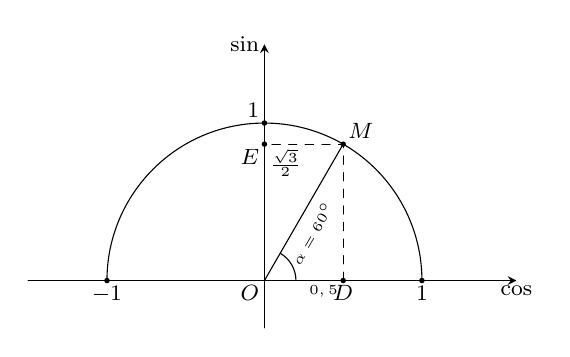
\begin{tikzpicture}[scale=1, font=\footnotesize,line join=round, line cap=round, >=stealth,x=2cm,y=2cm]
			\def\x{0.5} %x0
			\def\a{60} % goc alpha
			\pgfmathsetmacro{\y}{\x*tan(\a)}
			\draw[->] (-1.5,0)--(1.6,0) node [below]{$\cos$};
			\draw[->] (0,-0.3)--(0,1.5) node [left]{$\sin$};
			\node at (0,0) [below left]{$O$};
			\draw (1,0) arc (0:180:2cm);
			\fill (1,0) node[below]{$1$} circle(1pt);
			\fill (-1,0) node[below]{$-1$} circle(1pt);
			\fill (0,1) node[above left]{$1$} circle(1pt);
			\fill (\x,0) node[below left]{\tiny$0,5$} circle(1pt);
			\fill (\x,0) node[below]{$D$};
			\fill (\a:1) node[above right]{$M$} circle(1pt);
			\fill (0,\y) node[below left]{$E$} circle(1pt);
			\fill (0,\y) node[below right]{\tiny$\frac{\sqrt{3}}{2}$};
			\draw[dashed] (\x,0)|-(0,\y);
			\draw (0,0)--(\a:1); %OM
			\draw (0.2,0) arc (0:\a:0.4cm);
			\node[rotate=60] at (.3,.3){\tiny $\alpha=60^\circ$};
		\end{tikzpicture}
	\end{center}    
	\loigiai{
		Ta có
		$$\sin \alpha=\overline{OE}=\dfrac{\sqrt{3}}{2}; \cos \alpha=\overline{OD}=0{,}5; \tan \alpha=\dfrac{\sin \alpha}{\cos \alpha}=\dfrac{\overline{OE}}{\overline{OD}}=\sqrt{3}; \cot \alpha=\dfrac{\cos \alpha}{\sin \alpha}=\dfrac{\overline{OD}}{\overline{OE}}=\dfrac{\sqrt{3}}{3}.$$
	}
\end{bt}

% từ: cau-hoi/lop10/0H4_He_thuc_luong_trong_tam_giac/0H4-1-2_Tinh_cac_gia_tri_luong_giac.tex
\begin{bt}%[0H4N1-2]%[Đỗ Minh Phúc]%[ma:51e1ccff]
	Trên nửa đường tròn đơn vị, cho góc $\alpha$ như hình vẽ. Hãy chỉ ra các giá trị lượng giác của góc $\alpha$.
	\begin{center}
		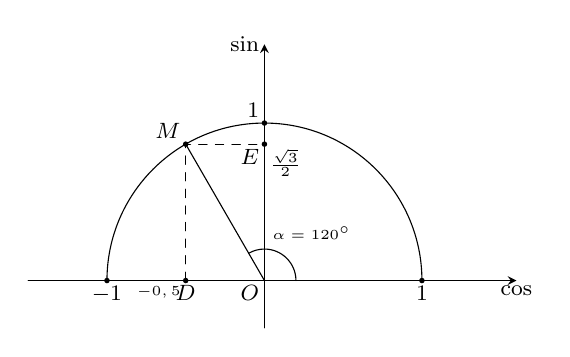
\begin{tikzpicture}[scale=1, font=\footnotesize,line join=round, line cap=round, >=stealth,x=2cm,y=2cm]
			\def\x{-0.5} %x0
			\def\a{120} % goc alpha
			\pgfmathsetmacro{\y}{\x*tan(\a)}
			\draw[->] (-1.5,0)--(1.6,0) node [below]{$\cos$};
			\draw[->] (0,-0.3)--(0,1.5) node [left]{$\sin$};
			\node at (0,0) [below left]{$O$};
			\draw (1,0) arc (0:180:2cm);
			\fill (1,0) node[below]{$1$} circle(1pt);
			\fill (-1,0) node[below]{$-1$} circle(1pt);
			\fill (0,1) node[above left]{$1$} circle(1pt);
			\fill (\x,0) node[below left]{\tiny$-0,5$} circle(1pt);
			\fill (\x,0) node[below]{$D$};
			\fill (\a:1) node[above left]{$M$} circle(1pt);
			\fill (0,\y) node[below left]{$E$} circle(1pt);
			\fill (0,\y) node[below right]{\tiny$\frac{\sqrt{3}}{2}$};
			\draw[dashed] (\x,0)|-(0,\y);
			\draw (0,0)--(\a:1); %OM
			\draw (0.2,0) arc (0:\a:0.4cm);
			\node at (.3,.3){\tiny $\alpha=120^\circ$};
		\end{tikzpicture}
	\end{center}    
	\loigiai{
		Ta có $$\sin \alpha=\overline{OE}=\dfrac{\sqrt{3}}{2}; \cos \alpha=\overline{OD}=-0{,}5; \tan \alpha=\dfrac{\sin \alpha}{\cos \alpha}=\dfrac{\overline{OE}}{\overline{OD}}=-\sqrt{3}; \cot \alpha=\dfrac{\cos \alpha}{\sin \alpha}=\dfrac{\overline{OD}}{\overline{OE}}=-\dfrac{\sqrt{3}}{3}.$$
	}
\end{bt}

% từ: cau-hoi/lop10/0H4_He_thuc_luong_trong_tam_giac/0H4-1-2_Tinh_cac_gia_tri_luong_giac.tex
\begin{bt}%[0H4N1-2]%[Đỗ Minh Phúc]%[ma:cfb04b7e]
	Trên nửa đường tròn đơn vị, cho góc $\alpha$ như hình vẽ. Hãy chỉ ra các giá trị lượng giác của góc $\alpha$.
	\begin{center}
		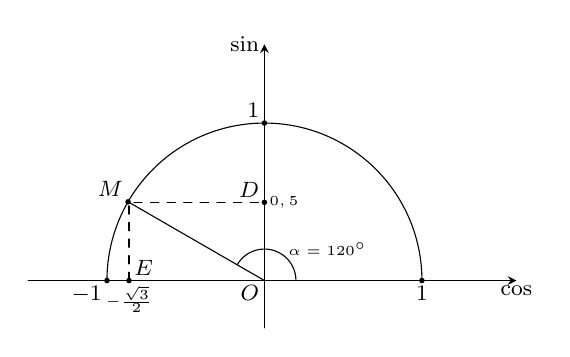
\begin{tikzpicture}[scale=1, font=\footnotesize,line join=round, line cap=round, >=stealth,x=2cm,y=2cm]
			\def\x{-0.86} %x0
			\def\a{150} % goc alpha
			\pgfmathsetmacro{\y}{\x*tan(\a)}
			\draw[->] (-1.5,0)--(1.6,0) node [below]{$\cos$};
			\draw[->] (0,-0.3)--(0,1.5) node [left]{$\sin$};
			\node at (0,0) [below left]{$O$};
			\draw (1,0) arc (0:180:2cm);
			\fill (1,0) node[below]{$1$} circle(1pt);
			\fill (-1,0) node[below left]{$-1$} circle(1pt);
			\fill (0,1) node[above left]{$1$} circle(1pt);
			\fill (\x,0) node[below]{\tiny$-\frac{\sqrt{3}}{2}$} circle(1pt);
			\fill (\x,0) node[above right]{$E$};
			\fill (\a:1) node[above left]{$M$} circle(1pt);
			\fill (0,\y) node[above left]{$D$} circle(1pt);
			\fill (0,\y) node[right]{\tiny$0,5$};
			\draw[dashed] (\x,0)|-(0,\y);
			\draw (0,0)--(\a:1); %OM
			\draw (0.2,0) arc (0:\a:0.4cm);
			\node at (.4,.2){\tiny $\alpha=120^\circ$};
		\end{tikzpicture}
	\end{center}    
	\loigiai{
		Ta có
		$$\sin \alpha=\overline{OD}=0{,}5; \cos \alpha=\overline{OE}=-\dfrac{\sqrt{3}}{2}; \tan \alpha=\dfrac{\sin \alpha}{\cos \alpha}=\dfrac{\overline{OD}}{\overline{OE}}=-\dfrac{\sqrt{3}}{3}; \cot \alpha=\dfrac{\cos \alpha}{\sin \alpha}=\dfrac{\overline{OE}}{\overline{OD}}=-\sqrt{3}.$$
	}
\end{bt}

% từ: cau-hoi/lop10/0H4_He_thuc_luong_trong_tam_giac/0H4-1-2_Tinh_cac_gia_tri_luong_giac.tex
\begin{bt}%[0H4H1-2]%[Dự án 4 - TLDH - TeamTeXHoa - Huỳnh Đức Vũ]%%[ma:7a07c6b4]
	Tính giá trị các biểu thức sau
	\begin{enumerate}
		\item $A=\sin^23^\circ+\sin^215^\circ+\sin^275^\circ+\sin^287^\circ$.
		\item  $B=\cos{0^\circ}+\cos{20^\circ}+\cos{40^\circ}+\ldots +\cos{160^\circ}+\cos{180^\circ}$.
		\item $C=\tan{5^\circ}\cdot\tan{10^\circ}\cdot\tan{15^\circ}\cdot \tan{80^\circ}\cdot\tan{85^\circ}$.
	\end{enumerate}
	\loigiai{
		\begin{enumerate}
			\item Ta có 
			\allowdisplaybreaks
			\begin{eqnarray*}
				A&=&\left(\sin^23^\circ+\sin^287^\circ\right)+\left(\sin^215^\circ+\sin^275^\circ\right)\\
				&=&\left(\sin^23^\circ+\cos^23^\circ\right)+\left(\sin^215^\circ+\cos^215^\circ\right)\\ 
				&=&1+1=2.
			\end{eqnarray*}
			\item Ta có 
			\allowdisplaybreaks
			\begin{eqnarray*}
				B&=&\left(\cos{0^\circ}+\cos{180^\circ}\right)+\left(\cos{20^\circ}+\cos{160^\circ}\right)+\ldots +\left(\cos{80^\circ}+\cos{100^\circ}\right)\\
				&=&\left(\cos{0^\circ}-\cos{0^\circ}\right)+\left(\cos{20^\circ}-\cos{20^\circ}\right)+\ldots +\left(\cos{80^\circ}-\cos{80^\circ}\right)\\ 
				&=&0. 
			\end{eqnarray*}
			\item  Ta có 
			\allowdisplaybreaks
			\begin{eqnarray*}
				C&=&\left(\tan{5^\circ}\cdot\tan{85^\circ}\right)\cdot\left(\tan{15^\circ}\cdot\tan{75^\circ}\right)\cdot \left(\tan{45^\circ}\cdot\tan{45^\circ}\right)\\
				&=&\left(\tan{5^\circ}\cdot\cot{5^\circ}\right)\cdot\left(\tan{15^\circ}\cdot\cot{15^\circ}\right)\cdot \left(\tan{45^\circ}\cdot\cot{45^\circ}\right)\\ 
				&=&1.
			\end{eqnarray*}
	\end{enumerate}}
\end{bt}

% từ: cau-hoi/lop10/0H4_He_thuc_luong_trong_tam_giac/0H4-1-3_Bien_doi_rut_gon_bieu_thuc_luong_giac.tex
\begin{bt}%[0H4V1-3]%[ma:9644951a]
	Tính giá trị biểu thức  $P=\sqrt{\sin^{4}x+6\cos^{2}x+3\cos^{4}x}+\sqrt{\cos^{4}x+6\sin^{2}x+3\sin^{4}x}$
	 \loigiai{
		Ta có $\sin^{4}x = (1-\cos^{2}x)^{2} = 1-2\cos^{2}x+\cos^{4}x$.\\ 
		$P_1  = \sin^{4}x+6\cos^{2}x+3\cos^{4}x = (1-2\cos^{2}x+\cos^{4}x)+6\cos^{2}x+3\cos^{4}x = 4\cos^{4}x+4\cos^{2}x+1 \\P_1= (2\cos^{2}x+1)^{2}$.\\
		$P_2 = \cos^{4}x+6\sin^{2}x+3\sin^{4}x = (1-2\sin^{2}x+\sin^{4}x)+6\sin^{2}x+3\sin^{4}x = 4\sin^{4}x+4\sin^{2}x+1 \\P_2=  (2\sin^{2}x+1)^{2}$.\\
		$P=\sqrt{(2\cos^{2}x+1)^{2}}+\sqrt{(2\sin^{2}x+1)^{2}}$.\\ 
		Vì $2\cos^{2}x+1>0$ và $2\sin^{2}x+1>0$  nên\\
		 $P=(2\cos^{2}x+1)+(2\sin^{2}x+1)=2(\cos^{2}x+\sin^{2}x)+2=2(1)+2=4$.
	} 
\end{bt}

% từ: cau-hoi/lop10/0H4_He_thuc_luong_trong_tam_giac/0H4-1-3_Bien_doi_rut_gon_bieu_thuc_luong_giac.tex
\begin{bt}[Mức độ 2]%[BG - 10 New - 3in1, Nguyễn Văn Cường (Cường NV)]%[0H4H1-3]%[ma:be34eed4]
Cho $\widehat{A}$; $\widehat{B}$; $\widehat{C}$ là các góc của tam giác $ABC$. Chứng minh
\begin{listEX}[2]
\item $\sin A=\sin (B+C)$.
\item $\cos A+\cos (B+C)=0$.
\item $\tan A+\tan (B+C)=0\left(A \neq 90^{\circ}\right)$.
\item $\cot A+\cot (B+C)=0$.
\end{listEX}
\loigiai{
Ta có $\widehat{A} + \widehat{B} + \widehat{C} = 180^{\circ} \Rightarrow \widehat{B} + \widehat{C} = 180^{\circ} - \widehat{A}$. Do đó
\begin{listEX}[1]
\item $\sin (B+C)=\sin \left(180^{\circ}-A\right)=\sin A$.
\item $\cos (B+C)=\cos \left(180^{\circ}-A\right)=-\cos A \Rightarrow \cos A+\cos (B+C)=0$.
\item $\tan (B+C)=\tan \left(180^{\circ}-A\right)=-\tan A \Rightarrow \tan A+\tan (B+C)=0$.
\item $\cot (B+C)=\cot \left(180^{\circ}-A\right)=-\cot A \Rightarrow \cot A+\cot (B+C)=0$.
\end{listEX}}
\end{bt}

% từ: cau-hoi/lop10/0H4_He_thuc_luong_trong_tam_giac/0H4-2-1_Bai_toan_chi_dung_dinh_ly_Sin_Cosin.tex
\begin{bt}%[0H4V2-1]%[ma:51a0e8d3]
	 \immini{
	Từ một miếng bìa hình tròn, bạn Nam cắt ra một hình tam giác $ABC$ có độ dài các cạnh $AB=4$\,cm; $AC=5$\,cm; $BC=6$\,cm như hình. Tính bán kính $R$ của miếng bìa  ban đầu (làm tròn kết quả đến hàng đơn vị theo đơn vị xăng-ti-mét).
	\shortans{3}} 
	{	\begin{tikzpicture}[>=stealth,line join=round,line cap=round,font=\footnotesize,scale=1]
		\draw[black] (0,0) circle  (1.5cm);
		\coordinate (O) at  (0,0);
		\coordinate[label=above:$A$] (A) at ($(O)+(120:1.5)$); 
		\coordinate[label=left:$B$]  (B) at ($(O)+(200:1.5)$);
		\coordinate[label=right:$C$] (C) at ($(O)+(-10:1.5)$); 
		 \path
			 (A)--(B) node[above,midway,sloped]{\tiny $4\mathrm{cm}$}
			 (A)--(C) node[above,midway,sloped]{\tiny $5\mathrm{cm}$}
			(C)--(B)  node[above,midway]{\tiny $6\mathrm{cm}$};
		 \fill[black]
			(O)  circle (.5pt)
			(A)  circle (.5pt)
			(B)  circle (.5pt)
			(C)  circle (.5pt); righ
		\draw (A)--(B)--(C)--cycle; 
	\end{tikzpicture}
	} 
	\loigiai{ 
		Áp dụng định lí côsin cho tam giác $ABC$,  ta có $$\cos A=\dfrac{AB^2+AC^2-BC^2}{2AB\cdot AC}=\dfrac{4^2+5^2-6^2}{2\cdot 4\cdot 5}=\dfrac{1}{8}.$$
		Mà $\widehat{A} < 180^\circ$ nên  $\sin A=\sqrt{1-\cos^2 A}=\sqrt{1-\dfrac{1}{64}}=\dfrac{3\sqrt{7}}{8}$.\\ Áp dụng định lí sin, ta có $\dfrac{BC}{\sin A}=2R\Rightarrow R=\dfrac{BC}{2\sin A}=\dfrac{6}{2\cdot \dfrac{3\sqrt{7}}{8}} \approx 3$\,cm.
	 }
\end{bt}

% từ: cau-hoi/lop10/0H5_Vecto_chua_xet_toa_do/0H5-2-6_Toan_thuc_te_ap_dung_tong_hieu_vecto.tex
\begin{bt}%[0H5V2-6]%[Dự án đề kiểm tra HKII NH22-23- Thành Đức Trung]%[THPT Cầu Giấy - Hà Nội]%[ma:c8e67c6a]
%\immini
%{
Một vật đồng thời bị ba lực tác động: lực tác động thứ nhất $\overrightarrow{F}_1$ có độ lớn là $1500 \mathrm{~N}$, lực tác động thứ hai $\overrightarrow{F_2}$ có độ lớn là $600 \mathrm{~N}$, lực tác động thứ ba $F_3$ có độ lớn là $800 \mathrm{~N}$. Các lực này được biểu diễn bằng những vectơ như hình 2 , với $\left(\overrightarrow{F_1}, \overrightarrow{F_2}\right)=30^\circ$; $\left(\overrightarrow{F_1}, \overrightarrow{F_3}\right)=45^\circ$; $\left(\overrightarrow{F_2}, \overrightarrow{F_3}\right)=75^\circ$. Tính độ lớn lực tổng hợp tác động lên vật (làm tròn kết quả đến hàng đơn vị).
\begin{center}
\definecolor{battleshipgrey}{rgb}{0.52, 0.52, 0.51}
\begin{tikzpicture}[line join=round, line cap=round,scale=1,transform shape]
\clip (-5,-4) rectangle (5,4);
\tikzset{t/.pic={
\def\M{ 
(-3.3,2.2)--(-3.2,2.2)--(-3.2,1.25)--(-3.3,1.25)--cycle
(-3.2,2.15)--(-3,2.15)--(-3,1.2)--(-3.2,1.2)--cycle
(-3.2,2)--(-3,2)
(-3.2,1.85)--(-3,1.85)
(-3.2,1.7)--(-3,1.7)
(-3.2,1.55)--(-3,1.55)
(-3.2,1.38)--(-3,1.38)
;
}
\fill[white] \M;
\draw[line width=.25mm]\M;
}}
\tikzset{h/.pic={
\def\N{ 
(-3.7,2.6)
..controls +(0:.6) and +(90:.1) ..(-3.3,1.3)--(-3.2,1.25)
..controls +(-90:.8) and +(90:1.5) ..(-1.3,0)
..controls +(-90:1.5) and +(90:.8) ..(-3.2,-1.25)--(-3.3,-1.35)
..controls +(-90:.1) and +(0:.6) ..(-3.7,-2.6)--cycle
(-3.7,-2.8)--(-3.7,2.8)--(-4,2.8)--(-4,-2.8)--cycle
;
}
\fill[battleshipgrey] \N;
\draw\N;
}}
\path
(-2.18,0) coordinate (A)
(4,0) coordinate (B)
(.5,1.6) coordinate (C)
(.5,-2.5) coordinate (D)
;
\draw pic["$30^\circ$", draw=black, angle eccentricity=2, angle radius=.6cm]{angle=B--A--C};
\draw pic["$45^\circ$", draw=black, double, angle eccentricity=2, angle radius=.6cm]{angle=D--A--B};
\path
(0,0)pic[scale=1]{t}
(0,0)pic[scale=1,yscale=-1]{t}
(0,0)pic[scale=1]{h};
\draw[fill=white] (-2.18,0) circle (.32);
\draw[->] (-2.18,0)--(.5,1.6);
\draw[->] (-2.18,0)--(4,0);
\draw[->] (-2.18,0)--(.5,-2.5);
\node at (4,0) [above left]{$\overrightarrow{F}_1$};
\node at (.5,1.6) [above left]{$\overrightarrow{F}_2$};
\node at (.5,-2.5) [below left]{$\overrightarrow{F}_3$};
\end{tikzpicture}
\end{center}
%}
%{
%\begin{tikzpicture}[scale=.85, font=\footnotesize, >=stealth]  
%\draw[fill = black] (0,0) circle (10pt);
%\draw[fill = white] (0,0) circle (5pt);
%\path
%(0,0) coordinate (O)
%(6,0) coordinate (A)
%(3,2) coordinate (B)
%(3,-3) coordinate (C)
%;
%\draw[->,thick,red] (O) -- (A) node[right]{$\overrightarrow{F_1}$};
%\draw[->,thick,red] (O) -- (B) node[above right]{$\overrightarrow{F_2}$};
%\draw[->,thick,red] (O) -- (C) node[below right]{$\overrightarrow{F_3}$};
%\draw (1,0) node[above]{$30^\circ$};\draw (1,0) node[below]{$45^\circ$};
%\end{tikzpicture}
%}
\loigiai
{
\begin{center}
\begin{tikzpicture}[scale=1, font=\footnotesize, >=stealth]  
\draw[fill = black] (0,0) circle (10pt);
\draw[fill = white] (0,0) circle (5pt);
\path
(0,0) coordinate (O)
(6,0) coordinate (A)
(3,2) coordinate (B)
(3,-3) coordinate (C)
($(B)+(C)$) coordinate (G)
($(G)+(A)$) coordinate (H)
;
\draw[->,thick,red] (O) -- (A) node[above]{$\overrightarrow{F_1}$};
\draw[->,thick,red] (O) -- (B) node[above right]{$\overrightarrow{F_2}$};
\draw[->,thick,red] (O) -- (C) node[below right]{$\overrightarrow{F_3}$};
\draw[dashed,blue] (B)--(G)--(C);
\draw[dashed,green] (A)--(H)--(G);
\draw[->,thick,blue] (O) -- (G) node [below right]{$\overrightarrow{F_{23}}$};
\draw[->,thick,green] (O) -- (H) node [right] {$\overrightarrow{F}$};
\end{tikzpicture}
\end{center}
\begin{itemize}
\item $\overrightarrow{F}=\overrightarrow{F}_1+\overrightarrow{F_2}+\overrightarrow{F_3}=\overrightarrow{F_1}+\overrightarrow{F_{23}}$. \\
\item $\begin{aligned}[t]
& \overrightarrow{F_{23}}=\overrightarrow{F_2}+\overrightarrow{F_3} \\
 \Rightarrow & F_{23}^2=F_2^2+F_3^2+2F_2F_3\cos \left(\overrightarrow{F_2}, \overrightarrow{F_3}\right)=600^2+800^2+2\cdot600 \cdot 800 \cdot \cos 75^{\circ}	=1248466{,}283~(\mathrm{N}) \\
\Rightarrow & F_{23}=\sqrt{1248466{,}283}\approx 1117{,}35~(\mathrm{N}).
\end{aligned}$ \\
\item $\begin{aligned}[t]
& \cos \left(\overrightarrow{F_{23}}, \overrightarrow{F_3}\right)=\frac{F_{23}^2+F_3^2-F_2^2}{2 \cdot F_{23} \cdot F_3}=\frac{1248466{,}283+800^2-600^2}{2\cdot1117{,}35\cdot800} \approx 0{,}855. \\
\Rightarrow & \left(\overrightarrow{F_{23}}, \overrightarrow{F_3}\right) \approx 31^{\circ} \Rightarrow\left(\overrightarrow{F_{23}}, \overrightarrow{F_1}\right)=45^{\circ}-31^{\circ}=14^\circ.
\end{aligned}$ \\
\item $\begin{aligned}[t]
& \overrightarrow{F}=\overrightarrow{F}_1+\overrightarrow{F_{23}} \\
\Rightarrow & F^2\begin{aligned}[t]&=F_{23}^2+F_1^2+2 F_{23}F_1\cos \left(\overrightarrow{F_{23}}, \overrightarrow{F_1}\right) \\
&=1248466{,}283+1500^2+2\cdot1117{,}35\cdot1500 \cdot \cos 14^{\circ} \\
&=6750946{,}072.
\end{aligned} \\
\Rightarrow & F=\sqrt{6750946{,}072} \approx 2598~(\mathrm{N}).
\end{aligned}$
\end{itemize}
Vậy độ lớn của lực tổng hợp tác động lên vật bằng $2598$ Newton.
}
\end{bt}

% từ: cau-hoi/lop10/0H5_Vecto_chua_xet_toa_do/0H5-2-6_Toan_thuc_te_ap_dung_tong_hieu_vecto.tex
\begin{bt}%[0H5V2-6]%[Đề kiểm tra HK1 môn Toán 10 trường THPT Quảng Xương 4]%[Phạm Duy Phương, 10EX-HK1-2223]%[ma:11d2890f]
	Hai người cùng kéo một xe goòng như hình. Mỗi người cầm vào một sợi dây cùng buộc vào xe goòng, và lực tổng hợp, hợp với phương ngang (mặt đường) một góc $30^{\circ}$. Người thứ nhất kéo một lực là $20 \sqrt{3}$ (N), người thứ hai kéo một lực là $60$ (N). Hỏi công sinh ra khi kéo vật đi một khoảng dài $60$ m là bao nhiêu?
	\begin{center}
		\begin{tikzpicture}[scale=1,>=stealth, font=\footnotesize, line join=round, line cap=round]
			\draw [pattern=north east lines,opacity=0.7,draw=white,pattern color=black] (-3,-0.3) rectangle (8,-0.6);
			\draw [thick] (-3,-0.3)--(8,-0.3);
			%vẽ xe
			\fill [color=blue!70] (0,0) rectangle (-2.5,1);
			\draw[ultra thick] (-0.6,-0.15) circle (0.15);
			\draw[ultra thick] (-1.9,-0.15) circle (0.15);
			\fill[color=white] (-2.5,0.8) rectangle (-2.3,1);
			\fill[color=blue!70] (-2.3,0.8) circle (0.2);
			%Phần hình chính			
			\foreach \i/\j/\k in{0/0/A,7/0/B,5/0/C,5/2.887/D,0/2.887/E}
			\coordinate (\k) at(\i,\j);
			\draw[->] (A)--(B);
			\draw[->] (A)--(C);
			\draw[->] (A)--(D);
			\draw[->] (A)--(E);
			\draw (C)--(D)--(E);
			\draw (A)pic["$30^\circ$", draw=black, angle eccentricity=1.6, angle radius=0.5cm]{angle=C--A--D};
			\foreach \p/\r in {A/60}
			\fill (\p) circle (1pt) node[shift={(\r:4mm)}]{$\p$};
			\fill (B) circle (0pt) node[shift={(0:3mm)}]{$B$};
			\node at ($(A)!0.5!(E)$)[left]{$\overrightarrow{F_1}$};
			\node at ($(A)!0.5!(C)$)[above]{$\overrightarrow{F_2}$};
			\node at ($(A)!0.5!(D)$)[above]{$\overrightarrow{F}$};	
		\end{tikzpicture}
	\end{center}
\loigiai{
\immini{
Áp dụng định lý sin cho $\triangle ACD$ ta có
 $$\dfrac{CD}{\sin A}=\dfrac{AC}{\sin D} \Rightarrow \sin D=\dfrac{60\cdot\sin 30^\circ}{20\sqrt{3}}=\dfrac{\sqrt{3}}{2}.$$
 $\Rightarrow \widehat{ADC}=60^\circ \Rightarrow \widehat{ACD}=90^\circ$.\\
Hợp lực $\overrightarrow{F}$ có độ lớn là 
$$\left|\overrightarrow{F}\right|=AD=\dfrac{AC\cdot\sin C}{\sin D}=\dfrac{60\cdot \sin 90^\circ}{\sin 60^\circ}=40\sqrt{3}.$$
}{
\begin{tikzpicture}[scale=1,>=stealth, font=\footnotesize, line join=round, line cap=round]
	%Phần hình chính			
	\foreach \i/\j/\k in{0/0/A,7/0/B,5/0/C,5/2.887/D,0/2.887/E}
	\coordinate (\k) at(\i,\j);
	\draw[->] (A)--(B);
	\draw[->] (A)--(C);
	\draw[->] (A)--(D);
	\draw[->] (A)--(E);
	\draw (C)--(D)--(E);
	\draw (A)pic["$30^\circ$", draw=black, angle eccentricity=1.6, angle radius=0.5cm]{angle=C--A--D};
	\foreach \p/\r in {A/60,C/-90,D/45,E/135}
	\fill (\p) circle (1pt) node[shift={(\r:4mm)}]{$\p$};
	\fill (B) circle (0pt) node[shift={(0:3mm)}]{$B$};
	\node at ($(A)!0.5!(E)$)[left]{$\overrightarrow{F_1}$};
	\node at ($(A)!0.5!(C)$)[above]{$\overrightarrow{F_2}$};
	\node at ($(A)!0.5!(D)$)[above]{$\overrightarrow{F}$};
	\node at ($(A)!0.5!(C)$)[below]{$60$ N};
	\node at ($(A)!0.5!(E)$)[right]{$20\sqrt{3}$ N};
	\node at ($(C)!0.5!(D)$)[right]{$20\sqrt{3}$ N};
\end{tikzpicture}
}
\noindent
Công sinh ra khi di chuyển trên đoạn đường $AB=60$ m là
$$A=\left|\overrightarrow{F}\right|\cdot \left|\overrightarrow{AB}\right|\cdot \cos \left(\overrightarrow{F},\overrightarrow{AB}\right)=40\sqrt{3}\cdot 60 \cdot \cos 30^\circ=3600 \mathrm{~J}.$$
}
\end{bt}

% từ: cau-hoi/lop10/0H5_Vecto_chua_xet_toa_do/0H5-2-6_Toan_thuc_te_ap_dung_tong_hieu_vecto.tex
\begin{ex}%[0H5H2-6]%[ma:abf7da3d]
	Máy bay $A$ đang bay về hướng đông bắc với tốc độ $600$ km/h. Cùng lúc đó, máy bay $B$ đang bay về hướng tây nam với tốc độ $800$ km/h (như hình vẽ).
	\begin{center}
		\begin{tikzpicture}[scale=1,>=stealth, font=\footnotesize, line join=round, line cap=round,declare function={a=2;h=1;db=15;tn=-135;}]
			%------------máy bay
			\tikzset{maybay/.pic={
					%Đuôi máy bay
					\def\D{  (-2,-.45)--(-2.36,.24)--(-2.2,.3)--(-1.35,-.25)--cycle
						;}
					\draw \D;
					\fill[brown!40!] \D;
					
					%Quạt máy bay
					\def\Q{  (.15,-.1)
						..controls +(-140:0.1) and +(140:0.1) .. (.2,-.35)--(.8,-.17)--(.7,.07)--cycle
						
						;}
					\draw \Q;
					\draw[xshift=.5cm] \Q;
					\fill[brown!40!,xshift=.5cm] \Q;
					%---------elip2
					\draw[rotate=-70,xshift=-.23cm,yshift=1.27cm] (.7,-.1) ellipse (.12cm and .07cm);
					
					%Thân máy bay
					\def\T{  (-2.1,-.5)
						..controls +(40:0) and +(-170:0.7) .. (2,.74)
						..controls +(-40:0) and +(170:0.3) .. (2.55,.7)
						..controls +(-150:0) and +(30:.65) .. (2.1,.3)
						..controls +(-150:0) and +(-18:1.25) .. (-2.1,-.6)
						..controls +(90:0) and +(-90:0) .. (-2.1,-.51)
						-- (-2.5,-.52)--cycle;
					}
					\draw \T;
					\fill[brown!70!] \T;
					%Cánh máy bay
					\def\C{  (.5,.05)
						..controls +(170:0) and +(-10:0) .. (-1.48,.12)
						..controls +(-80:0) and +(170:0.02) .. (-1.65,.3)
						..controls +(180:0) and +(0:0) .. (-1.77,.3)
						..controls +(-80:0) and +(110:0) .. (-1.64,.12)
						..controls +(-35:0) and +(145:0) .. (-.2,-.17)
						--cycle
						;}
					\draw \C;
					\fill[brown!40!] \C;
					%Quạt sau
					\fill[brown!40!] \Q;
					%----elip 1
					\draw[rotate=-70,xshift=-.4cm,yshift=.8cm] (.7,-.1) ellipse (.12cm and .07cm);
					%Ô cửa
					\draw (2.18,0.73)--(2.5,0.7)--(2.14,0.58)--cycle;
					\fill[brown!40!](2.18,0.73)--(2.51,0.71)--(2.14,0.57)--cycle;
			}}
			\path
			(2,1) coordinate (A)
			(A)+(0.5,0.4)coordinate (M)
			(M)+(db+17:0.9)coordinate (N)
			(A)+(2,-h) coordinate (B)
			(B)+(-0.4,-0.1)coordinate (P)
			(P)+(tn-17:1.2)coordinate (Q)
			(A)+(-2,-1)coordinate (O)
			(O)+(-0.8,0)coordinate (x')
			(O)+(0.8,0)coordinate (x)
			(O)+(0,-0.8)coordinate (y')
			(O)+(0,0.8)coordinate (y)
			;
			
			\path(A) pic[shift={(80:.15)},scale=.2,rotate=db,yscale=1]{maybay};
			\path(B) pic[shift={(80:.15)},scale=.2,rotate=tn,yscale=-1]{maybay};
			\draw[-stealth](M)--(N);
			\draw[-stealth](P)--(Q);
			\path ($(M)!0.5!(N)$)node[shift={(90:.25)},scale=1]{$\overrightarrow{a}$};
			\path ($(P)!0.5!(Q)$)node[shift={(-90:.25)},scale=1]{$\overrightarrow{b}$};
			\foreach \p/\g in{A/-60,B/-60}
			\path(\p)node[shift={(\g:.2)},scale=1]{$\p$};
			%%%%La bàn
			\draw[-stealth,line width=1.5pt](O)--(x')node[shift={(-180:.4)},scale=1]{Tây};
			\draw[-stealth,line width=1.5pt](O)--(x)node[shift={(0:.5)},scale=1]{Đông};
			\draw[-stealth,line width=1.5pt](O)--(y')node[shift={(-90:.2)},scale=1]{Nam};
			\draw[-stealth,line width=1.5pt](O)--(y)node[shift={(90:.2)},scale=1]{Bắc};
			
			\draw[fill=white,line width=1.5pt](O)circle(0.15);
			\shade[shading=ball](O)circle(.05);
			
		\end{tikzpicture}
	\end{center}
	Các mệnh đề sau đúng hay sai?
	\choiceTF
	{\True Véc-tơ vận tốc $\overrightarrow{b}$ của máy bay $B$ ngược hướng với véc-tơ vận tốc $\overrightarrow{a}$ của máy bay $A$}
	{$\left|\overrightarrow{a}\right|=800$ km/h, $\left|\overrightarrow{b}\right|=600$ km/h}
	{\True $\overrightarrow{b}=\dfrac{-4}{3}\overrightarrow{a}$}
	{$\overrightarrow{a}=\dfrac{4}{3}\overrightarrow{b}$}
	\loigiai{
		Ta thấy hướng đông bắc ngược hướng với hướng tây nam.
		\begin{itemchoice}
			\itemch Véc-tơ vận tốc $\overrightarrow{b}$ của máy bay $B$ ngược hướng với véc-tơ vận tốc $\overrightarrow{a}$ của máy bay $A$.\hfill $(1)$
			\itemch Theo đề bài ta có $\left|\overrightarrow{a}\right|=600$ km/h, $\left|\overrightarrow{b}\right|=800$ km/h nên $\dfrac{\left|\overrightarrow{b}\right|}{\left|\overrightarrow{a}\right|}=\dfrac{800}{600}=\dfrac{4}{3}$.\\
			Suy ra $\left|\overrightarrow{b}\right|=\dfrac{4}{3}\left|\overrightarrow{a}\right|$.\hfill $(2)$
			\itemch Từ $(1)$ và $(2)$ suy ra $\overrightarrow{b}=\dfrac{-4}{3}\overrightarrow{a}$.
			\itemch Từ $(1)$ và $(2)$ suy ra $\overrightarrow{b}=\dfrac{-4}{3}\overrightarrow{a}$.
		\end{itemchoice}
	}
\end{ex}

% từ: cau-hoi/lop10/0H5_Vecto_chua_xet_toa_do/0H5-3-1_Xac_dinh_va_do_dai_cua_no.tex
\begin{ex}%[0H5N3-1]%[ma:47e728a6]
	Với hai véc-tơ $\overrightarrow{a}, \overrightarrow{b}$ và mọi số thực $h$ và $k$, xác định tính đúng sai của các mệnh  đề sau
	 \choiceTF
		 {\True $k(\overrightarrow{a}+\overrightarrow{b})=k\overrightarrow{a}+k\overrightarrow{b}$}
		 {\True $(h+k)\overrightarrow{a}=h\overrightarrow{a}+k\overrightarrow{a}$}
		{\True $h(k\overrightarrow{a})=(hk)\overrightarrow{a}$} 
		 {$(\overrightarrow{a}\cdot\overrightarrow{b})\cdot\overrightarrow{c}=\overrightarrow{a}\cdot(\overrightarrow{b}\cdot\overrightarrow{c})$}
	\loigiai{ 
		\begin{itemchoice}
			\itemch Theo tính chất, ta  có $k(\overrightarrow{a}+\overrightarrow{b})=k\overrightarrow{a}+k\overrightarrow{b}$.
			\itemch Theo tính chất,  ta có $(h+k)\overrightarrow{a}=h\overrightarrow{a}+k\overrightarrow{a}$.
			\itemch Theo  tính chất, ta có $h(k\overrightarrow{a})=(hk)\overrightarrow{a}$.
			\itemch Không có tính  chất kết hợp.
		\end{itemchoice}
	 }
\end{ex}

% từ: cau-hoi/lop10/0H5_Vecto_chua_xet_toa_do/0H5-3-5_Phan_tich_1_vecto_theo_2_vecto_khong_cung_phu.tex
\begin{bt}%[0H5N3-5]%[Trong Nguyen]%[ma:c29ce108]
	Cho hình bình hành $ ABCD $ có $ AB=4 $, $ AD=6 $, $ \widehat{BAD} = 
	60^\circ $.
	\begin{enumerate}
		\item Biểu thị các vectơ $ \overrightarrow{BD} $, $ \overrightarrow{AC} $ theo $ \overrightarrow{AB} $, 
		$ \overrightarrow{AD} $.
		\item Tính các tích vô hướng $ \overrightarrow{AB} \cdot \overrightarrow{AD} $, $ \overrightarrow{AB} 
		\cdot \overrightarrow{AC}$, $ \overrightarrow{BD} \cdot \overrightarrow{AC}$.
		\item Tính độ dài các đường chéo $ BD $, $ AC $.
	\end{enumerate}
	\loigiai{
		\immini
		{
			a) Ta có $ \overrightarrow{BD} = \overrightarrow{AD}-\overrightarrow{AB} $. \\
				$ \overrightarrow{AC} = \overrightarrow{AB}+\overrightarrow{AD} $.
			
		}
		{
		\begin{tikzpicture}[>=stealth,scale=.6, line join = round, line cap 
		= round]
		\coordinate (A) at (0,0);
		\coordinate (B) at (60:4);
		\coordinate (D) at (6,0);
		\coordinate (C) at ($(B)-(A)+(D)$);
		\draw[blue,line width=1] (A) node[left] {$ A $}--node[left]{$ 4 $} 
		(B)node[left] {$ 
		B $}--
		(C)node[right] {$ C $}--(D)node[right] {$ D $}--node[below]{$ 6 $} 
		cycle;
		\pic
		[draw, "$60^\circ$", angle eccentricity=1.8] {angle = D--A--B};
		\end{tikzpicture}
		}
\noindent	b) 	$ \overrightarrow{AB} \cdot \overrightarrow{AD} = \left|\overrightarrow{AB}\right| \cdot 
	\left|\overrightarrow{AD}\right| \cos \left(\overrightarrow{AB}, \overrightarrow{AD}\right) = 4 
	\cdot 6 \cdot \cos\widehat{BAD} = 24 \cdot \cos 60^\circ = 24 
	\cdot \dfrac{1}{2} = 12  $. \\
	$ \overrightarrow{AB} \cdot \overrightarrow{AC} = \overrightarrow{AB} \cdot \left( \overrightarrow{AB} + 
	\overrightarrow{AD}\right) = \overrightarrow{AB} \cdot \overrightarrow{AB}+ \overrightarrow{AB} \cdot 
	\overrightarrow{AD} = 4^2+12=28   $. \\
	$ \overrightarrow{BD} \cdot \overrightarrow{AC} = \left( \overrightarrow{AD} - 
	\overrightarrow{AB}\right) \cdot \left( \overrightarrow{AB} + 
	\overrightarrow{AD}\right) = \left( \overrightarrow{AD} -	\overrightarrow{AB}\right) \cdot \overrightarrow{AB} + \left( 
	\overrightarrow{AD} -	\overrightarrow{AB}\right) \cdot \overrightarrow{AD} =  \overrightarrow{AD} \cdot \overrightarrow{AB}  
	-\overrightarrow{AB} \cdot \overrightarrow{AB} + \overrightarrow{AD} \cdot \overrightarrow{AD}- \overrightarrow{AB} 
	\cdot \overrightarrow{AD} = - \overrightarrow{AB}^2 + \overrightarrow{AD}^2 = -4^2+6^2 = 20 $.\\
	c) Ta có $ \overrightarrow{BD}^2= \left( \overrightarrow{AD} - \overrightarrow{AB}\right)^2 = \overrightarrow{AD}^2 + 
	\overrightarrow{AB}^2 -2 \overrightarrow{AB} \cdot \overrightarrow{AD} = 6^2+4^2-2 \cdot 12 = 28  $. \\
	Suy ra $ BD^2=28 \Rightarrow BD = 2\sqrt{7} $. \\
	Ta có $ \overrightarrow{AC}^2= \left( \overrightarrow{AB} + \overrightarrow{AD}\right)^2 = \overrightarrow{AB}^2 + 
	\overrightarrow{AD}^2 	+2 \overrightarrow{AB} \cdot \overrightarrow{AD} = 4^2+6^2+2 \cdot 12 = 66  $. \\
	Suy ra $ AC^2=66 \Rightarrow AC=\sqrt{66} $.	
	}	
\end{bt}

% từ: cau-hoi/lop10/0H9_Phuong_phap_toa_do_trong_mat_phang/0H9-1-3_Toa_do_diem_va_vecto_tren_he_truc_Oxy.tex
\begin{ex}%[0H9N1-3]%[ma:42afb354]
	Trong mặt phẳng tọa độ $Oxy$, cho đường thẳng $d \colon 7x+3y-21=0$. Điểm nào sau đây thuộc đường thẳng $d$? 
	 \choice
		 {$D(5;0)$}
		{\True $C(3;0)$} 
		{$B(-3;0)$} 
		{$A(4;0)$} 
	 \loigiai{
		 Với $y=0 \Rightarrow 7x+3 \cdot 0-21=0 \Rightarrow x=\dfrac{21}{7}=3$.\\
		Vậy $C(3;0)$ thuộc đường  thẳng $d$.
	} 
\end{ex}

% từ: cau-hoi/lop10/0H9_Phuong_phap_toa_do_trong_mat_phang/0H9-1-3_Toa_do_diem_va_vecto_tren_he_truc_Oxy.tex
\begin{bt}%[0H9C1-3]%[ma:ff810c2b]
	Trong mặt phẳng tọa độ $Oxy$, cho hình bình  hành $ABCD$ có $A(4;3)$, $C(8;1)$. Gọi $M$ là trung điểm của cạnh $BC$, $N$ là giao điểm của $BD$ và $AM$. Tính tổng hoành độ của các đỉnh còn lại của hình bình hành $ABCD$, biết $N\left(\dfrac{13}{3};2\right)$.
	\loigiai{ 
		\begin{center}
			\begin{tikzpicture}[scale=1,font=\footnotesize,line join=round,line cap=round,>=stealth]
					 \def\a{6}
					\coordinate[label=left:\scriptsize $B$]  (B) at (0,0);
					\coordinate[label=right:\scriptsize $C$]  (C) at (\a,0);
					\coordinate[label=above:\scriptsize $A$] (A) at ($(B)+(55:.45*\a)$); 
					\coordinate[label=above:\scriptsize $D$]  (D) at ($(C)-(B)+(A)$);
					\coordinate[label=above:\scriptsize $I$] (I) at  ($(C)!.5!(A)$);
					\coordinate[label=below:\scriptsize  $M$] (M) at ($(C)!.5!(B)$);
					\coordinate[label=above:\scriptsize $N$] (N) at  ($(M)!1/3!(A)$);
					 \draw (M)--(A)--(B)--(C)--(D)--(A)--(C)
						 (D)--(B);
					\foreach  \diem in {A,B,C,D,M,N,I}\fill (\diem) circle (1pt);
				\end{tikzpicture}
		\end{center}
		Vì $I$ là tâm  của hình bình hành $ABCD$.\\
		Nên $I$ là trung điểm của  $AC$ suy ra $\heva{&x_I=\dfrac{3+8}{2}=\dfrac{11}{2}\\&y_I=\dfrac{4+1}{2}=\dfrac{5}{2}}\Rightarrow I\left(\dfrac{11}{2};\dfrac{5}{2}\right)$.\\
		Xét tam giác $ABC$ thì $BI$, $AM$ là hai đường trung tuyến nên $N$ là trọng tâm tam giác $ABC$.\\ 
		 Do đó $\heva{&\dfrac{13}{3}=\dfrac{3+x_B+8}{3}\\&2=\dfrac{4+y_B+1}{3}}\Leftrightarrow\heva{&x_B=2\\&y_B=1}\Rightarrow B(2;1)$.\\
		Gọi $D(x_D;y_D)$. Do  $I$ trung điểm của $BD\Rightarrow\heva{&2+x_D=11\\&1+y_D=5}\Leftrightarrow\heva{&x_D=9\\&y_D=4}$
		nên  $D(9;4)$.\\
		Vậy tổng hoành độ của các đỉnh còn lại của hình bình hành  $ABCD$ bằng $11$.
	} 
\end{bt}

% từ: cau-hoi/lop10/0H9_Phuong_phap_toa_do_trong_mat_phang/0H9-2-3_Dang_thuc_ve_tich_vo_huong_hoac_do_dai.tex
\begin{ex}%[0H9H2-3]%[ma:e590d839]
	Trong hệ tọa độ $Oxy$, cho các điểm $A(1;4)$, $B(-3;2)$. Gọi $M$ là trung điểm  $AB$. Các khẳng định sau đây đúng hay sai?
	 \choiceTF
		 {\True $\overrightarrow{MA}\cdot \overrightarrow{AB}=-MA\cdot AB$}
		{$\overrightarrow{MB}\cdot \overrightarrow{AB}=-MB \cdot  AB$}
		{\True $\overrightarrow{AM}\cdot \overrightarrow{AB}=AM \cdot  AB$}
		{\True $\overrightarrow{MA} \cdot \overrightarrow{MB}=-MA \cdot MB$} 
	\loigiai{ 
		Do $M$ là trung  điểm $AB$ $\Rightarrow M(-1;3)$.\\
		Ta  có $\overrightarrow{MA}=(2;1)$, $\overrightarrow{MB}=(-2;-1)$, $\overrightarrow{AB}=(-4;-2)$.\\
		Khi đó $AB=2\sqrt{5}  \Rightarrow MA=MB=\dfrac{AB}{2}=\sqrt{5}$.
		\begin{itemchoice}
			\itemch Ta có $\overrightarrow{MA}\cdot\overrightarrow{AB}=2\cdot  (-4)+1\cdot (-2)=-10$.\\
			 Mà $MA\cdot AB=\sqrt{5}\cdot 2\sqrt{5}=10$.\\
			Suy ra $\overrightarrow{MA}\cdot \overrightarrow{AB}=-MA\cdot AB$. 
			\itemch Ta có $\overrightarrow{MB}\cdot\overrightarrow{AB}=(-2)\cdot  (-4)+(-1)\cdot (-2)=10$.\\
			Mà $MB\cdot AB=\sqrt{5}\cdot 2\sqrt{5}=10$.\\ 
			Suy ra $\overrightarrow{MB}\cdot \overrightarrow{AB}=MB\cdot AB$. 
			\itemch Ta có $\overrightarrow{AM}=(-2;-1)$ nên $\overrightarrow{AM}\cdot\overrightarrow{AB}=(-2)\cdot (-4)+(-1)\cdot (-2)=10$.\\ 
			 Mà $AM\cdot AB=MA\cdot AB=\sqrt{5}\cdot 2\sqrt{5}=10$.\\
			Suy ra $\overrightarrow{AM}\cdot \overrightarrow{AB}=AM\cdot  AB$.
			\itemch Ta  có $\overrightarrow{MA}\cdot\overrightarrow{MB}=2\cdot (-2)+1\cdot (-1)=-5$.\\
			Mà $MA\cdot MB=\sqrt{5}\cdot  \sqrt{5}=5$.\\
			Suy ra  $\overrightarrow{MA}\cdot \overrightarrow{MB}=-MA\cdot MB$.
		\end{itemchoice}
	 }
\end{ex}

% từ: cau-hoi/lop10/0H9_Phuong_phap_toa_do_trong_mat_phang/0H9-3-1_Diem_vecto_he_so_goc_cua_duong_thang.tex
\begin{ex}%[0H9V3-1]%[ma:8e8ba9c8]
	Trong hệ tọa độ $Oxy$, cho tam  giác $ABC$ có $A(-1;2)$, $B(3;2)$, $C(4;6)$
	\choiceTF{\True Trọng tâm $G$ của  tam giác $ABC$ có tọa độ là $\left(2;\dfrac{10}{3}\right)$}
		{Trung điểm $M$ của đoạn $AB$ có  tọa độ là $(1;-2)$}
		{Đường  cao $AH$ của tam giác $ABC$ có phương trình là $x+4y+7=0$}
		{\True  Tâm đường tròn ngoại tiếp tam giác $ABC$ có tọa độ là $\left(1;\dfrac{37}{8}\right)$}
	\loigiai{ 
		\begin{itemchoice}
			\itemch Vì $G$ là trọng tâm  của tam giác $ABC$ nên ta có
			$$\heva{&x_G=\dfrac{-1+3+4}{3}=2\\&y_G=\dfrac{2+2+6}{3}=\dfrac{10}{3}.}$$ 
			 Vậy $G\left(2;\dfrac{10}{3}\right)$.
			\itemch  Vì $M$ là trung điểm của đoạn $AB$ nên ta có
			$$\heva{&x_M=\dfrac{-1+3}{2}=1\\&y_M=\dfrac{2+2}{2}=2.}$$ 
			 Vậy $M\left(1;2\right)$.
			\itemch Vì  $AH\perp BC$ nên $AH$ có vectơ pháp tuyến là $\overrightarrow{BC}=(1;4)$.\\
			Phương  trình tổng quát của $AH$ là $1(x+1)+4(y-2)=0\Leftrightarrow x+4y-7=0$.
			\itemch Gọi $(C)$ là đường tròn ngoại tiếp tam giác  $ABC$.\\
			Phương trình $(C)$ có dạng $x^2+y^2-2ax-2by+c=0$  với $a^2+b^2-c>0$.\\
			Vì $(C)$ đi qua $3$ điểm $A$, $B$, $C$ nên ta  có hệ phương trình
			$$\heva{&(-1)^2+2^2-2\cdot a\cdot (-1)-2\cdot b\cdot 2+c=0\\&3^2+2^2-2\cdot a\cdot 3-2\cdot b\cdot 2+c=0\\&4^2+6^2-2\cdot a\cdot 4-2\cdot  b\cdot 6+c=0}\Leftrightarrow \heva{&2a-4b+c=-5\\&-6a-4b+c=-13\\&-8a-12b+c=-52}\Leftrightarrow\heva{&a=1\\&b=\dfrac{37}{8}\\&c=\dfrac{23}{2}.}$$
			Vậy  tâm đường tròn ngoại tiếp tam giác $ABC$ có tọa độ là $\left(1;\dfrac{37}{8}\right)$.
		\end{itemchoice}
	 }
\end{ex}

% từ: cau-hoi/lop10/0H9_Phuong_phap_toa_do_trong_mat_phang/0H9-3-2_Phuong_trinh_duong_thang.tex
\begin{bt}%[0H9B3-2]%[ma:34277d19]
	Trong mặt phẳng  tọa độ $Oxy$, cho hai điểm $A(-5;2), B(1;4)$. Viết phương trình đường tròn có đường kính $AB$.
	 \loigiai{
	\immini 
		{ 
		Gọi $I$ là  tâm đường tròn đường kính $AB$.\\
		Suy ra $I$ là trung điểm $AB$  và $I(-2;3)$.\\
		Ta có  $\overrightarrow{IA}=(-3;-1)$ và bán kính $R=IA=\sqrt{10}$.\\
		Phương trình  đường tròn đường kính $AB$ là
		$$ (C)\colon (x+2)^2+(y-3)^2=10.$$ 
		 }
		{ 
		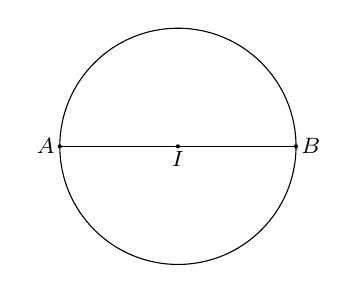
\begin{tikzpicture}[scale=.75,font=\footnotesize,line join=round,line cap=round,>=stealth]
				\draw  (0,0) circle (2cm);
				\fill (-2,0) circle  (1pt) node[left]{$A$};
				\fill (2,0) circle  (1pt) node[right]{$B$};
				\fill (0,0) circle (1pt) node[below]{$I$}; 
				\draw (-2,0)--(2,0); 
			\end{tikzpicture}
		} 
	} 
\end{bt}

% từ: cau-hoi/lop10/0H9_Phuong_phap_toa_do_trong_mat_phang/0H9-3-2_Phuong_trinh_duong_thang.tex
\begin{bt}%[0H9H3-2]%[Tex_Toan10, Lương Như Quỳnh]%[ma:8c7520d4]
	Trong mặt phẳng tọa độ, cho tam giác $ ABC $ với $ A(6;-2) $, $ B(4;2) $, $ C(5;-5) $. Viết phương trình đường tròn ngoại tiếp tam giác đó.
	\loigiai{
		Các đoạn thẳng $ AB $, $ AC $ tương ứng có trung điểm là $ M(5;0) $, $ N\left(\dfrac{11}{2};-\dfrac{7}{2}\right) $.\\
		Đường thẳng trung trực $ \Delta_1$ của đoạn thẳng $ AB $ đi qua $ M(5;0) $ và có một véc-tơ pháp tuyến $ \overrightarrow{AB}(-2;4) $.\\
		Vì $ \overrightarrow{AB}(-2;4) $ cùng phương với $ \overrightarrow{n}_1(1;-2) $ nên $ \Delta_1$ cũng nhận $ \overrightarrow{n}_1(1;-2) $ là một véc-tơ pháp tuyến.\\
		Do đó phương trình của $ \Delta_1$ là \[1(x-5)-2(y-0)=0\text{ hay } x-2y-5=0.\]
		Đường thẳng trung trực $ \Delta_2$ của đoạn thẳng $ AC $ đi qua $ N\left(\dfrac{11}{2};-\dfrac{7}{2}\right) $ và có véc-tơ pháp tuyến $ \overrightarrow{AC}(-1;-3) $.\\
		Do đó phương trình của $ \Delta_2$ là \[-1\left(x-\dfrac{11}{2}\right)-3\left(y+\dfrac{7}{2}\right)=0\text{ hay } x+3y+5=0.\]
		Tâm $ I $ của đường tròn $ (C) $ cách đều ba điểm $ A $, $ B $, $ C $ nên $ I $ là giao điểm của $ \Delta_1$ và $ \Delta_2$.\\
		Vậy tọa độ của $ I $ là nghiệm của hệ phương trình $ \heva{&x-2y-5=0\\&x+3y+5=0.} $\\
		Suy ra $ I(1;-2) $. Đường tròn $ (C) $ có bán kính là $ IA=5 $. Vậy phương trình của $ (C) $ là 
		\[(x+2)^2+(y+1)^2=25.\]
	}
\end{bt}

% từ: cau-hoi/lop10/0H9_Phuong_phap_toa_do_trong_mat_phang/0H9-3-8_Bai_toan_thuc_te_PP_toa_do_hoa.tex
\begin{bt}%[0H9V3-8]%[ma:627e629a]
	Để tham gia một phòng tập thể dục, người tập phải trả một khoản phí tham gia ban đầu và phí sử dụng phòng tập. Đường thẳng $\Delta$ ở hình bên dưới biểu thị tổng chi phí (đơn vị: triệu đồng) tham gia một phòng tập thể dục theo thời gian tập của một người (đơn vị: tháng).\\
	\begin{enumerate}
		\item Viết phương trình của đường thẳng $\Delta$.
		\item Cho biết giao điểm của đường thẳng $\Delta$ với trục tung trong tình huống này có ý nghĩa gì.
		\item Tính tổng chi phí mà người đó phải trả khi tham gia phòng tập thể dục với thời gian $12$ tháng.
	\end{enumerate}
	\begin{center}
		\begin{tikzpicture}[scale=0.8, font=\footnotesize, line join=round, line cap=round, >=stealth]
			\draw[->,line width = 1pt] (-1,0)--(0,0) node[below left]{$O$}--(8,0) node[below]{$x$};
			\draw[->,line width =1 pt] (0,-1)--(0,8) node[right]{$y$};
			\draw [thick,domain=0:6,samples=100] 
			plot (\x,{(\x)+3/2}) node [above left] {$\Delta$};
			\draw (0,1) node [left] {$1$} circle (1pt);
			\draw (0,1.5) node [left] {$1,5$} circle (1pt);		
			\draw (0,5) node [left] {$5$} circle (1pt);
			\draw (0.5,0) node [below] {$1$} circle (1pt);
			\draw (3.5,0) node [below] {$7$} circle (1pt);
			\draw (6,0) node [below] {$12$} circle (1pt);
			\draw [dashed] (3.5,0)--(3.5,5)--(0,5);
		\end{tikzpicture}	
	\end{center}
	\loigiai{
		\begin{enumerate}
			\item Đường thẳng $\Delta$ đi qua hai điểm lần lượt có tọa độ $(0;\,1{,}5)$ và $(7;\,5)$ nên $\Delta$ có phương trình là
			$$\dfrac{x-0}{7-0}=\dfrac{y-1{,}5}{5-1{,}5}\Leftrightarrow\dfrac{x}{7}=\dfrac{y-1{,}5}{3{,}5}\Leftrightarrow\dfrac{x}{2}=\dfrac{y-1{,}5}{1}\Leftrightarrow y=\dfrac{x}{2}+1{,}5.$$
			\item Giao điểm của đường thẳng $\Delta$ với trục $Oy$ ứng với $x=0$. Thời điểm $x=0$ cho biết mức phí tham gia ban đầu và phí sử dụng phòng tập. Khi $x=0$ thì $y=1{,}5$, vì vậy chi phí tham gia ban đầu và phí sử dụng phòng tập là $1500000$ đồng.
			\item $12$ tháng đầu tiên ứng với $x=12$. Do đó $y=\dfrac{12}{2}+1{,}5=7{,}5$.\\
			Vậy tổng chi phí mà người đó phải trả khi tham gia phòng tập thể dục với thời gian $12$ tháng đầu tiên là $7500000$ đồng.
		\end{enumerate}
		
	}
\end{bt}

% từ: cau-hoi/lop10/0H9_Phuong_phap_toa_do_trong_mat_phang/0H9-5-0_Bai_toan_tong_hop_thuc_te_PP_toa_do_hoa_3_duo.tex
\begin{bt}%[0H9H5-0]%[10EX- Tex hóa CD -CT-hk2-Thầy Trịnh Xuân]%[ma:507f65e1]
	\immini{
		Một tháp triển lãm có mặt cắt hình hypebol có phương trình $\dfrac{x^2}{18^2}-\dfrac{y^2}{36^2}=1$. Cho biết chiều cao của tháp là $100\,\mathrm{m}$ và khoảng cách từ nóc tháp đến tâm đối xứng của hypebol bằng khoảng cách từ tâm đối xứng đến đáy. Tính bán kính nóc và bán kính đáy của tháp.
	}{
		\begin{tikzpicture}[line join = round, line cap = round,>=stealth,scale=1]
			\draw[->] (-2,0) -- (2,0) node[right] {$x$};
			\draw[->] (0,-3) -- (0,3.2) node[above] {$y$};
			\draw[domain=-2:2,smooth, samples=150] plot ({(0.35*(\x))^(2)+0.5},\x);
			\draw[domain=-2:2,smooth, samples=150] plot (-{(0.35*(\x))^(2)-0.5},\x);
			\draw (0,2.05) ellipse (1 and 0.4);
			\draw[dashed] (0,-2.05) ellipse (1 and 0.4);
			\draw (0,-2.05)+(0:1 and 0.4) arc (0:-180:1 and 0.4);
			\fill (0,0)node[above right]{$O$} circle (1pt);
		\end{tikzpicture}
	}
	\loigiai{
		Do tính đối xứng của hypebol nên ta có hai bán kính của nóc và đáy tháp đều bằng $r$.\\
		Do điểm $M(r;50)$ nằm trên hypebol nên thay tọa độ của điểm $M$ vào phương trình của hypebol ta có:\\ $\dfrac{r^2}{18^2}-\dfrac{50^2}{36^2}=1 \Rightarrow r=18\sqrt{1+\dfrac{50^2}{36^2}} \approx 31(\mathrm{m})$.\\
		Vậy bán kính của nóc và đáy của tháp bằng $31\,\mathrm{m}$.
	}
\end{bt}

% từ: cau-hoi/lop10/0H9_Phuong_phap_toa_do_trong_mat_phang/0H9-5-0_Bai_toan_tong_hop_thuc_te_PP_toa_do_hoa_3_duo.tex
\begin{bt}%[0H9H5-0]%[ma:2eb547a4]
    \immini[thm]{
    Trước một tòa nhà, người ta làm một cái hồ bơi có dạng hình elip với độ dài hai bán trục lần lượt là $3$ m và $5$ m. Xét hệ trục tọa độ $Oxy$ (đơn vị trên các trục là mét) có hai trục tọa độ chứa hai trục của elip, gốc tọa độ $O$ là tâm của elip (hình). Xét các điểm $M$, $N$ cùng thuộc trục lớn của elip và đều cách $O$ một khoảng bằng $4$ m về hai phía của $O$. Tính tổng khoảng cách từ một điểm bất kì trên đường elip đến $M$ và $N$.    
    }{
    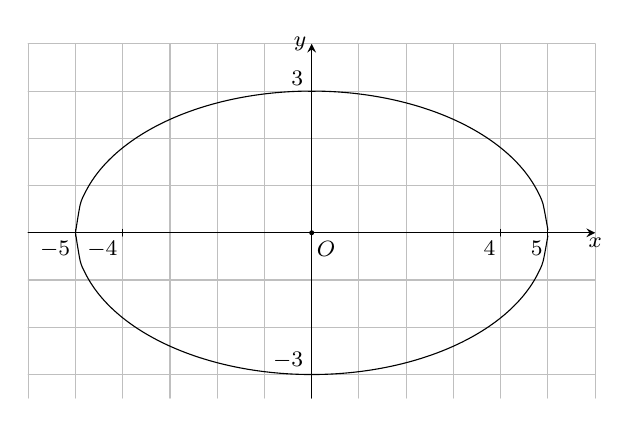
\begin{tikzpicture}[scale=0.6,line cap=round,line join=round,>=stealth,x=1.0cm,y=1.0cm]
        \draw[step=1cm,color=black!25!] (-6,-3.5) grid (6,4);
        \draw[->,color=black] (-6,0.) -- (6,0.) node[below] {\footnotesize $x$};
        \foreach \x in {-5,-4,4,5}
        \draw[shift={(\x,0)},color=black] (0pt,2pt) -- (0pt,-2pt) node[below left] {\footnotesize $\x$}; 
        \draw[->,color=black] (0.,-3.5) -- (0.,4) node[left] {\footnotesize $y$};
        \foreach \y in {-3,3} 
        \draw[shift={(0,\y)},color=black] (2pt,0pt) -- (-2pt,0pt) node[above left] {\footnotesize $\y$}; 
        \draw[color=black] (0pt,-10pt) node[right] {\footnotesize $O$};
        \clip(-6,-3.5) rectangle (6,4);
        \draw[smooth,samples=100,domain=-5:5] plot(\x,{3/5*sqrt(25-(\x)^2)});
        \draw[smooth,samples=100,domain=-5:5] plot(\x,{-3/5*sqrt(25-(\x)^2)});
        \fill (0cm,0cm) circle (1.5pt);  
    \end{tikzpicture}
    }
    \shortans[]{$10$}
    \loigiai{
    Phương trình chính tắc của đường elip là $\dfrac{x^2}{5^2}+ \dfrac{y^2}{3^2}=1 \Leftrightarrow \dfrac{x^2}{25}+ \dfrac{y^2}{9}=1$.\\
    Ta có $a=5$, $b=3 \Rightarrow c^2= a^2-b^2=16 \Rightarrow c=4$.\\ 
    Các tiêu điểm của elip  là $\left(-4;0\right)$ và $\left(4;0\right)$.\\ 
    Do đó, hai điểm $M,N$ là hai tiêu điểm của elip.\\ 
    Vì vậy, tổng khoảng cách từ một điểm trên elip đến hai điểm $M,N$ bằng $2a=10$ m. 
    }
\end{bt}

% từ: cau-hoi/lop10/0H9_Phuong_phap_toa_do_trong_mat_phang/0H9-5-0_Bai_toan_tong_hop_thuc_te_PP_toa_do_hoa_3_duo.tex
\begin{bt}%[0H9V5-0]%[Câu 22]%[ma:0df60d0e]
\immini{
	Mặt Trăng chuyển động quanh Trái Đất theo quỹ đạo là một elip mà tâm Trái Đất là một tiêu điểm. Elip đó có $A_1 A_2=768\,800 \mathrm{~km}$ và $B_1 B_2=767\,640 \mathrm{~km}$. Khoảng cách ngắn nhất từ tâm Trái Đất đến Mặt Trăng là $ a $ ($ a $ được làm tròn đến hàng đơn vị). Tìm phần nguyên của số $ \dfrac{a}{1\,000}  $.  ($ 1 $ đơn vị đo trên trục tọa độ tương ứng với $ 1 $ km trên thực tế).
}
{
	\begin{tikzpicture}[scale=1, font=\footnotesize, line join=round, line cap=round, >=stealth]
		\path 
		(0,0) coordinate (O)
		(2.5,0) coordinate (A_2)
		(-2.5,0) coordinate (A_1)
		(0,-1.5) coordinate (B_1)
		(0,1.5) coordinate (B_2)
		({-sqrt(2.5^2-1.5^2)},0) coordinate (F)
		($(O)+(45:2.5 cm and 1.5 cm)$) coordinate (M)
		;
		\draw [->] (-3.2,0)--(3.5,0) node[above]{$x$} ;
		\draw [->] (0,-2.3)--(0,2.3) node[left]{$y$} ;
		\draw (O) ellipse (2.5 cm and 1.5 cm) ;
		\draw[fill=black] (-1.2,0) circle(1.5pt) node[below]{\text{Trái Đất}} ;
		\draw [fill=black] (M) circle(1.5pt) node[above right]{\text{Mặt Trăng}} ;
		\draw [fill=black] (0,0) circle(1pt) node[above left]{$O$} ;
		\foreach \x/\g in{A_1/-130,A_2/-50,B_1/-130,B_2/140}
		\fill[black](\x)circle(1.1pt) ($(\x)+(\g:3.5mm)$) node{$\x$}; 
	\end{tikzpicture}
}
\shortans{$ 363 $}
\loigiai{
	Phương trình chính tắc của elip có dạng $\dfrac{x^2}{a^2} + \dfrac{y^2}{b^2} = 1$. \\
	Theo giả thiết $A_1 A_2=768\,800 \mathrm{~km}$,  $B_1 B_2=767\,640 \mathrm{~km}$ suy ra $a= 384\,400$ và $b=383\,820$.  \\
	Vậy phương trình của elip là 
	\[
	\dfrac{x^2}{384\,400^2}+\dfrac{y^2}{383\,820^2} =1.
	\]
	Gọi $M$, $F_1$ là vị trí của Mặt Trăng và Trái Đất trên hệ trục tọa độ. \\
	$M$ là điểm thuộc elip $\dfrac{x^2}{a^2}+\dfrac{y^2}{b^2}=1$ nên $-a \leq x_M\leq a$. \\
	Suy ra $MF_1=a+\dfrac{c}{a}\cdot x_M \geq a-\dfrac{c}{a}\cdot a=a-c$. \\
	Vậy khoảng cách ngắn nhất từ Trái Đất đến Mặt Trăng là 
	\[a-c=a-\sqrt{a^2-b^2}=384\,400-\sqrt{384\,400^2-383\,820^2}\approx 363\,292\mathrm{~km}.\]
}
\end{bt}

% từ: cau-hoi/lop10/0H9_Phuong_phap_toa_do_trong_mat_phang/0H9-5-0_Bai_toan_tong_hop_thuc_te_PP_toa_do_hoa_3_duo.tex
\begin{bt}%[0H9V5-0]%[ma:f2181d9f]
	\immini[thm]{
		Một gương lõm có mặt cắt hình parabol (hình bên), có tiêu điểm cách đỉnh $5$ cm. Cho biết bề sâu của gương là $45$ cm, Tính khoảng cách $AB$.
	}{
		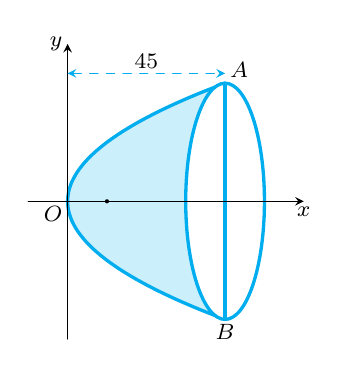
\begin{tikzpicture}[scale=0.5, font=\footnotesize, line join=round, line cap=round, >=stealth,
			declare function={ f(\y)=4/9*(\y)^2;}
			]
			\draw[smooth, color=cyan, fill=cyan!20, line width=1.2pt, domain=-3:3,variable=\y] plot({f(\y)},{\y});
			\draw[color=cyan, fill=white, line width=1.2pt, rotate=90] (0,-4) ellipse (3cm and 1cm);
			\draw[color=cyan, line width=1.2pt] (4,3)--(4,-3);
			\draw[->] (-1,0)--(6,0) node [below]{$x$};
			\draw[->] (0,-3.5)--(0,4) node [left]{$y$};
			\node at (0,0) [below left]{$O$};
			\node at (4,3) [above right]{$A$};
			\node at (4,-3) [below]{$B$};
			\fill (1,0) circle (1.5pt);
			\draw[<->, dashed, color=cyan] (0,3.25)--(4,3.25);
			\node at (2,3.25) [above]{$45$};
		\end{tikzpicture}
	}
\shortans{$60$}
	\loigiai{
		Do tiêu điểm cách đỉnh $5$ cm nên $\dfrac{p}{2}=5 \Leftrightarrow p=10$.\\
		Nên phương trình parabol $(P)$ là $y^2=20x$.\\
		Mà bề sâu của gương là $45$ cm nên ta có $x_A=x_B=45$.\\
		Suy ra $y_A=30$, $y_B=-30$.\\
		Vậy $AB=y_A-y_B=60$ cm.
	}
\end{bt}

% từ: cau-hoi/lop11/1C2_Ly_thuyet_do_thi/1C2-3-1_Bai_toan_tim_duong_di_ngan_nhat.tex
\begin{bt}%[1C2B3-1]%[ma:a9eefc78]
	Cho cấp số nhân $\left(u_n\right)$. Tìm số hạng đầu $u_1$, công bội  $q$ trong mỗi trường hợp sau:
	\begin{multicols}{2}
		\begin{enumerate}[a)]
			\item $u_6=192$ và  $u_7=384$;
			\item  $u_1+u_2+u_3=7$ và $u_5-u_2=14$.
		\end{enumerate}
	\end{multicols}
	\loigiai{ 
		\begin{enumerate}[a)]
			\item  $u_6=192$ và $u_7=384$;\\
			Ta có $\heva{u_6=192  \\ u_7=384} \Leftrightarrow \heva{u_1.q^5=192 \\ u_1.q^6=384} \Leftrightarrow \heva{u_1=6\\ q=2}$.\\
			Vậy số hạng  đầu $u_1=6$, công bội $q=2$.
			 \item $u_1+u_2+u_3=7$ và $u_5-u_2=14$.\\
			Ta có \begin{eqnarray*}
			&&\heva{u_1+u_2+u_3&=7  \\ u_5-u_2&=14} \Leftrightarrow \heva{u_1.(1+q+q^2)&=7 \\ u_1.q.(q^3-1)&=14} \Leftrightarrow \heva{u_1.(1+q+q^2)=7\\ q(q-1)=2} \\
			&\Leftrightarrow&  \heva{u_1.(1+q+q^2)=7\\ q^2-q-2=0.}\Leftrightarrow \hoac{\heva{u_1=1 \\ q=2}\\\heva{u_1&=7 \\ q&=-1.}}
		\end{eqnarray*}
		Vậy có  hai cấp số nhân thỏa mãn đề bài số hạng đầu $u_1=1$, công sai $q=2$; số hạng đầu $u_1=7$, công sai $q=-1$.
	\end{enumerate}
 }
\end{bt}

% từ: cau-hoi/lop11/1D1_Ham_so_luong_giac_va_phuong_trinh_luong/1D1-2-1_Cau_hoi_ly_thuyet.tex
\begin{ex}%[1D1Y2-1]%[ma:89c77e36]
	Khẳng định nào  sau đây là đúng
	\choice 
		{$\cos x =0 \Leftrightarrow x =\dfrac{\pi}{2} +k2\pi; k \in  \mathbb{Z}$}
		{\True $\cos x =-1  \Leftrightarrow x =\pi +k2 \pi; k \in \mathbb{Z}$}
		{$\sin x =0 \Leftrightarrow x = k2\pi;  k \in \mathbb{Z}$}
		 {$\tan x =0 \Leftrightarrow x = k 2\pi; k \in \mathbb{Z}$}
	\loigiai{ 
		Ta có $\cos x =-1 \Leftrightarrow  x =\pi +k2 \pi; k \in \mathbb{Z}$.
	 }
\end{ex}

% từ: cau-hoi/lop11/1D1_Ham_so_luong_giac_va_phuong_trinh_luong/1D1-2-3_Bien_doi_rut_gon_bieu_thuc_luong_giac_chung_m.tex
\begin{ex}%[1D1H2-3]%[ma:4911c3a7]
	Cho hai góc nhọn $a$ và $b$. Biết $\cos a=\dfrac{1}{3}$ và $\cos b=\dfrac{1}{4}$. Tính giá trị của 
	$P=(\cos a\cdot\cos b)^2-(\sin a\cdot\sin  b)^2 .$ (làm tròn đến chục)
	\shortans{-0,8} 
	 \loigiai{
		 Ta có\\
		$\begin{aligned}
		 {P}&=(\cos a\cos b)^2-(\sin a\sin b)^2=(\cos a\cos b)^2-\left(1-\cos ^2 a\right)\left(1-\cos ^2 b\right)\\
		 &=\left(\dfrac{1}{12}\right)^2-\dfrac{8}{9}\cdot\dfrac{15}{16}=-\dfrac{119}{144}\approx-0{,}8.
\end{aligned}$}
\end{ex}

% từ: cau-hoi/lop11/1D1_Ham_so_luong_giac_va_phuong_trinh_luong/1D1-2-3_Bien_doi_rut_gon_bieu_thuc_luong_giac_chung_m.tex
\begin{ex}%[1D1H2-3]%[ma:9ff1344f]
	Rút gọn biểu thức  $A=2\cos ^4x-\sin ^4x+\sin ^2x\cos ^2x+3\sin ^2x$.
	 \shortans{2}
	 \loigiai{
		\begin{align*}
			A&=2\cos ^4x-\sin ^4x+\sin  ^2x\cos ^2x+3\sin ^2x\\
			&=\cos ^4x-\sin ^4x+\cos ^4x+\sin  ^2x\cos ^2x+3\sin ^2x\\
			&=\cos ^2x-\sin  ^2x+\cos ^2x+3\sin ^2x\\
			 &=2\cos ^2x+2\sin ^2x=2.
		\end{align*}
	} 
\end{ex}

% từ: cau-hoi/lop11/1D1_Ham_so_luong_giac_va_phuong_trinh_luong/1D1-2-3_Bien_doi_rut_gon_bieu_thuc_luong_giac_chung_m.tex
\begin{bt}%[1D1V2-3]%[ma:c9d2b36b]
% nguon: Archive/2024/SP-K10-K11-LyVanHoang_TVN-023/11. C1-LuongGiac-lvhoang_TVN-023/dataC1K11/Bai-1-Dang-8-RutGonBieuThucLuongGiac.tex #1824

	Cho $\sin a+\cos a=m$. Tính giá trị của $\sin a\cos a$, từ đó tính giá trị của $\left|\sin a-\cos a\right|$ theo $m$.
	\loigiai{
		\begin{itemize}
			\item Ta có $\sin a+\cos a =m$. \\
			Suy ra $(\sin a+\cos a)^2=m^2\Leftrightarrow 1+2\sin a\cos a=m^2\Leftrightarrow \sin a\cos a=\dfrac{m^2-1}{2}$.
			\item Ta có 
			$$(\sin a-\cos a)^2=1-2\sin a\cos a=1-(m^2-1)=2-m^2.$$
			Vậy $|\sin a-\cos a|=\sqrt{2-m^2}$.
		\end{itemize}
	}
\end{bt}

% từ: cau-hoi/lop11/1D1_Ham_so_luong_giac_va_phuong_trinh_luong/1D1-2-4_Cac_goc_luong_giac_co_lien_quan_dac_biet_bu_n.tex
\begin{ex}%[1D1N2-4]%[ma:ce5ab1a2]
	Rút gọn biểu thức $S=\cos \left(\dfrac{\pi}{2}-x\right)\sin \left(\pi-x\right)-\sin \left(\dfrac{\pi}{2}-x\right)\cos \left(\pi-x\right)$ ta  được
	\choice 
		 {$S=0$}
		{$S=\sin  ^2x-\cos ^2x$}
		{$S=2\sin  x\cos x$}
		{\True  $S=1$}
	 \loigiai{
		 Ta có
		\begin{align*}
			S&=\cos \left(\dfrac{\pi}{2}-x\right)\cdot \sin  \left(\pi-x\right)-\sin \left(\dfrac{\pi}{2}-x\right)\cdot \cos \left(\pi-x\right)\\
			 &=\sin x\cdot \sin x-\cos x\cdot \left(-\cos x\right)=\sin ^2x+\cos ^2x=1.
		\end{align*}
	 }
\end{ex}

% từ: cau-hoi/lop11/1D1_Ham_so_luong_giac_va_phuong_trinh_luong/1D1-3-2_Ap_dung_cong_thuc_cong.tex
\begin{bt}%[1D1V3-2]%[ma:d45a8821]
% nguon: Archive/2024/TOAN_11_XE/TOAN_11_XE/data4/11C1/KNTT-1.2.tex #1154
%[MANDALA] 
	Cho tam giác $A B C$ có $\widehat{B}=75^{\circ}; \widehat{C}=45^{\circ}$ và $a=B C=12 \mathrm{~cm}$.
	\begin{enumerate}
		\item Sử dụng công thức $S=\dfrac{1}{2} a b \sin C$ và định lí sin, hãy chứng minh diện tích của tam giác $A B C$ cho bởi công thức
		$$
		S=\dfrac{a^2 \sin B \sin C}{2 \sin A} .
		$$
		\item Sử dụng kết quả ở câu $1$ và công thức biến đổi tích thành tổng, hãy tính diện tích $S$ của tam giác $A B C$.
	\end{enumerate}
	\loigiai{
		\begin{enumerate}
			\item Ta có $\dfrac{a}{\sin A}=\dfrac{b}{\sin B}$ nên $b=\dfrac{a\sin B}{\sin A}$.\\
			Khi đó $S=\dfrac{1}{2} a b \sin C=\dfrac{1}{2}a\cdot\dfrac{a\sin B}{\sin A}\sin C=\dfrac{a^2 \sin B \sin C}{2 \sin A} $.
			\item Ta có $\sin B\sin C=\dfrac{1}{2}\left[\cos\left(B-C\right)-\cos\left(B+C\right)\right]=\dfrac{1}{2}\left(\cos30^\circ-\cos120^\circ\right)=\dfrac{1+\sqrt{3}}{4}$.
			\\
			Lại có $\sin A=\sin\left(180^\circ-B-C\right)=\sin60^\circ=\dfrac{\sqrt{3}}{2}$.\\
			Diện tích $S$ của tam giác $A B C$ là $S=\dfrac{a^2 \sin B \sin C}{2 \sin A}=\dfrac{12^2\cdot\dfrac{1+\sqrt{3}}{4}}{2\cdot\dfrac{\sqrt{3}}{2}}=36+12\sqrt{3}\,\mathrm{cm}^2$.
		\end{enumerate}
	}
\end{bt}

% từ: cau-hoi/lop11/1D1_Ham_so_luong_giac_va_phuong_trinh_luong/1D1-3-3_Ap_dung_cong_thuc_nhan_doi_ha_bac.tex
\begin{ex}%[1D1N3-3]%[ma:83a8c4fc]
	Với $\alpha$ là số thực bất kỳ, trong các mệnh đề sau,  mệnh đề nào \textbf{sai}?
	\choice 
		{$\sin 2\alpha =2\sin \alpha \cdot \cos  \alpha$}
		 {$\cos 2\alpha =2\cos^2\alpha-1$}
		 {$\cos 2\alpha =-2\sin^2\alpha+1$}
		{\True $\cos 2\alpha=\sin^2\alpha-\cos^2\alpha$} 
	 \loigiai{
		Ta có $\sin 2\alpha=2\sin \alpha  \cdot \cos \alpha $; $\cos 2\alpha =\cos^2\alpha -\sin^2\alpha =2\cos^2\alpha-1=1-2\sin^2\alpha$.
	 }
\end{ex}

% từ: cau-hoi/lop11/1D1_Ham_so_luong_giac_va_phuong_trinh_luong/1D1-3-3_Ap_dung_cong_thuc_nhan_doi_ha_bac.tex
\begin{ex}%[1D1N3-3]%[ma:bba23c1f]
	Cho biết $\sin \alpha = \dfrac{1}{3}$  và $\dfrac{\pi}{2} < \alpha < \pi$.
	\choiceTF 
		{\True $\cos \alpha  = -\dfrac{2\sqrt{2}}{3}$}
		{\True $\sin 2\alpha  = -\dfrac{4\sqrt{2}}{9}$}
		 {\True $\cos 2\alpha = \dfrac{7}{9}$}
		{$\cot 2\alpha = \dfrac{7\sqrt{2}}{8}$} 
	\loigiai{ 
		\begin{itemchoice}
			\itemch Ta có $\dfrac{\pi}{2}  < \alpha < \pi$ nên $\cos\alpha < 0$.\\
			Ta có $\cos^2 \alpha = 1 - \sin^2 \alpha =  1 - \dfrac{1}{9} = \dfrac{8}{9} \Rightarrow \cos\alpha = -\dfrac{2\sqrt{2}}{3}$.
			\itemch  Ta có $\sin 2\alpha = 2\sin\alpha\cos\alpha = 2 \cdot \dfrac{1}{3} \cdot \left(-\dfrac{2\sqrt{2}}{3}\right) = -\dfrac{4\sqrt{2}}{9}$.
			\itemch Ta có $\cos 2\alpha = 1 - 2\sin^2 \alpha = 1 - 2\left(\dfrac{1}{3}\right)^2 = 1 - 2 \cdot  \dfrac{1}{9} = \dfrac{7}{9}$.
			\itemch Ta có $\tan 2\alpha = \dfrac{\sin 2\alpha}{\cos 2\alpha} =  \frac{-\dfrac{4\sqrt{2}}{9}}{\dfrac{7}{9}} = -\dfrac{4\sqrt{2}}{7} \Rightarrow \cot 2\alpha = \dfrac{1}{\tan 2\alpha} = -\dfrac{7}{4\sqrt{2}} = -\dfrac{7\sqrt{2}}{8}$.
		\end{itemchoice}
	} 
\end{ex}

% từ: cau-hoi/lop11/1D1_Ham_so_luong_giac_va_phuong_trinh_luong/1D1-3-4_Ap_dung_cong_thuc_bien_doi_tich_tong.tex
\begin{bt}%[1D1V3-4]%[ma:6f5832e4]
% nguon: Archive/2024/SP-K10-K11-LyVanHoang_TVN-023/11. C1-LuongGiac-lvhoang_TVN-023/dataC1K11/Bai2-Dang3-Congthucbiendoitichthanhtong.tex #1783
%[Huỳnh Đức Vũ, dự án bài giảng K10-11]
	Biến đổi thành tổng các biểu thức sau
	\begin{listEX}[2]
		\item $G= 2\sin x\sin 2x\sin 3x$.
		\item $H= 8\cos x\sin 2x\sin 3x$.
		\end{listEX}
	\loigiai{
		\begin{enumerate}
			\item $G= 2\sin x\sin 2x\sin 3x= \left( \cos x- \cos 3x\right)\sin 3x= \dfrac{1}{2}\left( \sin 2x+ \sin 4x- \sin 6x\right)$.
			\item 
			\begin{eqnarray*}
			H &=& 8\cos x\sin 2x\sin 3x=(2\sin2x\cos x)\cdot4\sin3x=(\sin x+\sin 3x)\cdot4\sin3x \\
			&=&2(2\sin3x\sin x+2\sin^23x)=2(\cos 2x-\cos 4x+1-\cos6x).
			\end{eqnarray*}
		\end{enumerate}
	}
\end{bt}

% từ: cau-hoi/lop11/1D1_Ham_so_luong_giac_va_phuong_trinh_luong/1D1-3-4_Ap_dung_cong_thuc_bien_doi_tich_tong.tex
\begin{bt}%[1D1N3-4]%[ma:144a0af2]
% nguon: Archive/2024/SP-K10-K11-LyVanHoang_TVN-023/11. C1-LuongGiac-lvhoang_TVN-023/dataC1K11/Bai2-Dang4-Congthucbiendoitongthanhtich.tex #2071
%[BG - 11 New - 4in1, Lê Đạt]
	Tính
	\begin{listEX}[2]
		\item $\sin \dfrac{11 \pi}{12}-\sin \dfrac{5 \pi}{12}$.
		\item $\cos 105^{\circ}+\cos 15^{\circ}$.	
	\end{listEX}	
	\loigiai{
		\begin{listEX}[1]
			\item $\sin \dfrac{11 \pi}{12}-\sin \dfrac{5 \pi}{12}=2 \cos \dfrac{\dfrac{11 \pi}{12}+\dfrac{5 \pi}{12}}{2} \sin \dfrac{\dfrac{11 \pi}{12}-\dfrac{5 \pi}{12}}{2}=2 \cos \dfrac{2 \pi}{3} \sin \dfrac{\pi}{4}=2 \cdot\left(-\dfrac{1}{2}\right) \cdot \dfrac{\sqrt{2}}{2}=-\dfrac{\sqrt{2}}{2}$. 
			\item $\cos 105^{\circ}+\cos 15^{\circ}=2 \cos \dfrac{105^{\circ}+15^{\circ}}{2} \cos \dfrac{105^{\circ}-15^{\circ}}{2}=2 \cos 60^{\circ} \cos 45^{\circ}=2 \cdot \dfrac{1}{2} \cdot \dfrac{\sqrt{2}}{2}=\dfrac{\sqrt{2}}{2}$.
		\end{listEX}	
	}
\end{bt}

% từ: cau-hoi/lop11/1D1_Ham_so_luong_giac_va_phuong_trinh_luong/1D1-3-4_Ap_dung_cong_thuc_bien_doi_tich_tong.tex
\begin{bt}%[1D1H3-4]%[ma:9aa6f04e]
% nguon: Archive/2024/TOAN_11_XE/TOAN_11_XE/data4/11C1/KNTT-1.2.tex #1144
%%[DCHT Toán 11 - KNTT -Nguyễn Thành Nhân]
	Biến đổi các tổng sau thành tích
	\begin{listEX}[2]
		\item $A=\sin 5x+\sin 6x+\sin 7x+\sin 8x$.
		\item $B=\sin x-\sin 3x+\sin 7x-\sin 5x$.
		\item $C=\cos 7x+\sin 3x+\sin 2x-\cos 3x$.
		\item $D=\sin 35^\circ +\cos 40^\circ +\sin 55^\circ +\cos 20^\circ$.
	\end{listEX}
	\loigiai{
		\begin{enumerate}
			\item \allowdisplaybreaks\begin{eqnarray*}
				A&=&\left(\sin 8x+\sin 5x\right)+\left(\sin 7x+\sin 6x\right)\\
				&=&2\sin \dfrac{13x}{2}\cos \dfrac{3x}{2}+2\sin \dfrac{13x}{2}\cos \dfrac{x}{2}\\
				&=&2\sin \dfrac{13x}{2}\left(\cos \dfrac{3x}{2}+\cos \dfrac{x}{2}\right).
			\end{eqnarray*}
			\item \allowdisplaybreaks\begin{eqnarray*}
				B&=&\left(\sin 7x+\sin x\right)-\left(\sin 5x+\sin 3x\right)\\
				&=&2\sin 4x\cos 3x-2\sin 4x\cos x\\
				&=&2\sin 4x\left(\cos 3x-\cos x\right).
			\end{eqnarray*}
			\item \allowdisplaybreaks\begin{eqnarray*}
				C&=&\left(\cos 7x-\cos 3x\right)+\left(\sin 3x+\sin 2x\right)\\
				&=&-2\sin 5x\sin 2x+2\sin \dfrac{5x}{2}\cos \dfrac{x}{2}\\
				&=&2\sin \dfrac{5x}{2}\left(-2\cos \dfrac{5x}{2}\sin 2x+\cos \dfrac{x}{2}\right).
			\end{eqnarray*}
			\item \allowdisplaybreaks\begin{eqnarray*}
				D&=&\left(\sin 55^\circ +\sin 35^\circ\right)+\left(\cos 40^\circ +\cos 20^\circ\right)\\
				&=&2\sin 45^\circ\cos 10^\circ +2\cos 30^\circ\cos 10^\circ \\
				&=&2\cos 10^\circ\left(\sin 45^\circ +\cos 30^\circ\right).
			\end{eqnarray*}
		\end{enumerate}
	}
\end{bt}

% từ: cau-hoi/lop11/1D1_Ham_so_luong_giac_va_phuong_trinh_luong/1D1-3-5_Ket_hop_nhieu_cong_thuc_luong_giac.tex
\begin{ex}%[1D1H3-5]%[ma:6319dd8a]
	Cho biết $\sin\alpha=\dfrac{1}{3}$ và $\dfrac{\pi}{2}<\alpha <\pi $. Khi  đó
	 \choiceTF
		 {\True $\cos\alpha=-\dfrac{2\sqrt 2}{3}$}
		{\True $\sin  2\alpha=-\dfrac{4\sqrt 2}{9}$}
		{\True  $\cos 2\alpha=\dfrac{7}{9}$}
		{$\cot 2\alpha=\dfrac{7\sqrt 2}{8}$} 
	\loigiai{ 
		Vì $\dfrac{\pi}{2}<\alpha<\pi$ nên $\cos \alpha<0$. Ta có\\ 
		\begin{itemize}
			\item  $\cos^2\alpha=1-\sin^2\alpha=1-\dfrac{1}{9}=\dfrac{8}{9}\Rightarrow\cos\alpha=-\dfrac{2\sqrt 2}{3}$.
			\item $\sin2\alpha=2\sin\alpha\cos\alpha=2\cdot\dfrac{1}{3}\cdot\left(-\dfrac{2\sqrt  2}{3}\right)=-\dfrac{4\sqrt 2}{9}$.
			\item $\cos 2\alpha=1-2\sin ^2\alpha=1-2\left(\dfrac{1}{3}\right)^2=\dfrac{7}{9}$. 
			\item $\tan 2\alpha=\dfrac{\sin 2\alpha}{\cos 2\alpha}=-\dfrac{4\sqrt 2}{7}; \cot 2\alpha=\dfrac{1}{\tan 2\alpha}=-\dfrac{7\sqrt  2}{8}$.
		\end{itemize}
	} 
\end{ex}

% từ: cau-hoi/lop11/1D1_Ham_so_luong_giac_va_phuong_trinh_luong/1D1-3-5_Ket_hop_nhieu_cong_thuc_luong_giac.tex
\begin{ex}%[1D1V3-5]%[ma:220a26f0]
	 Cho góc $\alpha $ thỏa mãn $\sin 2\alpha=-\dfrac{4}{5}$ và $\dfrac{3\pi}{4}<\alpha <\pi $. Tính $ P=\sin\alpha-\cos\alpha$ (làm tròn đến hàng phần trăm).
	 \shortans{1,34}
	\loigiai{ 
	Vì $\dfrac{3\pi}{4}<\alpha <\pi $ suy ra $\left\{\begin{array}{l}
	\sin\alpha  > 0\\
	\cos\alpha <  0
\end{array}\right.$ nên $\sin\alpha-\cos\alpha > 0$.\\
Ta có  $\left(\sin\alpha-\cos\alpha\right)^2=1-\sin 2\alpha=1+\dfrac{4}{5}=\dfrac{9}{5}$.\\
Suy ra  $\sin\alpha-\cos\alpha=\pm\dfrac{3}{\sqrt 5}$.\\
Do  $\sin\alpha-\cos\alpha > 0$ nên $\sin\alpha-\cos\alpha=\dfrac{3}{\sqrt 5}$.\\
Vậy $  P=\dfrac{3}{\sqrt 5}\approx 1{,}34$.
 }
\end{ex}

% từ: cau-hoi/lop11/1D1_Ham_so_luong_giac_va_phuong_trinh_luong/1D1-3-5_Ket_hop_nhieu_cong_thuc_luong_giac.tex
\begin{ex}%[1D1V3-5]%[ma:ae697eb7]
	Cho góc $\alpha $ thỏa mãn $0 <\alpha <\dfrac{\pi}{2}$ và $\sin\alpha=\dfrac{2}{3}$ . Tính $P=\dfrac{1+\sin 2\alpha+\cos 2\alpha}{\sin\alpha+\cos\alpha}$  (làm tròn đến hàng phần chục).
	 \shortans{1,5}
	 \loigiai{
	Ta có $P=\dfrac{2\sin\alpha\cos\alpha+2\cos^2\alpha}{\sin\alpha+\cos\alpha}=\dfrac{2\cos\alpha\left(\sin\alpha+\cos\alpha\right)}{\sin\alpha+\cos\alpha}=2\cos\alpha $.\\ 
	Từ hệ thức  $\sin ^2\alpha+\cos ^2\alpha=1$ , suy ra $\cos\alpha=\pm\sqrt{1-\sin^2\alpha}=\pm\dfrac{\sqrt 5}{3}$.\\
	Do $0 <\alpha <\dfrac{\pi}{2}$ nên ta  chọn $\cos{\alpha}=\dfrac{\sqrt{5}}{3}\Rightarrow P=\dfrac{2\sqrt{5}}{3}\approx 1{,}5$.
	} 
\end{ex}

% từ: cau-hoi/lop11/1D1_Ham_so_luong_giac_va_phuong_trinh_luong/1D1-3-5_Ket_hop_nhieu_cong_thuc_luong_giac.tex
\begin{ex}%[1D1V3-5]%[ma:bacec3ce]
	Tính giá trị đúng của biểu thức $\dfrac{\tan{225^{\circ}}-\cot{81^{\circ}}\cot{69^\circ}}{\cot{261^{\circ}}+\tan{201^{\circ}}}$ (làm tròn đến hàng phần  trăm).
	 \shortans{1,73}
	 \loigiai{
	Ta  có
	\begin{align*}
		\dfrac{\tan{225^{\circ}}-\cot{81^{\circ}}.cot{69^{\circ}}}{\cot{261^{\circ}}+\tan{201^{\circ}}}=&\,\dfrac{\tan\left(180^{\circ}+45^{\circ}\right)-\tan{9^{\circ}}\cdot\cot{69^{\circ}}}{\cot\left(180^{\circ}+81^{\circ}\right)+\tan\left(180^{\circ}+21^{\circ}\right)}\\ 
		 =&\,\dfrac{1-\tan{9^{\circ}}\cdot\tan{21^{\circ}}}{\tan{9^{\circ}}+\tan{21^{\circ}}}=\dfrac{1}{\tan\left(9^{\circ}+21^{\circ}\right)}\\
		=&\,\dfrac{1}{\tan{30^{\circ}}}=\sqrt  3.
	\end{align*}
	 }
\end{ex}

% từ: cau-hoi/lop11/1D1_Ham_so_luong_giac_va_phuong_trinh_luong/1D1-3-6_Nhan_dang_tam_giac.tex
\begin{bt}%[1D1C3-6]%[ma:b802bec5]
% nguon: Archive/SP_KhoLatex/ID6_old/1K1-2-2.tex #3370
%[DCHT Toán 11 - KNTT -Nguyễn Thành Nhân]
Cho tam giác $ABC$ không tù, thỏa mãn điều kiện
\[\cos 2A+2\sqrt{2}\cos B+2\sqrt{2}\cos C=3.\]
Xác định ba góc của tam giác.
\loigiai{
Xét $M=\cos 2A+2\sqrt{2}\cos B+2\sqrt{2}\cos C-3$. Ta có
\begin{eqnarray*}
M&=&2\cos^2 A-1+4\sqrt{2}\cos \dfrac{B+C}{2}\cdot \cos \dfrac{B-C}{2}-3\\
&=&2\cos^2 A+4\sqrt{2}\sin \dfrac{A}{2}\cdot \cos \dfrac{B-C}{2}-4.
\end{eqnarray*}
Do $\sin \dfrac{A}{2}>0$ và $0<\cos \dfrac{B-C}{2}\le 1$ nên 
\[M\le 2\cos^2 A +4\sqrt{2}\sin \dfrac{A}{2}-4.\]
Mặt khác, tam giác $ABC$ không tù nên $\cos A\geq 0\Rightarrow \cos^2 A\le \cos A$. Do đó
\begin{eqnarray*}
M&\le & 2\cos A+4\sqrt{2}\sin \dfrac{A}{2}-4\\
&=& 2\left(1-2\sin^2 \dfrac{A}{2}\right)+4\sqrt{2}\sin \dfrac{A}{2}-4\\
&=& -2\left(\sqrt{2}\sin \dfrac{A}{2}-1\right)^2\le 0.
\end{eqnarray*}
Do đó $M\le 0$ hay $\cos 2A+2\sqrt{2}\cos B+2\sqrt{2}\cos C\le 3$. Dấu đẳng thức xảy ra khi và chỉ khi
\[\heva{&\cos^2 A=\cos A\\&\cos \dfrac{B-C}{2}=1\\&\sin \dfrac{A}{2}=\dfrac{\sqrt{2}}{2}}\Leftrightarrow \heva{&A=90^{\circ}\\&B=C=45^{\circ}.}\]
Vậy tam giác $ABC$ vuông cân tại $A$.
}
\end{bt}

% từ: cau-hoi/lop11/1D1_Ham_so_luong_giac_va_phuong_trinh_luong/1D1-4-2_Tim_tap_xac_dinh.tex
\begin{ex}%[1D1H4-2]%[ma:2acd3e87]
	Tìm tập xác định của hàm  số $y=\sqrt{3+2\cos x}$.
	\loigiai{ 
		Ta có $3+2\cos x\ge 0\Leftrightarrow \cos x\ge -\dfrac{3}{2}$ (đúng $\forall x\in \mathbb{R}$),  vì $-1\le \cos x\le 1$, $\forall x\in \mathbb{R}$. \\
		Vậy tập  xác định của hàm số là $\mathscr{D}=\mathbb{R}$.
	 }
\end{ex}

% từ: cau-hoi/lop11/1D1_Ham_so_luong_giac_va_phuong_trinh_luong/1D1-4-2_Tim_tap_xac_dinh.tex
\begin{bt}%[1D1N4-2]%[ma:158ca335]
% nguon: Archive/2024/TOAN_11_XE/TOAN_11_XE/data4/11C1/KNTT-1.3.tex #1156
%[Tex hóa SGK 11, KNTT]%[Phạm Tuấn] 
Tim tập xác định của hàm số $y=\dfrac{1}{\cos x}$.
\loigiai{
Biểu thức $\dfrac{1}{\cos x}$ có nghĩa khi $\cos x \neq 0$, tức là $x \neq \dfrac{\pi}{2}+k \pi$ $(k \in \mathbb{Z})$. \\
Vậy tập xác định của hàm số đã cho là $\mathbb{R} \setminus \left\{\dfrac{\pi}{2}+k \pi \Big| k \in \mathbb{Z} \right\}$.
}
\end{bt}

% từ: cau-hoi/lop11/1D1_Ham_so_luong_giac_va_phuong_trinh_luong/1D1-4-3_Xet_tinh_don_dieu.tex
\begin{bt}%[1D1H4-3]%[ma:80a1c857]
% nguon: Archive/2024/SP-K10-K11-LyVanHoang_TVN-023/11. C1-LuongGiac-lvhoang_TVN-023/dataC1K11/Bai-3-Dang-2-Xetsudongbiennghichbienhslg.tex #2013
%[BG 11 - Nguyen Huynh]
	[Mức độ 2]
	Hàm số nào sau đây nghịch biến trên khoảng $\left(0; \dfrac{\pi}{2}\right)$?
	\begin{itemize}
		\item $y = \cos x$.
		\item $y = \tan x$.
		\item $y = \sin x$.
		\item $y = - \cot x$.
	\end{itemize}
	\loigiai{
		Các hàm số $y=\sin x$, $y=\tan x$, $y=-\cot x$ đồng biến trên khoảng $\left(0; \dfrac{\pi}{2}\right)$, hàm số $y=\cos x$ nghịch biến trên khoảng $\left(0; \dfrac{\pi}{2}\right)$.}
\end{bt}

% từ: cau-hoi/lop11/1D1_Ham_so_luong_giac_va_phuong_trinh_luong/1D1-4-5_Xet_tinh_tuan_hoan_tim_chu_ky.tex
\begin{ex}%[1D1N4-5]%[ma:9fd9b52a]
 Cho hàm số $y=f(x)$ xác định trên $\mathbb{R}$ và  có đồ thị như hình vẽ sau
 \begin{center}
  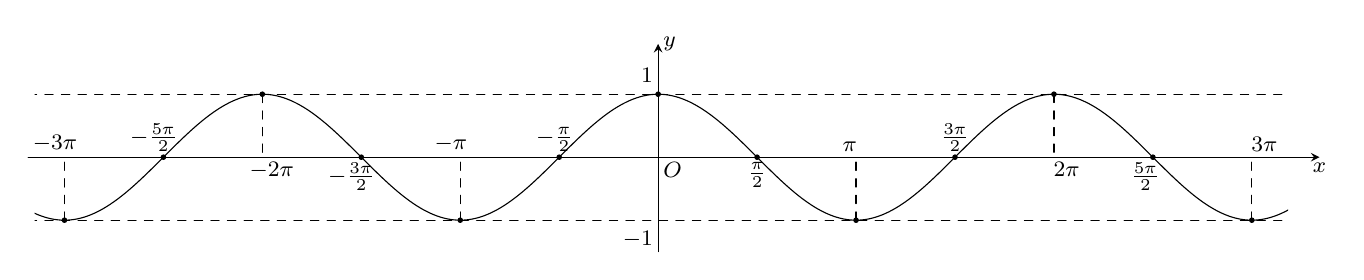
\begin{tikzpicture}[scale=0.8,>=stealth,font=\footnotesize,line join=round,line cap=round]
    \def\xmin{-10}  \def\xmax{10.5} \def\ymin{-1.5} \def\ymax{1.8}
    \draw[->]  (\xmin,0)--(\xmax,0) node [below]{$x$};
    \draw[->]  (0,\ymin)--(0,\ymax) node [right]{$y$};
    \node at (0,0) [below  right]{$O$};
    \clip (\xmin+0.1,\ymin+0.1) rectangle (\xmax-0.5,\ymax-0.1); 
     \draw[smooth,samples=400,domain=\xmin:\xmax] plot (\x,{cos (\x r)});
    \draw[dashed]  (\xmin,1)--(\xmax,1)
     (\xmin,-1)--(\xmax,-1); 
    \foreach \x  in {-3*pi,-2.5*pi,-2*pi,-1.5*pi,-pi,-0.5*pi,0}
     {\draw[fill=black] (\x,cos \x*180/pi) circle (1pt); 
     \draw[dashed] (\x,cos \x*180/pi)--(\x,0);
    \draw[fill=black] (-\x,cos  -\x*180/pi) circle (1pt);
    \draw[dashed] (-\x,cos  \x*180/pi)--(-\x,0);}
     \node at (0,1.3) [left]{$1$};
    \node at  (0,-1.3) [left]{$-1$};
    \node  at (-2*pi+0.15,0) [below]{$-2\pi$};
    \node  at (-3*pi-0.15,0) [above]{$-3\pi$};
    \node at (-2.4*pi,0)  [above left]{$-\frac{5\pi}{2}$};
    \node  at (-1.4*pi,0) [below left]{$-\frac{3\pi}{2}$};
    \node at  (-pi-0.15,0) [above]{$-\pi$};
    \node  at (-0.4*pi,0) [above left]{$-\frac{\pi}{2}$};
     \node at (0.5*pi,0) [below]{$\frac{\pi}{2}$};
     \node at (pi-0.1,0) [above]{$\pi$};
    \node  at (1.5*pi,0) [above]{$\frac{3\pi}{2}$};
     \node at (2*pi+0.2,0) [below]{$2\pi$};
    \node  at (2.5*pi+0.2,0) [below left]{$\frac{5\pi}{2}$};
    \node at (3*pi+0.2,0) [above]{$3\pi$}; 
   \end{tikzpicture}
 \end{center}
 Mỗi khẳng định sau đây  đúng hay sai?
 \choiceTF 
   {Hàm số $y=f(x)$ là hàm số tuần hoàn với chu kỳ là $\dfrac{\pi}{2}$}
  { Hàm số $y=f(x)$ là hàm số tuần hoàn  với chu kỳ là $\pi$}
  {\True Hàm số $y=f(x)$ là hàm số  tuần hoàn với chu kỳ là $2\pi$}
  {Hàm số $y=f(x)$ là hàm số tuần hoàn với chu kỳ  là $\dfrac{3\pi}{2}$}
 \loigiai{Dựa vào đồ thị ta thấy hàm số $y=f(x)$  là hàm số tuần hoàn với chu kỳ là $2\pi$.}
\end{ex}

% từ: cau-hoi/lop11/1D1_Ham_so_luong_giac_va_phuong_trinh_luong/1D1-4-7_Bang_bien_thien_va_do_thi.tex
\begin{ex}%[1D1H4-7]%[ma:2341fb27]
	Đường cong  trong hình dưới đây là đồ thị của một hàm số trong bốn hàm số được liệt kê ở bốn phương án $A,\ B,\ C,\ D$
	\begin{center}
		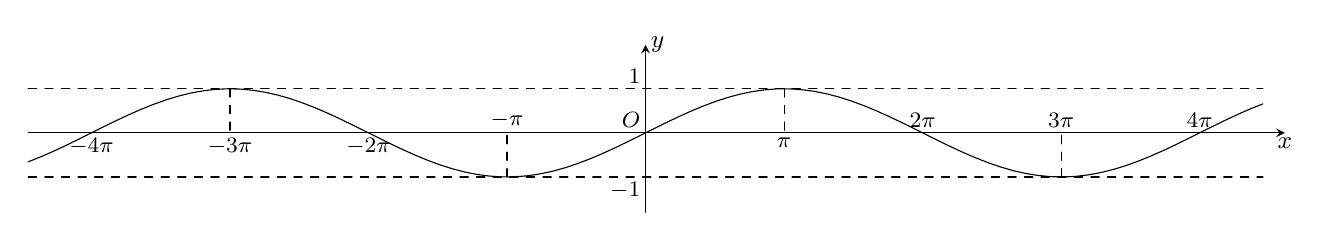
\begin{tikzpicture}[>=stealth,line join=round,line cap=round,font=\footnotesize,scale=0.56]
				\draw[->] (-14,0)  -- (14.5,0) node[below] {\small $x$};
				\draw[->] (0,-1.8) -- (0,2) node[right] {\small  $y$};
				\draw[samples=100,domain=-14:14]  plot (\x,{sin ((\x)*90/pi)});
				\draw (0,0) node [above left] {$O$}; 
				\draw (0,1) node  [above left] {$1$};
				\draw (0,-1) node  [below left] {$-1$};
				\draw (-2*pi,0)  node[below] {$-2\pi$};
				\draw (2*pi,0)  node[above] {$2\pi$};
				\draw (-4*pi,0) node[below]  {$-4\pi$};
				\draw (4*pi,0) node[above] {$4\pi$}; 
				 \draw[dashed] (-pi,-1)--(-pi,0) node[above] {$-\pi$};
				\draw[dashed] (pi,1)--(pi,0) node[below]  {$\pi$};
				\draw[dashed] (-3*pi,1)--(-3*pi,0) node[below]  {$-3\pi$};
				\draw[dashed] (3*pi,-1)--(3*pi,0) node[above] {$3\pi$}; 
				\draw[dashed]  (-14,1)--(14,1);
				 \draw[dashed] (-14,-1)--(14,-1);
			\end{tikzpicture}
	\end{center}
	Hỏi hàm số đó là hàm số nào? 
	\choice 
		{$y=\sin \dfrac{x}{2}$} 
		{$y=\cos  \dfrac{x}{2}$}
		{$y=-\cos \dfrac{x}{4}$} 
		{\True $y=\sin \left( -\dfrac{x}{2} \right)$} 
	\loigiai{ 
	Đồ thị hàm số đi qua điểm $\left( \pi;-1 \right)$ nên ta chọn hàm số $y=\sin \left( -\dfrac{x}{2} \right)$.} 
\end{ex}

% từ: cau-hoi/lop11/1D1_Ham_so_luong_giac_va_phuong_trinh_luong/1D1-4-8_Toan_thuc_te_ap_dung_ham_so_luong_giac.tex
\begin{ex}%[1D1N4-8]%[ma:e3937c7d]
	Một vật  dao động điều hòa và chuyển động theo phương trình li độ $x=5\cos \left(10\pi t+\dfrac{\pi}{6} \right)$ cm. Tìm li độ của vật tại thời điểm $t=0{,}05s$.
	\shortans{-2,5} 
	 \loigiai{
		Tại thời điểm  $t=0{,}05s$ ta có $x=5\cos \left(10\pi\cdot 0{,}05+\dfrac{\pi}{6} \right)=-2{,}5$ cm.
	 }
\end{ex}

% từ: cau-hoi/lop11/1D1_Ham_so_luong_giac_va_phuong_trinh_luong/1D1-5-2_Dieu_kien_co_nghiem.tex
\begin{ex}%[1D1V5-2]%[ma:00acbcc2]
 Cho hàm  số $y=\sin x$. Xét tính đúng-sai của các phát biểu sau:
  \choiceTF
  {Tập xác định của hàm số  $\mathbb{R}$ và tập giá trị của hàm số là $T=\left[0;1\right]$}
  {\True  Đồ thị hàm số đi qua điểm $\left(\dfrac{\pi}{4}; \dfrac{\sqrt{2}}{2} \right)$}
  {\True Đồ  thị hàm số $y=\sin x$ cắt trục hoành tại vô số điểm}
  {Đồ thị hàm số $y=\sin x$ không cắt đường  thẳng $y=2m+3$ (với $m\in \mathbb{R}$ là tham số) khi $m < \dfrac{-3}{2}$}
  \loigiai{
  \begin{itemchoice}
    \itemch Hàm số $y=\sin x$ có\\
   Tập  xác định là $\mathscr{D}=\mathbb{R}$.\\
   Tập giá trị là $T=\left[-1;1\right]$. 
   \itemch Với  $x=\dfrac{\pi}{4}$.\\
   Ta có $y=\sin x=\sin \dfrac{\pi}{4}=\dfrac{\sqrt{2}}{2}$. 
   \itemch Đồ thị  hàm số $y=\sin x$ cắt trục hoành tại vô số điểm.\\
   Hàm số $y=\sin x$ và trục hoành $y=0$.\\ 
   Phương trình hoành  độ số giao điểm của hai đồ thị là: $\sin x=0\Leftrightarrow x=k\pi \left(k\in \mathbb{Z}\right)$.\\
   Với mỗi giá trị  $k\in \mathbb{R}$ ta được một nghiệm tức là một giao điểm. Phương trình trên có vô số nghiệm.\\
   Vậy đồ thị hàm số $y=\sin x$ cắt  trục hoành tại vô số điểm.
   \itemch Phương trình hoành độ giao điểm đồ thị hàm số $y=\sin x$ và đường thẳng $y=2m+3$ là $\sin  x=2m+3$.\\
   Đồ  thị hàm số $y=\sin x$ không cắt đường thẳng $y=2m+3$ (với $m\in \mathbb{R}$ là tham số) khi phương trình $\sin x=2m+3$ vô nghiệm.\\
   Vậy ta có  $\hoac{&2m+3> 1\\&2m+3<-1}\Leftrightarrow \hoac{&m >-1\\&m <-2}\Leftrightarrow m\in \left(-\infty;-2\right)\cup \left(-1;-\infty \right)$.
  \end{itemchoice}
  }
\end{ex}

% từ: cau-hoi/lop11/1D1_Ham_so_luong_giac_va_phuong_trinh_luong/1D1-6-2_Phuong_trinh_dang_cap_bac_n_doi_voi_sinx_va_c.tex
\begin{ex}%[1D1H6-2]%[ma:5c523d86]
 Gọi $x_0$ là nghiệm dương nhỏ nhất của phương trình $3\sin^2x+2\sin x\cos x-\cos^2x=0$. Chọn khẳng  định đúng?
 \choiceTF[4] 
  {\True  $x_0\in\left(0;\dfrac{\pi}{6}\right)$}
  {$x_0\in\left(\dfrac{\pi}{4};\dfrac{\pi}{2}\right)$} 
   {\True $x_0\in\left(\dfrac{\pi}{12};\dfrac{\pi}{3}\right)$}
   {$x_0\in\left(\dfrac{\pi}{6};\dfrac{\pi}{3}\right)$}
  \loigiai{
   {\allowdisplaybreaks
  \begin{eqnarray*}
   & &3\sin^2x+2\sin  x\cos x-\cos^2x=0\\
    &\Leftrightarrow&
   (3\sin x  -\cos x)(\sin x +\cos x)=0\\
    &\Leftrightarrow&
    \hoac{&3\sin x -\cos x=0\quad(1)\\&\sin x +\cos x=0.\quad(2) }
  \end{eqnarray*}
  Nhận xét $\cos x=0$ không thỏa mãn.  Khi đó
  \begin{itemize}
   \item  $(1)\Leftrightarrow\tan x=\dfrac{1}{3}\Leftrightarrow x=\arctan\dfrac{1}{3}+k\pi, (k\in\mathbb{Z})$.
   \item $(2)\Leftrightarrow\tan  x=-1\Leftrightarrow x=-\dfrac{\pi}{4}+k\pi, (k\in\mathbb{Z})$.
  \end{itemize}
  } 
  Kết hợp  hai trường hợp ta thấy nghiệm dương nhỏ nhất của phương trình đã cho là $x_0=\arctan\dfrac{1}{3}\Rightarrow x_0\in\left(\dfrac{\pi}{12};\dfrac{\pi}{6}\right)$.
  }
\end{ex}

% từ: cau-hoi/lop11/1D2_Day_so_Cap_so_cong_Cap_so_nhan/1D2-1-1_Cau_hoi_ly_thuyet.tex
\begin{bt}%[1D2Y1-1]%[ma:7475a090]
	Viết năm số hạng đầu và số hạng thứ 100 của các dãy số $(u_n)$ có số  hạng tổng quát cho bởi:
	\begin{enumEX}[a)]{3}
		\item  $u_n=3 n-2$;
		\item $u_n=3 \cdot 2^n$; 
		\item  $u_n=\left(1+\dfrac{1}{n}\right)^{n}$.
	\end{enumEX}
	 \loigiai{
		\begin{enumEX}[a)]{1}
			\item $u_1=3\cdot 1-2=1;$ $u_2=3\cdot 2-2=4;$ $u_3=3\cdot 3-2=7;$  $u_4=3\cdot 4-2=10;$ $u_5=3\cdot 5-2=13;$ $u_{100}=3\cdot 100-2=298.$
			\item $u_1=3 \cdot 2^1=6;$ $u_2=3 \cdot 2^2=12;$ $u_3=3 \cdot 2^3=24;$ $u_4=3 \cdot 2^4=48;$ $u_5=3 \cdot 2^5=96;$  $u_{100}=3 \cdot 2^{100}.$
			\item $u_1=\left(1+\dfrac{1}{1}\right)^{1}=2$; $u_2=\left(1+\dfrac{1}{2}\right)^{2}=\dfrac{9}{4}$; $u_3=\left(1+\dfrac{1}{3}\right)^{3}=\dfrac{64}{27}$; $u_4=\left(1+\dfrac{1}{4}\right)^{4}=\dfrac{625}{256}$; $u_5=\left(1+\dfrac{1}{5}\right)^{5}=\dfrac{1296}{625}$;  $u_{100}=\left(1+\dfrac{1}{100}\right)^{100}$.
	\end{enumEX}}
\end{bt}

% từ: cau-hoi/lop11/1D2_Day_so_Cap_so_cong_Cap_so_nhan/1D2-2-2_Nhan_dien_cap_so_cong_cong_sai.tex
\begin{bt}%[1D2H2-2]%[ma:95909017]
% nguon: Archive/2024/TOAN_11_XE/TOAN_11_XE/data4/11C2/KNTT-2.3.tex #547

	Viết năm số hạng đầu của mỗi dãy số $\left(u_{n}\right)$ sau và xem nó có phải là cấp số nhân không. Nếu nó là cấp số nhân, hãy tìm công bội $q$ và viết công thức số hạng tổng quát của nó dưới dạng $u_{n}=u_{1} \cdot q^{n-1}$.
	\begin{enumEX}{2}
	\item $u_{n}=5 n$;
	\item $u_{n}=5^{n}$;
	\item $u_{1}=1$, $u_{n}=n u_{n-1}$;
	\item $u_{1}=1$, $u_{n}=5 u_{n-1}$.
	\end{enumEX}
	\loigiai{
	\begin{enumerate}
	\item Ta có $u_1=5$, $u_2=10$, $u_3=15$, $u_4=20$, $u_5=25$.\\
	Đây không là một cấp số nhân.
	\item Ta có $u_1=5$, $u_2=25$, $u_3=125$, $u_4=625$, $u_5=3125$.\\
	Đây là cấp số nhân có $q=5$, số hạng tổng quát $u_n=u_1\cdot q^{n-1}=5\cdot 5^{n-1}$, với $n\ge 2$.
	\item Ta có $u_1=1$, $u_2=2$, $u_3=6$, $u_4=12$, $u_5=60$.\\
	Đây không là một cấp số nhân.
	\item Ta có $u_1=1$, $u_2=5$, $u_3=25$, $u_4=125$, $u_5=625$.\\
	Đây là cấp số nhân có $q=5$, số hạng tổng quát $u_n=u_1\cdot q^{n-1}=1\cdot 5^{n-1}=5^{n-1}$, với $n\ge 2$.
	\end{enumerate}
	}
\end{bt}

% từ: cau-hoi/lop11/1D2_Day_so_Cap_so_cong_Cap_so_nhan/1D2-2-2_Nhan_dien_cap_so_cong_cong_sai.tex
\begin{bt}%[1D2H2-2]%[ma:601a7866]
% nguon: Archive/SP_KhoLatex/ID6_old/1K2-7.tex #3440
%[Dự án 2 - TLDH - TeamTeXHoa- Phạm Hoàng Đăng]
	Viết năm số hạng đầu của mỗi dãy số $(u_n)$ sau và xem nó có phải là cấp số nhân không. Nếu nó là cấp số nhân, hãy tìm công bội $q$ và viết công thức số hạng tổng quát của nó dưới dạng $u_n=u_1\cdot q^{n-1}$
	\begin{multicols}{2}
		\begin{enumerate}
			\item $u_n=5n$; 
			\item $u_n=5^n$;
			\item $u_1=1,u_n=nu_{n-1}$;
			\item $u_1=1,u_n=5u_{n-1}$.
		\end{enumerate}
	\end{multicols}
	\loigiai{
		\begin{enumerate}
			\item Năm số hạng đầu của dãy là $5;10;15;20;25$.\\
			Ta có $10:5=2\ne 15:10=\dfrac{3}{2}$ suy ra $(u_n)$ không phải cấp số nhân. 
			\item Năm số hạng đầu của dãy là $5;25;125;625;3125$.\\
			Ta có $u_n=5^n$ nên $u_{n+1}=5^{n+1}\Rightarrow \dfrac{u_{n+1}}{u_n}=\dfrac{5^{n+1}}{5^n}=5\,(\forall n\ge 2)$.\\
			Do đó $(u_n)$ là cấp số nhân có công bội $q=5$.\\
			Số hạng tổng quát $u_n=5\cdot {5}^{n-1}$. 
			\item Năm số hạng đầu của dãy $1;2;6;24;120$.\\
			Ta có $2:1=2\ne 6:2=3$ nên $(u_n)$ không phải là cấp số nhân.
			\item Năm số hạng đầu của dãy $1;5;25;125;625$.\\
			Ta có $u_n=5u_{n-1}$ nên $\dfrac{u_n}{u_{n-1}}=5\,(\forall n\ge 2)$.\\
			Do đó $(u_n)$ là cấp số nhân với công sai $q=5$.\\
			Số hạng tổng quát $u_n=5^{n-1}$.
		\end{enumerate}
		
	} 
\end{bt}

% từ: cau-hoi/lop11/1D2_Day_so_Cap_so_cong_Cap_so_nhan/1D2-3-3_So_hang_tong_quat_cua_cap_so_nhan.tex
\begin{ex}%[1D2V3-3]%[ma:bbd2df55]
	Cho dãy số $\left(u_n \right)$ thỏa  mãn
	$\heva{&5u_1+\sqrt{5u_1-u_2}=u_2+6 \\ &u_{n+1}=3u_n}$,  $\forall n\in \mathbb{N^*}$.
	Giá trị nhỏ nhất của $n$ để $u_n  \ge 2\cdot 3^{2\,018}$ bằng
	\choice 
		{$2\,017$} 
		 {$2\,018$}
		{\True $2\,019$} 
		 {$2\,010$}
	\loigiai{ 
		 \[\heva{&{5u_1+\sqrt{5u_1-u_2}=u_2+6\qquad(1)} \\
		 &{u_{n+1}=3u_n ,\, \forall n\in \mathbb{N}^{*}\quad\qquad\qquad (2)}
		.}\] 
		Từ $(1)$ có 
		\begin{align*}
			5u_1+\sqrt{5u_1-u_2}=u_2+6 
			&\Leftrightarrow \left(\sqrt{5u_1-u_2} \right)^2+\sqrt{5u_1-u_2}-6=0\\ 
			&\Leftrightarrow  \sqrt{5u_1-u_2}=2\Leftrightarrow 5u_1-u_2=4.
		\end{align*}
		Từ  $(2)$ có $u_{n+1}=3u_n \Rightarrow u_2=3u_1$.\\
		 Giải hệ $\heva{&{5u_1-u_2=4} \\
		&{u_2=3u_1}}$ được $u_1=2$.\\ 
		Dãy $\left(u_n \right)$ là cấp số  nhân với $\heva{&{u_1=2} \\
		&{q=3}}$  có số hạng tổng quát $u_n=2\cdot 3^{n-1}$ với $n\in \mathbb{N}^*$.\\
		\[u_n \ge  2\cdot 3^{2\,018} \Leftrightarrow 2\cdot 3^{n-1} \ge 2\cdot 3^{2\,018} \Leftrightarrow n-1\ge 2\,018\Leftrightarrow n\ge 2\,019.\]
		Vậy giá trị nhỏ nhất thỏa mãn là $2\,019$. 
	} 
\end{ex}

% từ: cau-hoi/lop11/1D2_Day_so_Cap_so_cong_Cap_so_nhan/1D2-3-4_Tim_so_hang_cu_the_trong_cap_so_nhan.tex
\begin{ex}%[1D2H3-4]%[ma:d2fdfdd7]
	Cho dãy $\left(u_n\right)$ với $u_n=\left(\dfrac{1}{2}\right)^n+1$, $\forall n\in{\mathbb{N}^*}$. Tính $S_{2\,019}=u_1+u_2+u_3+\cdots +u_{2\,019}$, ta  được kết quả
	 \choice
		 {\True $2\,020-\dfrac{1}{2^{2\,019}}$}
		 {$\dfrac{4\,039}{2}$}
		{$2\,019+\dfrac{1}{2^{2\,019}}$} 
		 {$\dfrac{6\,057}{2}$}
	 \loigiai{
		$S_{2\,019}=2\,019+\left(\dfrac{1}{2}\right)^1+\left(\dfrac{1}{2}\right)^2+\cdots +\left(\dfrac{1}{2}\right)^{2\,019}=2\,019+\dfrac{1}{2}\cdot  \dfrac{1-\left(\dfrac{1}{2}\right)^{2\,019}}{1-\dfrac{1}{2}}=2\,020-\dfrac{1}{2^{2\,019}}$.
	 }
\end{ex}

% từ: cau-hoi/lop11/1D2_Day_so_Cap_so_cong_Cap_so_nhan/1D2-3-4_Tim_so_hang_cu_the_trong_cap_so_nhan.tex
\begin{ex}%[1D2C3-4]%[ma:c13eb66b]
	Cho dãy số $(u_n)$ thỏa mãn $\heva{& 3u_1 =  \sqrt{3u_1 - u_2} + u_2 + 6 \\ & u_{n+1} = 2u_n,~\forall n \in \mathbb{N}^*}$. Tìm giá trị nhỏ nhất của $n$ để $u_n \ge 2^{2021}$.
	 \choice
		 {$2021$}
		 {$1012$}
		 {$2022$}
		{\True  $1011$}
	\loigiai{ 
		Ta có: $u_{n+1}  = 2u_n \Rightarrow \dfrac{u_{n+1}}{u_n} = 2,~\forall n \in \mathbb{N}^*$ nên dãy $(u_n)$ là cấp số nhân với công bội $q = 2$. \\
		$\Rightarrow u_2  = 2u_1$. \\
		 Mà
		\begin{eqnarray*}
			&&3u_1 = \sqrt{3u_1 - u_2} + u_2  + 6\\
			&\Leftrightarrow& 3u_1 - u_2 - \sqrt{3u_1 - u_2} - 6 = 0 \\ 
			&\Leftrightarrow& \left(\sqrt{3u_1 - u_2}\right)^2 - \sqrt{3u_1  - u_2} - 6 = 0 \\
			&\Leftrightarrow& \heva{& \sqrt{3u_1 - u_2} = 2~\text{(nhận)}\\ & \sqrt{3u_1 -  u_2} = -3~\text{(loại)}}\\
			&\Leftrightarrow & 3u_1 -  u_2 = 4.
		\end{eqnarray*}
		Từ đó ta có \[\heva{& u_2 = 2u_1 \\ & 3u_1 - u_2 = 4} \Rightarrow  u_1 = 4.\]
		$\Rightarrow (u_n)$ là cấp số nhân với công bội $q = 2, u_1 = 4$. Nên số hạng tổng quát  là \\
		$u_n = 2 \cdot 4^{n-1} = 2 \cdot  2^{2(n-1)} = 2^{2n-1},~\forall n \in \mathbb{N}^*$. \\
		$u_n \ge 2^{2021} \Leftrightarrow 2^{2n-1} \ge 2^{2021} \Leftrightarrow 2n-1 \ge 2021  \Leftrightarrow n \ge 1011$. \\
		Vậy giá trị nhỏ nhất thỏa mãn là  $1011$.
	} 
\end{ex}

% từ: cau-hoi/lop11/1D2_Day_so_Cap_so_cong_Cap_so_nhan/1D2-3-6_Tinh_tong_cua_cap_so_nhan.tex
\begin{ex}%[1D2V3-6]%[ma:86ec9391]
	Cho dãy số $\left(u_n \right)$ thỏa mãn $\heva{&5u_1+\sqrt{5u_1-u_2}=u_2+6 \\& u_{n+1}=3u_n \forall n \in \mathbb{N}^*}$. Giá trị nhỏ nhất của $n$ để $u_n \geq 2\cdot3^{2018}$ bằng bao nhiêu? 
	\shortans{2019} 
	 \loigiai{Ta có $\heva{& 5u_1 + \sqrt{5u_1 - u_2} = u_2 + 6\,(1) \\& u_{n+1} = 3u_n \forall n \in \mathbb{N}^* \,(2).}$\\
		Từ $(1)$ có $5u_1 + \sqrt{5u_1 - u_2} = u_2 + 6 \Leftrightarrow \left(\sqrt{5u_1 - u_2} \right)^2 + \sqrt{5u_1  - u_2} - 6 = 0 \Leftrightarrow 5u_1 - u_2 = 4$.\\
		Từ $(2)$ có $u_{n+1} = 3u_n \Rightarrow u_2 = 3u_1$. Giải  hệ $\heva{& 5u_1 - u_2 = 4 \\& u_2 = 3u_1}$ được $u_1 = 2$.\\
		Dãy $\left(u_n \right) $ là cấp số nhân  với $\heva{& u_1 = 2 \\& q = 3}$ có số hạng tổng quát $u_n = 2\cdot 3^{n-1}$ với $n \in \mathbb{N}^*$.\\
		Ta có $u_n \geq 2\cdot 3^{2018} \Leftrightarrow 2\cdot 3^{n-1} \geq 2\cdot 3^{2018}  \Leftrightarrow n-1 \geq 2018 \Leftrightarrow n \geq 2019$.\\
		Vậy giá  trị nhỏ nhất thỏa mãn là $2019$.
	 }
\end{ex}

% từ: cau-hoi/lop11/1D3_Gioi_han_Ham_so_lien_tuc/1D3-1-2_Phuong_phap_dat_thua_so_chung_lim_huu_han.tex
\begin{ex}%[1D3V1-2]%[ma:67130b85]
	 Cho dãy số $(u_n)$ với $u_n=\dfrac{1^2+2^2+3^2+ \cdots +n^2}{n^3+2n+7}$. Tính giới hạn của dãy số $(u_n)$.
	 \shortans{0,33}
	 \loigiai{
		Ta có kết  quả quen thuộc $1^2+2^2+3^2+\cdots +n^2=\dfrac{n(n+1)(2n+1)}{6}$.\\
		 Do đó
		$$\begin{aligned}
		\lim \dfrac{1^2+2^2+3^2+4^2+  \cdots +n^2}{n^3+2n+7}
		&=\lim  \dfrac{n(n+1)(2n+1)}{6(n^3+2n+7)} \\
		&=\lim  \dfrac{\left(1+\dfrac{1}{n}\right)\left(2+\dfrac{1}{n}\right)}{6\left(1+\dfrac{2}{n^2}+\dfrac{7}{n^3}\right)}
		 =\dfrac{1\cdot 2}{6}=\dfrac{1}{3}\approx 0{,}33.
	\end{aligned}$$
 }
\end{ex}

% từ: cau-hoi/lop11/1D3_Gioi_han_Ham_so_lien_tuc/1D3-1-2_Phuong_phap_dat_thua_so_chung_lim_huu_han.tex
\begin{ex}%[1D3V1-2]%[ma:6b0b1252]
	Cho dãy số $(u_n)$ với $u_n=\dfrac{1+2+3+ \cdots +n}{n^2+1}$. Tính giới  hạn của dãy số $(u_n)$.\\
	 \shortans{0,5}
	 \loigiai{
		Ta  có $\lim{u_n}=\lim \dfrac{1+2+3+ \cdots +n}{n^2+1}
		=\lim \dfrac{n(n+1)}{2(n^2+1)} =\dfrac{1}{2}  = 0{,}5$.
	} 
\end{ex}

% từ: cau-hoi/lop11/1D3_Gioi_han_Ham_so_lien_tuc/1D3-1-4_Gioi_han_vo_cuc.tex
\begin{ex}%[1D3H1-4]%[ma:23f04170]
	Cho dãy số $\left(u_n\right)$ xác định $u_{1}=0$, $u_{2}=1$, $u_{n+1}=2$, $u_n-u_{n-1}+2$  với mọi $n \geq 2$. Tìm giới hạn của dãy số $\left(u_n\right)$.
	\loigiai{Ta có $u_{1}=0, u_{2}=1, u_{3}=4, u_{4}=9$.\\ 
		Bằng phương pháp quy nạp, dễ dàng chứng minh được $u_n=(n-1)^{2}$ với mọi $n  \geq 1$.\\ Do đó $\lim u_n=\lim (n-1)^{2}=+\infty$.
	 }
\end{ex}

% từ: cau-hoi/lop11/1D6_Ham_so_mu_va_ham_so_logarit/1D6-1-4_So_sanh_cac_luy_thua.tex
\begin{bt}%[1D6H1-4]%[ma:2de31430]
% nguon: Archive/2024/TOAN_11_XE/TOAN_11_XE/data4/11C6/KNTT-6.1.tex #969
%[TeX hóa CD 11]%[Nhật Thiện]
	Viết các số sau theo thứ tự tăng dần
	\begin{listEX}[2]
		\item $1^{1{,}5}$; $3^{-1}$; $\left(\dfrac{1}{2}\right)^{-2}$;
		\item $2\,022^0$; $\left(\dfrac{4}{5}\right)^{-1}$; $5^{\frac{1}{2}}$.
	\end{listEX}
	\loigiai{
		\begin{enumerate}
			\item Ta có $1^{1{,}5}=1$; $3^{-1}=\dfrac{1}{3}$; $\left(\dfrac{1}{2}\right)^{-2}=4$.\\
			Sắp xếp theo thứ tự tăng dần sẽ là $3^{-1}$; $1^{1{,}5}$; $\left(\dfrac{1}{2}\right)^{-2}$.
			\item $2\,022^0=1$; $\left(\dfrac{4}{5}\right)^{-1}=\dfrac{5}{4}$; $5^{\frac{1}{2}}=\sqrt{5}$.\\
			Sắp xếp theo thứ tự tăng dần sẽ là $2\,022^0$; $\left(\dfrac{4}{5}\right)^{-1}$; $5^{\frac{1}{2}}$.
		\end{enumerate}
	}
\end{bt}

% từ: cau-hoi/lop11/1D6_Ham_so_mu_va_ham_so_logarit/1D6-4-1_Dieu_kien_co_nghiem.tex
\begin{ex}%[1D6V4-1]%[ma:7e218c07]
	Tất cả các giá trị của tham số $m$ để  phương trình $3^{x^2+1}=m-1$ có nghiệm là
	 \choice
		{\True  $m\geq 4$}
		 {$m>4$}
		 {$m>1$}
		{$m\geq  1$}
	 \loigiai{
		Ta có $3^{x^2} \ge 3^0 \Leftrightarrow 3^{x^2+1} \ge 3$. \\ 
		Phương trình $3^{x^2+1}=m-1$  có nghiệm khi và chỉ khi $m-1 \ge 3 \Leftrightarrow m \ge 4$.
	 }
\end{ex}

% từ: cau-hoi/lop11/1D6_Ham_so_mu_va_ham_so_logarit/1D6-4-3_Bat_phuong_trinh_mu_logarit_co_ban.tex
\begin{ex}%[1D6H4-3]%[ma:f453da9e]
	Giải  bất phương trình sau $3^{x^{2}-4x+5} > \dfrac{1}{9}$.
	\loigiai{Ta  có
		\begin{eqnarray*}
			3^{x^2-4x+5} > \dfrac{1}{9} \Leftrightarrow 3^{x^2-4x+5} > 3^{-2} \Leftrightarrow x^2-4x+5 >-2 ~(\text{do}~3 > 1)\Leftrightarrow x^2-4x+7 > 0\Leftrightarrow x\in  \mathbb{R}.
		\end{eqnarray*}
	Vậy nghiệm của bất phương  trình là $x\in \mathbb{R}$.}
\end{ex}

% từ: cau-hoi/lop11/1D6_Ham_so_mu_va_ham_so_logarit/1D6-4-4_Phuong_trinh_mu_logarit_dua_ve_cung_co_so.tex
\begin{ex}%[1D6H4-4]%[ma:369e3a99]
	Giải bất phương trình $3^{x^3-4x+5}>\dfrac{1}{9}$. 
	\loigiai{ 
		 Ta có
		\begin{eqnarray*}
			3^{x^3-4x+5}>\dfrac{1}{9}&\Leftrightarrow&3^{x^3-4x+5}>3^{-2}\\ 
			 &\Leftrightarrow& x^2-4x+5>-2 (\text{ do} 3>1)\\
			 &\Leftrightarrow& x^2-4x+7>0\\
			&\Leftrightarrow& x\in\mathbb{R}. 
		\end{eqnarray*}
		Vậy  nghiệm của bất phương trình là $x\in\mathbb{R}$.
	 }
\end{ex}

% từ: cau-hoi/lop11/1D6_Ham_so_mu_va_ham_so_logarit/1D6-4-4_Phuong_trinh_mu_logarit_dua_ve_cung_co_so.tex
\begin{bt}%[1D6H4-4]%[ma:55183975]
% nguon: Archive/SP_SauLuoi_2024-2025/Sp_GHKII/data/GHKII/1-TN-TL-THPT-PhanDinhPhung-HaNoi-GHKII-NH24-25.tex #270
%[Dự án đề KT GKII Khối 11 NH24-25-Dot 9-Tư Đô Nguyên]%[THPT Phan Đình Phùng - Hà Nội]
	Giải phương trình $\left(\dfrac{1}{3}\right)^x=3^{1+2x}$.
	\loigiai{
		Ta có $\left(\dfrac{1}{3} \right)^x = 3^{-x}$.\\
		Do đó $3^{-x} = 3^{1+2x} \Leftrightarrow -x = 1+2x \Leftrightarrow -3x=1 \Leftrightarrow x=-\dfrac{1}{3}$.\\
		Vậy $x=-\dfrac{1}{3}$ là nghiệm duy nhất.
	}
\end{bt}

% từ: cau-hoi/lop11/1D7_Dao_ham/1D7-1-1_Tinh_dao_ham_bang_dinh_nghia.tex
\begin{ex}%[1D7V1-1]%[ma:4c99875b]
	Cho hàm số $f(x)=\heva{& \dfrac{3-\sqrt{4-x}}{4}&& \text{khi  } x\ne 0\\&\dfrac{1}{4}&& \text{khi } x=0}$. Tính $f'(0)$.
	\choice 
		{Không  tồn tại}
		 {\True $f'(0)=\dfrac{1}{16}$}
		 {$f'(0)=\dfrac{1}{4}$}
		 {$f'(0)=\dfrac{1}{32}$}
	\loigiai{Ta có \begin{align*}
		\lim\limits_{x\to 0}\dfrac{f(x)-f(0)}{x-0}&=\lim\limits_{x\to 0}\dfrac{\dfrac{3-\sqrt{4-x}}{4}-\dfrac{1}{4}}{x}=\lim\limits_{x\to 0}\dfrac{2-\sqrt{4-x}}{4x}=\lim\limits_{x\to 0}\dfrac{4-(4-x)}{4x\left(2+\sqrt{4-x}\right)}\\ 
		&=\lim\limits_{x\to 0}\dfrac{1}{4\left(2+\sqrt{4-x}\right)}=\dfrac{1}{16}. 
	\end{align*}
	 Vậy $f'(0)=\dfrac{1}{16}$.
} 
\end{ex}

% từ: cau-hoi/lop11/1D7_Dao_ham/1D7-1-4_Y_nghia_Vat_ly_cua_dao_ham.tex
\begin{ex}%[1D7H1-4]%[ma:4c971407]
	Một chất điểm chuyển động  có phương trình chuyển động là $S(t)=\dfrac{1}{3}t^{3}-2t^{2}+3t-1$ (t được tính bằng giây, s tính bằng mét). Vận tốc tức thời của chất điểm tại thời điểm $t=4$ là
	\choice 
		 {$6$ (m/s)}
		{$4$ (m/s)} 
		{$5$  (m/s)}
		{\True $3$ (m/s)} 
	 \loigiai{
		\begin{itemize}
			 \item Ta có $v(t)=S'(t)=t^{2}-4t+3$.
			\item Vận tốc tức  thời của chất điểm tại thời điểm $t=4$ là $v(4) = 4^2-4(4)+3=3$ (m/s).
		\end{itemize}
	} 
\end{ex}

% từ: cau-hoi/lop11/1D7_Dao_ham/1D7-1-4_Y_nghia_Vat_ly_cua_dao_ham.tex
\begin{ex}%[1D7H1-4]%[ma:c66b28f2]
	Cho chuyển động được xác định  bởi phương trình $s=2t^{3}+6t^{2}-t$, trong đó $t$ được tính bằng giây và $s$ được tính bằng mét. Vận tốc tức thời của chuyển động tại thời điểm $t=3$ s là
	\choice 
		{\True $89$  m/s}
		{$105$  m/s}
		{$48$ m/s} 
		{$20$  m/s}
	 \loigiai{
		\begin{itemize}
			 \item Ta có $v(t)=s'(t)=6t^{2}+12t-1$.
			\item Vận tốc tức  thời của chuyển động khi $t=3$ s là $v(3)=6 \cdot 3^{2}+12 \cdot 3-1=89$ (m/s).
		\end{itemize}
	 }
\end{ex}

% từ: cau-hoi/lop11/1D7_Dao_ham/1D7-1-4_Y_nghia_Vat_ly_cua_dao_ham.tex
\begin{ex}%[1D7C1-4]%[ma:29dad855]
	\immini  {
	Một vật chuyển  động trong $1$ giờ với vận tốc $v$ phụ thuộc vào thời gian $t$ có đồ thị vận tốc như hình bên. Trong khoảng thời gian $1$ giờ kể từ khi bắt đầu chuyển động, đồ thị đó là một phần của đường parabol có đỉnh $I\left(\dfrac{1}{2};8\right)$ và trục đối xứng song song với trục tung. Tính gia tốc của vật lúc $t=0{,}25$ (h).
	 \choice
		{\True $16$  (km/h$^2$)}
		{$-16$  (km/h$^2$)}
		{$8$ (km/h$^2$)} 
		 {$-8$ (km/h$^2$)}
		} 
		 {
		\begin{tikzpicture}[transform shape]
				 \draw[-stealth] (-1,0)--(3,0) node[below]{$t$};
				\draw[-stealth] (0,-1)--(0,9) node [right]  {$v$};
				\draw[smooth] plot[domain=0:1]  (\x,{-32*(\x-0.5)^2+8});
				 \draw[dashed]
					(0,0) node[below left] {$O$} 
					(1,0) node[below]  {$1$}
					(.5,0)  node[below]{$\dfrac{1}{2}$}|-(0,8) node [left] {$8$};
			\end{tikzpicture}
		 }
	 \loigiai{
		\begin{itemize}
			\item Dựa vào đồ thị của hàm số, ta  suy ra $v(t)=a\cdot\left(x-\dfrac{1}{2}\right)^2+8$.
			 \item $v(1)=0\Leftrightarrow a\cdot\left(1-\dfrac{1}{2}\right)^2+8=0\Leftrightarrow a=-32$.
			\item Gia  tốc vật là $a(t)=v'(t)=-64\cdot\left(x-\dfrac{1}{2}\right)$.
			\item Lúc $t=0{,}25$ (h) thì gia tốc là $a(0{,}25)=-64\cdot\left(0{,}25-\dfrac{1}{2}\right)=16$  (km/h$^2$).
		\end{itemize}
	} 
\end{ex}

% từ: cau-hoi/lop11/1D7_Dao_ham/1D7-1-5_Toan_thuc_te_khac_ap_dung_dinh_nghia_dao_ham.tex
\begin{ex}%[1D7V1-5]%[ma:8d72a454]
	Một chất điểm chuyển động theo quy luật $s(t)=-t^3+6t^2$ với $t$ là thời gian  tính từ lúc bắt đầu chuyển động, $s(t)$ là quãng đường đi được trong khoảng thời gian $t$. Tính thời điểm $t$ tại đó vận tốc đạt giá trị lớn nhất.
	 \shortans{2}
	\loigiai{Điều kiện $t>0$.\\ 
	Vận tốc của chất điểm là $v(t)=s'(t)=-3t^2+12t=-3(t-2)^2+12\leq  12$.\\
	Dấu \rq\rq =\rq\rq\, xảy ra khi  và chỉ khi $ t=2 $.\\
	Vậy vận tốc chuyển động của  chất điểm đạt giá trị lớn nhất khi $t=2$.
	} 
\end{ex}

% từ: cau-hoi/lop11/1D7_Dao_ham/1D7-1-5_Toan_thuc_te_khac_ap_dung_dinh_nghia_dao_ham.tex
\begin{ex}%[1D7C1-5]%[1D5B3-3]%[ma:6cc63e53]
	\immini 
	 {
	Một vật gắn trên lò xo chuyển động theo phương ngang trên mặt phẳng nhẵn như hình bên. Phương trình chuyển động của vật được cho bởi $x=8\sin\left(\sqrt{2}\pi t+\dfrac{\pi}{3}\right)$, với $t$ tính bằng giây và $x$ tính bằng centimet. Tìm vận tốc và gia tốc của vật tại thời điểm $t=5$ giây (làm tròn đến chữ số  thập phân thứ nhất). Vật chuyển động theo hướng nào tại thời điểm đó?
	 }
	 {
	\begin{tikzpicture}[line cap=round,line join=round,>=triangle 45,x=1cm,y=1cm]
			 \draw [smooth,domain=3.13:15*pi,scale=0.1,samples=100] plot (\x,{4*sin (\x r)+7});
			 \fill [pattern = north east lines] (-0.2,0) rectangle (0,4);
			\draw[fill=gray]  (4.9,1.5)--(5.5,1.5)--(5.5,0)--(4.9,0)--cycle;
			\draw[->](0,0)--(6,0); 
			 \draw[->] (2.5,2.5)--(2.5,1.2);
			\draw (0,0) -- (0,4) 
				(2.5,0.1)--(2.5,-0.1) 
				(5.2,0.1)--(5.2,-0.1); 
			\draw (2.5,3) node {vị trí cân  bằng}
				(2.5,-0.3) node  {$O$}
				(5.2,-0.3) node  {$x$}
				(6,-0.3)  node {$x$}
				(3,-1) node  {Hình 9.1};
			 \draw (0,0.7)--(0.3,0.7)
				(4.72,0.7)--(4.9,0.7); 
		\end{tikzpicture}
	} 
	\shortans{151} 
	 \loigiai{
		Vận tốc và gia  tốc của vật tại thời điểm $t$ là
		\begin{itemize}
			 \item $v(t)=x'(t)=8\pi\sqrt{2}\cos\left(\sqrt{2}\pi t+\dfrac{\pi}{3}\right)$;
			 \item $a(t)=v'(t)=-16\pi^2\sin\left(\sqrt{2}\pi t+\dfrac{\pi}{3}\right)$.
		\end{itemize}
		Tại thời điểm $t=5$, vận tốc của vật là $v(5)=8\pi\sqrt{2}\cos\left(\sqrt{2}\pi \cdot 5+\dfrac{\pi}{3}\right)\approx -10{,}5$ cm/s.\\ 
		Gia tốc của vật  là $a(5)=-16\pi^2\sin\left(\sqrt{2}\pi \cdot 5+\dfrac{\pi}{3}\right)\approx 150{,}8$ cm/s$^2$.
	} 
\end{ex}

% từ: cau-hoi/lop11/1D7_Dao_ham/1D7-2-1_Tinh_dao_ham.tex
\begin{ex}%[1D7H2-1]%[ma:7e81144a]
	Cho hàm số $y=x^3+mx^2+3x-5$ với $m$ là tham số. Tìm tập hợp $M$  tất cả các giá trị của $m$ để $y'=0$ có hai nghiệm phân biệt.
	 \choice
		{$M=(-3;3)$} 
		{$M=(-\infty;-3]\cup[3;+\infty)$} 
		 {$M=\mathbb{R}$}
		{\True  $M=(-\infty;-3)\cup(3;+\infty)$}
	 \loigiai{
		Ta có $y=x^3+mx^2+3x-5$ nên $y'=3x^2+2mx+3$.  Do đó,\\
		 $y'=0$ có hai nghiệm phân biệt khi và chỉ khi
		\begin{align*}
			\Delta'>0\Leftrightarrow m^2-9>0\Leftrightarrow \hoac{&m<-3\\  &m>3.}
		\end{align*}
		Vậy  $M=(-\infty;-3)\cup(3;+\infty)$.
	 }
\end{ex}

% từ: cau-hoi/lop11/1D7_Dao_ham/1D7-2-1_Tinh_dao_ham.tex
\begin{ex}%[1D7V2-1]%[ma:fb0b0593]
	Cho hàm số $f(x)=\sqrt{x^2-2x}$. Tập nghiệm $S$  của bất phương trình $f'(x)\geq f(x)$ có bao nhiêu giá trị nguyên?
	 \choice
		 {$1$}
		{$2$} 
		 {\True $0$}
		{$3$} 
	 \loigiai{
		Tập xác định của hàm số là $\mathscr{D}=(-\infty;0]\cup[2;+\infty)$.\\ 
		Ta có $f'(x)=\dfrac{(x^2-2x)’}{2\sqrt{x^2-2x}}=\dfrac{x-1}{\sqrt{x^2-2x}}$, $\forall  x\in(-\infty;0)\cup(2;+\infty)$.\\
		Do đó, với $x\in(-\infty;0)\cup(2;+\infty)$,  ta có\allowdisplaybreaks
		\begin{align*}
			f'(x)\geq  f(x)&\Leftrightarrow\dfrac{x-1}{\sqrt{x^2-2x}}\geq\sqrt{x^2-2x}\\
			&\Leftrightarrow  x-1\geq x^2-2x\\
			&\Leftrightarrow x^2-3x+1\leq0\\ 
			&\Leftrightarrow\dfrac{3-\sqrt{5}}{2}\leq  x\leq\dfrac{3+\sqrt{5}}{2}.
		\end{align*}
		Kết hợp với điều kiện $x\in(-\infty;0)\cup(2;+\infty)$, ta được  $S=\left(2;\dfrac{3+\sqrt{5}}{2}\right]$.\\
		Ta có $\dfrac{3+\sqrt{5}}{2}\approx 2{,}6$. Do đó, trên khoảng $\left(2;\dfrac{3+\sqrt{5}}{2}\right]$ không có số nguyên  nào.\\
		Vậy tập nghiệm $S$ của bất phương trình $f'(x)\geq f(x)$ không có  giá trị nguyên nào.
	 }
\end{ex}

% từ: cau-hoi/lop11/1D7_Dao_ham/1D7-2-1_Tinh_dao_ham.tex
\begin{ex}%[1D7H2-1]%[ma:3c0fb340]
 Cho hàm số $y=f(x)=2\sin 3x+\cos 2x$. Xét tính đúng sai các mệnh  đề sau
 \choiceTF 
  {Hàm  số đã cho là hàm số chẵn}
  {\True Hàm số  tuần hoàn với chu kì $T=2\pi$}
   {$f(x)=f\left(\dfrac{\pi}{2}-x\right)$}
  {\True Đạo hàm của hàm số đã  cho là $y'=6\cos 3x-2\sin 2x$}
 \loigiai{ 
  \begin{itemchoice}
   \itemch Tập xác định $\mathscr{D}=\mathbb{R}$.\\ 
   Xét $f(-x)=2\sin  (-3x)+\cos (-2x)=-2\sin 3x+\cos 2x$.\\
    Suy ra $f(-x)\ne f(x)$. \\
   Vậy hàm số đã cho không phải hàm  số chẵn. Mệnh đề đã cho sai.
   \itemch Ta có $\sin 3x=\sin (3x+2\pi)$ và  $\cos 2x=\cos (2x+2\pi)$.\\
   Vậy hàm số đã  cho tuần hoàn với chu kì $T=2\pi$. Mệnh đề đã cho đúng.
    \itemch Ta có
   \begin{eqnarray*}
    f\left(\dfrac{\pi}{2}-x\right)&=&2\sin \left[3\left(\dfrac{\pi}{2}-x\right)\right]+\cos \left[2\left(\dfrac{\pi}{2}-x\right)\right]=2\sin  \left(\dfrac{3\pi}{2}-3x\right)+\cos (\pi-2x)\\
    &=&-2\sin \left(\dfrac{\pi}{2}-3x\right)-\cos  2x\\
     &=&-2\cos 3x-\cos 2x\ne f(x).
   \end{eqnarray*}
   Vậy  mệnh đề đã cho sai.
   \itemch Ta có $y'=2{(\sin  3x)}'+{(\cos 2x)}'=2\cos 3x\cdot(3x)'-\sin 2x\cdot(2x)'=6\cos 3x-2\sin 2x$.\\
   Mệnh đề đã  cho đúng.
  \end{itemchoice}
  }
\end{ex}

% từ: cau-hoi/lop11/1D7_Dao_ham/1D7-2-1_Tinh_dao_ham.tex
\begin{ex}%[1D7H2-1]%[ma:923ea6e8]
	Tìm đạo  hàm của các hàm số sau
	\begin{enumEX}{2}
		 \item $y=5\sin x-3\cos x$;
		 \item $y=\sin\left(x^2-3x+2\right)$;
		 \item $ y=\sqrt{1+2\tan x}$;
		\item $y=\tan 3x-\cot  3x$.
	\end{enumEX}
	 \loigiai{
		\begin{enumerate}
			\item Ta có $y'=5\cos x+3\sin  x$.
			\item  Ta có $y'=\left(x^2-3x+2\right)'\cdot \cos\left(x^2-3x+2\right)$ $=\left(2x-3\right)\cdot \cos \left(x^2-3x+2\right)$.
			\item Ta  có $y'=\dfrac{\left(2\tan x\right)'}{2\sqrt{1+2\tan x}}$ $=\dfrac{\dfrac{2}{\cos^2x}}{2\sqrt{1+2\tan x}}$ $=\dfrac{1}{\cos^2x\cdot \sqrt{1+2\tan x}}$.
			\item Ta có thể làm bằng  hai cách sau
			\begin{itemize}
				\item \textbf{Cách 1.} Ta có  ngay
				 $$y'=\dfrac{3}{\cos^23x}+\dfrac{3}{\sin^23x}=\dfrac{3}{\sin^23x\cdot \cos^23x} =\dfrac{3}{\tfrac{1}{4}{\sin^2}6x}=\dfrac{12}{\sin^26x}.$$
				\item \textbf{Cách 2.} Ta biến  đổi
				$$y=\dfrac{\sin 3x}{\cos 3x}-\dfrac{\cos  3x}{\sin 3x}=\dfrac{\sin^23x-\cos^23x}{\cos 3x\cdot \sin 3x}=-\dfrac{2\cos 6x}{\sin 6x}=-2\cot 6x.$$
				Vậy  $y'=\dfrac{12}{\sin^26x}$.
			\end{itemize}
		\end{enumerate}
	 }
\end{ex}

% từ: cau-hoi/lop11/1D7_Dao_ham/1D7-3-1_Tinh_dao_ham_cap_hai.tex
\begin{ex}%[1D7H3-1]%[ma:d6472d3c]
	Cho hàm số $f(x)=\sin^2x$, với mọi $x\in  \mathbb{R}$ ta có $f"(x)$ bằng
	\choice 
		{$f"(x)=2\cos x$} 
		 {$f"(x)=2\sin 2x$}
		 {$f"(x)=\cos 2x$}
		{\True $f"(x)=2\cos  2x$}
	\loigiai{ 
		Ta có: $f'(x)=2\sin x\cos x=\sin 2x$; $f"(x)=2\cos 2x$. 
	} 
\end{ex}

% từ: cau-hoi/lop11/1D7_Dao_ham/1D7-3-1_Tinh_dao_ham_cap_hai.tex
\begin{ex}%[1D7H3-1]%[ma:8bdc33e8]
	Cho hàm  số $f(x)=\dfrac{1}{12}x^4-\dfrac{5}{6}x^3+3x^2+3x$.
	\choiceTF 
		{$f''(1)=0$} 
		{\True  $f''(3)=0$}
		{\True $f''(x) < 0\Leftrightarrow 2< x < 3$} 
		{Đồ thị hàm số $y=f''(x)$ có trục  đối xứng là đường thẳng $x=5$}
	 \loigiai{
		Ta  có $f'(x)=\dfrac{1}{3}x^3-\dfrac{5}{2}x^2+6x+3$ và $f''(x)=x^2-5x+6$.
		\begin{itemchoice}
			\itemch Ta có  $f''(1)=1^2-5\cdot 1+6=2$.
			\itemch Ta có $f''(3)=0$. 
			\itemch Ta  có $f''(x)=x^2-5x+6<0\Leftrightarrow 2<x<3$.
			\itemch Đồ thị hàm số  $y=f''(x)$ là một parabol có trục đối xứng là $x=-\dfrac{b}{2a}=\dfrac{5}{2}$.
		\end{itemchoice}
	} 
\end{ex}

% từ: cau-hoi/lop11/1D7_Dao_ham/1D7-3-1_Tinh_dao_ham_cap_hai.tex
\begin{bt}%[1D7N3-1]%[ma:b8bdef1d]
% nguon: Archive/2024/TOAN_11_XE/TOAN_11_XE/data4/11C9/KNTT-9.3.tex #1310

	Tính đạo hàm cấp hai của các hàm số:
	\begin{multicols}{2}
		\begin{enumerate}
			\item $y=3x^2+5x+1$;
			\item $y=\sin x$.
		\end{enumerate}
	\end{multicols}
	\loigiai{
		\begin{enumerate}
			\item $y=3x^2+5x+1$.\\
			$y'=\left(3x^2+5x+1\right)'=6x+5$, $y^{\prime\prime} =\left(6x+5\right)'=6$.
			\item $y=\sin x$.\\
			$y'=\left(\sin x\right)'=\cos x$, $y^{\prime\prime} =\left(\cos x\right)'=-\sin x$.
		\end{enumerate}
	}
\end{bt}

% từ: cau-hoi/lop11/1D7_Dao_ham/1D7-3-1_Tinh_dao_ham_cap_hai.tex
\begin{bt}%[1D7H3-1]%[ma:533c69f3]
% nguon: Archive/2024/TOAN_11_XE/TOAN_11_XE/data4/11C9/KNTT-9.3.tex #1313

	Tính đạo hàm cấp hai của các hàm số sau:
	\begin{multicols}{2}
		\begin{enumerate}
			\item $y=x^2-x$;
			\item $y=\cos x$.
		\end{enumerate}
	\end{multicols}	
	\loigiai{\begin{enumerate}
			\item $y=x^2-x$.\\
			$y'=(x^2-x)'=2x-1$, $y^{\prime\prime}=(2x-1)'=2$.
			\item $y=\cos x$.\\
			$y'=(\cos x)'=-\sin x$, $y^{\prime\prime}=(-\sin x)'=-(\sin x)'=-\cos x$.
		\end{enumerate}
	}
\end{bt}

% từ: cau-hoi/lop11/1D9_Xac_suat/1D9-1-2_Xac_dinh_va_dem_so_phan_tu_bien_co_giao.tex
\begin{ex}%[1D9N1-2]%[ma:9452c630]
	Một hộp đựng 25 tấm thẻ cùng loại được đánh số từ 1 đến 25. Rút ngẫu nhiên một tấm thẻ trong hộp. Xét các biến số P: \lq\lq Số ghi  trên tấm thẻ là số chia hết cho 4\rq\rq \, và Q: \lq\lq Số ghi trên tấm thẻ là số chia hết cho 6\rq\rq. Nội dung của biến cố giao PQ là gì?
	\choice 
		 {$\left\{3;6;9;12;15;18;24\right\}$}
		 {$\{1;2;4\}$}
		 {$\left\{12;16;20;24\right\}$}
		 {\True $\{12;24\}$}
	 \loigiai{
	Bội chung của  $4$ và $6$ là $\left\{12;24\right\}$.}
\end{ex}

% từ: cau-hoi/lop11/1D9_Xac_suat/1D9-1-3_Cong_thuc_nhan_xac_suat_cho_2_bien_co_doc_lap.tex
\begin{ex}%[1D9H1-3]%[ma:2837b482]
	Một hộp chứa $22$ tấm thẻ cùng loại được đánh số lần lượt từ $1$ đến $22$. Chọn ra ngẫu nhiên $1$ thẻ từ hộp. Gọi $A$ là biến cố \lq\lq Số ghi trên thẻ được chọn chia hết cho $2$\rq\rq,  $B$ là biến cố \lq\lq Số ghi trên thẻ được chọn chia hết cho $3$\rq\rq. Xác suất của biến cố $AB$ bằng
	 \choice
		{\True  $\dfrac{3}{22}$}
		 {$\dfrac{7}{22}$}
		{$\dfrac{1}{2}$} 
		{$\dfrac{7}{44}$} 
	 \loigiai{
		Không gian mẫu $\Omega=\left\{1;\; 2;\; 3;\;...;\; 22\right\}$,  suy ra $n\left(\Omega \right)=22$.\\
		Ta  có $A$ là biến cố \lq\lq Số ghi trên thẻ được chọn chia hết cho $2$\rq\rq \, $\Rightarrow A=\left\{2;\; 4;\; 6;\;...;\; 22\right\}$.\\
		$B$ là biến cố  \lq\lq Số ghi trên thẻ được chọn chia hết cho $3$\rq\rq \, $\Rightarrow B=\left\{3;\; 6;\; 9;\; 12;\; 15;\; 18;\; 21\right\}$.\\
		 Ta cũng có $A\cap B=\left\{6;\; 12;\; 18\right\}$, suy ra $\mathrm{P}(AB)=\dfrac{3}{22}$.
	} 
\end{ex}

% từ: cau-hoi/lop11/1H4_Duong_thang_mat_phang_Quan_he_song_song/1H4-4-1_Cau_hoi_ly_thuyet.tex
\begin{ex}%[1H4N4-1]%[ma:cd3f8656]
 Cho hình chóp $S.ABCD$ có $ABCD$ là hình  thang với $BC$ là đáy bé.
 \choiceTF 
  {\True Giao tuyến của $2$ mặt phẳng $(SAD)$ và $(SAB)$ là $SA$} 
   {Giao tuyến của $2$ mặt phẳng $(SAD)$ và $(SBC)$ là đường thẳng $SO$, với $O=AC \cap BD$}
  {\True Giao tuyến của $2$ mặt phẳng $(SAC)$ và $(SBD)$  là đường thẳng $SO$, với $O=AC \cap BD$}
  {\True Giao điểm của $CD$ với mặt phẳng $(SAB)$ là $I$  với $I=CD \cap AB$}
  \loigiai{
  \begin{center}
   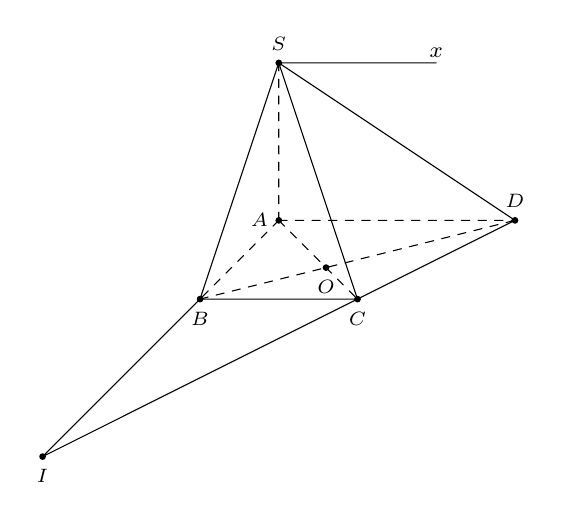
\begin{tikzpicture}[line join = round,line cap = round,>=stealth,font=\footnotesize,scale=1]
      \foreach \x/\y/\t in {0/0/A,3/0/D,-1/-1/B,1/-1/C,0/2/S,2/2/x}{
      \path (\x,\y) coordinate (\t); 
     } 
      \path
      (intersection of A--C  and B--D) coordinate (O)
      (intersection of D--C and B--A) coordinate  (I);
      \draw[dashed] (A)--(S)
      (A)--(B) 
       (A)--(D)
       (A)--(C)
       (B)--(D);
     \draw  (S)--(B)
       (S)--(C)
       (S)--(D)
      (B)--(C) 
      (C)--(D) 
       (S)--(x) node[above]{$x$}
      (B)--(I)--(C); 
     \foreach  \t/\g in {A/180,B/-90,C/-90,D/90,S/90,O/-90,I/-90}{
      \draw[fill=black] (\t) circle (1pt) node[shift={(\g:7pt)},font=\scriptsize]{$ \t  $};
     } 
    \end{tikzpicture}
  \end{center}
  \begin{itemchoice}
    \itemch{\bf Đúng.}\\
   Ta  có giao tuyến của $2$ mặt phẳng $(SAD)$ và $(SAB)$ là $SA$.
   \itemch{\bf  Sai.}\\
   Ta có $\heva{& AD\in (SAD) \\ & BC\in (SBC)\\ & S\in (SAD)\cap  (SBC)\\ & AD\parallel BC}\Rightarrow (SBC)\cap (SAD)=Sx\parallel AD\parallel BC$.
   \itemch{\bf Đúng.}\\ 
    Ta có giao tuyến của $2$ mặt phẳng $(SAC)$ và $(SBD)$ là đường thẳng $SO$, với $O=AC \cap BD$.
   \itemch{\bf  Đúng.}\\
   Vì $I=CD \cap AB$ nên giao điểm của $CD$ với mặt phẳng $(SAB)$  là $I$.
  \end{itemchoice}
 } 
\end{ex}

% từ: cau-hoi/lop11/1H4_Duong_thang_mat_phang_Quan_he_song_song/1H4-6-2_Hinh_bieu_dien_cua_mot_hinh_khong_gian.tex
\begin{bt}%[1H4N6-2]%[ma:e7842efc]
% nguon: Archive/2024/SP-K10-K11-LyVanHoang_TVN-023/K11-C4-HHKG-QHSS/data/Bai6-Phepchieusongsong.tex #2368
[CD]
	Trong các {\it Hình a, b, c}, hình nào biểu diễn hình lập phương?
	\begin{center}
		\begin{tikzpicture}[scale=1, font=\footnotesize, line join=round, line cap=round,>=stealth]
			\begin{scope}
				\path (0,2) coordinate (h) (0,0)coordinate (B) (2,0) coordinate (C) (1,1) coordinate (D) ($(B)+(D)-(C)$) coordinate (A);
				\foreach \p in {A,B,C,D}\path ($(\p)+(h)$) coordinate (\p');
				\draw (A')--(A)--(B)--(C)--(C')--(D')--cycle (A')--(B')--(B) (B')--(C');
				\draw[dashed] (A)--(D)--(C) (D)--(D');
				\draw ($(B)!0.4!(C)+(0,-0.5)$) node[]{$a)$};
			\end{scope}
			\begin{scope}[xshift=5cm]
				\path (0,2) coordinate (h) (0,0)coordinate (B) (2,0) coordinate (C) (2.8,1) coordinate (D) ($(B)+(D)-(C)$) coordinate (A);
				\foreach \p in {A,B,C}\path ($(\p)+(h)$) coordinate (\p');
				\path (C')--++(50:0.7) coordinate (D');
				\draw (A')--(B')--(B)--(C)--(D)--(D')--cycle (B')--(C')--(D') (C)--(C');
				\draw[dashed] (B)--(A)--(D) (A)--(A');
				\draw ($(B)!0.6!(C)+(0,-0.5)$) node[]{$b)$};
			\end{scope}
			\begin{scope}[xshift=10cm]
				\path (0,3) coordinate (h) (0,0)coordinate (B) (3,0) coordinate (C);
				\foreach \p in {B,C}\path ($(\p)+(h)$) coordinate (\p');
				\draw (B)--(C)--(C')--(B')--cycle;
				\draw ($(B)!0.5!(C)+(0,-0.5)$) node[]{$c)$};
			\end{scope}
		\end{tikzpicture}
	\end{center}
	\loigiai{
		Hình $a)$ là hình biểu diễn của hình lập phương.\\
		Hình $b)$ không là hình biểu diễn của hình lập phương vì trong hình này có hai cạnh đối của đáy trên không song song với nhau.\\
		Hình $c)$ cũng có thể là hình biểu diễn của hình lập phương. Tuy nhiên hình biểu diễn này không tốt vì không giúp ta hình dung được hình trong không gian.
	}
\end{bt}

% từ: cau-hoi/lop11/1H4_Duong_thang_mat_phang_Quan_he_song_song/1H4-6-5_Tinh_ti_so_doan_thang_dien_tich_qua_phep_chie.tex
\begin{ex}%[1H4V6-5]%[ma:fa9ddad2]
	 Cho hình chóp $S.ABCD$ có đáy $ABCD$ là hình bình hành. Gọi $M$ là trung điểm $SC$, $F$ là giao điểm của đường thẳng $SD$ với mặt phẳng $(ABM)$. Tính tỉ số $\dfrac{SF}{SD}$.
	\choice 
		{$1$} 
		{$\dfrac{1}{3}$} 
		 {$\dfrac{2}{3}$}
		 {\True $\dfrac{1}{2}$}
	\loigiai{ 
	\immini{Chọn  mặt phẳng $(SBD)$ chứa $SD$.\\
		 Tìm giao tuyến của mặt phẳng $(SBD)$ và mặt phẳng $(ABM)$.\\
		Lấy điểm $B\in(SBD)\cap(ABM)$  và gọi $O=AC\cap BD$.\\
		Trong mặt phẳng $(SAC)$, gọi $E=AM\cap SO$ thì ta có \begin{eqnarray*}
		 &&\heva{&E\in AM, AM\subset(ABM)\\&E\in SO, SO\subset(SBD)}\\
		 &\Rightarrow& E\in(SBD)\cap(ABM)\\
		&\Rightarrow&  BE=(SBD)\cap(ABM).
	\end{eqnarray*}}{\begin{tikzpicture}
		\tikzset{declare function={a=4; b=2;  h=3.5;}}
		\path (0,0) coordinate  (A)
			(a,0) coordinate (D) 
			 (-120:b) coordinate (B)
			($(B)+(D)$) coordinate (C) 
			(0,h) coordinate  (S)
			($(S)!0.5!(D)$) coordinate  (F)
			 ($(S)!0.5!(C)$) coordinate (M)
			(intersection  of A--C and B--D) coordinate (O)
			(intersection of A--M and  S--O) coordinate (E);
		 \draw[dashed] (B)--(A)--(D)
			(A)--(S) 
			(A)--(C) 
			(B)--(D) 
			 (S)--(O)
			 (A)--(M)
			(B)--(F) 
			 (B)--(M);
		\draw (S)--(B)--(C)--(D)--cycle  (S)--(C);
		\foreach \t/\g in {A/180,B/-90,C/-90,D/90,S/90,M/0,F/90,O/-90,E/180}{ 
			\draw[fill=black] (\t) circle  (1pt) node[shift={(\g:9pt)},font=\scriptsize]{$\t$};
		 }
	\end{tikzpicture}
	 }
	\noindent Trong mặt phẳng $(SBD)$, gọi $F=SD\cap BE$ thì $\heva{&F\in SD\\&F\in BE, BE\subset(ABM)}\Rightarrow  F=SD\cap(ABM)$.\\
	Vì $O$ là trung điểm $AC$, $M$ là trung điểm $SC$ nên $E$ là  trọng tâm của $\triangle SAC$.\\
	 Suy ra $\dfrac{SE}{SO}=\dfrac{2}{3}$.\\
	Trong $\triangle SBD$ có $SO$ là trung tuyến và $\dfrac{SE}{SO}=\dfrac{2}{3}$ nên $E$ là trọng tâm  của $\triangle SBD$.\\
	Suy ra $BF$ là trung tuyến của $\triangle SBD$.\\ Do đó $F$ là trung điểm  $SD$.\\
	Vậy  $\dfrac{SF}{SD}=\dfrac{1}{2}$.
 }
\end{ex}

% từ: cau-hoi/lop11/1H4_Duong_thang_mat_phang_Quan_he_song_song/1H4-6-5_Tinh_ti_so_doan_thang_dien_tich_qua_phep_chie.tex
\begin{ex}%[1H4V6-5]%[ma:7b45ae3e]
	Cho hình chóp $S.ABCD$, đáy $ABCD$ là hình bình hành có $O$ là giao điểm của của $AC$ và $BD$, $AC=6$, $BD=8$; tam giác $SBD$ là tam giác đều. Gọi $I$ là điểm nằm trên doạn thẳng $AC$ sao cho $AI=x\,(0<x<3)$, $(P)$ là mặt phẳng đi qua diểm $I$ và song song với mặt phẳng $(SBD)$. Diện tích của hình tạo bởi các đoạn giao tuyến của mặt phẳng $(P)$ với các mặt  của hình chóp $S.ABCD$ bằng $\dfrac{m^2x^2\sqrt{3}}{n^2}$. Tính giá trị của biểu thức $P=m^2+n^2$.
	 \shortans{73}
	\loigiai{ 
		\begin{center}
			\begin{tikzpicture}[scale=1,line join=round,font=\footnotesize,line cap=round]
					 \coordinate (A) at (0,0);
					\coordinate (B)  at (-2,-2);
					 \coordinate (D) at (5,0);
					\coordinate (C) at  ($(B)+(D)-(A)$);
					\coordinate (S) at  ($(A)+(1,4)$);
					\path ($(A)!0.5!(C)$) coordinate (O); 
					\path ($(A)!0.4!(O)$) coordinate (I); 
					\path  ($(A)!0.4!(B)$) coordinate (M);
					\path ($(A)!0.4!(D)$) coordinate  (N);
					 \path ($(S)!0.6!(A)$) coordinate (J);
					\draw (S)--(B) 
						(S)--(C) 
						 (S)--(D)
						(B)--(C)--(D); 
					\draw[dashed,thin](S)--(A) 
						(A)--(B) 
						 (A)--(D)
						(A)--(C) 
						(B)--(D) 
						 (M)--(N)--(J)--cycle;
					\foreach \i/\g  in {S/90,A/45,B/-90,C/-90,D/0,O/-90,M/180,N/-90,J/45,I/-90}{\draw[fill=black](\i) circle (1pt)
						($(\i)+(\g:3mm)$)  node[scale=1]{$\i$};}
				\end{tikzpicture}
		\end{center}
		Trong mặt phẳng $(ABCD)$, kẻ $MN$ đi qua  $I$ và $MN\parallel BD\,(M\in AB, N\in AD)$.\\
		Trong mặt phẳng  $(SAD)$, kẻ $IJ\parallel SD\,(J\in SA)$.\\
		Trong mặt phẳng $(SAB)$ nối  $JM$.\\
		Khi đó  $(P)\cap (SAB)=JM$, $(P)\cap (SAD)=JN$, $(P)\cap (ABCD)=MN$.\\
		Do đó các đoạn giao tuyến của mặt phẳng $(P)$ với các mặt của hình chóp $S.ABCD$ tạo thành tam giác  $JMN$.\\
		Ta có $\triangle JMN\backsim \triangle SBD$ nên  $\triangle JMN$ là tam giác đều.\\
		Khi đó $MN\parallel BD$, suy ra  $\dfrac{MN}{BD}=\dfrac{AI}{AO}=\dfrac{x}{3}\Rightarrow MN=\dfrac{8x}{3}$\\
		 $\Rightarrow S_{\triangle JMN}=\dfrac{8^2x^2\sqrt{3}}{3^2}\Rightarrow m^2=8^2$ và $n^2=3^2$.\\
		 Vậy $P=m^2+n^2=8^2+3^2=73$.
	 }
\end{ex}

% từ: cau-hoi/lop11/1H4_Duong_thang_mat_phang_Quan_he_song_song/1H4-6-5_Tinh_ti_so_doan_thang_dien_tich_qua_phep_chie.tex
\begin{ex}%[1H4C6-5]%[ma:05a0cc8a]
	Cho hình chóp $S.ABCD$ có đáy $ABCD$ là hình bình hành. Gọi $E$, $F$ lần lượt là trung điểm của $AB$ và $SC$. $G$ là trọng tâm tam giác $SAB$, $K$ là điểm trên cạnh $SD$ sao cho $SK=2KD$, điểm $I$ là giao điểm của đường thẳng $EF$ và $(SBD)$. Khi đó tỉ số $\dfrac{EI}{EF}$ có dạng phân  số tối giản $\dfrac{a}{b}$, hãy tính giá trị của $a+2b$.
	 \shortans{5}
	\loigiai{ 
		\begin{center}
			\begin{tikzpicture}[scale=0.6,font=\footnotesize,line join=round,line cap=round,>=stealth]
					 \path
						(0,0)  coordinate (A)
						(5,0) coordinate (D) 
						 (2,-1.5) coordinate (C)
						($(A)+(C)-(D)$) coordinate (B) 
						($(A)+(-1,5)$)  coordinate (S)
						($(B)!0.5!(A)$)  coordinate (E)
						($(S)!0.5!(C)$) coordinate  (F)
						 ($(S)!0.7!(D)$) coordinate (K)
						($(S)!0.7!(E)$) coordinate  (G)
						(intersection of B--C and  E--D) coordinate (J)
						(intersection of B--D  and E--C) coordinate (O)
						(intersection of S--O and  E--F) coordinate (I);
					\draw (S)--(B)--(C)--(D)--(S)--(J) 
						(S)--(C)--(J); 
					\draw[dashed](F)--(E)--(S)--(A)--(B)--(D) 
						(K)--(G) 
						 (E)--(C)
						(A)--(D)--(E) 
						 (O)--(S)--(J)--(E);
					\foreach  \d/\g in {A/40,B/-90,C/-90,S/90,D/0,E/140,G/170,J/-100,F/30,K/30,O/-90,I/140}{
						\draw[fill=black](\d) circle (1pt) +(\g:.35) node{$\d$};} 
				\end{tikzpicture}
		\end{center}
		Vì  $G$ là trọng tâm tam giác $SAB$ nên $\dfrac{SG}{SE}=\dfrac{1}{3}$.\\
		Và $K$ là điểm trên cạnh $SD$ sao cho  $SK=2KD$ nên $\dfrac{SK}{SD}=\dfrac{1}{3}$.\\
		Suy ra  $\dfrac{SG}{SE}=\dfrac{SK}{SD}$ nên $GK\parallel ED$. \\
		Gọi $O=EC\cap BD$. Xét $(SEC)$ có $SO\cap  EF=I$.\\
		Suy ra  $I=EF\cap (SBD)$. \\
		Vì $BE\parallel  CD$ nên $\dfrac{OE}{OC}=\dfrac{CD}{BE}=2$.\\
		Áp dụng định lí Menelaus ta có \[\dfrac{IE}{IF}\cdot\dfrac{SF}{SC}\cdot\dfrac{OC}{OE}=1\Rightarrow\dfrac{IE}{IF}\cdot\dfrac{1}{2}\cdot 2=1\Rightarrow  IE=IF\Rightarrow\dfrac{EI}{EF}=\dfrac{1}{2}.\]
		Vậy $a+2b=1+2\cdot 2=5.$ 
	} 
\end{ex}

% từ: cau-hoi/lop11/1H4_Duong_thang_mat_phang_Quan_he_song_song/1H4-6-5_Tinh_ti_so_doan_thang_dien_tich_qua_phep_chie.tex
\begin{ex}%[1H4V6-5]%[ma:e294f497]
	Cho hình chóp $S. ABCD$, đáy $ABCD$ là hình thang $(AD\parallel BC,\,AD>BC)$. Gọi $M$, $N$ lần lượt là các điểm thuộc các cạnh $SB$, $SC$ sao  cho $SM=2MB$, $SN=2NC$.
	\begin{enumerate}[a)]
		\item Gọi $K=AB\cap CD$. Tìm thiết diện của hình chóp cắt bởi mặt phẳng  $(KMN)$.
		\item Cho $AD=2BC$. Tính tỉ số diện tích của  tam giác $KMN$ và diện tích thiết diện vừa tìm ở câu trên.
	\end{enumerate}
	 \loigiai{
		\begin{center}
			\begin{tikzpicture}[scale=2.3,font=\footnotesize,line join=round,line cap=round,>=stealth]
					\coordinate (A) at  (0,0);
					\coordinate  (D) at (2.2,0);
					\coordinate (B)  at (0.5,-1);
					\coordinate  (C) at (1.7,-1);
					 \coordinate (S) at (1,2);
					\coordinate (K) at (intersection  cs: first line={(A)--(B)},second line={(C)--(D)});
					\coordinate (M) at ($(S)!0.5!(B)$); 
					 \coordinate (N) at ($(S)!0.5!(C)$);
					\coordinate  (E) at (intersection cs: first line={(S)--(A)},second line={(K)--(M)});
					\coordinate (F)  at (intersection cs: first line={(S)--(D)},second line={(K)--(N)});
					\draw (A)--(B) 
						(C)--(D) 
						(S)--(A) 
						 (S)--(B)
						 (S)--(C)
						(S)--(D) 
						(E)--(M) 
						 (F)--(N)
						 (K)--(B)
						 (K)--(C)
						 (K)--(M)
						(K)--(N) 
						(K)--(S); 
					\draw[dashed] (B)--(C) 
						(D)--(A) 
						 (M)--(N)
						(E)--(F) 
						 (M)--(C);
					\fill[pattern=north east lines,opacity=0.5]  (M)--(N)--(F)--(E)--cycle;
					\foreach \pt in  {A,B,C,D,S,K,M,N,E,F}
					\filldraw (\pt) circle (0.5pt); 
					\node[below left]  at (A) {A};
					\node[below left] at  (B) {B};
					\node[below  right] at (C) {C};
					\node[below right] at (D)  {D};
					 \node[above] at (S) {S};
					\node[below left] at (K)  {K};
					\node[left] at (M) {M}; 
					\node[right]  at (N) {N};
					\node[left] at (E)  {E};
					 \node[right] at (F) {F};
				\end{tikzpicture}
		\end{center}
		\begin{enumerate}[a)]
			\item Gọi $K=AB\cap CD$. Mặt phẳng $(KMN)$ đi qua các điểm $K$, $M$, $N$ và lần lượt cắt các cạnh $SA$ tại $E$, $SD$  tại $F$, với $E=SA\cap (KM)$ và $F=SD\cap (KN)$.\\
			Mặt phẳng này cũng đi qua  hai điểm $M\in SB$, $N\in SC$.\\
			Như vậy, mặt phẳng $(KMN)$ cắt hình chóp $S.ABCD$ theo thiết diện là tứ giác $MNFE$, với các đỉnh lần lượt nằm trên các cạnh $SB$, $SC$, $SD$, $SA$ của hình  chóp.
			 \item Khi $AD=2BC$, tứ giác $ABCD$ là hình thang với $AD\parallel BC$ và $AD> BC$.\\
			 Khi đó, $BC$ nối trung điểm của $KA$ và $KD$ trong tam giác $KAD$, nên $BC$ là đường trung bình của tam giác $KAD$, đồng thời $BC\parallel AD$ và $BC=\dfrac{1}{2}AD$.\\
			Điểm $M$  thuộc $SB$ sao cho $SM=2MB$, tức là $\dfrac{SM}{SB}=\dfrac{2}{3}$.\\
			Do $B$ là trung điểm $KA$,  nên $M$ là trọng tâm tam giác $SAK$.\\
			Tương tự, điểm $N$ thuộc $SC$ sao cho $SN=2NC$, mà $C$ là trung điểm $KD$, nên $N$ là trọng tâm tam  giác $SCK$.\\
			Mặt phẳng $(KMN)$ cắt $SA$  tại $E$, với $E$ là trung điểm $SA$ (do đường nối từ $K$ đến trọng tâm $M$ của tam giác $SAK$ luôn cắt $SA$ tại trung điểm).\\
			Tương  tự, mặt phẳng $(KMN)$ cắt $SD$ tại $F$, với $F$ là trung điểm $SD$.\\
			Ta có $EF$ là đường trung bình của tam giác  $SAD$, nên $EF=\dfrac{1}{2}AD$.\\
			Mặt khác, $MN$ nối hai trọng tâm $M$, $N$ của các tam giác $SAK$  và $SCK$.\\
			Theo giả thiết $SM=2MB$, $SN=2NC$, mà $B$, $C$ là trung  điểm của $KA$, $KD$ nên
			\[MN=\dfrac{2}{3}BC=\dfrac{2}{3}\cdot\dfrac{1}{2}AD=\dfrac{1}{3}AD.\] 
			Suy  ra \[\dfrac{MN}{EF}=\dfrac{\dfrac{1}{3} AD}{\dfrac{1}{2} AD}=\dfrac{2}{3}.\]
			Hai tam giác $KMN$ và $KEF$ có chung đỉnh $K$, cạnh $MN$ và $EF$ song song và  tỷ lệ. Do đó \[\dfrac{S_{KMN}}{S_{KEF}}=\left(\dfrac{MN}{EF} \right)^2=\left(\dfrac{2}{3} \right)^2=\dfrac{4}{9}.\]
			Thiết diện  $MNFE$ là hình thang có hai đáy $MN$ và $EF$, nên
			 \[S_{MNFE}=S_{KEF}-S_{KMN}=S_{KEF}-\dfrac{4}{9}S_{KEF}=\dfrac{5}{9}S_{KEF}.\]
			 Vậy
			 \[\dfrac{S_{KMN}}{S_{MNFE}}=\dfrac{\dfrac{4}{9}S_{KEF}}{\dfrac{5}{9}S_{KEF}}=\dfrac{4}{5}.\]
		\end{enumerate}
	} 
\end{ex}

% từ: cau-hoi/lop11/1H8_Quan_he_vuong_goc_trong_khong_gian/1H8-1-3_Tim_goc_giua_hai_duong_thang.tex
\begin{ex}%[1H8V1-3]%[ma:08c11293]
	Cho hình chóp $S.ABCD$ có đáy $ABCD$ là hình vuông cạnh $a$, cạnh bên $SA=2a$ và vuông góc với mặt phẳng đáy. Gọi $F$ là trung điểm cạnh $AB$ và $G$ là trung điểm của $SF$. Gọi $\alpha$ là góc tạo bởi hai  đường thẳng $CG$ và $BD$. Tính $\cos \alpha$.
	\choice 
		{$\dfrac{\sqrt{82}}{41}$} 
		{$\dfrac{\sqrt{41}}{41}$} 
		{$\dfrac{2\sqrt{41}}{41}$} 
		 {\True $\dfrac{\sqrt{82}}{82}$}
	\loigiai{ 
		\begin{center}
			\begin{tikzpicture}[line join=round,line cap=round]
					\coordinate  (A) at (0,0);
					\coordinate (B)  at (-2,-2);
					\coordinate  (D) at (6,0);
					\coordinate (C) at  ($(B)+(D)-(A)$);
					\coordinate (S) at ($(A)+(0,4)$); 
					\coordinate (F) at ($(A)!0.5!(B)$); 
					\coordinate  (G) at ($(S)!0.5!(F)$);
					\coordinate (I) at  ($(A)!0.5!(D)$);
					\coordinate (H) at  ($(S)!0.5!(I)$);
					 \draw (S)--(B)
						(S)--(C) 
						 (S)--(D)
						(B)--(C)--(D); 
					 \draw[dashed,thin](I)--(F)--(S)--(A)--(C)--(I)--(S)
						(A)--(B)--(D) 
						(A)--(D) 
						(I)--(F)--(C)--(G)--(H); 
					\pic[draw,thin,angle radius=6pt] {right angle = S--A--D} pic[draw,thin,angle radius=6pt] {right angle =  S--A--B};
					\foreach \i/\g in {S/90,A/-90,B/-90,C/-90,D/0,F/150,G/45,I/60,H/30}{\draw[fill=white](\i) circle (1pt) 
						($(\i)+(\g:3mm)$)  node[scale=1]{$\i$};}
				\end{tikzpicture}
		\end{center}
		Gọi $I$ là trung điểm $AD$ và  $H$ là trung điểm $SI$. Ta có $GH\parallel FI$ và
		$BD\parallel  FI$ nên $GH \parallel BD$.\\
		 Suy ra $\left(CG;BD\right)=\left(CG;GH\right)$.\\
		 Ta có $CI=\sqrt{CD^2+DI^2}=\sqrt{a^2+\left(\dfrac{a}{2} \right)^2}=\dfrac{a\sqrt{5}}{2} \Rightarrow CF=CI=\dfrac{a\sqrt{5}}{2}$;
		\[SF=SI=\sqrt{SA^2+AF^2}=\sqrt{(2a)^2+\left(\dfrac{a}{2} \right)^2}=\dfrac{a\sqrt{17}}{2};\] 
		\[SC=\sqrt{SA^2+AC^2}=\sqrt{(2a)^2+\left(a\sqrt{2}  \right)^2}=a\sqrt{6}.\]
		Khi đó $CG^2=\dfrac{CF^2+CS^2}{2}-\dfrac{SF^2}{4}=\dfrac{\dfrac{5a^2}{4}+6a^2}{2}-\dfrac{\dfrac{9a^2}{4}}{4}=\dfrac{41a^2}{16} \Rightarrow CH=CG=\dfrac{a\sqrt{41}}{4}$;\\ $GH=\dfrac{1}{2}  FI=\dfrac{1}{2}\cdot\dfrac{1}{2} BD=\dfrac{a\sqrt{2}}{4}$.\\
		Ta có $\cos \widehat{CGH}=\dfrac{GC^2+GH^2-HC^2}{2\cdot GC\cdot GH}=\dfrac{\left(\dfrac{a\sqrt{41}}{4}  \right)^2+\left(\dfrac{a\sqrt{2}}{4} \right)^2-\left(\dfrac{a\sqrt{41}}{4} \right)^2}{2\cdot\dfrac{a\sqrt{41}}{4}\cdot\dfrac{a\sqrt{2}}{4}}=\dfrac{\sqrt{82}}{82}$.\\
		Vậy $\cos \alpha=\dfrac{\sqrt{82}}{82}$. 
	} 
\end{ex}

% từ: cau-hoi/lop11/1H8_Quan_he_vuong_goc_trong_khong_gian/1H8-4-1_Cau_hoi_ly_thuyet.tex
\begin{ex}%[1H8N4-1]%[ma:f95d4645]
	Khẳng định nào  sau đây \textbf{đúng}?
	 \choice
		{\True Hình lăng trụ  đứng có đáy là một đa giác đều là hình lăng trụ đều}
		{Hình lăng trụ đứng là  hình lăng trụ đều}
		{Hình lăng trụ có đáy là một đa giác đều là hình  lăng trụ đều}
		{Hình lăng  trụ tứ giác đều là hình lập phương}
	 \loigiai{
		 Hình lăng trụ đứng có đáy là một đa giác đều là hình lăng trụ đều.
	 }
\end{ex}

% từ: cau-hoi/lop11/1H8_Quan_he_vuong_goc_trong_khong_gian/1H8-4-3_Xac_dinh_goc_giua_hai_mat_phang.tex
\begin{ex}%[1H8H4-3]%[ma:7f3b9bf8]
	\immini{Cho  hình lập phương $ABCD.A'B'C'D'$ cạnh $a$ (tham khảo hình vẽ bên). Khi đó số đo góc giữa hai mặt phẳng $(ADC'B')$ và $(ABCD)$ là
	\choice 
		 {$60^\circ$}
		{\True $45^\circ$} 
		{$90^\circ$} 
		 {$30^\circ$}
		} 
		{ 
		\begin{tikzpicture}[scale=0.8,line join=round,font=\footnotesize,line cap=round]
				 \def\a{3}
				\path (0:0)  coordinate (A)
					++(0:\a) coordinate  (D)
					++(-130:\a/2)  coordinate (C)
					 ($(A)+(C)-(D)$) coordinate (B)
					($(A)+(90:\a)$)  coordinate (A')
					 ($(B)+(90:\a)$) coordinate (B')
					($(C)+(90:\a)$) coordinate  (C')
					 ($(D)+(90:\a)$) coordinate (D');
				 \draw[dashed] (B)--(A)--(D)
					(A)--(A') 
					(A)--(B'); 
				 \draw[thick] (C)--(C')
					 (D)--(D')
					(B)--(B') 
					(B)--(C)--(D) 
					 (A')--(B')--(C')--(D')--cycle (D)--(C');
				\foreach \x/\g  in {A/180,B/180,C/0,D/0,A'/180,B'/180,C'/0,D'/0}
				\fill[black]  (\x) circle (1pt)
					($(\g:4mm)+(\x)$) node  {$\x$};
			\end{tikzpicture}
		} 
	 \loigiai{
		 Ta có $(ADC'B')\cap (ABCD)=AD$.\\
		Trong mặt phẳng $(ADC'B')$ có  $AB\perp AD$.\\
		Trong mặt  phẳng $(ABCD)$ có $AB'\perp AD$ (do $AD\perp (AA'B'B)$).\\
		Khi đó góc giữa hai mặt phẳng $(ADC'B')$ và $(ABCD)$ là $\widehat{BAB'}$.\\ 
		 Do tam giác $ABB'$ vuông cân tại $B$ nên $\widehat{BAB'}=45^\circ$.\\
		Vậy số đo góc giữa hai mặt phẳng $(ADC'B')$ và $(ABCD)$ là  $45^\circ$.
	 }
\end{ex}

% từ: cau-hoi/lop12/2D1_Ung_dung_dao_ham_de_khao_sat_ham_so/2D1-1-1_Xet_tinh_don_dieu_cua_ham_so_cho_boi_cong_thu.tex
\begin{bt}%[2D1H1-1]%[ma:61a11692]
	Tìm các khoảng đồng biến, nghịch biến của các hàm  số sau:
	\begin{enumEX}{2}
		\item  $y=\sqrt{x^2-6x+5}$.
		\item  $y=\dfrac{5x+9}{x-1}$.
		 \item $y=(x-2)\left(x^2+1\right)$.
		\item  $y=\dfrac{x^2+2x+2}{x+1}$.
	\end{enumEX}
	 \loigiai{
		\begin{enumEX}{1}
			\item Tập xác định  $ \mathscr{D}= (-\infty;1]\cup [5;+\infty)$.\\
			Ta có $ y' = \dfrac{x - 3}{\sqrt{x^2 - 6x + 5}} $; $y'=0\Leftrightarrow x-3=0\Leftrightarrow  x=3\notin \mathscr{D}$. Ta có bảng biến thiên
			\begin{center}
				
\begin{tikzpicture}[scale=1]
					\tikzset{h style/.style  ={pattern=north west lines}}
					\tkzTabInit[lgt=1.5,espcl=2.5]{$x$ /1,$y'$  /1,$y$ /2}
						{$-\infty$,$ 1 $,$ 5 $,$+\infty$} 
					\tkzTabLine{,-,d,h,d,+,} 
					\tkzTabVar{+/$+\infty$,-H/$0$,-/$0$,+/$+\infty  $}
				\end{tikzpicture}
			\end{center}
			Ta thấy hàm số đồng  biến trên $ (5; + \infty) $.
			 \item Tập xác định của hàm số $\mathscr{D}=\mathbb{R}\setminus\{1\}$.\\
			Do $y'=\dfrac{(5x+9)'(x-1)-(x-1)'(5x+9)}{(x-1)^2}=-\dfrac{14}{(x-1)^2}<0,\,\forall x\in\mathscr{D}$ suy ra hàm số nghịch biến  trên các khoảng $(-\infty;1)$ và $(1,+\infty)$.
			\item Ta có $y=x^3-2x^2+x-2$, tập xác định $\mathscr{D}=\mathbb{R}$. Đạo  hàm
			$y'=3x^2-4x+1$.\\ 
			Giải phương trình $y'=0  \Leftrightarrow \hoac{&x=1\\&x=\dfrac{1}{3}.}$\\
			Ta có bảng xét dấu  của đạo hàm.
			\begin{center}
				
\begin{tikzpicture}[>=stealth,scale=1]
					\tkzTabInit[nocadre=false,lgt=1.2,espcl=2.5,deltacl=0.6] 
						{$x$ /1,$y’$ /0.8} 
						 {$-\infty$,$\dfrac{1}{3}$,$1$,$+\infty$}
					 \tkzTabLine{,+,z,-,z,+,}
				\end{tikzpicture}
			\end{center}
			Từ bảng xét dấu đạo hàm ta thấy hàm số  nghịch biến trên khoảng $\left(\dfrac{1}{3};1\right)$ và đồng biến trên các khoảng $\left(-\infty;\dfrac{1}{3}\right)$ và $(1;+\infty)$.
			\item \begin{itemize}
			\item Tập xác định  $\mathscr{D}=\mathbb{R}\setminus \left\{-1\right\}$.
			\item $y'=\dfrac{x^2+2x}{(x+1)^2}$, $y'=0\Leftrightarrow \hoac{&  x=-2 \\ & x=0.}$\\
			Ta có  bảng biến thiên
			\begin{center}
				
\begin{tikzpicture}
					\tkzTabInit[nocadre=false,lgt=1,espcl=2] 
						 {$x$ /0.7,$y'$ /0.7,$y$ /2}
						 {$-\infty$,$-2$,$-1$,$0$,$+\infty$}
					\tkzTabLine{,+,$0$,-,d,-,$0$,+,} 
					\tkzTabVar{-/$-\infty$,+/$-2$,-D+/$-\infty$/$+\infty$,-/$2$,+/$+\infty$} 
				\end{tikzpicture}
			\end{center}
			Hàm số đồng biến trên khoảng  $\left( -\infty;-2\right)$ và $\left( 0;+\infty\right)$; nghịch biến trên $(-2;-1)$ và $(-1;0)$.
		\end{itemize}
	\end{enumEX}
 }
\end{bt}

% từ: cau-hoi/lop12/2D1_Ung_dung_dao_ham_de_khao_sat_ham_so/2D1-1-5_Toan_thuc_te_ung_dung_su_dong_bien_nghich_bie.tex
\begin{bt}%[2D1C1-5]%[ma:066d485b]
% nguon: Archive/2024/TaiLieuGiangDay/1.HamSo/1. K12 - 4in1 - Hamso/ThubaiGoc/Bai1-Dang5.tex #2691
[CD12-CTST, Mức độ 4]%
	\immini{
		
		Người ta muốn thiết kế một lồng nuôi cá có bề mặt hình chữ nhật bao gồm phần mặt nước có diện tích bằng $54$ m$^2$ và phần đường đi xung quanh với kích thước (đơn vị: m) như Hình vẽ. 
		Khi kích thước $a$ thay đổi trong khoảng $(3;+\infty)$ thì giá trị hàm số mô tả diện tích lối đi theo kích thước $a$ sẽ giảm đến giá trị $S_0$ rồi tăng lên. Xác định giá trị $S_0$.
		
	}
	{\begin{tikzpicture}[>=stealth,line join=round,line cap=round,font=\footnotesize,scale=0.75]
			\path 
			(0,0) coordinate (A)
			(5,0) coordinate (B)
			(0,4) coordinate (D)
			($(D)+(B)-(A)$) coordinate (C)
			($(B)+(-0.5,0)$) coordinate (M)
			($(B)+(0,0.5)$) coordinate (N)
			($(A)+(1,0)$) coordinate (H)
			($(A)+(0,0.5)$) coordinate (T)
			($(C)+(-0.5,0)$) coordinate (Q)
			($(C)+(0,-0.5)$) coordinate (P)
			($(D)+(1,0)$) coordinate (R)
			($(D)+(0,-0.5)$) coordinate (S)
			($(T)+(H)-(A)$) coordinate (A')
			($(M)+(N)-(B)$) coordinate (B')
			($(Q)+(P)-(C)$) coordinate (C')
			($(R)+(S)-(D)$) coordinate (D')
			($(D)+(0,0.5)$) coordinate (x)
			($(C)+(0,0.5)$) coordinate (y)
			($(D)+(-0.5,0)$) coordinate (u)
			($(A)+(-0.5,0)$) coordinate (v)
			($(A)+(0,-0.5)$) coordinate (x')
			($(H)+(0,-0.5)$) coordinate (y')
			($(M)+(0,-0.5)$) coordinate (u')
			($(B)+(0,-0.5)$) coordinate (v')
			($(C)+(0.5,0)$) coordinate (x'')
			($(P)+(0.5,0)$) coordinate (y'')
			($(N)+(0.5,0)$) coordinate (u'')
			($(B)+(0.5,0)$) coordinate (v'')
			;
			\draw[fill=cyan!20!brown](A)--(B)--(C)--(D)--(A);
			\draw[fill=cyan!90!blue](A')--(B')--(C')--(D')--(A');
			\draw(D)--(x) (C)--(y)(D)--(u)(A)--(v)(A)--(x')(H)--(y')(M)--(u')(B)--(v')(C)--(x'') (P)--(y'') (N)--(u'') (B)--(v'');
			\draw[<->] (x)--(y)node[pos=0.5,above]{$a$};
			\draw[<->] (u)--(v)node[pos=0.5,left]{$b$};
			\draw[<->] (x')--(y')node[pos=0.5,below]{$2$};
			\draw[<->] (u')--(v')node[pos=0.5,below]{$1$};
			\draw[<->] (u'')--(v'')node[pos=0.5,right]{$1$};
			\draw[<->] (x'')--(y'')node[pos=0.5,right]{$1$};
			%			\draw (2.2,-0.5)node[below]{$\text{Hình 8}$ };
	\end{tikzpicture}}
	\shortans{$42$}
	\loigiai{
		Gọi $x$, $y$ lần lượt là độ dài, rộng của mặt nước. Điều kiện $x$, $y>0$.\\
		Phần mặt nước có diện tích bằng $54$ m$^2$ nên ta có $$x\cdot y=54.\, \hfill(*)$$
		Theo đề bài ta có $x=a-3$, $y=b-2$.\\
		Từ $(*)$ suy ra $$(a-3)(b-2)=54\Rightarrow b=\dfrac{54}{a-3}+2=\dfrac{2a+48}{a-3}.$$
		Diện tích lối đi là \begin{eqnarray*}
			S(a)&=&a\cdot b-x\cdot y\\
			&=&ab-54\\
			&=&a\cdot \dfrac{2a+48}{a-3}-54\\
			&=&\dfrac{2a^2+48a}{a-3}-54.
		\end{eqnarray*}
		$S'(a)=\dfrac{2a^2-12a-144}{\left(a-3\right)^2}$;\\
		$S'(a)=0\Leftrightarrow \hoac{&a=-6\\&a=12.}$\\
		Bảng biến thiên
		\begin{center}
			
\begin{tikzpicture}
				\tkzTabInit[nocadre=false, lgt=1.2, espcl=2.4]{$a$ /0.7,$S'(a)$ /0.7,$S(a)$ /2.5}{$0$,$3$,$12$,$+\infty$}
				\tkzTabLine{,-,d,-,$0$,+,}
				\tkzTabVar{+/$-54$  ,-D+/$-\infty$/$+\infty$,-/$42$,+/$+\infty$}
			\end{tikzpicture}
		\end{center}
		Vậy $S_0=42$.
	}
\end{bt}

% từ: cau-hoi/lop12/2D1_Ung_dung_dao_ham_de_khao_sat_ham_so/2D1-1-5_Toan_thuc_te_ung_dung_su_dong_bien_nghich_bie.tex
\begin{bt}%[2D1C1-5]%[ma:f236bcf2]
% nguon: Archive/2024/TaiLieuGiangDay/1.HamSo/1. K12 - 4in1 - Hamso/Thubai/Bai1-Dang5.tex #3057
%%[CD12-CTST, Mức độ 4]%
	\immini{
		
		Người ta muốn thiết kế một lồng nuôi cá có bề mặt hình chữ nhật bao gồm phần mặt nước có diện tích bằng $54$ m$^2$ và phần đường đi xung quanh với kích thước (đơn vị: m) như Hình vẽ. 
		Khi kích thước $a$ thay đổi trong khoảng $(3;+\infty)$ thì giá trị hàm số mô tả diện tích lối đi theo kích thước $a$ sẽ giảm đến giá trị $S_0$ rồi tăng lên. Xác định giá trị $S_0$.
		
	}
	{\begin{tikzpicture}[>=stealth,line join=round,line cap=round,font=\footnotesize,scale=0.75]
			\path 
			(0,0) coordinate (A)
			(5,0) coordinate (B)
			(0,4) coordinate (D)
			($(D)+(B)-(A)$) coordinate (C)
			($(B)+(-0.5,0)$) coordinate (M)
			($(B)+(0,0.5)$) coordinate (N)
			($(A)+(1,0)$) coordinate (H)
			($(A)+(0,0.5)$) coordinate (T)
			($(C)+(-0.5,0)$) coordinate (Q)
			($(C)+(0,-0.5)$) coordinate (P)
			($(D)+(1,0)$) coordinate (R)
			($(D)+(0,-0.5)$) coordinate (S)
			($(T)+(H)-(A)$) coordinate (A')
			($(M)+(N)-(B)$) coordinate (B')
			($(Q)+(P)-(C)$) coordinate (C')
			($(R)+(S)-(D)$) coordinate (D')
			($(D)+(0,0.5)$) coordinate (x)
			($(C)+(0,0.5)$) coordinate (y)
			($(D)+(-0.5,0)$) coordinate (u)
			($(A)+(-0.5,0)$) coordinate (v)
			($(A)+(0,-0.5)$) coordinate (x')
			($(H)+(0,-0.5)$) coordinate (y')
			($(M)+(0,-0.5)$) coordinate (u')
			($(B)+(0,-0.5)$) coordinate (v')
			($(C)+(0.5,0)$) coordinate (x'')
			($(P)+(0.5,0)$) coordinate (y'')
			($(N)+(0.5,0)$) coordinate (u'')
			($(B)+(0.5,0)$) coordinate (v'')
			;
			\draw[fill=cyan!20!brown](A)--(B)--(C)--(D)--(A);
			\draw[fill=cyan!90!blue](A')--(B')--(C')--(D')--(A');
			\draw(D)--(x) (C)--(y)(D)--(u)(A)--(v)(A)--(x')(H)--(y')(M)--(u')(B)--(v')(C)--(x'') (P)--(y'') (N)--(u'') (B)--(v'');
			\draw[<->] (x)--(y)node[pos=0.5,above]{$a$};
			\draw[<->] (u)--(v)node[pos=0.5,left]{$b$};
			\draw[<->] (x')--(y')node[pos=0.5,below]{$2$};
			\draw[<->] (u')--(v')node[pos=0.5,below]{$1$};
			\draw[<->] (u'')--(v'')node[pos=0.5,right]{$1$};
			\draw[<->] (x'')--(y'')node[pos=0.5,right]{$1$};
			%			\draw (2.2,-0.5)node[below]{$\text{Hình 8}$ };
	\end{tikzpicture}}
	\shortans{$42$}
	\loigiai{
		Gọi $x$, $y$ lần lượt là độ dài, rộng của mặt nước. Điều kiện $x$, $y>0$.\\
		Phần mặt nước có diện tích bằng $54$ m$^2$ nên ta có $$x\cdot y=54.\, \hfill(*)$$
		Theo đề bài ta có $x=a-3$, $y=b-2$.\\
		Từ $(*)$ suy ra $$(a-3)(b-2)=54\Rightarrow b=\dfrac{54}{a-3}+2=\dfrac{2a+48}{a-3}.$$
		Diện tích lối đi là \begin{eqnarray*}
			S(a)&=&a\cdot b-x\cdot y\\
			&=&ab-54\\
			&=&a\cdot \dfrac{2a+48}{a-3}-54\\
			&=&\dfrac{2a^2+48a}{a-3}-54.
		\end{eqnarray*}
		$S'(a)=\dfrac{2a^2-12a-144}{\left(a-3\right)^2}$;\\
		$S'(a)=0\Leftrightarrow \hoac{&a=-6\\&a=12.}$\\
		Bảng biến thiên
		\begin{center}
			
\begin{tikzpicture}
				\tkzTabInit[nocadre=false, lgt=1.2, espcl=2.4]{$a$ /0.7,$S'(a)$ /0.7,$S(a)$ /2.5}{$0$,$3$,$12$,$+\infty$}
				\tkzTabLine{,-,d,-,$0$,+,}
				\tkzTabVar{+/$-54$  ,-D+/$-\infty$/$+\infty$,-/$42$,+/$+\infty$}
			\end{tikzpicture}
		\end{center}
		Vậy $S_0=42$.
	}
\end{bt}

% từ: cau-hoi/lop12/2D1_Ung_dung_dao_ham_de_khao_sat_ham_so/2D1-2-7_Toan_thuc_te_ung_dung_cuc_tri_cua_ham_so.tex
\begin{bt}%[2D1H2-7]%[ma:f8d96ab1]
% nguon: Archive/2024/TaiLieuGiangDay/1.HamSo/1. K12 - 4in1 - Hamso/ThubaiGoc/Bai2-Dang8.tex #2727
%[Bài giảng 12-4in1, Nhật Thiện]
	\immini{
		Sự phân huỷ của rác thải hữu cơ có trong nước sẽ làm tiêu hao oxygen hoà tan trong nước. Nồng độ oxygen (mg/l) trong một hồ nước sau $t$ giờ $(t \geq 0)$ khi một lượng rác thải hữu cơ bị xả vào hồ được xấp xỉ bởi hàm số (có đồ thị như đường màu đỏ ở hình bên)
		$$
		y(t)=5-\frac{15 t}{9 t^2+1}.
		$$
	}{
		\begin{tikzpicture}[>=stealth,x=1cm,y=0.3cm,scale=2,font=\footnotesize]
			\draw[->] (-0.5,0) -- (4,0) node[below] {$t$};
			\draw[->] (0,-1) -- (0,6) node[left] {$y$};
			\filldraw (0,0) circle (1pt)node[below left]{$O$};
			\draw[domain=0:4,samples=200,red] plot (\x,{5-(15*(\x))/(9*(\x)^2+1)});
			\draw[dashed] (0,5) node [left] {$5$}--(4,5);
			\foreach \x/\g in {1/-90,2/-90,3/-90}
			\draw[thin] (\x,2pt)--(\x,-2pt) + (\g:3mm) node {$\x$};
		\end{tikzpicture}
	}
	\noindent
	Tìm các thời điểm nồng độ oxygen trong nước đạt cực trị?
	\loigiai{
	Ta có $y'(t)=\dfrac{135t^2-15}{(9t^2+1)^2}=0\Leftrightarrow t=\dfrac{1}{3}$.\\
	Bảng biến thiên của hàm $y(t)$
	\begin{center}
		
\begin{tikzpicture}[scale=1, font=\footnotesize, line join=round, line cap=round, >=stealth]
\tkzTabInit[nocadre=false,lgt=1.2,espcl=2.5,deltacl=0.6]
{$t$ /0.6,$y’$ /0.6,$y$ /2}
{$0$,$\frac{1}{3}$,$+\infty$}
\tkzTabLine{,-,0,+,}
\tkzTabVar{+/$5$,-/$\dfrac{5}{2}$,+/$5$}
\end{tikzpicture}
	\end{center}
Vậy nồng độ oxygen trong nước đạt cực tiểu tại thời điểm $t=\dfrac{1}{3}$ giờ.
}
\end{bt}

% từ: cau-hoi/lop12/2D1_Ung_dung_dao_ham_de_khao_sat_ham_so/2D1-3-1_GTLN_GTNN_tren_doan.tex
\begin{ex}%[2D1V3-1]%[ma:05b062c5]
	Cho hàm số $y=f(x)$ có đạo  hàm liên tục trên $\mathbb{R}$. Hàm số $y=f'(x)$ có đồ thị như hình dưới đây.
	\begin{center}
		\begin{tikzpicture}[>=stealth]
			\draw [->] (-1.5,0) --  (4.8,0) node[below left]{$x$};
			\draw [->] (0,-2)  -- (0,2) node[below left]{$y$};
			 \foreach \x/\label in {-1/-1,1/1,4/4}
			\draw (\x,0.1) --  (\x,-0.1) node[below=2pt]{$\label$};
			\node  [below right=1pt and -1pt] at (0,0) {$O$};
			\draw[smooth,samples=100,domain=-1.6:4.5,variable=\x] 
				plot  (\x,{0.2*(\x+1)*(\x-1)*(\x-4)});
		\end{tikzpicture}
	\end{center}
	 \choiceTF
		{Hàm số $y=f(x)$ đồng biến  trên khoảng $(1;+\infty)$}
		 {\True Trên đoạn $\left[-1;4\right]$ thì giá trị lớn nhất của hàm số $y=f(x)$ là~$f(1)$}
		{\True $f(1) >  f(2) > f(4)$}
		{Hàm số $y=f(x)$ có hai cực  trị}
	\loigiai{ 
		Xét $f'(x)=0\Leftrightarrow \hoac{&{x=-1} \\ &{x=1}  \\&{x=4}}$. \\
		Bảng  biến thiên:
		\begin{center}
			\resizebox{0.8\linewidth}{!}{
\begin{tikzpicture}
		\tkzTabInit [nocadre,lgt=1.2,espcl=3] 
			{$x$/1.2,$f’(x)$/1.2,$f (x)$/2.5} 
			{$-\infty$,$-1$,$1$,$4$,$+\infty$} 
		 \tkzTabLine{,-,z,+,z,-,z,+,}
		\tkzTabVar{+/,-/,+/,-/,+/} 
	\end{tikzpicture}
			} 
		\end{center}
		\begin{itemchoice}
			\itemch Hàm số đồng biến trên  $(-1;1),(4;+\infty)$.
			 \itemch Từ bảng biến thiên, ta thấy giá trị lớn nhất của hàm số trên đoạn $\left[-1;4\right]$ là~$f(1)$.
			\itemch Vì  hàm số nghịch biến trên $(1;4)$ nên $f(1) > f(2) > f(4)$
			 \itemch Từ bảng biến thiên, ta thấy hàm số đã cho có ba điểm cực trị.
		\end{itemchoice}
	} 
\end{ex}

% từ: cau-hoi/lop12/2D1_Ung_dung_dao_ham_de_khao_sat_ham_so/2D1-3-1_GTLN_GTNN_tren_doan.tex
\begin{ex}%[2D1V3-1]%[ma:b02119b1]
	\immini{Cho hàm số $y=f(x)$ có đạo hàm $y=f'(x)$. Đồ thị hàm số $f'(x)$  được cho như hình vẽ dưới đây. Biết rằng $f(0)+f(3)=f(2)+f(5)$.
	\choiceTF 
		{Hàm số nghịch biến trên  khoảng $\left(-\infty; 0\right)$}
		{\True Hàm số nghịch biến  trên khoảng $\left(0; 2\right)$}
		{${\mathop{\min}\limits_{\left[0; 5\right]}} f(x)=f(0)$ và ${\mathop{\max}\limits_{\left[0; 5\right]}}  f(x)=f(5)$}
		{${\mathop{\min}\limits_{\left[0; 5\right]}} f(x)=f(2)$ và ${\mathop{\max}\limits_{\left[0; 5\right]}} f(x)=f(5)$}}{\begin{tikzpicture}[line join = round,line cap = round,>=stealth,font=\footnotesize,scale=0.6]
		\def\xt{-1} \def\xp{6}  \def\yd{-3} \def\yt{4}
		\draw[->] (\xt,0)--(\xp,0) node[below]{$x$}; 
		\draw[->] (0,\yd)--(0,\yt) node[left]{$y$}; 
		\fill (0,0) circle (1.5pt)  node[below left]{$O$};
		\begin{scope}
			\clip (\xt+0.1,\yd+0.1) rectangle (\xp-0.1,\yt-0.1); 
			\draw[samples=150,smooth,domain=-1:6]  plot (\x,{-0.1*(\x)*(\x-2)*(\x-7)});
		\end{scope}
		\fill (2,0) circle  (1.5pt) node[above]{$2$}
			 (5,0) circle (1.5pt) node[below]{$5$};
	\end{tikzpicture}
		} 
	\loigiai{ 
		Bảng  biến thiên của hàm số trên đoạn $\left[0; 5\right]$.
		\begin{center}
			
\begin{tikzpicture}
				\tkzTabInit 
					 [lgt=1.5,espcl=2]
					{$x$/1.2,$f’(x)$/1,$f  (x)$/2}
					 {$0$,$2$,$5$}
				 \tkzTabLine{,-,0,+,}
				\tkzTabVar{+/ $ f (0)$,-/ $f  (2)$,+/ $f (5)$}
			\end{tikzpicture}
		\end{center}
		\begin{itemchoice}
			\itemch Dựa  vào đồ thị hàm số $y=f'(x)$, ta thấy trên khoảng $(-\infty; 0)$, hàm số đồng biến.
			\itemch Hàm  số nghịch biến trên khoảng $\left(0; 2\right)$.
			\itemch 
			Từ  bảng biến thiên suy ra ${\mathop{\min}\limits_{\left[0; 5\right]}} f(x)=f(2)$.
			 \itemch Ta có ${\mathop{\max}\limits_{\left[0; 5\right]}} f(x)=\max\left\{f(0); f(5)\right\}$.\\
			Do hàm số đồng biến trên  $[2;3]$ nên $f(3) > f(2)$ hay $f(3)-f(2) > 0$.\\
			Theo giả thiết ta có $f(0)+f(3)=f(2)+f(5)\Leftrightarrow  f(5)=f(0)-\left[f(3)-f(2)\right] < f(0)$.\\
			Suy ra ${\mathop{\max}\limits_{\left[0; 5\right]}} f(x)=f(0)$.\\ Vậy ${\mathop{\max}\limits_{\left[0; 5\right]}} f(x)=f(0)$  và ${\mathop{\min}\limits_{\left[0; 5\right]}} f(x)=f(2)$.
		\end{itemchoice}
	 }
\end{ex}

% từ: cau-hoi/lop12/2D1_Ung_dung_dao_ham_de_khao_sat_ham_so/2D1-3-1_GTLN_GTNN_tren_doan.tex
\begin{bt}%[2D1V3-1]%[ma:583ba023]
	Một chất điểm chuyển động có vận tốc tức thời $v(t)$ phụ thuộc vào thời gian $t$ theo hàm số $v(t)=-t^{4}+24 t^{2}+500$ (m/s). Trong khoảng thời gian từ $t=0$  (s) đến $t=5$ (s) chất điểm đạt vận tốc lớn nhất tại thời điểm nào? Kết quả làm tròn tới hàng đơn vị.
	\shortans{4} 
	\loigiai{Ta có 
		$ 
		v'(t)=-4 t^{3}+48 t=-4 t\left(t^{2}-12\right)=0  \Leftrightarrow\hoac{
		&t=0 \\ 
		 &t= \pm 2 \sqrt{3}.
		 }
		$\\ 
		Bài toán trở thành tìm  giá trị lớn nhất của hàm số trên $[0; 5]$ ta có:\\
		$v(0)=500;  v(2 \sqrt{3})=664; v(5)=475$.\\
	Vậy  vận tốc lớn nhất khi $t=2 \sqrt{3} \approx 4$ giây.}
\end{bt}

% từ: cau-hoi/lop12/2D1_Ung_dung_dao_ham_de_khao_sat_ham_so/2D1-3-2_GTLN_GTNN_tren_khoang.tex
\begin{bt}%[2D1H3-2]%[ma:1f421e91]
% nguon: Archive/2024/TaiLieuGiangDay/1.HamSo/1. K12 - 4in1 - Hamso/ThubaiGoc/Bai3-Dang3.tex #2262
%[Dự án BG 4in1, Nguyễn Văn Nay]
	\immini
	{Cho hàm số bậc ba $y=f(x)$ có đạo hàm trên $\mathbb{R}$ và có đồ thị như hình vẽ. 
	\begin{listEX}
		\item  Tìm giá trị lớn nhất và giá trị nhỏ nhất của hàm số trên $[-2;2]$.
		\item Tìm tập hợp các giá trị của $m$ để $f(x)=m$ có nghiệm trên $(-1;2)$.
		\item Tìm tập hợp các giá trị $a$ để $f(x)>a$, với mọi $x\in (-1;1)$.
		\item Xét hàm số $g(x)=m^2-3m-4+f(2x^3+x-1)$. Tìm các giá trị của $m$ để $\max\limits_{x\in[0;1]}g(x)=3$.
	\end{listEX}
	}
	{
		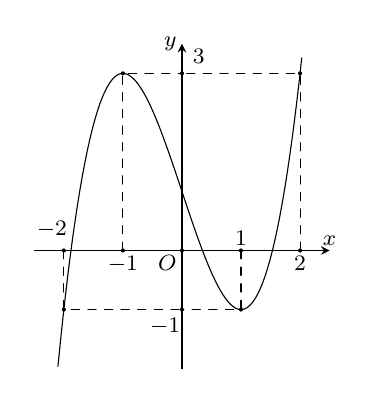
\begin{tikzpicture}[line cap=round,line join=round,font=\footnotesize,>=stealth,scale=0.75]
			\draw[->] (-2.5,0)--(2.5,0) node[above] {$x$};
			\draw[->] (0,-2)--(0,3.5) node[left] {$y$};
			\fill (0,0) circle (1pt) node [below left] {$O$}
			(-2,0) circle (1pt) node [shift={(120:2ex)}] {$-2$}
			(0,3) circle (1pt) node [shift={(45:2ex)}] {$3$}
			(0,-1) circle (1pt) node [shift={(-135:2ex)}] {$-1$}
			(1,0) circle (1pt) node [above] {$1$}
			(-1,3) circle (1pt) (1,-1) circle (1pt) (2,3) circle (1pt) (-2,-1) circle (1pt);
			\foreach \x in {-1,2} \fill (\x,0) circle (1pt) node [below] {$\x$};
			\draw [samples=100, domain=-2.1:2.03] plot (\x, {(\x)^3-3*(\x)+1});
			\draw[dashed](1,0)|-(0,-1) (-1,0)|-(0,3) (2,0)|-(0,3) (-2,0)|-(0,-1);
	\end{tikzpicture}}
	\loigiai{
		\begin{listEX}
			\item  Dựa vào đồ thị, trên $[-2;2]$, giá trị nhỏ nhất của hàm số bằng $-1$ khi $x=1$, giá trị lớn nhất của hàm số bằng $3$ khi $x=-1$.
			\item Số nghiệm của phương trình $f(x)=m$ là số điểm chung của hai đồ thị $y=f(x)$ và $y=m$.\\
			Dựa vào hình vẽ, để hai đồ thị có điểm chung trên $(-1;2)$ thì $-1\le m <3$.
			\item Từ đồ thị, ta có $f(x)>-1$, với mọi $x \in (-1;1)$. Do đó để $f(x)>a$, với mọi $x\in (-1;1)$ thì $a\le -1$.
			\item Ta có $g'(x)=(6x^2+1)\cdot f'(2x^3+x-1)$ và $$g'(x)=0\Leftrightarrow f'(2x^3+x-1)=0\Leftrightarrow \hoac{&2x^3+x-1=-1\\&2x^3+x-1=1}\Leftrightarrow\hoac{&x=0\\&x=-1\\&x=1.}$$
			Ta có $g(0)=m^2-3m-4+f(-1)=m^2-3m-1$ và $g(1)=m^2-3m-4+f(2)=m^2-3m-1$.\\
			Do $\max\limits_{x\in[0;1]}g(x)=3\Leftrightarrow m^2-3m-1=3\Leftrightarrow m^2-3m-4=0\Leftrightarrow m=-1$ hoặc $m=4$.
		\end{listEX}
	}
\end{bt}

% từ: cau-hoi/lop12/2D1_Ung_dung_dao_ham_de_khao_sat_ham_so/2D1-3-6_Toan_thuc_te_ung_dung_GTLN_GTNN_cua_ham_so.tex
\begin{ex}%[2D1V3-6]%[ma:c2b5ecba]
	 Một chất điểm chuyển động có vận tốc tức thời $v(t)$ phụ thuộc vào thời gian $t$ theo hàm số $v(t)=-t^4+24t^2+500$ (m/s). Trong khoảng thời gian từ $t=0$ (s) đến $t=10$ (s) chất điểm đạt tốc độ lớn nhất tại thời điểm nào (làm tròn kết quả đến hàng đơn vị)?
	 \choice
		 {$t=2$}
		 {\True $t=4$}
		{$t=0$} 
		 {$t=1$}
	 \loigiai{
		 Ta có $v'(t)=-4t^3+48t=-4t(t^2-12)$.\\
		Xét  phương trình $v'(t)=0\Leftrightarrow \hoac{&t=0\\&t=\pm 2\sqrt{3}.}$\\
		Bài toán  trở thành tìm giá trị lớn nhất của hàm số $v(t)$ trên đoạn $[0;10]$, ta có
		 $$v(0)=500, v(2\sqrt{3})=664, v(10)=-7100$$
		 Vậy tốc độ lớn nhất khi $t=2\sqrt{3}\approx 4$ (s).
	 }
\end{ex}

% từ: cau-hoi/lop12/2D1_Ung_dung_dao_ham_de_khao_sat_ham_so/2D1-3-6_Toan_thuc_te_ung_dung_GTLN_GTNN_cua_ham_so.tex
\begin{ex}%[2D1V3-6]%[ma:5bd32d40]
	Một chất điểm $M$ chuyển động trên một đường thẳng đi qua $O$. Để khảo sát chuyển động của $M$ người ta gắn trên đường thẳng đó một trục tọa độ  là~$Ox$ với $O$ là~điểm gốc, mỗi đơn vị trên trục tương ứng với độ dài $1$ mét. Xét trong $12$ giây đầu tiên, tọa độ $x(t)$ của $M$ tại thời điểm $t$ giây kể từ lúc bắt đầu khảo sát được cho bởi công thức $x(t)=-\dfrac{t^3}{3}+6t^2+4$.
	 \choiceTF
		{Ban  đầu $M$ ở vị trí cách $O$ một khoảng cách bằng $6$ mét}
		{\True Vận tốc tức thời của $M$ tại thời điểm  $t$ giây $(0 \leq t \leq 12)$ là~$v(t)=-t^2+12t$ (mét/giây)}
		{\True Trong suốt $6$ giây đầu tiên, vận tốc tức thời của  $M$ luôn tăng}
		{\True Xét trong $12$ giây đầu tiên, tính từ lúc bắt đầu khảo  sát đến lúc $M$ có vận tốc tức thời lớn nhất thì $M$ đi được một quãng đường dài $148$ mét}
	 \loigiai{
		\begin{itemchoice}
			\itemch Ta có $x(0)=4$ nên ban đầu, điểm $M$  cách $O$ một khoảng $4$ m.
			\itemch Vận tốc tức thời của điểm $M$ tại thời điểm $t$ giây ($0\le  t\le 12$) là
			\[v(t)=x'(t)=-t^2+12t\, (\text{m/s}).\] 
			\itemch Ta có $v'(t)=-2t+12\ge 0,\,\, \forall t\in [0; 6]$.\\ 
			Vậy trong suốt 6 giây đầu tiên,  vận tốc tức thời của $M$ luôn tăng.
			\itemch Ta có $v'(t)=-2t+12 =0\Leftrightarrow t=6$.\\ 
			Bảng biến  thiên
			\begin{center}
				\begin{tikzpicture}
					\tkzTabInit[nocadre,lgt=1.2,espcl=3.5] 
						{$t$/.6,$v'(t)$/.6,$v (t)$/2.5} 
						{$0$,$6$,$12$} 
					\tkzTabLine{,+,0,-,} 
					 \tkzTabVar{-/$0$,+/$36$,-/$0$}
				\end{tikzpicture}
			\end{center}
			Vận  tốc tức thời của điểm $M$ lớn nhất tại thời điểm $t=6$ giây.\\
			Khi  đó điểm $M$ đi được quảng đường $S=x(6)=148$ mét.
		\end{itemchoice}
	 }
\end{ex}

% từ: cau-hoi/lop12/2D1_Ung_dung_dao_ham_de_khao_sat_ham_so/2D1-3-6_Toan_thuc_te_ung_dung_GTLN_GTNN_cua_ham_so.tex
\begin{bt}%[2D1V3-6]%[ma:ca4b8d07]
	 \immini
	{Lát cắt của một vùng đất được mô hình hóa bởi hàm bậc ba $y = f(x)$ có đồ thị như hình vẽ bên (đơn vị trên các trục là km). Biết khoảng cách $OM =  2$ km; độ rộng của núi $MN = 3{,}5$ km. Độ sâu của hồ nước là $450$ m. Chiều cao của ngọn núi là bao nhiêu mét? (làm tròn đến hàng đơn vị).
	} 
	{\begin{tikzpicture}[>=stealth,line join=round,line cap=round,color=blue,font=\footnotesize,scale=1]
		\draw[->] (-2,0) -- (3,0) node[below]  {$x$(km)};
		 \draw[->] (0,-1)--(0,2.7) node[right]{$y$(km)};
		\draw (0,0)  node[below left]{$O$};
		\fill[pattern = north east lines,pattern color=cyan,smooth] (0,0) --plot[domain=0:0.6]  (\x,{-(\x)*((\x)-2)*(3*(\x)-2)})-- (0.6,0) -- cycle;
		\fill[pattern =  north west lines,pattern color=red,smooth] (0.6,0) --plot[domain=0.6:2.0] (\x,{-(\x)*((\x)-2)*(3*(\x)-2)})-- (2.0,0) -- cycle;
		\draw[violet,samples=150,smooth,domain=-0.35:2.1] plot  (\x,{-(\x)*((\x)-2)*(3*(\x)-2)});
		\draw (2,0)  node[below right]{$N$};
		 \draw (0.6,0) node[below right]{$M$};
		\draw  (-1,1.0) node[below right]{Núi};
		\draw (1.8,2.3)  node[below right]{Núi};
		\draw (0.05,-0.5) node[below  right]{\scriptsize Hồ nước};
	\end{tikzpicture}
	 }
	 \shortans{1191}
	 \loigiai{
		Hàm số bậc ba $y=f(x)$ có dạng $y = ax^3 + bx^2 + cx + d$, ($a \neq  0$).\\
		Ta có $ON = OM + MN = 2 + 3{,}5 =  5{,}5$ km.\\
		Dựa vào hình vẽ trên, ta thấy đồ thị hàm số cắt trục hoành tại các điểm  $O(0; 0)$, $M(2; 0)$ và $N(5{,}5; 0)$.\\
		Khi đó, phương trình $f(x)=0$ có ba nghiệm phân biệt  là $x = 0$; $x = 2$; $x = 5{,}5$.\\
		Suy ra $f(x) = kx(x - 2)(x - 5{,}5) = k\left(x^3 - 7{,}5x^2 + 11x\right)$ với đồ thị hàm số $\lim\limits_{x \rightarrow  +\infty} y= -\infty$ nên $k < 0$.\\
		Ta có $f'(x) = k\left(3x^2 -  15x + 11\right)$.\\
		Xét $f'(x) = 0 \Leftrightarrow k\left(3x^2 - 15x + 11\right) = 0 \Leftrightarrow 3x^2 - 15x + 11  = 0 \Leftrightarrow x = \dfrac{15 \pm \sqrt{93}}{6}$.\\
		Độ sâu của hồ  nước là $450$ m $= 0{,}45$ km nên ta có giá trị cực tiểu của đồ thị hàm số trên là $y_{CT} = -0{,}45$.\\
		Suy ra, $f\left(\dfrac{15 - \sqrt{93}}{6}\right) = -0{,}45 \Leftrightarrow k \cdot \dfrac{-135 + 31\sqrt{93}}{36} = -0{,}45 \Leftrightarrow k = \dfrac{-16{,}2}{-135  + 31\sqrt{93}}$.\\
		Chiều cao của ngọn núi tương ứng với $y_{CD} = f\left(\dfrac{15 + \sqrt{93}}{6}\right) \approx 1{,}19106 (\mathrm{km}) \approx 1\,191  (\mathrm{m})$.\\
		Vậy ngọn núi cao  khoảng $1\,191$ m.
	 }
\end{bt}

% từ: cau-hoi/lop12/2D1_Ung_dung_dao_ham_de_khao_sat_ham_so/2D1-3-6_Toan_thuc_te_ung_dung_GTLN_GTNN_cua_ham_so.tex
\begin{bt}%[2D1C3-6]%[ma:c90bf4c5]
% nguon: Archive/2024/San pham - To Latex Strong - Tex hoa Lop 12 moi - Dot 2 (Chuong 1 + 2 + 3)/San pham - To Latex Strong - Tex hoa Lop 12 moi - Dot 2 (Chuong 1 + 2 + 3)/Data/Chuong 1/Canh dieu/To 5 - Dot 16 - Chuong 1 - On tap chuong - CD - De 3.tex #884
%[Tổ 5 - Đợt 16 - Chương 1 - Ôn tập chương - CD]%[Tổng Nguyễn]
\immini{	Một vận động viên thể thao hai môn phối hợp luyện tập với một bể bơi hình chữ nhật rộng $400$ m, dài $800$ m.\\
	Vận động viên chạy phối hợp với bơi như sau: Xuất phát từ điểm $A$, chạy đến điểm $X$, và bơi từ điểm $X$ đến điểm $C$ (như hình vẽ bên). Hỏi điểm $X$ cách điểm $A$ gần bằng bao nhiêu mét để vận động viên đến $C$ nhanh nhất \textit{(kết quả làm tròn đến hàng đơn vị)}. Biết rằng vận tốc chạy là $30$ km/h, vận tốc bơi là $6$ km/h.
		\shortans{$718$}
	}{\begin{tikzpicture}[scale=0.8, font=\footnotesize,line join=round, line cap=round, >=stealth]
		\coordinate (A) at (0,3);
		\coordinate (B) at (5,3);
		\coordinate (D) at (0,0);
		\coordinate (C) at ($(B)+(D)-(A)$);
		\coordinate (X) at ($(A)!0.7!(B)$);
		\draw(A)--(B)--(C)--(D)--cycle  (X)--(C);
		\draw (0,1.5)node[ right]{$400$ m};
		\draw (2.5,0)node[ below ]{$800$ m};
		\pic[draw,thin,angle radius=2mm] {right angle = D--A--B} 
		pic[draw,thin,angle radius=2mm] {right angle = A--D--C}
		pic[draw,thin,angle radius=2mm] {right angle = D--C--B}
		pic[draw,thin,angle radius=2mm] {right angle = A--B--C};
		\foreach \i/\g in {A/90,B/90,C/-90,D/-90, X/90}{\draw[fill=black](\i) circle (1.5pt) ($(\i)+(\g:3mm)$) node[scale=1]{$\i$};}
		\end{tikzpicture}}
	\loigiai{ Đặt $BX=x$ (km), $AX=0{,}8-x$ (km). Khi đó $CX=\sqrt{0{,}16+x^2}$ (km).\\
		Điều kiện $0\leq x<0{,}8$.\\
		Tổng thời gian vận động viên chạy và bơi là \[T=\dfrac{0{,}8-x}{30}+\dfrac{\sqrt{0{,}16+x^2}}{6}=\dfrac{1}{30} \left(0{.}8-x+5\sqrt{0{,}16+x^2}\right).\]
		Đạo hàm $T'=\dfrac{1}{30}\left(-1+\dfrac{5x}{\sqrt{0{,}16}+x^2}\right)$.\\
		Ta có $T'=0\Leftrightarrow -1+\dfrac{5x}{\sqrt{0{,}16}+x^2}=0\Leftrightarrow\sqrt{0{,}16}+x^2=5x\Rightarrow 24x^2=0{,}16\Rightarrow x= \pm \dfrac{\sqrt{6}}{30}$.\\
		Thử lại ta được $x=\dfrac{\sqrt{6}}{30}$.\\
		Bảng biến thiên 
		\begin{center}
			\begin{tikzpicture}
				\tkzTabInit%[nocadre,lgt=1.2,espcl=2]
				{$x$/1,$T'$/1,$T$/2.5}{$0$,$\frac{\sqrt{6}}{30}$,$\frac{4}{5}$}  
				\tkzTabLine{,-,0,+,}
				\tkzTabVar{+/$\frac{7}{75}$,-/$T\left(\frac{\sqrt{6}}{30}\right)$,+/$\frac{\sqrt{5}}{15}$}  
			\end{tikzpicture}
		\end{center} 
		Vậy $T$ đạt giá trị nhỏ nhất bằng $T\left(\dfrac{\sqrt{6}}{30}\right)$ tại $x=\dfrac{\sqrt{6}}{30}$.\\
		 Khi đó $AX=0{,}8-\dfrac{\sqrt{6}}{30}\approx 0{,}718 \ \text{km}= 718 \ \text{m}$.
	}
\end{bt}

% từ: cau-hoi/lop12/2D1_Ung_dung_dao_ham_de_khao_sat_ham_so/2D1-5-1_Nhan_dang_do_thi.tex
\begin{ex}%[2D1N5-1]%[ma:6c9516a0]
		Cho hàm số $y=f(x)$ liên tục trên $[-3;2]$ và có bảng biến thiên như sau. Gọi $M$, $m$ lần lượt là giá trị lớn nhất và giá trị nhỏ nhất của hàm  số $y=f(x)$ trên đoạn $[-1;1]$. Tính $M+m$.
		\begin{center}
			\begin{tikzpicture}
				 \tkzTabInit[nocadre=true,lgt=1.2,espcl=2,deltacl=0.5]
					 {$x$/0.7,$f (x)$/2}
					 {$-3$,$-1$,$0$,$1$,$2$}
				 \tkzTabVar{-/$-2$,+/$3$,-/$0$,+/$2$,-/$1$}
			\end{tikzpicture}
		\end{center}
	\choice 
			{$0$} 
			{\True  $3$}
			 {$2$}
			{$1$} 
	\loigiai{Trên đoạn $[-1;1]$ ta có giá trị lớn nhất $M=3$ khi $x=-1$ và giá  trị nhỏ nhất $m=0$ khi $x=0$.\\
		 Khi đó $M=+m=3+0=3$.}
	\end{ex}

% từ: cau-hoi/lop12/2D1_Ung_dung_dao_ham_de_khao_sat_ham_so/2D1-5-1_Nhan_dang_do_thi.tex
\begin{bt}%[2D1H5-1]%[ma:ec575586]
	Khảo sát sự biến thiên và vẽ đồ thị của các hàm  số sau
	\begin{multicols}{2}
		\begin{enumerate}
			\item $y=\dfrac{x^2-x-1}{x-2}$; 
			\item  $y=\dfrac{x^2+x-2}{x+1}$;
			\item $y=\dfrac{2x^2-x+4}{x-1}$; 
			\item $y=\dfrac{x^2+2x+1}{x+3}$. 
		\end{enumerate}
	\end{multicols}
	\loigiai{ 
		\begin{enumerate}
			\item  Hàm số $y=\dfrac{x^2-x-1}{x-2}$;\\
			Tập  xác định: $D=\mathbb{R}\setminus\{2\}$.\\
			Sự biến thiên:  $y=x+1+\dfrac{1}{x-2}$.\\
			 Ta có $y'=1-\dfrac{1}{(x-2)^2}=\dfrac{x^2-4x+3}{(x-2)^2}$.\\
			 Khi đó $y'=0\Leftrightarrow \dfrac{x^2-4x+3}{(x-2)^2}=0\Leftrightarrow\hoac{&x=1\\&x=3.}$\\
			 Ta có
			\begin{itemize}
				\item $\lim\limits_{x\to-\infty}y=\lim\limits_{x\to-\infty}\dfrac{x^2-x-1}{x-2}=-\infty;  \lim\limits_{x\to+\infty}y=\lim\limits_{x\to+\infty}\dfrac{x^2-x-1}{x-2}=+\infty$.
				\item $\lim\limits_{x\to2^-}y=\lim\limits_{x\to2^-}\left(x+1+\dfrac{1}{x-2}\right)=-\infty;  \lim\limits_{x\to2^+}y=\lim\limits_{x\to2^+}\left(x+1+\dfrac{1}{x-2}\right)=+\infty$.
				\item $\lim\limits_{x\to+\infty}\left[y-(x+1)\right]=\lim\limits_{x\to+\infty}\dfrac{1}{x-2}=0; \lim\limits_{x\to-\infty}\left[y-(x+1)\right]=\lim\limits_{x\to-\infty}\dfrac{1}{x-2}=0$. 
			\end{itemize}
			Do đó, đồ thị hàm số có tiệm cận đứng là đường thẳng $x=2$, tiệm cận xiên  là đường thẳng $y=x+1$.\\
			 Bảng biến thiên
			\begin{center}
				\begin{tikzpicture}
				\tikzset{double style/.append style={double distance=1.5pt}}
				 \tkzTabInit[nocadre=false,lgt=1.2,espcl=2.5,deltacl=0.6]
					 {$x$ /0.6,$y'$ /0.6,$y$ /2}
					 {$-\infty$,$1$,$2$,$3$,$+\infty$}
				\tkzTabLine{,+,$0$,-,d,-,$0$,+,} 
				\tkzTabVar{-/$-\infty$,+/$1$,-D+/$-\infty$/$+\infty$,-/$5$,+/$+\infty$} 
			\end{tikzpicture}
			\end{center}
			Đồ  thị
			\begin{center}
				\begin{tikzpicture}[line join=round,line cap=round,>=stealth,scale=0.7]
					\tikzset{ethicknode/.style={scale=0.9}} 
					\draw[->]  (-2.6,0)--(6.1,0) node[below left] {$x$};
					\draw[->] (0,-1.6)--(0,7.1) node[below left] {$y$}; 
					\draw (0,0) node [below left] {$O$}; 
					\foreach  \x/\nx in {-2/-2,-1/,1/1,2/,3/3,4/4,5/5}
					\draw[thin] (\x,1pt)--(\x,-1pt) node [below] {$\nx$}; 
					\draw (-1,0) node  [above]{$-1$}
						 (2,0) node[below right]{$2$};
					\foreach \y/\ny in  {-1/-1,1/1,2/2,3/3,4/4,5/5,6/6}
					 \draw[thin] (1pt,\y)--(-1pt,\y) node [left] {$\ny$};
					\draw[dashed,thin](1,0)--(1,1)--(0,1); 
					\draw[dashed,thin](3,0)--(3,5)--(0,5); 
					\draw[dashed,thin]  (2,-1.5)--(2,7) node[pos=0.9,above,rotate=90]{$x=2$};
					\begin{scope}
						 \clip (-2.5,-1.5) rectangle (6,7);
						 \draw[samples=200,domain=-2.1:1.99,smooth,variable=\x] plot (\x,{(1*((\x)^2)+-1*(\x)+-1)/(1*(\x)+-2)});
						 \draw[samples=200,domain=2.01:6,smooth,variable=\x] plot (\x,{(1*((\x)^2)+-1*(\x)+-1)/(1*(\x)+-2)});
						\draw[dashed,thin] (-2.2,-1.2)--(6.1,7.1) node[pos=0.8,below,rotate=45]{$y=x+1$}; 
					\end{scope}
					\draw  (2,-2) node{\textbf{\textit{Hình 1.31}}};
				\end{tikzpicture}
			\end{center}
			\begin{itemize}
				\item Giao điểm của đồ thị hàm số với  trục tung là điểm $\left(0; \dfrac{1}{2}\right)$.
				\item Ta có $y=0 \Leftrightarrow \dfrac{x^{2}-x-1}{x-2}=0 \Leftrightarrow x=\dfrac{1-\sqrt{5}}{2}$ hoặc $x=\dfrac{1+\sqrt{5}}{2}$. Do đó giao điểm của  đồ thị hàm số với trục hoành là các điểm $\left(\dfrac{1-\sqrt{5}}{2}; 0\right)$ và $\left(\dfrac{1+\sqrt{5}}{2}; 0\right)$.
				\item Đồ thị hàm số nhận giao điểm $I(2; 3)$ của hai đường tiệm cận làm tâm đối xứng và nhận hai đường phân giác của các góc  tạo bởi hai đường tiệm cận này làm các trục đối xứng.
			\end{itemize}
			\item Hàm  số $y=\dfrac{x^2+x-2}{x+1}$;\\
			Tập xác định của hàm số: $\mathbb{R} \setminus\{-1\}$.\\ 
			Sự biến thiên: 
			\begin{itemize}
				\item Viết $y=x-\dfrac{2}{x+1}$, ta có $y^{\prime}=1+\dfrac{2}{(x+1)^{2}}>0$  với mọi $x \neq-1$.
				\item Hàm số đồng biến trên từng khoảng $(-\infty;-1)$ và $(-1;+\infty)$. 
				\item  Hàm số không có cực trị.
				 \item $\lim\limits _{x \rightarrow-\infty} y=\lim\limits _{x \rightarrow-\infty} \dfrac{x^{2}+x-2}{x+1}=\lim\limits _{x \rightarrow-\infty} \dfrac{x+1-\dfrac{2}{x}}{1+\dfrac{1}{x}}=-\infty$;\\ $\lim\limits _{x \rightarrow+\infty} y=\lim\limits _{x \rightarrow+\infty} \dfrac{x^{2}+x-2}{x+1}=\lim\limits _{x \rightarrow+\infty} \dfrac{x+1-\dfrac{2}{x}}{1+\dfrac{1}{x}}=+\infty$.
				\item Tiệm  cận:
				\begin{align*}
					&\lim\limits _{x \rightarrow-1^{-}} y=\lim\limits  _{x \rightarrow-1^{-}}\left(x-\dfrac{2}{x+1}\right)=+\infty; \lim\limits _{x \rightarrow-1^{+}} y=\lim\limits _{x \rightarrow-1^{+}}\left(x-\dfrac{2}{x+1}\right)=-\infty;\\
					&\lim\limits  _{x \rightarrow+\infty}[y-x]=\lim\limits _{x \rightarrow+\infty}\left(-\dfrac{2}{x+1}\right)=0; \lim\limits _{x \rightarrow-\infty}[y-x]=\lim\limits _{x \rightarrow-\infty}\left(-\dfrac{2}{x+1}\right)=0.
				\end{align*}
			\end{itemize}
			Do đó, đồ thị hàm số có tiệm cận  đứng là đường thẳng $x=-1$, tiệm cận xiên là đường thẳng $y=x$.\\
			 Bảng biến thiên:
			\begin{center}
				\begin{tikzpicture}[line join=round,font=\footnotesize,>=stealth,scale=1]
					 \tkzTabInit[nocadre=false,lgt=1.2,espcl=2.5,deltacl=0.6]
						 {$x$ /0.6,$y'$ /0.6,$y$ /2}
						 {$-\infty$,$-1$,$+\infty$}
					\tkzTabLine{,+,d,+,} 
					 \tkzTabVar{-/$-\infty$,+D-/$+\infty$/$-\infty$,+/$+\infty$}
				\end{tikzpicture}
			\end{center}
			Đồ thị 
			\begin{center}
				\begin{tikzpicture}[line cap=round,line join=round,font=\footnotesize,>=stealth,scale=1,x=0.5cm,y=0.5cm]
					\tikzset{label  style/.style={font=\footnotesize}}
					 \draw[->] (-6.1,0)--(6.1,0) node[below] {$x$};
					\draw[->] (0,-5.1)--(0,5.1) node[left]  {$y$};
					\draw  (0,0) node [above left] {\scriptsize$O$};
					\foreach \x/\nx  in {-6/-6,-5/-5,-4/-4,-3/-3,-2/-2,-1/,1/1,2/2,3/3,4/4,5/5}
					\draw[thin] (\x,1pt)--(\x,-1pt) node  [below] {\scriptsize$\nx$};
					\foreach \y/\ny  in {-4/right,-3/right,-2/right,-1/left,1/left,2/left,3/left,4/left}
					\draw[thin] (1pt,\y)--(-1pt,\y) node [\ny]  {\scriptsize $\y$};
					\draw[dashed,thin]  (-1,-5)--(-1,5) node[above,rotate=90,pos=0.1]{$x=-1$};
					\draw (-1,0) node[above left]{$-1$}; 
					\begin{scope}
						\clip (-6,-5) rectangle  (6,5);
						\draw[samples=200,domain=-6:-1.01,smooth,variable=\x,magenta]  plot (\x,{(1*((\x)^2)+1*(\x)+-2)/(1*(\x)+1)});
						 \draw[samples=200,domain=-0.99:6,smooth,variable=\x,magenta] plot (\x,{(1*((\x)^2)+1*(\x)+-2)/(1*(\x)+1)});
						 \draw[dashed,thin] (-6.1,-6.1)--(6.1,6.1) node[above,rotate=45,pos=0.8]{$y=x$};
					\end{scope}
					 \draw (0,-5.5) node{\textbf{\textit{Hình 1.32}}};
				\end{tikzpicture}
			\end{center}
			\begin{itemize}
				\item Giao điểm của đồ thị hàm số với  trục tung là điểm $(0;-2)$.
				\item Ta  có $y=0 \Leftrightarrow \dfrac{x^{2}+x-2}{x+1}=0 \Leftrightarrow x=-2$ hoặc $x=1$.
				Do đó giao điểm của đồ thị hàm số với trục  hoành là các điểm $(-2; 0)$ và $(1; 0)$.
				\item Đồ  thị hàm số nhận giao điểm $I(-1;-1)$ của hai đường tiệm cận làm tâm đối xứng và nhận hai đường phân giác của góc tạo bởi hai đường tiệm cận này làm các trục đối xứng.
			\end{itemize}
			\item Hàm  số $y=\dfrac{2x^2-x+4}{x-1}$;\\
			Tập xác định của hàm số: $\mathscr{D}=\mathbb{R}  \setminus\{1\}$.\\
			Sự biến thiên: 
			\begin{itemize}
				\item Viết $y=2x+1+\dfrac{5}{x-1}$, ta  có $y^{\prime}=2-\dfrac{5}{(x-1)^{2}}$ với mọi $x \neq 1$.
				Suy ra 
				\[y'=0\Leftrightarrow x=1\pm  \dfrac{\sqrt{10}}{2}. \]
				\item Trên các khoảng $\left( -\infty;1-\dfrac{\sqrt{10}}{2} \right)$  và $\left(1+\dfrac{\sqrt{10}}{2};+\infty \right)$ thì $y'>0$ nên hàm số đồng biến trên các khoảng này.\\
				Trên các khoảng $\left(1-\dfrac{\sqrt{10}}{2};1 \right)$ và $\left( 1;1+\dfrac{\sqrt{10}}{2} \right)$ thì  $y'<0$ nên hàm số nghịch biến trên các khoảng này.
				\item Đồ thị hàm số có điểm cực đại là $(x_{\text{ cđ}};y_{\text{ cđ}})=\left(1-\dfrac{\sqrt{10}}{2};3-2\sqrt{10} \right)$ và  điểm cực tiểu là $(x_{\text{ ct}},y_{\text{ ct}})=\left(1+\dfrac{\sqrt{10}}{2}; 3+2\sqrt{10} \right)$.
				\item  $\lim\limits _{x \rightarrow-\infty} y=-\infty$; $\lim\limits _{x \rightarrow+\infty} y=+\infty$.
				 \item Tiệm cận:
				\begin{align*}
					&\lim\limits _{x \rightarrow 1^{-}} y=-\infty; \lim\limits _{x \rightarrow 1^{+}} y=+\infty;\\ 
					&\lim\limits _{x \rightarrow+\infty}[y-(2x+1)]=  \lim\limits _{x \rightarrow-\infty}[y-(2x+1)]=0.
				\end{align*}
				Do đó, đồ thị hàm số có tiệm cận đứng là đường thẳng $x=1$, tiệm cận xiên là đường  thẳng $y=2x+1$.\\
				Bảng biến thiên 
				\begin{center}
					\begin{tikzpicture}[line join=round,font=\footnotesize,>=stealth,scale=1]
						 \tkzTabInit[nocadre=false,lgt=1.2,espcl=2.5,deltacl=0.6]
						{$x$ /1,$y'$ /1,$y$  /3}
						{$-\infty$,$1-\dfrac{\sqrt{10}}{2}$,$1$,$1+\dfrac{\sqrt{10}}{2}$,$+\infty$} 
						 \tkzTabLine{,+,0,-,d,-,0,+}
						\tkzTabVar{-/$-\infty$,+/$3-2\sqrt{10}$,-D+/$-\infty$/$+\infty$,-/$3+2\sqrt{10}$,+/$+\infty$} 
					\end{tikzpicture}
				\end{center}
			\end{itemize}
			Đồ thị 
			\begin{center}
				\begin{tikzpicture}[line cap=round,line join=round,font=\footnotesize,>=stealth,scale=1,x=0.5cm,y=0.25cm]
					\tikzset{label  style/.style={font=\footnotesize}}
					\draw[->] (-4,0)--(6,0) node[below] {$x$}; 
					\draw[->] (0,-8)--(0,15) node[left]  {$y$};
					\draw[smooth,samples=100,color=red] plot[domain=-4:0.5]  (\x,{(2*(\x)^2-(\x)+4)/(\x-1)});
					\draw[smooth,samples=100,color=red] plot[domain=1.5:6] (\x,{(2*(\x)^2-(\x)+4)/(\x-1)}); 
					\draw[dashed] (1,-8) node  [right]{$x=1$}--(1,15)
						plot[domain=-4:6](\x,{2*(\x)+1})  node[rotate=45,below]{$y=2x+1$}
						({1-sqrt  (10)/2},0) node[above]{$x_{\text{ cđ}}$}--({1-sqrt (10)/2},{3-2*sqrt (10)})--(0,{3-2*sqrt (10)}) node[right]{$y_{\text{ cđ}}$}
						({1+sqrt (10)/2},0) node[below]{$x_{\text{ ct}}$}--({1+sqrt  (10)/2},{3+2*sqrt (10)})--(0,{3+2*sqrt (10)}) node[left]{$y_{\text{ ct}}$};
				\end{tikzpicture}
			\end{center}
			\begin{itemize}
				\item Giao  điểm của đồ thị hàm số với trục tung là điểm $(0;-4)$.
				\item Ta có $y=0 \Leftrightarrow 2x^{2}-x+4=0$. Phương trình này vô nghiệm nên đồ thị hàm số không cắt  trục hoành.
				\item Đồ thị hàm số nhận giao điểm $I(1;3)$ của hai đường tiệm cận làm tâm đối xứng và nhận hai đường phân giác của góc tạo  bởi hai đường tiệm cận này làm các trục đối xứng.
			\end{itemize}
			 \item Hàm số $y=\dfrac{x^2+2x+1}{x+3}$;\\
			Tập  xác định của hàm số: $\mathscr{D}=\mathbb{R} \setminus\{-3\}$.\\
			 Sự biến thiên:
			\begin{itemize}
				\item Viết $y=x-1+\dfrac{4}{x+3}$, ta có $y^{\prime}=1-\dfrac{4}{(x+3)^{2}}$ với mọi  $x \neq -3$.
				Suy ra  $ y'=0\Leftrightarrow x=-5$ hoặc $x=-1$.
				\item Trên các khoảng $\left( -\infty;-5 \right)$ và $\left(-1;+\infty \right)$ thì $y'>0$  nên hàm số đồng biến trên các khoảng này.
				Trên các khoảng $\left(-5;-3 \right)$ và $\left( -3;-1\right)$ thì $y'<0$ nên hàm số nghịch biến trên các khoảng này. 
				\item Đồ thị hàm số  có điểm cực đại là $(x_{\text{ cđ}};y_{\text{ cđ}})=\left(-5;-8\right)$ và điểm cực tiểu là $(x_{\text{ ct}},y_{\text{ ct}})=\left(-1; 0 \right)$.
				\item $\lim\limits _{x \rightarrow-\infty} y=-\infty$; $\lim\limits _{x \rightarrow+\infty} y=+\infty$. 
				\item Tiệm  cận:
				\begin{align*}
					&\lim\limits _{x \rightarrow  (-3)^{-}} y=-\infty; \lim\limits _{x \rightarrow (-3)^{+}} y=+\infty;\\
					&\lim\limits  _{x \rightarrow+\infty}[y-(x-1)]= \lim\limits _{x \rightarrow-\infty}[y-(x-1)]=0.
				\end{align*}
				Do đó, đồ thị hàm số có tiệm cận đứng là đường thẳng $x=1$, tiệm cận xiên là đường thẳng $y=x-1$.\\ 
				Bảng biến  thiên
				\begin{center}
					\begin{tikzpicture}[line join=round,font=\footnotesize,>=stealth,scale=1]
						 \tkzTabInit[nocadre=false,lgt=1.2,espcl=2.5,deltacl=0.6]
						{$x$  /1,$y'$ /1,$y$ /3}
						{$-\infty$,$-5$,$-3$,$-1$,$+\infty$} 
						\tkzTabLine{,+,0,-,d,-,0,+} 
						\tkzTabVar{-/$-\infty$,+/$-8$,-D+/$-\infty$/$+\infty$,-/$0$,+/$+\infty$} 
					\end{tikzpicture}
				\end{center}
			\end{itemize}
			Đồ  thị
			\begin{center}
				\begin{tikzpicture}[line cap=round,line join=round,font=\footnotesize,>=stealth,scale=1,x=0.3cm,y=0.3cm]
					\tikzset{label  style/.style={font=\footnotesize}}
					 \draw[->] (-10,0)--(8,0) node[below] {$x$};
					\draw[->] (0,-12)--(0,7) node[left]  {$y$};
					\draw[smooth,samples=100,color=red]  plot[domain=-10:-3.5] (\x,{((\x)^2+2*(\x)+1)/(\x+3)});
					\draw[smooth,samples=100,color=red]  plot[domain=-2.6:8] (\x,{((\x)^2+2*(\x)+1)/(\x+3)});
					\draw[dashed] (-3,-12)--(-3,7) node [above left,rotate=90]{$x=-3$} 
						plot[domain=-10:8](\x,{(\x)-1})  node[rotate=45,below]{$y=x-1$}
						 (-5,0) node[above]{$x_{\text{ cđ}}$}--(-5,-8)--(0,-8) node[right]{$y_{\text{ cđ}}$};
				\end{tikzpicture}
			\end{center}
			\begin{itemize}
				\item  Giao điểm của đồ thị hàm số với trục tung là điểm $\left(0;\dfrac{1}{3}\right)$.
				\item Ta có $$y=0 \Leftrightarrow x^2+2x+1=0  \Leftrightarrow x=-1.$$
				Đồ thị hàm số cắt trục hoành  tại điểm $(0,-1)$.
				\item Đồ thị hàm số nhận giao điểm $I(-3;-4)$ của hai đường tiệm cận làm tâm đối xứng và nhận hai đường phân giác của góc tạo bởi hai đường tiệm cận  này làm các trục đối xứng.
			\end{itemize}
		\end{enumerate}
	} 
\end{bt}

% từ: cau-hoi/lop12/2D1_Ung_dung_dao_ham_de_khao_sat_ham_so/2D1-5-1_Nhan_dang_do_thi.tex
\begin{bt}%[2D1H5-1]%[ma:377ece2a]
	Khảo sát  sự biến thiên và vẽ đồ thị các hàm số sau
	\begin{multicols}{2}
		\begin{enumerate}
			\item  $y = \dfrac{x+1}{x-2}$.
			 \item $y = \dfrac{2x+1}{x+1}$.
			\item $y  = \dfrac{x+3}{1-x}$.
			\item $y =  \dfrac{5+x}{2-x}$.
		\end{enumerate}
	\end{multicols}
	\loigiai{ 
		\begin{enumerate}
			\item  Xét hàm số $y = \dfrac{x+1}{x-2}$.
			\begin{itemize}
				 \item Tập xác định $\mathscr{D}=\mathbb{R} \setminus \{2\}$.
				\item Đạo hàm $y' = \dfrac{-3}{(x-2)^2} < 0$ với mọi  $x \ne 2$. \\
				Hàm  số nghịch biến trên từng khoảng $(-\infty; 2)$ và $(2; +\infty)$ và không có cực trị.
				\item Tiệm cận 
				\begin{itemize}
					 \item Ta có $\lim\limits_{x\to 2^-}y=\lim\limits_{x\to 2^-}\dfrac{x+1}{x-2}=-\infty$; $\lim\limits_{x\to 2^+}y=\lim\limits_{x\to 2^+}\dfrac{x+1}{x-2}=+\infty
					\Rightarrow$ Tiệm cận đứng của đồ thị hàm số là  đường thẳng $x = 2$.
					\item $\lim\limits_{x\to+\infty}y=\lim\limits_{x\to+\infty}\dfrac{x+1}{x-2}=1$; $\lim\limits_{x\to-\infty}y=\lim\limits_{x\to-\infty}\dfrac{x+1}{x-2}=1\Rightarrow$ Tiệm cận ngang của đồ thị hàm số là đường thẳng $y =  1$.
				\end{itemize}
				\item Bảng  biến thiên
				\begin{center}
					\begin{tikzpicture}
						\tkzTabInit[nocadre=false,lgt=1.5,espcl=4,deltacl=0.8] 
						{$x$ /1,$f'(x)$ /1,$f (x)$  /2}
						{$-\infty$,$2$,$+\infty$} 
						 \tkzTabLine{,-,d,-,}
						\tkzTabVar{+/ $1$,-D+/$-\infty$ / $+\infty$,-/  $1$}
					\end{tikzpicture}
				\end{center}
				\item Giao điểm với trục tung $x = 0 \Rightarrow y = \dfrac{1}{-2} = -\dfrac{1}{2} \Rightarrow \left(0; -\dfrac{1}{2}\right)$. 
				\item Giao điểm với trục hoành $y = 0 \Rightarrow x +  1 = 0 \Rightarrow x = -1 \Rightarrow (-1; 0)$.
				\item Nhận xét: Đồ thị nhận điểm $I(2;1)$ là tâm đối xứng và đồ  thị nhận hai đường phân giác làm trục đối xứng.
			\end{itemize}
			\begin{center}
				\begin{tikzpicture}[scale=0.5]
					\draw[->] (-6,0)--(9,0)  node[below]{$x$};
					\draw[->]  (0,-7)--(0,7) node[left]{$y$};
					\draw[dashed] (2,-7)--(2,7) node[below left] {$x=2$}; 
					\draw[dashed] (-6,1)--(9,1) node[below left]  {$y=1$};
					\draw[domain=-6:1.62,smooth,variable=\x]  plot ({\x},{(\x+1)/(\x-2)});
					 \draw[domain=2.5:9,smooth,variable=\x] plot ({\x},{(\x+1)/(\x-2)});
					\fill (0,0) circle (1.3pt) node[above  right]{$O$};
				\end{tikzpicture}
			\end{center}
			\item  Xét hàm số $y = \dfrac{2x+1}{x+1}$.
			\begin{itemize}
				\item Tập  xác định $\mathscr{D}=\mathbb{R} \setminus \{-1\}$.
				\item Đạo hàm $y' =  \dfrac{1}{(x+1)^2} > 0$ với mọi $x \ne -1$. \\
				Hàm số đồng biến trên từng khoảng $(-\infty; -1)$ và $(-1;  +\infty)$ và không có cực trị.
				\item Tiệm cận 
				\begin{itemize}
					\item $\lim\limits_{x\to (-1)^-}y=\lim\limits_{x\to (-1)^-}\dfrac{2x+1}{x+1}=+\infty$; $\lim\limits_{x\to (-1)^+}y=\lim\limits_{x\to  (-1)^+}\dfrac{2x+1}{x+1}=-\infty
					\Rightarrow$ Tiệm cận đứng của đồ thị hàm số là đường thẳng  $x = -1$.
					\item $\lim\limits_{x\to+\infty}y=\lim\limits_{x\to+\infty}\dfrac{2x+1}{x+1}=2$; $\lim\limits_{x\to-\infty}y=\lim\limits_{x\to-\infty}\dfrac{2x+1}{x+1}=2\Rightarrow$ Tiệm cận ngang của đồ thị hàm số là  đường thẳng $y = 2$.
				\end{itemize}
				 \item Bảng biến thiên
				\begin{center}
					\begin{tikzpicture}
						\tkzTabInit[nocadre=false,lgt=1.5,espcl=4,deltacl=0.8] 
						 {$x$ /1,$f'(x)$ /1,$f (x)$ /2}
						 {$-\infty$,$-1$,$+\infty$}
						\tkzTabLine{,+,d,+,} 
						\tkzTabVar{-/ $2$,+D-/$+\infty$ / $-\infty$,+/ $2$} 
					\end{tikzpicture}
				\end{center}
				\item Giao  điểm với trục tung $x = 0 \Rightarrow y = \dfrac{1}{1} = 1 \Rightarrow (0;1)$.
				\item Giao điểm với trục hoành $y = 0 \Rightarrow 2x + 1 = 0 \Rightarrow x =  -\dfrac{1}{2} \Rightarrow \left(-\dfrac{1}{2}; 0\right)$.
				\item Nhận xét: Đồ thị nhận điểm $I(-1;2)$ là tâm đối xứng và đồ thị nhận hai đường  phân giác làm trục đối xứng.
			\end{itemize}
			\begin{center}
				\begin{tikzpicture}[scale=0.8]
					 \draw[->] (-6,0)--(4,0) node[below]{$x$};
					 \draw[->] (0,-3)--(0,6) node[left]{$y$};
					\draw[dashed] (-1,6) -- (-1,-3) node[above  left]{$x=-1$};
					\draw[dashed] (-6,2)--(4,2)  node[above left]{$y=2$};
					\draw[domain=-6:-1.26,smooth,variable=\x] plot ({\x},{(2*\x+1)/(\x+1)}); 
					\draw[domain=-0.8:4,smooth,variable=\x] plot ({\x},{(2*\x+1)/(\x+1)}); 
					\fill (0,0)  circle (1.4pt) node[below right]{$O$};
				\end{tikzpicture}
			\end{center}
			\item Xét hàm số $y  = \dfrac{x+3}{1-x}$.
			\begin{itemize}
				\item Tập xác định $\mathscr{D} = \mathbb{R} \setminus \{1\}$. 
				 \item Đạo hàm $y' = \dfrac{4}{(1-x)^2} > 0$ với mọi $x \ne 1$. \\
				Hàm số đồng biến trên các khoảng $(-\infty;1)$ và $(1;+\infty)$ và không có  cực trị.
				\item  Tiệm cận
				\begin{itemize}
					\item $\lim\limits_{x\to 1^-}y=\lim\limits_{x\to 1^-}\dfrac{x+3}{1-x}=+\infty$;  $\lim\limits_{x\to 1^+}y=\lim\limits_{x\to 1^+}\dfrac{x+3}{1-x}=-\infty
					\Rightarrow$  Tiệm cận đứng của đồ thị hàm số là đường thẳng $x = 1$.
					\item $\lim\limits_{x\to+\infty}y=\lim\limits_{x\to+\infty}\dfrac{x+3}{1-x}=-1$; $\lim\limits_{x\to-\infty}y=\lim\limits_{x\to-\infty}\dfrac{x+3}{1-x}=-1\Rightarrow$ Tiệm cận ngang của đồ thị hàm số là  đường thẳng $y = -1$.
				\end{itemize}
				\item Bảng biến thiên 
				\begin{center}
					\begin{tikzpicture}
						\tkzTabInit[nocadre=false,lgt=1.5,espcl=4,deltacl=0.8] 
						{$x$ /1,$f'(x)$ /1,$f  (x)$ /2}
						{$-\infty$,$1$,$+\infty$} 
						 \tkzTabLine{,+,d,+,}
						\tkzTabVar{-/ $-1$,+D-/$+\infty$ / $-\infty$,+/ $-1$} 
					\end{tikzpicture}
				\end{center}
				\item Giao điểm với trục tung $(0;3)$, giao điểm với  trục hoành $(-3;0)$.
				\item Đồ thị  nhận giao điểm $I(1;-1)$ làm tâm đối xứng.
			\end{itemize}
			\begin{center}
				\begin{tikzpicture}[scale=0.5]
					\draw[->] (-7,0)--(9,0)  node[below]{$x$};
					\draw[->] (0,-7)--(0,7)  node[left]{$y$};
					\draw[dashed] (1,-7)--(1,7) node[below  right]{$x=1$};
					\draw[dashed] (9,-1)--(-7,-1) node[below right]{$y=-1$}; 
					\draw[domain=-7:0.5,smooth,variable=\x] plot  ({\x},{(\x+3)/(1-\x)});
					\draw[domain=1.7:9,smooth,variable=\x] plot ({\x},{(\x+3)/(1-\x)}); 
					\fill (0,0)  circle (1.4pt) node[above right]{$O$};
				\end{tikzpicture}
			\end{center}
			\item Xét  hàm số $y = \dfrac{5+x}{2-x}$.
			\begin{itemize}
				\item Tập xác định $\mathscr{D}=\mathbb{R}  \setminus \{2\}$.
				\item Đạo hàm $y' = \dfrac{7}{(-x+2)^2} > 0$  với mọi $x \ne 2$. \\ Hàm số đồng biến trên các khoảng $(-\infty;2)$ và $(2;+\infty)$.
				 \item Tiệm cận
				\begin{itemize}
					\item $\lim\limits_{x\to 2^-}y=\lim\limits_{x\to 2^-}\dfrac{5+x}{2-x}=+\infty$; $\lim\limits_{x\to 2^+}y=\lim\limits_{x\to 2^+}\dfrac{5+x}{2-x}=-\infty 
					\Rightarrow$ Tiệm cận đứng của đồ thị hàm số  là đường thẳng $x = 2$.
					\item $\lim\limits_{x\to+\infty}y=\lim\limits_{x\to+\infty}\dfrac{5+x}{2-x}=-1$; $\lim\limits_{x\to-\infty}y=\lim\limits_{x\to-\infty}\dfrac{5+x}{2-x}=-1\Rightarrow$ Tiệm cận ngang của đồ thị hàm số là  đường thẳng $y = -1$.
				\end{itemize}
				 \item Bảng biến thiên
				\begin{center}
					\begin{tikzpicture}
						 \tkzTabInit[nocadre=false,lgt=1.5,espcl=4,deltacl=0.8]
						{$x$  /1,$f'(x)$ /1,$f (x)$ /2}
						 {$-\infty$,$2$,$+\infty$}
						 \tkzTabLine{,+,d,+,}
						\tkzTabVar{-/ $-1$,+D-/$+\infty$ /  $-\infty$,+/ $-1$}
					\end{tikzpicture}
				\end{center}
				\item Giao  điểm với trục tung $(0;3)$, giao điểm với trục hoành $(-5;0)$.
				\item Đồ thị nhận  điểm $I(2;-1)$ là tâm đối xứng.
			\end{itemize}
			\begin{center}
				\begin{tikzpicture}[scale=0.4]
					 \draw[->] (-8,0)--(11,0) node[below]{$x$};
					\draw[->] (0,-8)--(0,8) node[left]{$y$}; 
					\draw[dashed] (2,-8)--(2,8) node[below right]{$x=2$}; 
					\draw[dashed] (11,-1)--(-8,-1)  node[below right]{$y=-1$};
					\draw[domain=-8:1.25,smooth,variable=\x] plot  ({\x},{(5+\x)/(2-\x)});
					\draw[domain=2.95:11,smooth,variable=\x] plot  ({\x},{(5+\x)/(2-\x)});
					\fill (0,0) circle (1.4pt) node[above right]{$O$}; 
				\end{tikzpicture}
			\end{center}
		\end{enumerate}
	} 
\end{bt}

% từ: cau-hoi/lop12/2D1_Ung_dung_dao_ham_de_khao_sat_ham_so/2D1-5-3_Bien_luan_so_giao_diem_dua_vao_do_thi_bang_bi.tex
\begin{bt}%[2D1N5-3]%[ma:13152e2d]
% nguon: Archive/2024/TaiLieuGiangDay/1.HamSo/1. K12 - 4in1 - Hamso/ThubaiGoc/Bai5-Dang6.tex #2211

	Cho hàm số $f(x)$ có bảng biến thiên như sau
	\begin{center}
		\begin{tikzpicture}[>=stealth,scale=1]
			\tkzTabInit[lgt=1.2,espcl=3]
			{$x$ /1.2, $f’(x)$ /1.2, $f(x)$ /2.5}
			{$-\infty$,$-1$,$1$,$+\infty$}
			\tkzTabLine{ ,+,0,-,0,+, }
			\tkzTabVar{-/$-\infty$,+/$4$,-/$0$,+/$+\infty$}
		\end{tikzpicture}
	\end{center}
	Xác định số nghiệm của phương trình $f(x) + 7 = 0$.
	\loigiai{
		Ta nhận thấy hàm số nhận giá trị $-7$ tại đúng một điểm trong mỗi khoảng $(-\infty;-1)$ và $(1;+\infty )$ nhưng không nhận giá trị $-7$ trong $(-1;1)$. Do đó, phương trình $f(x) + 7 = 0$ có $2$ nghiệm.
	}
\end{bt}

% từ: cau-hoi/lop12/2D1_Ung_dung_dao_ham_de_khao_sat_ham_so/2D1-5-7_Diem_dac_biet_cua_do_thi_ham_so.tex
\begin{ex}%[2D1H5-7]%[ma:5759121d]
	Cho hàm số $y=-\dfrac{-x^2-3x+4}{x-3}$ có đồ thị  là $(C)$.
	\choiceTF 
		 {\True Đồ thị $(C)$ có tiệm cận xiên là $y=-x-6$}
		{\True Đồ thị $(C)$ nhận điểm $I(3; -9)$ làm tâm đối  xứng}
		{\True Đồ thị $(C)$ có hai điểm cực trị nằm  2 phía đối với trục $Oy$}
		{Đồ thị không cắt trục $Ox$} 
	 \loigiai{
		\begin{itemchoice}
			\itemch Tập xác định $\mathscr{D}=\mathbb{R}\setminus\{3\}$.\\ 
			Ta có $y=\dfrac{-x^2-3x+4}{x-3}=-x-6-\dfrac{14}{x-3}$.\\ 
			 Khi đó $\lim\limits_{x \rightarrow+\infty}[f(x)-(-x-6)]=\lim\limits_{x \rightarrow+\infty}\left(-\dfrac{14}{x-3}\right)=0$.\\
			Khi đó đường thẳng  $y=-x-6$ là đường tiệm cận xiên của đồ thị hàm số.
			\itemch Lại có  $\lim\limits_{x\to3^+}f(x)=\lim\limits_{x\to3^+}\dfrac{-x^2-3x+4}{x-3}=-\infty$.\\
			Do đó đồ  thị hàm số nhận đường thẳng $x=3$ là đường tiệm cận đứng.\\
			Suy ra tâm đối xứng là  $I(3;-9)$
			 \itemch Ta có $y'=\dfrac{-x^2+6x+5}{(x-3)^2}=0\Leftrightarrow x^2-6x-5=0\Leftrightarrow\hoac{&x=3+\sqrt{14}\\&x=3-\sqrt{14}.}$\\
			Do đó đồ thị hàm số có hai điểm cực trị nằm  về hai phía của trục tung.\\
			Ta có $y=0\Leftrightarrow  -x^2-3x+4=0\Leftrightarrow\hoac{&x=1\\&x=-4}$.\\
			\itemch Do đó đồ thị hàm số cắt trục $Ox$ tại  hai điểm phân biệt.
		\end{itemchoice}
	} 
\end{ex}

% từ: cau-hoi/lop12/2D1_Ung_dung_dao_ham_de_khao_sat_ham_so/2D1-5-8_Toan_thuc_te_ung_dung_khao_sat_ham_so.tex
\begin{bt}%[2D1V5-8]%[ma:51b8505f]
	\immini{Công ty Viễn thông Viettel dựng hai cột ăng-ten thẳng đứng cao $10$ m và $30$ m lần lượt tại hai vị trí $A$, $B$ cách nhau một khoảng bằng $24$ m Người ta chọn một chốt tại vị trí $M$ trên mặt đất nằm giữa hai chân cột để giăng dây néo đến hai đỉnh $C$ và $D$ của ăng-ten (xem hình vẽ minh họa). Hỏi phải đặt chốt $M$ ở vị trí cách điểm $A$ bao~nhiêu mét trên mặt đất để tổng độ dài của hai đoạn dây néo là ngắn nhất?}{\begin{tikzpicture}[line join=round,line cap=round,>=stealth,font=\scriptsize]
		\path (0:0) coordinate (A) 
			(90:1.5) coordinate (C) 
			(0:1) coordinate  (M)
			(0:4)  coordinate (B)
			($(B)+(90:4.5)$) coordinate  (D);
		 \draw (A)--(M)--(C)--cycle
			(B)--(M)--(D)--cycle; 
		\foreach \t/\g in  {A/-90,M/-90,C/90,B/-90,M/-90,D/90}{
			\fill  (\t) circle (1pt) node[shift={(\g:9pt)}]{$ \t $};
		} 
		\path  (A)--(C) node[midway,left]{$10$ m}
			(B)--(D) node[midway,right]{$30$ m}; 
		\foreach \x/\y/\z in {D/B/M,M/A/C}{ 
			\path pic[draw,angle  radius=5pt]{right angle= \x--\y--\z};
		 }
	\end{tikzpicture}
	} 
	\shortans{6} 
	 \loigiai{
		\begin{itemize}
			\item Đặt $AM=x\Rightarrow x\in  ( 0;24)$, suy ra $BM=24-x$.
			\item Tổng độ dài sợi dây néo cần dùng là  $L=CM+MD=\sqrt {10^2+x^2}+\sqrt {30^2+( 24-x)^2}$.
			\item  Xét hàm số $ y=\sqrt {10^2+x^2}+\sqrt {30^2+( 24-x)^2}$, $(0<x<24)$.\\
			$y'=\dfrac {x}{\sqrt {10^2+x^2}}+\dfrac  {-24+x}{\sqrt {30^2+( 24-x)^2}}$, $(0<x<24)$.\\
			$y'=0\Leftrightarrow x=6$.\\ 
			Bảng biến thiên 
			\begin{center}
				\begin{tikzpicture}
					\tkzTabInit[nocadre,espcl=3.5,lgt=2.5,deltacl=1.5] 
						{$x$/0.7,$y'$/0.7,$y$/2.5} 
						{$0$,$6$,$24$} 
					 \tkzTabLine{,-,0,+,}
					 \tkzTabVar{+/$10+6\sqrt{41}$,-/$8\sqrt{34}$,+/$56$}
				\end{tikzpicture}
			\end{center}
			Suy ra  $AM=x=6$.\\
			Vậy phải đặt chốt $M$ ở vị trí cách $A$ bằng $6$ m trên mặt đất nằm giữa $A$ và $B$ thì tổng độ dài của hai đoạn dây  néo là ngắn nhất.
		\end{itemize}
	 }
\end{bt}

% từ: cau-hoi/lop12/2D3_Cac_so_dac_trung_ghep_nhom/2D3-1-2_Tim_khoang_bien_thien.tex
\begin{ex}%[2D3H1-2]%[ma:99cdb1bf]
	Một công ty giống cây trồng đã thử nghiệm hai phương pháp chăm sóc khác nhau cho cây  hướng dương. Sau hai tuần, người ta thấy cây được chăm sóc theo cả hai phương pháp đều thấp hơn 50 cm.
	\begin{center}
		\begin{tabular}{cc}
			\begin{tikzpicture}[scale=1,>=stealth,font=\footnotesize,line join=round,line cap=round,x=1mm,y=2mm]
					 \def\xmin{0} \def\xmax{60} \def\ymin{0} \def\ymax{15}
					\draw[color=gray!50,help lines,xstep=2mm,ystep=2mm] (\xmin,\ymin)  grid (\xmax,\ymax);
					\draw[->] (\xmin,0)--(\xmax,0) node [below]{cm}; 
					\draw[->] (0,\ymin)--(0,\ymax) node [above]{Tần  số};
					\node at (0,0)  [xshift=-2mm,yshift=-2mm]{$O$};
					\foreach \x in  {10,20,30,40,50}
					\draw (\x,1pt)--(\x,-2pt) node  [below] {$\x$};
					 \foreach \y in {5,10}
					\draw (1pt,\y)--(-2pt,\y) node [left]  {$\y$};
					\fill[blue,opacity=.75]  (0,0)--(0,6)--(10,6)--(10,8)--(20,8)--(20,12)--(30,12)--(30,8)--(40,8)--(40,6)--(50,6)--(50,0);
				\end{tikzpicture}
			 &
			\begin{tikzpicture}[scale=1,>=stealth,font=\footnotesize,line join=round,line cap=round,x=1mm,y=2mm]
					 \def\xmin{0} \def\xmax{60} \def\ymin{0} \def\ymax{15}
					 \draw[color=gray!50,help lines,xstep=2mm,ystep=2mm] (\xmin,\ymin) grid (\xmax,\ymax);
					\draw[->]  (\xmin,0)--(\xmax,0) node [below]{cm};
					 \draw[->] (0,\ymin)--(0,\ymax) node [above]{Tần số};
					 \node at (0,0) [xshift=-2mm,yshift=-2mm]{$O$};
					 \foreach \x in {10,20,30,40,50}
					\draw (\x,1pt)--(\x,-2pt)  node [below] {$\x$};
					\foreach  \y in {5,10}
					\draw (1pt,\y)--(-2pt,\y) node  [left] {$\y$};
					\fill[blue,opacity=.75] (0,0)--(0,13)--(10,13)--(10,6)--(20,6)--(20,2)--(30,2)--(30,6)--(40,6)--(40,13)--(50,13)--(50,0); 
				\end{tikzpicture}
			\\ 
			\begin{tabular}{c}
				Chiều cao của cây chăm sóc\\ theo phương án  A
			\end{tabular}
			 &
			\begin{tabular}{c}
				Chiều cao của cây chăm sóc\\ theo phương  án B
			\end{tabular}
		\end{tabular}
	\end{center}
	 \choiceTF
		{\True Khoảng  biến thiên của chiều cao các cây được chăm sóc theo mỗi phương pháp $A$ và $B$ bằng nhau}
		{\True Trung bình của chiều cao các cây được chăm sóc theo  mỗi phương pháp $A$ và $B$ bằng nhau}
		{Độ lệch chuẩn của  chiều cao các cây được chăm sóc theo phương án $A$ là $12{,}65$(cm)}
		{Dựa vào độ lệch chuẩn thì chiều cao của các loại cây được chăm sóc theo phương án $B$ ít bị  chênh lệch hơn so với phương án $A$}
	\loigiai{ 
		\begin{itemchoice}
			\itemch Đúng: Khoảng biến thiên của chiều cao các  cây được chăm sóc theo mỗi phương pháp $A$ và $B$ bằng nhau và cùng bằng 50.
			\itemch Đúng: Ước tính số trung bình và độ lệch chuẩn của chiều cao các cây được chăm sóc theo mỗi phương pháp. Cỡ mẫu của hai mẫu số liệu thống kê là $N=40$. Ta có bảng tần số ghép nhóm về chiều  cao của cây được chăm sóc theo phương pháp $A$ như sau: \\
			\centerline{ 
			\begin{tabular}{|*{6}{c|}}\hline
				Chiều cao (cm)& $[0;10)$& $[10;20)$& $[20;30)$& $[30;40)$&  $[40;50)$\\\hline
				Giá trị đại diện& $5$& $15$& $25$&  $35$& $45$\\
				Tần  số& $6$& $8$& $12$& $8$& $6$\\\hline
			\end{tabular}
			}\\ 
			Chiều cao trung bình của các cây được chăm  sóc theo phương án $A$ là:\\
			$\overline{x}_A=\dfrac{5\cdot 6+18\cdot  5+25\cdot 12+35\cdot 8+45\cdot 6}{40}=25$.\\
			Ta có bảng tần số ghép nhóm về chiều cao của cây được chăm sóc theo  phương pháp $B$ như sau: \\
			\centerline{ 
			\begin{tabular}{|*{6}{c|}}\hline
				Chiều cao  (cm)& $[0;10)$& $[10;20)$& $[20;30)$& $[30;40)$& $[40;50)$\\\hline
				Giá  trị đại diện& $5$& $15$& $25$& $35$& $45$\\
				Tần  số& $13$& $6$& $2$& $6$& $13$\\\hline
			\end{tabular}
			 }\\
			Chiều cao  trung bình của các cây được chăm sóc theo phương án $B$ là: \\
			 $\overline{x}_B=\dfrac{5\cdot 13+15\cdot 6+25\cdot 2+35\cdot 6+45\cdot 13}{40}=25$ cm.
			\itemch Độ lệch  chuẩn của chiều cao các cây được chăm sóc theo phương án $A$ là:\\
			$s_A=\sqrt{\dfrac{5^2\cdot 6+15^2\cdot 8+25^2\cdot 12+35^2\cdot  8+45^2\cdot 6}{40}-25^2}\approx 12{,}65$.
			\itemch Độ lệch chuẩn của chiều cao các cây được  chăm sóc theo phương án $B$ là:\\
			$s_B=\sqrt{\dfrac{5^2\cdot 13+15^2\cdot 6+25^2\cdot  2+35^2\cdot 6+45^2\cdot 13}{40}-25^2} \approx 17{,}03$ $\rm cm^2$.
		\end{itemchoice}
	} 
\end{ex}

% từ: cau-hoi/lop12/2D4_Nguyen_ham_tich_phan/2D4-1-2_Nguyen_ham_co_ban_da_thuc_phan_thuc.tex
\begin{ex}%[2D4N1-2]%[ma:334b5858]
	Khẳng định  nào đúng?
	 \choice
		{\True  $\displaystyle\int\left(x-\dfrac{1}{x}\right)^2\mathrm{\,d}x=\dfrac{x^3}{3}-2x-\dfrac{1}{x}+C$}
		{$\displaystyle\int\left(x-\dfrac{1}{x}\right)^2\mathrm{\,d}x=\dfrac{x^3}{3}-2x+\dfrac{1}{x}+C$} 
		{$\displaystyle\int\left(x-\dfrac{1}{x}\right)^2\mathrm{\,d}x=\dfrac{1}{3}\left(x-\dfrac{1}{x}\right)^3+C$} 
		 {$\displaystyle\int\left(x-\dfrac{1}{x}\right)^2\mathrm{\,d}x=\dfrac{1}{3}\left(x-\dfrac{1}{x}\right)^3\left(1+\dfrac{1}{x^2}\right)+C$}
	 \loigiai{
		Ta  có $\displaystyle\int\left(x-\dfrac{1}{x}\right)^2\mathrm{\,d}x=\displaystyle\int\left(x^2-2+\dfrac{1}{x^2}\right)\mathrm{\,d}x=\dfrac{x^3}{3}+2x-\dfrac{1}{x}+C$
	 }
\end{ex}

% từ: cau-hoi/lop12/2D4_Nguyen_ham_tich_phan/2D4-1-2_Nguyen_ham_co_ban_da_thuc_phan_thuc.tex
\begin{ex}%[2D4H1-2]%[ma:64587173]
	Cho hàm số $F(x)=\displaystyle\int \left(\sqrt[5]{x^3}\right)\mathrm{\,d}x$  (với $x>0$). Khi đó
	 \choiceTF
		{$F(x)=\dfrac{3}{5}\displaystyle\int x\mathrm{\,d}x$} 
		{\True $F(x)+C=\displaystyle\int \left(\sqrt[5]{x^3}\right)\mathrm{\,d}x$, $C\in \mathbb{R}$} 
		 {$F(x)=\dfrac{3}{5}x^{-\tfrac{2}{5}}+C$}
		{Biết $F(1)=-\dfrac{3}{8}$, khi đó $F(x)=\dfrac{5}{8}\sqrt[5]{x^8}-\dfrac{3}{8}$} 
	 \loigiai{
		\begin{itemchoice}
			\itemch Ta có $F(x)=\displaystyle\int \left(\sqrt[5]{x^3}\right)\mathrm{\,d}x =  \displaystyle\int x^{\tfrac{3}{5}}\mathrm{\,d}x$.
			\itemch Nếu $F(x),G(x)$ là nguyên hàm của hàm  số $f(x)$ thì $F(x)=G(x)+C$.
			\itemch Ta có $F(x)=\displaystyle\int x^{\tfrac{3}{5}}\mathrm{\,d}x  = \dfrac{5}{8}x^{\tfrac{8}{5}}+C$.
			\itemch Ta có $F(x)=\dfrac{5}{8}x^{\tfrac{8}{5}}+C$, $F(1)=\dfrac{5}{8}+C=-\dfrac{3}{8} \Rightarrow C=-1  \Rightarrow F(x)=\dfrac{5}{8}\sqrt[5]{x^8}-1$.
		\end{itemchoice}
	} 
\end{ex}

% từ: cau-hoi/lop12/2D4_Nguyen_ham_tich_phan/2D4-1-2_Nguyen_ham_co_ban_da_thuc_phan_thuc.tex
\begin{bt}%[2D4H1-2]%[ma:ed43b920]
	Cho hàm số $f(x)$ có đạo hàm $f'(x)=\dfrac{3x^3+1}{x}$. Khi  đó hãy tính giá trị biểu thức $f(-3)+f(3)$ biết $f(1)=2$, $f(-1)=3$.
	\loigiai{ 
		\begin{eqnarray*}
			f(x)  &= &\displaystyle\int f'(x)\mathrm{\,d}x=\displaystyle\int \dfrac{3x^3+1}{x} \mathrm{d} x\\
			&=& \displaystyle\int\left(3x^2+\dfrac{1}{x}\right)\mathrm{\,d}x=x^3+\ln|x|+C=\heva{&x^3+\ln x+C_1\text{ khi } x > 0\\ 
			&x^3+\ln(-x)+C_2\text{ khi } x <  0}
		\end{eqnarray*}
		 $f(1)=1+C_1=2\Rightarrow C_1=1; f(-1)=-1+C_2=3\Rightarrow C_2=4$.\\
		Suy ra $f(x)=\heva{&x^3+\ln x+1\,\text{ khi  } x > 0\\
		&x^3+\ln(-x)+4\,\text{ khi } x  < 0}$ nên $f(-3)+f(3)=2\ln 3+5$.
	} 
\end{bt}

% từ: cau-hoi/lop12/2D4_Nguyen_ham_tich_phan/2D4-1-3_Nguyen_ham_co_ban_ham_luong_giac.tex
\begin{bt}%[2D4V1-3]%[ma:040475c8]
	Một vật chuyển động với vận tốc là $v(t)=\dfrac{1}{2\pi}+\dfrac{\sin (\pi t)}{\pi}\, (\mathrm{m}/\mathrm{s})$. Gọi $S_1$ là quãng đường vật đó đi trong $2$ giây đầu và $S_2$ là quãng  đường đi từ giây thứ $3$ đến giây thứ $5$. Chứng minh $S_2>S_1$?
	\loigiai{ 
		Gọi  thời điểm ban đầu $S(0)=0;t=0;S=0\Rightarrow S_1=S(2)$. \\
		Khi  đó
		\[\displaystyle S(t)=\int \left[\dfrac{1}{2\pi}+\dfrac{\sin (\pi  t)}{\pi}\right]\mathrm{\,d}t
		 =\dfrac{1}{2\pi}t-\dfrac{1}{\pi^2}\cos (\pi t)+C.\]
		Ta có $S(0)=0\Rightarrow C-\dfrac{1}{\pi^2}=0\Rightarrow  C=\dfrac{1}{\pi^2}$. \\
		Suy ra  $S(t)=\dfrac{1}{2\pi}-\dfrac{1}{\pi^2}\cos (\pi t)+\dfrac{1}{\pi^2}$. \\
		 $S_1=S(2)=\dfrac{1}{2\pi}-\dfrac{1}{\pi^2}+\dfrac{1}{\pi^2}
		=\dfrac{1}{2\pi}\approx 0{,}159$;  \\
		$\displaystyle S_2=\int_3^5 v(t)\mathrm{\,d}t\approx  0{,}31
		\Rightarrow  S_2>S_1$ (đpcm).
	 }
\end{bt}

% từ: cau-hoi/lop12/2D4_Nguyen_ham_tich_phan/2D4-1-4_Nguyen_ham_co_ban_ham_mu_luy_thua.tex
\begin{ex}%[2D4H1-4]%[ma:84aa2e85]
	Cho  hàm số $F(x)=\displaystyle\int\left(4^x+2^x+1\right)\mathrm{\,d}x$.
	\choiceTF 
		{\True  $F(x)=\displaystyle\int 4^x\mathrm{\,d}x+\displaystyle\int 2^x\mathrm{\,d}x+\displaystyle\int\mathrm{\,d}x$}
		{$F(x)=\dfrac{2^{2x}+2^x}{\ln  2}+x+C$}
		{Nếu $F(1)=\dfrac{4}{\ln 2}$ thì  $F(2)=\dfrac{12}{\ln 2}-1$}
		{Nếu $G(x)=\displaystyle\int \dfrac{8^x+1}{2^x+1}\mathrm{\,d}x$ thì  $G(x)=F(x)+C$}
	 \loigiai{
		\begin{itemchoice}
			\itemch Ta có \[F(x)=\displaystyle\int\left(4^x+2^x+1\right)\mathrm{\,d}x=\displaystyle\int 4^x\mathrm{\,d}x+\displaystyle\int 2^x\mathrm{\,d}x+\displaystyle\int\mathrm{\,d}x.\] 
			\itemch Ta có \[F(x)=\displaystyle\int\left(4^x+2^x+1\right)\mathrm{\,d}x=\dfrac{4^x}{\ln 4}+\dfrac{2^x}{\ln 2}+x+C=\dfrac{2^{2x}}{2\ln 2}+\dfrac{2^x}{\ln  2}+x+C=\dfrac{2^{2x-1}+2^x}{\ln 2}+x+C.\]
			\itemch Thay $x=1$  vào $F(x)$ ta được
			 \[F(1)=\dfrac{2^{1}+2^1}{\ln 2}+1+C=\dfrac{4}{\ln 2}+1+C=\dfrac{4}{\ln 2} \Rightarrow C=-1.\]
			 Suy ra $F(x)=\dfrac{2^{2x-1}+2^x}{\ln 2}+x-1$.\\
			 Suy ra $F(2)=\dfrac{2^{3}+2^2}{\ln 2}+2-1=\dfrac{12}{\ln 2}+1$.
			\itemch Ta có \[G(x)=\dfrac{8^x+1}{2^x+1}=\dfrac{2^{3x}+1}{2^x+1}=\dfrac{(2^x+1)(4^x-2^x+1)}{2^x+1}=4^x-2^x+1.\] 
		\end{itemchoice}
	} 
\end{ex}

% từ: cau-hoi/lop12/2D4_Nguyen_ham_tich_phan/2D4-2-6_Toan_thuc_te_ap_dung_nguyen_ham.tex
\begin{ex}%[2D4H2-6]%[ma:2631916b]
	Một chất điểm $A$ xuất phát từ $O$, chuyển động thẳng với vận tốc biến thiên theo thời gian bởi quy luật $v(t)=\dfrac{1}{150}t^2+\dfrac{59}{75}t$ (m/s), trong đó $t$ (giây) là khoảng thời gian tính từ lúc $A$ bắt đầu chuyển động. Tại trạng thái nghỉ, một chất điểm $B$ cũng xuất phát  từ $O$, chuyển động thẳng cùng hướng với $A$ nhưng chậm hơn $3$ giây so với $A$ và có gia tốc bằng $a$ (m/s$^2$) ($a$ là hằng số). Sau khi $B$ xuất phát được $12$ giây thì đuổi kịp $A$. Vận tốc của $B$ tại thời điểm đuổi kịp $A$ bằng
	 \choice
		{$15$ (m/s)} 
		{$20$ (m/s)} 
		{\True $16$ (m/s)} 
		{$13$ (m/s)} 
	 \loigiai{
		Quãng đường chất điểm $A$ đi từ đầu đến  khi $B$ đuổi kịp là $S=\displaystyle\int_{0}^{15}{\left(\dfrac{1}{150}t^2+\dfrac{59}{75}t\right)\mathrm{\,d}t}=96$ (m).\\
		Vận  tốc của chất điểm $B$ là $v_B(t)=\displaystyle\int a\mathrm{\,d}t=at+C$.\\
		Tại thời điểm $t=3$  vật $B$ bắt đầu từ trạng thái nghỉ nên $v_B(3)=0 \Leftrightarrow C=-3a$.\\
		Mặt khác quãng đường chất điểm  $B$ đi được đến khi gặp $A$ là\\
		$S_2=\displaystyle\int_{3}^{15}{\left(at-3a\right)\mathrm{\,d}t}=\left(\dfrac{at^2}{2}-3at\right)\bigg|_{3}^{15}=72a$  (m).\\
		 Vậy $72a=96 \Leftrightarrow a=\dfrac{4}{3}$ (m/s$^2$).\\
		Tại thời điểm đuổi kịp $A$ thì vận tốc  của $B$ là $v_B(15)=16$ (m/s).
	} 
\end{ex}

% từ: cau-hoi/lop12/2D4_Nguyen_ham_tich_phan/2D4-2-6_Toan_thuc_te_ap_dung_nguyen_ham.tex
\begin{ex}%[2D4H2-6]%[ma:05186c5b]
	Một chất điểm $A$ xuất phát từ $O$, chuyển động thẳng với vận tốc biến thiên theo thời gian bởi quy luật $v(t) = \dfrac{1}{120}t^2 + \dfrac{58}{45}t$ (m/s), trong đó $t$ (giây) là khoảng thời gian tính từ lúc $A$ bắt đầu chuyển động. Từ trạng thái nghỉ, một chất điểm $B$ cũng xuất phát từ $O$, chuyển động thẳng cùng hướng với $A$ nhưng chậm hơn $3$ giây so với $A$ và có gia tốc bằng $a$ (m/s$^2$) ($a$ là hằng số). Sau khi $B$ xuất phát được $15$ giây  thì đuổi kịp $A$. Vận tốc của $B$ tại thời điểm đuổi kịp $A$ bằng
	\choice 
		{$21$ (m/s)} 
		 {$25$ (m/s)}
		 {$36$ (m/s)}
		{\True $30$ (m/s)} 
	 \loigiai{
		Thời điểm chất điểm $B$ đuổi kịp chất điểm $A$ thì chất điểm $B$ đi được $15$ giây, chất điểm $A$  đi được $18$ giây.\\
		Biểu thức vận tốc của chất điểm $B$ có dạng $v_B(t) = \displaystyle\int a\mathrm{\,d}t =  at + C$ mà $v_B(0)=0$ nên $v_B(t) = at$.\\
		Do từ lúc chất điểm $A$ bắt đầu chuyển động cho đến khi chất điểm $B$ đuổi kịp thì quãng đường hai chất điểm đi được  bằng nhau.\\
		Do đó $\displaystyle\int_{0}^{18}\left(\dfrac{1}{120}t^2  + \dfrac{58}{45}t\right)\mathrm{\,d}t = \displaystyle\int_{0}^{15} at\mathrm{\,d}t \Leftrightarrow 225 = a\cdot \dfrac{225}{2} \Leftrightarrow a=2$.\\
		Vậy vận tốc của chất điểm $B$ tại thời điểm đuổi kịp $A$ bằng $v_B(t)=2\cdot 15=30$ (m/s). 
	 }
\end{ex}

% từ: cau-hoi/lop12/2D4_Nguyen_ham_tich_phan/2D4-2-6_Toan_thuc_te_ap_dung_nguyen_ham.tex
\begin{bt}%[2D4V2-6]%[ma:142fdb40]
	Một vật chuyển động với  vận tốc được cho bởi đồ thị ở hình vẽ dưới đây:
	\begin{center}
		\begin{tikzpicture}
				 \def\xmax{2.7}
				 \def\ymax{2.7}
				\draw[->] (0,-.5)  -- (0,\ymax) node[above left]{$v\,\text{ (km/phút)}$};
				\draw[->] (-.5,0) -- (\xmax,0) node[above right] {$t\,\text{  (s)}$};
				\node at (0,0) [below left]  {$O$};
				\draw  (0,0)--(1,2)--(2,2);
				\draw[dashed] (0,2)  node[left]{$2$}--(1,2)--(1,0) node[below]{$1$}
					 (2,2)--(2,0) node[below]{$2$};
			\end{tikzpicture}
	\end{center}
	\begin{enumerate}
		 \item Tính quãng đường mà vật di chuyển được trong $1$ giây đầu tiên.
		\item Tính quãng đường và vật di chuyển được trong $2$ giây  đầu tiên.
	\end{enumerate}
	\loigiai{ 
		\begin{enumerate}
			\item Dựa vào đồ thị trong khoảng thời gian $1$ giây vận tốc của chuyển động được xác  định là $v(t)=2t$ (m/s).\\
			Ta có quãng đường mà vật di chuyển được  trong $1$ giây đầu tiên là
			$$\displaystyle s=\int_0^12t\mathrm{\,d}t=t^2\bigg|_0^1=1\,\text{ (m).}$$ 
			\item Dựa vào đồ thị ta thấy: Trong khoảng thời gian $1$ giây vận tốc của chuyển động được xác định là $v(t)=2t$ (m/s), khoảng thời gian từ $1$ giây đến $2$ giây vận tốc của  chuyển động được xác định là $v(t)=2$ (m/s). \\
			Ta có quãng đường mà vật di chuyển được trong $2$ giây  đầu tiên là
			$$\displaystyle s=\int_0^12t\mathrm{\,d}t+\int_1^22\mathrm{\,d}t 
			=t^2\bigg|_0^1+2t\bigg|_1^2=3\, \text{  (m).}$$
		\end{enumerate}
	 }
\end{bt}

% từ: cau-hoi/lop12/2D4_Nguyen_ham_tich_phan/2D4-2-6_Toan_thuc_te_ap_dung_nguyen_ham.tex
\begin{bt}%[2D4V2-6]%[ma:68b24d87]
% nguon: Archive/SP-4Phan-Dot3/Data/CD_2-OTHK2-De01.tex #4418
%[Dự án đè thi 4 phần đợt 3]%[Trần Xuân Hòa]
	Một chất điểm $A$ xuất phát từ $O$ chuyển động thẳng với vận tốc biến thiên theo thời gian bởi quy luật $v(t)=\dfrac{1}{150}t^2+\dfrac{59}{75}t$ (m/s), trong đó $t$ (giây) là khoảng thời gian tính từ lúc $A$ bắt đầu chuyển động. Từ trạng thái nghỉ, một chất điểm $B$ cũng xuất phát từ $O$, chuyển động thẳng cùng hướng với $A$ nhưng chậm hơn $3$ giây so với $A$ và có gia tốc bằng $a$ (m/s$^2$) ($a$	là hằng số). Sau khi $B$ xuất phát được $12$ giây thì đuổi kịp $A$. Tính vận tốc của $B$ tại thời điểm đuổi kịp $A$. 
	\loigiai{
			Quãng đường chất điểm $A$ đi từ đầu đến khi $B$ đuổi kịp là \\
				 $$S_1=\displaystyle\int\limits_0^{15} \left (\dfrac{1}{150}t^2+\dfrac{59}{75}t\right ) \mathrm{\,d}t=96~(\text{m}).$$
			Vận tốc của chất điểm $B$ là $v_B(t) =\displaystyle\int a \mathrm{\,d}t=at+C$.\\
			Tại thời điểm $t=3$ vật $B$ bắt đầu từ trạng thái nghỉ nên $v_B(3)=0\Leftrightarrow C=-3a$. \\
			Lại có quãng đường chất điểm $B$ đi được đến khi gặp $A$ là  $S_2 =\displaystyle\int\limits_3^{15}  (at-3a ) \mathrm{\,d}t=72a~(\text{m})$. \\
		Vậy  $ 72a=96\Leftrightarrow a=\dfrac{4}{3}$ (m/s$^2$). \\
		Tại thời điểm đuổi kịp $A$ thì vận tốc của $B$ là $v_B(15)=16$ (m/s).
		}
\end{bt}

% từ: cau-hoi/lop12/2D4_Nguyen_ham_tich_phan/2D4-2-6_Toan_thuc_te_ap_dung_nguyen_ham.tex
\begin{ex}%[2D4H2-6]%[ma:831a3db3]
% nguon: Archive/2024/San pham - To Latex Strong - Tex hoa Lop 12 moi - Dot 3 (Chuong 1 + 2 +3 + 4)/Data/Chuong 4/Canh dieu/To 20 - Dot 17 - Chuong 4 - Bai 3 - CD - De 8.tex #3403

	Một vật chuyển động với vận tốc $v(t)$ được cho bởi đồ thị như hình vẽ
	\choiceTF
	{Vận tốc của vật tại thời điếm $t=1(s)$ là $3$ (m/s)} 
	{\True Hàm số $v(t)$ được cho bởi công thức $v(t)=\heva{&t,\qquad &0\leq t < 1\\&
			1, \qquad & 1\leq t < 3 \\& -t+4, \qquad &3\leq t \leq 4}$ }
	{\True Quãng đường vật đi được từ lúc $t=1$ (s) đến lúc $t-3$ (s) là $2$ (m)}
	{\True Quãng đường vật đi được trong $4$ giây đầu tiên là $3$ (m)}
	\loigiai{
		Dựa vào đồ thị hàm số, ta thấy
		\begin{itemchoice}
			\itemch \textbf{Sai}.\\
			Vận tốc của vật tại thời điểm $t=1$ (s) là $1$ (m/s).
			\itemch \textbf{Đúng}.\\
			Hàm số $v(t)$ được cho bởi công thức $v(t)=\heva{&t,\qquad &0\leq t < 1\\&
				1, \qquad & 1\leq t < 3 \\& -t+4, \qquad &3\leq t \leq 4.}$
			\itemch \textbf{Đúng}.\\
			Quãng đường vật đi được từ lúc $t=1$ (s) đến lúc $t=3$ (s) là
			\[
			s=\displaystyle\int\limits_1^3 v(t) \mathrm{d} t=\displaystyle\int\limits_1^3 1 \mathrm{d} t=2\,(\rm{m}).\]
			\itemch \textbf{Đúng}.\\
			Quãng đường vật đi được trong 4 giây đầu tiên là
			\begin{eqnarray*}\
				s &=&\displaystyle\int\limits_0^4 v(t) \mathrm{d}t =\displaystyle\int\limits_0^1 t \mathrm{d} t+\displaystyle\int\limits_1^3 1 \mathrm{d} t+\displaystyle\int\limits_3^4(4-t) \mathrm{d} t \\
				&=&\dfrac{t^2}{2}\bigg|_0^1+t\bigg|_1^3+\left(4 t-\dfrac{t^2}{2}\right)\bigg|_3^4=\dfrac{1}{2}+2+\dfrac{1}{2}=3\,(\mathrm{m}).
			\end{eqnarray*}
		\end{itemchoice}
	}
\end{ex}

% từ: cau-hoi/lop12/2D6_Mot_so_yeu_to_xac_suat/2D6-1-2_Tinh_xac_suat_co_dieu_kien_bang_cong_thuc.tex
\begin{ex}%[2D6H1-2]%[ma:4fa0033b]
	Gieo ngẫu nhiên một con xúc xắc cân đối và đồng chất hai lần liên tiếp. Tính xác suất để tổng số chấm xuất hiện trong hai lần gieo bằng 8 biết rằng lần gieo thứ nhất xuất hiện  mặt 5 chấm.
	 \choice
		 {$\dfrac{1}{36}$}
		 {\True $\dfrac{1}{6}$}
		{$\dfrac{1}{3}$} 
		 {$\dfrac{5}{6}$}
	 \loigiai{
		Gọi $A$ là biến cố \lq \lq Tổng số chấm xuất  hiện trong hai lần gieo bằng 8''.\\
		Gọi $B$ là biến cố \lq \lq Lần gieo thứ  nhất xuất hiện mặt 5 chấm''.\\
		$B=\left\{\left(5;1\right);\left(5;2\right);\left(5;3\right);\left(5;4\right);\left(5;5\right)\left(5;6\right)\right\}$. Vậy  $\mathrm{P}\left(B\right)=\dfrac{6}{36}=\dfrac{1}{6}$.\\
		Ta có$A\cap B=\left\{\left(5;3\right)\right\}$ nên $\mathrm{P}\left(A\cap B\right)=\dfrac{1}{36}$. Khi  đó $\mathrm{P}\left(A\mid B\right)=\dfrac{\mathrm{P}\left(A\cap B\right)}{\mathrm{P}\left(B\right)}=\dfrac{1}{6}$.\\
	Vậy xác suất để  tổng số chấm xuất hiện trong hai lần gieo bằng 8 biết rằng lần gieo thứ nhất xuất hiện mặt 5 chấm là $\dfrac{1}{6}$.}
\end{ex}

% từ: cau-hoi/lop12/2D6_Mot_so_yeu_to_xac_suat/2D6-1-2_Tinh_xac_suat_co_dieu_kien_bang_cong_thuc.tex
\begin{bt}%[2D6H1-2]%[ma:cc85b579]
	Xác suất bắn trúng đích của xạ thủ hạng I là  $0{,}8$ và của xạ thủ hạng II là $0{,}7$. Chọn ngẫu nhiên $1$ xạ thủ từ một nhóm gồm $4$ xạ thủ hạng I và $6$ xạ thủ hạng II. Xạ thủ này bắn một viên đạn và viên đạn đó trúng mục tiêu, tính xác suất để đó là xạ thủ hạng I (kết quả làm tròn đến hàng phần trăm).
	\shortans{0,43} 
	 \loigiai{
		Gọi $A$ là biến cố \lq \lq Xạ thủ được chọn thuộc hạng I\rq\rq, $C$ là biến cố \lq\lq Xạ thủ bắn  trúng mục tiêu\rq\rq. Ta cần tính $\mathrm{P}(A \mid C)$.\\
		 Ta có $\mathrm{P}(A \mid C)=\dfrac{\mathrm{P}(C \mid A) \mathrm{P}(A)}{\mathrm{P}(C \mid A) \mathrm{P}(A)+\mathrm{P}(C \mid \overline{A}) \mathrm{P}(\overline{A})}=\dfrac{0{,}8\cdot 0{,}4}{0{,}8\cdot 0{,}4+0{,}7\cdot 0{,}6}=\dfrac{16}{37} \approx 0{,}43$.
	} 
\end{bt}

% từ: cau-hoi/lop12/2H2_Toa_do_cua_vec_to_trong_khong_gian/2H2-1-1_Cong_thuc_ly_thuyet.tex
\begin{bt}%[2H2N1-1]%[ma:82715fa7]
% nguon: Archive/2024/0. [LVH] BG - 12 New - 4in1-20240625T224301Z-001/0. [LVH] BG - 12 New - 4in1/data/data_C2/Bai-1-Dang-1-Cauhoilythuyet.tex #1723
[Cùng Khám phá, Mức độ 1]%[BG - 12 New - 4in1,Lam Huy]
	Cho tứ diện $ABCD$. Hãy chỉ ra các véc-tơ có điểm đầu là $A$ và điểm cuối là một trong các đỉnh còn lại của tứ diện.
	\loigiai{
	\immini{Ngoài đỉnh $A$, tứ diện còn có $3$ đỉnh $B$, $C$, $D$ nên ta có $3$ véc-tơ $\overrightarrow{AB}$, $\overrightarrow{AC}$, $\overrightarrow{AD}$.}{
		\begin{tikzpicture}[line join=round, line cap=round,thick, >=stealth, scale=0.7]
				\coordinate (B) at (-3,0);
				\coordinate (C) at (-1,-2);
				\coordinate (D) at (3,0);
				\coordinate (M) at ($(C)!0.5!(B)$);
				\coordinate (O) at ($(D)!2/3!(M)$);
				\coordinate (A) at ($(O)+(0,5)$);
				\foreach \x/\y in {A/B, A/D, A/C}
				\draw[->, very thick] (\x)--(\y);
				\draw[dashed,thin](D)--(B);
				\draw (B)--(C)--(D);
				\foreach \i/\g in {A/90, D/0, B/180, C/-90}
				\draw ($(\i)+(\g:3mm)$) node[scale=1]{$\i$};
		\end{tikzpicture}}
	}
 \end{bt}

% từ: cau-hoi/lop12/2H2_Toa_do_cua_vec_to_trong_khong_gian/2H2-1-3_Tich_vo_huong_va_ung_dung.tex
\begin{ex}%[2H2H1-3]%[ma:ef9cbd14]
	Cho hình lập phương $ABCD.A'B'C'D'$. Gọi $M$, $N$ lần lượt là trung điểm của $AD$, $BB'$. Cosin  của góc hợp bởi $MN$ và $AC'$ bằng
	 \choice
		{$\dfrac{\sqrt{3}}{3}$} 
		{\True $\dfrac{\sqrt{2}}{3}$} 
		 {$\dfrac{\sqrt{5}}{3}$}
		{$\dfrac{\sqrt{2}}{4}$} 
	 \loigiai{
		Xét hình  lập phương $ABCD.A'B'C'D'$ cạnh $a$.\\
		Đặt $\overrightarrow{a} = \overrightarrow{AB}$, $\overrightarrow{b} =  \overrightarrow{AD}$, $\overrightarrow{c} = \overrightarrow{AA'}$.\\
		Ta có  $\left|\overrightarrow{a}\right| = \left|\overrightarrow{b}\right| = \left|\overrightarrow{c}\right| = a$ và $\overrightarrow{a}\cdot \overrightarrow{b} = \overrightarrow{b}\cdot \overrightarrow{c} = \overrightarrow{a}\cdot \overrightarrow{c} = 0$.
		\begin{itemize}
			 \item
			$\overrightarrow{MN} = \overrightarrow{AN} - \overrightarrow{AM} = \overrightarrow{AB} + \overrightarrow{BN} - \overrightarrow{AM} = \overrightarrow{a} + \dfrac{1}{2}\overrightarrow{c} -  \dfrac{1}{2}\overrightarrow{b}$.\\
			Suy ra $\left|\overrightarrow{MN}\right| = \sqrt{a^2 + \dfrac{1}{4}a^2 + \dfrac{1}{4}a^2}  = \dfrac{a\sqrt{6}}{2}$.
			\item $\overrightarrow{AC'} = \overrightarrow{AB}  + \overrightarrow{AD} + \overrightarrow{AA'} = \overrightarrow{a} +\overrightarrow{b} + \overrightarrow{c}$.\\
			Suy ra $\left|\overrightarrow{AC'}\right| = \sqrt{a^2 + a^2 + a^2} = a\sqrt{3}$. 
			\item $\overrightarrow{AC'}\cdot \overrightarrow{MN} =  a^2 - \dfrac{1}{2}a^2 + \dfrac{1}{2}a^2 = a^2$.
			\item Do đó 
			\begin{eqnarray*}
				\cos \left(MN,AC'\right)  &=& \left|\cos\left(\overrightarrow{MN}, \overrightarrow{AC'}\right)\right|\\
				&=&\dfrac{\left|\overrightarrow{MN}\cdot  \overrightarrow{AC'}\right|}{\left|\overrightarrow{MN}\right|\cdot\left|\overrightarrow{AC'}\right|}\\
				&=& \dfrac{a^2}{\dfrac{a\sqrt{6}}{2}\cdot a\sqrt{3}}\\ 
				&=&\dfrac{\sqrt{2}}{3}. 
			\end{eqnarray*}
		\end{itemize}
		Vậy $  \cos \left(MN,AC'\right)=\dfrac{\sqrt{2}}{3}$.
	} 
\end{ex}

% từ: cau-hoi/lop12/2H2_Toa_do_cua_vec_to_trong_khong_gian/2H2-2-2_Tim_toa_do_diem.tex
\begin{bt}%[2H2V2-2]%[ma:a40c7311]
	Cho  hai điểm $A(3; -1; 2)$, $B(2; 3; -3)$, $C(-2; 1; -2)$ và mặt phẳng $(Oyz)$. Gọi $M(a; b; c)$ là điểm thuộc mặt phẳng $(Oyz)$ sao cho biểu thức
	 $\overrightarrow{MA} \cdot \overrightarrow{MB} + \overrightarrow{MB} \cdot \overrightarrow{MC} + \overrightarrow{MC} \cdot \overrightarrow{MA}$ đạt giá trị nhỏ nhất. Tính $a - 2b + c$.
	\shortans{-3} 
	 \loigiai{
		Gọi $I(a; b; c)$ sao cho $\overrightarrow{IA} + \overrightarrow{IB} + \overrightarrow{IC} = \overrightarrow{0}$,  suy ra $I$ là trọng tâm tam giác $ABC$. Ta có
		$$I = \left(\dfrac{3 +  2 + (-2)}{3}, \dfrac{-1 + 3 + 1}{3}, \dfrac{2 + (-3) + (-2)}{3}\right) = (1, 1, -1).$$
		 Xét biểu thức cần tối thiểu hoá\\
		$ 
		\begin{aligned}
			&\overrightarrow{MA} \cdot \overrightarrow{MB} + \overrightarrow{MB} \cdot  \overrightarrow{MC} + \overrightarrow{MC} \cdot \overrightarrow{MA} \\
			&= (\overrightarrow{MI} + \overrightarrow{IA}) \cdot (\overrightarrow{MI} + \overrightarrow{IB}) + (\overrightarrow{MI} + \overrightarrow{IB})  \cdot (\overrightarrow{MI} + \overrightarrow{IC})+ (\overrightarrow{MI} + \overrightarrow{IC}) \cdot (\overrightarrow{MI} + \overrightarrow{IA}) \\
			&= 3MI^2 + 2\overrightarrow{MI} \cdot (\overrightarrow{IA}  + \overrightarrow{IB} + \overrightarrow{IC}) + (\overrightarrow{IA} \cdot \overrightarrow{IB} + \overrightarrow{IB} \cdot \overrightarrow{IC} + \overrightarrow{IC} \cdot \overrightarrow{IA}) \\
			&= 3MI^2  + \text{ (const).}
		\end{aligned}
		$\\ 
		Vì $\overrightarrow{IA} + \overrightarrow{IB} + \overrightarrow{IC} = 0$, nên biểu thức trên đạt giá  trị nhỏ nhất khi $MI$ nhỏ nhất.\\
		Do $M$ thuộc mặt phẳng $(Oyz)$ nên $M$ là hình chiếu vuông góc của $I(1, 1, -1)$ lên mặt phẳng $(Oyz)$, suy ra  $M(0, 1, -1)$.\\
		Vậy $a - 2b + c = 0 - 2 \cdot 1  + (-1) = -3$.
	 }
\end{bt}

% từ: cau-hoi/lop12/2H2_Toa_do_cua_vec_to_trong_khong_gian/2H2-2-2_Tim_toa_do_diem.tex
\begin{bt}%[2H2V2-2]%[ma:fd4096cb]
	Cho hai điểm $A(3; -1; 2)$, $B(2; 3; -3)$, $C(-2; 1; -2)$ và mặt phẳng $(Oyz)$. Gọi $M(a; b; c)$ là  điểm thuộc mặt phẳng $(Oyz)$ sao cho biểu thức
	$\overrightarrow{MA} \cdot \overrightarrow{MB} + \overrightarrow{MB}  \cdot \overrightarrow{MC} + \overrightarrow{MC} \cdot \overrightarrow{MA}$ đạt giá trị nhỏ nhất. Tính $a - 2b + c$.
\end{bt}

% từ: cau-hoi/lop12/2H2_Toa_do_cua_vec_to_trong_khong_gian/2H2-2-2_Tim_toa_do_diem.tex
\begin{bt}%[2H2V2-2]%[ma:129ebe37]
% nguon: Archive/2024/0. [LVH] BG - 12 New - 4in1-20240625T224301Z-001/0. [LVH] BG - 12 New - 4in1/data/data_C2/Bai-2-Dang3-ToaDoDiemDB.tex #1519
[Mức V]%[BG -12 New -4in1, Hector Tran]
	\immini{Cho hình chóp $S.ABC$ có đáy $ABC$ là tam giác đều cạnh bằng $2$, $SA$ vuông góc với đáy và $SA =1$. Thiết lập hệ toạ độ như hình vẽ bên, hãy vẽ các véc-tơ đơn vị trên các trục $Ox$, $Oy$, $Oz$ và tìm toạ độ các điểm $A$, $B$, $C$, $S$.
	}{
		\begin{tikzpicture}[scale=1, font=\footnotesize, line join=round, line cap=round, >=stealth]
			\path 
			(0:0) coordinate (A)
			++(0:4) coordinate (C)
			++(-160:3)coordinate(B)
			(A)++(90:2) coordinate (S)
			($(B)!1/2!(C)$) coordinate (O)
			($(S)+(O)-(A)$) coordinate (H)
			($(O)!1.4!(A)$) coordinate (y) node[above]{$y$}
			($(O)!1.4!(C)$) coordinate (x) node[above]{$x$}
			($(O)!1.4!(H)$) coordinate (z) node[right]{$z$}
			(intersection of S--C and O--H) coordinate (t)
			;
			\draw (S)--(A)--(B)--(C) (S)--(B) (O)--(z) (S)--(H) (C)--(t)
			;
			\draw[dashed] (C)--(A)--(O) (S)--(t)
			;
			\draw[->] (C)--(x); 
			\draw[->] (A)--(y);
			\draw[->] (H)--(z);
			\pic[draw,thin,angle radius=2mm] {right angle=S--A--O}
			pic[draw,thin,angle radius=2mm] {right angle=A--O--H}
			pic[draw,thin,angle radius=2mm] {right angle=O--H--S}
			pic[draw,thin,angle radius=2mm] {right angle=H--O--C}
			;
			\foreach \x/\g in {A/-100,C/-30,B/-90,O/-70,H/0,S/90}
			\fill (\x) circle (1pt)
			+(\g:3mm) node{$\x$};
		\end{tikzpicture}
	}	
	\loigiai{
		\immini{
			Vì $BC = 2$, $O$ là trung điểm $BC$ nên $OC =1$. Suy ra điểm cuối của véc-tơ $\overrightarrow{i}$ là điểm $C$.\\
			Vì $SAOH$ là hình chữ nhật nên $OH = SA = 1$. Suy ra điểm cuối của véc-tơ $\overrightarrow{k}$ là điểm $H$.\\ 
			Tam giác $ABC$ đều, có $AO$ là đường cao.\\
			Suy ra $AO = \sqrt{AB^2 - OB^2} = \sqrt{3}$. Trên cạnh $OA$, lấy điểm $j$ sao cho $Oj = 1$.\\
			Vậy ta được các véc-tơ $\overrightarrow{i}$, $\overrightarrow{j}$, $\overrightarrow{k}$ như hình vẽ.
		}{
			\begin{tikzpicture}[scale=1, font=\footnotesize, line join=round, line cap=round, >=stealth]
				\path 
				(0:0) coordinate (A)
				++(0:4) coordinate (C) node[below]{$\overrightarrow{i}$}
				++(-160:3)coordinate(B)
				(A)++(90:2) coordinate (S)
				($(B)!1/2!(C)$) coordinate (O)
				($(S)+(O)-(A)$) coordinate (H) node[right]{$\overrightarrow{k}$}
				($(O)!1.4!(A)$) coordinate (y) node[above]{$y$}
				($(O)!1.4!(C)$) coordinate (x) node[above]{$x$}
				($(O)!1.4!(H)$) coordinate (z) node[right]{$z$}
				($(O)!0.5!(A)$) coordinate (j) node[below]{$\overrightarrow{j}$}
				(intersection of S--C and O--H) coordinate (t)
				;
				\draw (S)--(A)--(B)--(C) (S)--(B) (O)--(z) (S)--(H) (C)--(t)
				;
				\draw[dashed] (C)--(A)--(O) (S)--(t)
				;
				\draw[->] (C)--(x); 
				\draw[->] (A)--(y);
				\draw[->] (H)--(z);
				\draw[->,red] (O)--(C); 
				\draw[->,red] (O)--(j);
				\draw[->,red] (O)--(H);
				\pic[draw,thin,angle radius=2mm] {right angle = S--A--O}
				pic[draw,thin,angle radius=2mm] {right angle = A--O--H}
				pic[draw,thin,angle radius=2mm] {right angle = O--H--S}
				pic[draw,thin,angle radius=2mm] {right angle = H--O--C}
				;
				\foreach \x/\g in {A/-100,C/90,B/-90,O/-70,H/140,S/90}
				\fill (\x) circle (1pt)
				+(\g:3mm) node{$\x$};
			\end{tikzpicture}
		}	
		Điểm $C$ nằm trên tia $Ox$, $OC = 1\Rightarrow \overrightarrow{OC} = 1\cdot \overrightarrow{i} + 0\cdot \overrightarrow{j} + 0\cdot \overrightarrow{k} \Rightarrow C(1; 0; 0)$.\\
		Điểm $B$ nằm trên tia đối của tia $Ox$, $OB = 1 \Rightarrow \overrightarrow{OB} = (-1)\cdot \overrightarrow{i} + 0\cdot \overrightarrow{j} + 0\cdot \overrightarrow{k} \Rightarrow B(-1; 0; 0)$.\\
		Điểm $A$ nằm trên tia $Oy$, $OA = \sqrt{3} \Rightarrow \overrightarrow{OA} = 0\cdot \overrightarrow{i} + \sqrt{3}\cdot \overrightarrow{j} + 0\cdot \overrightarrow{k}\Rightarrow A(0;\sqrt{3};0)$.\\
		Ta có $\overrightarrow{OS} = \overrightarrow{OA} + \overrightarrow{OH}  = 0\cdot \overrightarrow{i} + \sqrt{3}\cdot \overrightarrow{j} + 0\cdot \overrightarrow{k} + 0\cdot \overrightarrow{i} + 0\cdot \overrightarrow{j} + 1\cdot \overrightarrow{k} = 0\cdot \overrightarrow{i} + \sqrt{3}\cdot \overrightarrow{j} + 1\cdot \overrightarrow{k}$.\\
		Suy ra $S(0;\sqrt{3};1)$.
	}
\end{bt}

% từ: cau-hoi/lop12/2H2_Toa_do_cua_vec_to_trong_khong_gian/2H2-2-2_Tim_toa_do_diem.tex
\begin{bt}%[2H2N2-2]%[ma:ffe40f0e]
% nguon: Archive/2024/0. [LVH] BG - 12 New - 4in1-20240625T224301Z-001/0. [LVH] BG - 12 New - 4in1/data/data_C2/Bai-3-Dang-3-Timtoadodiem.tex #1661
[Chân trời sáng tạo]
	Cho tam giác $ABC$ có $A(1; -1; 1)$, $B(0; 1; 2)$, $C(1; 0; 1)$. Tìm tọa độ
	\begin{enumerate}
		\item Trung điểm $M$ của $AB$;
		\item Trọng tâm $G$ của tam giác $ABC$.
	\end{enumerate}
	\loigiai{
		\begin{enumerate}
			\item Tọa độ trung điểm $M$ của đoạn thẳng $AB$ là
			\[ M\left(\dfrac{1 + 0}{2}; \dfrac{-1 + 1}{2}; \dfrac{1 + 2}{2} \right) \text{ hay } M\left(\dfrac{1}{2}; 0; \dfrac{3}{2}\right).\]
			\item Tọa độ trọng tâm $G$ của tam giác $ABC$ là
			\[ G\left(\dfrac{1 + 0 + 1}{3}; \dfrac{-1 + 1 + 0}{3}; \dfrac{1 + 2 + 1}{3} \right) \text{ hay } G\left(\dfrac{2}{3}; 0; \dfrac{4}{3}\right).\]
		\end{enumerate}
	}
\end{bt}

% từ: cau-hoi/lop12/2H2_Toa_do_cua_vec_to_trong_khong_gian/2H2-2-3_Tim_toa_do_vec_to.tex
\begin{bt}%[2H2H2-3]%[ma:1e2ba9e9]
% nguon: Archive/2024/0. [LVH] BG - 12 New - 4in1-20240625T224301Z-001/0. [LVH] BG - 12 New - 4in1/data/data_C2/Bai-3-Dang-1-Timtoadovectotong.tex #1565
%[BG12 New, Anh Duy]
	\immini{
		Cho hình chóp $S.ABC$ có $SA \perp (ABC)$, $SA = a$ và đáy $ABC$ là tam giác đều cạnh $a$, $O$ là trung điểm của $BC$. Bằng cách thiết lập hệ toạ độ như hình vẽ, hãy tìm toạ độ
		\begin{enumerate}
			\item Các điểm $A$, $S$, $B$, $C$;
			\item Trung điểm $M$ của $SB$ và trung điểm $N$ của $SC$;
			\item Trọng tâm $G$ của tam giác $SBC$.
		\end{enumerate}
	}{
		\begin{tikzpicture}[join = round, cap = round, thick, font = \footnotesize, scale =.5]
			\path 
			(0:0) coordinate (A)
			++(0:4) coordinate (C)
			++(-160:3)coordinate(B)
			(A)++(90:2) coordinate (S)
			($(B)!1/2!(C)$) coordinate (O)
			($(S)+(O)-(A)$) coordinate (H)
			($(O)!1.4!(A)$) coordinate (y) node[above]{$y$}
			($(O)!1.4!(C)$) coordinate (x) node[above]{$x$}
			($(O)!1.4!(H)$) coordinate (z) node[right]{$z$}
			(intersection of S--C and O--H) coordinate (t)
			;
			\draw (S)--(A)--(B)--(C) (S)--(B) (O)--(z) (S)--(H) (C)--(t)
			;
			\draw[dashed] (C)--(A)--(O) (S)--(t)
			;
			\draw[->] (C)--(x); 
			\draw[->] (A)--(y);
			\draw[->] (H)--(z);
			\draw 
			pic[draw,thin,angle radius=2mm] {right angle = S--A--O}
			pic[draw,thin,angle radius=2mm] {right angle = A--O--H}
			pic[draw,thin,angle radius=2mm] {right angle = O--H--S}
			pic[draw,thin,angle radius=2mm] {right angle = H--O--C}
			;
			\foreach \x/\g in {A/-100,C/-30,B/-90,O/-70,H/0,S/90}
			\fill (\x) circle (1pt)
			+(\g:3mm) node{$\x$};
		\end{tikzpicture}
	}
	\loigiai{
		\begin{enumerate}
			\item Với hệ trục tọa độ trên ta có 
			\[ C\left(\dfrac{a}{2}; 0; 0\right), B\left(-\dfrac{a}{2}; 0; 0\right), A\left(0; \dfrac{a\sqrt{3}}{2}; 0\right), S\left(0; \dfrac{a\sqrt{3}}{2}; a\right). \]
			\item Tọa độ trung điểm của $SB$, $SC$ là $M\left(-\dfrac{a}{4}; \dfrac{a\sqrt{3}}{4};\dfrac{a}{2}\right)$, $N\left(\dfrac{a}{4}; \dfrac{a\sqrt{3}}{4};\dfrac{a}{2}\right)$.
			\item Tọa độ trọng tâm $G$ của tam giác $ABC$ là  $G\left(0; \dfrac{a\sqrt{3}}{6};\dfrac{a}{3}\right)$.
		\end{enumerate}
	}
\end{bt}

% từ: cau-hoi/lop12/2H2_Toa_do_cua_vec_to_trong_khong_gian/2H2-2-6_Toan_thuc_te_ap_dung_cac_phep_toan_toa_do_hoa.tex
\begin{bt}%[2H2H2-6]%[ma:29511128]
% nguon: Archive/SP_SauLuoi_2024-2025/SP_HKI/2-TN-DS-TLN-SGD-VinhLong-HKI-NH24-25.tex #26
%[Dự án đề kiểm tra Khối 12 HK1 NH24-25 - Đợt 5 - Nguyễn Trần Anh Tuấn]%[SGD - Tỉnh Vĩnh Long]
	 Một phòng khách có thiết kế dạng hình hộp chữ nhật với chiều dài là $6$ m, chiều rộng là $4$ m và chiều cao là $4$ m. Một quạt trần được treo tại chính giữa trần nhà của phòng khách. Xét hệ trục tọa độ $Oxyz$ có gốc $O$ trùng với một góc phòng và mặt phẳng $(Oxy)$ trùng với mặt sàn, đơn vị đo được lấy theo mét (Hình vẽ).
	 \begin{center}
	 	\begin{tikzpicture}[scale=.7, font=\footnotesize, line join=round, line cap=round, >=stealth]
	 		\path 
	 		(0:0) coordinate (A)
	 		($(A)+(-135:1)$) coordinate (x)
	 		(0:4.5) coordinate (B)
	 		($(A)+(45:2)$) coordinate (O)
	 		($(O)+(B)-(A)$) coordinate (C)
	 		($(C)+(0:1)$) coordinate (y)
	 		($(O)+(90:3)$) coordinate (O')
	 		($(O')+(90:1)$) coordinate (z)
	 		($(A)+(90:3)$) coordinate (A')
	 		($(B)+(90:3)$) coordinate (B')
	 		($(C)+(90:3)$) coordinate (C')
	 		($(O)!1/3!(A)$) coordinate (a)
	 		($(O)!1/3!(O')$) coordinate (o')
	 		($(O)!1/5!(C)$) coordinate (c)
	 		;
	 		\draw[->] (O')--(z) node[left]{$z$};
	 		\draw[->] (C)--(y) node[below]{$y$};
	 		\draw[->] (A)--(x) node[right]{$x$};
	 		\draw 	(O')--(A')--(B')--(C')--cycle
	 		(A')--(A)--(B)--(C) (B')--(B) (C')--(C)
	 		pic[draw,angle radius=2mm]{right angle=C--O--O'}
	 		pic[draw,angle radius=2mm]{right angle=A--O--C}
	 		pic[draw,angle radius=2mm]{right angle=O'--O--A}
	 		;
	 		\draw[dashed] (A)--(O) (O)--(C) (O)--(O');
	 		\foreach \x/\g in {O/180}
	 		\draw[fill=black] 	(\x) circle (.5pt)	($(\g:.5)+(\x)$) node {$\x$};	
	 	\end{tikzpicture}
	 \end{center}
	Tính khoảng cách từ điểm treo quạt trần đến gốc $O$ theo đơn vị mét (kết quả làm tròn đến hàng phần mười).
	\shortans{5{,}4}
	\loigiai{
		\begin{center}
			\begin{tikzpicture}[scale=.7, font=\footnotesize, line join=round, line cap=round, >=stealth]
				\path 
				(0:0) coordinate (A)
				($(A)+(-135:1)$) coordinate (x)
				(0:4.5) coordinate (B)
				($(A)+(45:2)$) coordinate (O)
				($(O)+(B)-(A)$) coordinate (C)
				($(C)+(0:1)$) coordinate (y)
				($(O)+(90:3)$) coordinate (O')
				($(O')+(90:1)$) coordinate (z)
				($(A)+(90:3)$) coordinate (A')
				($(B)+(90:3)$) coordinate (B')
				($(C)+(90:3)$) coordinate (C')
				($(O)!1/3!(A)$) coordinate (a)
				($(O)!1/3!(O')$) coordinate (o')
				($(O)!1/5!(C)$) coordinate (c)
				;
				\draw[dashed] (A)--(O) (O)--(C) (O)--(O') (O)--(B');
				\draw[->] (O')--(z) node[left]{$z$};
				\draw[->] (C)--(y) node[below]{$y$};
				\draw[->] (A)--(x) node[right]{$x$};
				\draw 	(O')--(A')--(B')--(C')--cycle
				(A')--(A)--(B)--(C) (B')--(B) (C')--(C)
				pic[draw,angle radius=2mm]{right angle=C--O--O'}
				pic[draw,angle radius=2mm]{right angle=A--O--C}
				pic[draw,angle radius=2mm]{right angle=O'--O--A}
				;
				\foreach \x/\g in {A/170,B/-15,C/-30,O/180,A'/170,B'/-15,C'/0,O'/180}
				\draw[fill=black] 	(\x) circle (.5pt)	($(\g:.5)+(\x)$) node {$\x$};	
			\end{tikzpicture}
		\end{center}
		Gọi $B'$ là vị trí treo quạt trần. Ta có tọa độ $B'$ là $B'(2;3;4)$.\\
		Do đó khoảng cách từ $O$ đến vị trí treo quạt trần là $OB'=\sqrt{2^2+3^2+4^2}\approx 5{,}4$ (m).
	} 
\end{bt}

% từ: cau-hoi/lop12/2H5_Phuong_trinh_mat_phang_duong_thang_mat_c/2H5-1-7_Toan_thuc_te_ap_dung_phuong_trinh_mat_phang.tex
\begin{bt}%[2H5V1-7]%[ma:e748f7e3]
	\immini{Do có ánh kim loại và màu vàng óng, pyrit($FeS_2$) còn được gọi là \textit{vàng găm}. Thường gặp dưới dạng lập phương hoặc bát diện hoàn hảo, đôi khi nhiều tinh thể dính liền nhau. Thỉnh thoảng cũng thấy các khối lập phương pyrit bị mất một góc, tạo thành một hình chóp tam giác đều.  Xét một khối lập phương pyrit cạnh $3$ cm, bị mất một góc dưới dạng hình chóp tam giác đều có các cạnh bên dài $1$ cm. Phương trình của mặt phẳng vỡ có dạng $ax+by+cz+2=0$. Tìm $a+b+c$.}{
	\begin{tikzpicture}[line join=round,line cap=round,>=stealth,font=\footnotesize,scale=0.8]
			 \def\d{4} \def\r{2} \def\h{4} \def\g{-140}
			 \path
				(0,0)  coordinate (O)++(90:\h) coordinate (D) node[above left]{$3$}
				 (0:\d) coordinate (M) node[below]{$3$} ++(90:\h) coordinate (E)++(\g:0.6*\r) coordinate (B)
				(\g:\r)  coordinate (P) node[below right]{$3$}++(90:\h) coordinate (F)++(0:2/3*\d) coordinate (A)
				($(M)+(P)-(O)$)  coordinate (N)++(90:2/3*\h) coordinate (C);
			\draw  (M)--(N)--(P)
				(A)--(B)--(C)--(A)--(F)--(D)--(E)--(B) 
				(C)--(N) 
				 (M)--(E)
				 (P)--(F);
			\draw  [dashed](P)--(O)--(M)
				(O)--(D); 
			\draw[->] (D)--($(D)+(90:1)$) node[right]{$z$}; 
			\draw[->] (M)--($(M)+(0:1)$) node[above]{$y$}; 
			\draw[->] (P)--($(P)+(\g:1)$)  node[left]{$x$};
			\foreach  \i/\g in {O/-45,A/90,B/90,C/-150}{\draw (\i) circle (1pt)
				($(\i)+(\g:3mm)$) node[scale=1]{$\i$};} 
		\end{tikzpicture}
	} 
	 \shortans{-3}
	\loigiai{ 
		\begin{center}
			\begin{tikzpicture}[line join=round,line cap=round,>=stealth,font=\footnotesize,scale=0.8]
					\def\d{4}  \def\r{2} \def\h{4} \def\g{-140}
					\path 
						(0,0) coordinate (O)++(90:\h)  coordinate (D) node[above left]{$3$}
						(0:\d) coordinate (M) node[below]{$3$}  ++(90:\h) coordinate (E)++(\g:0.6*\r) coordinate (B)
						(\g:\r)  coordinate (P) node[below right]{$3$}++(90:\h) coordinate (F)++(0:2/3*\d) coordinate (A)
						($(M)+(P)-(O)$) coordinate (N)++(90:2/3*\h)  coordinate (C);
					 \draw (M)--(N)--(P)
						 (A)--(B)--(C)--(A)--(F)--(D)--(E)--(B)
						 (C)--(N)
						(M)--(E) 
						(P)--(F); 
					\draw  [dashed](P)--(O)--(M)
						 (O)--(D);
					 \draw[->] (D)--($(D)+(90:1)$) node[right]{$z$};
					 \draw[->] (M)--($(M)+(0:1)$) node[above]{$y$};
					 \draw[->] (P)--($(P)+(\g:1)$) node[left]{$x$};
					\foreach \i/\g in  {O/-45,A/90,B/90,C/-150}{\draw (\i) circle (1pt)
						($(\i)+(\g:3mm)$)  node[scale=1]{$\i$};}
				\end{tikzpicture}
		\end{center}
		Ta có $A(3;2;3)$, $B(2;3;3)$,  $C(3;3;2)$.\\
		$\overrightarrow{AB}=(2-3;3-2; 3 -  3)=(-1;1; 0)$.\\
		$\overrightarrow{AC}=(3-3; 3-2; 2 - 3)=(0;1;  -1)$.\\
		vectơ pháp tuyến của mặt phẳng $\left( ABC\right) $ là  $\overrightarrow{n}=\left[\overrightarrow{AB}, \overrightarrow{AC}\right]=(-1;-1;-1)$.\\
		Phương trình mặt phẳng $\left( ABC\right) $ đi qua điểm điểm $A(3;2;3)$ nên  có dạng
		\begin{align*}
			 &-1(x-3)-1(y-2)-1(z-3)=0\\
			&\Leftrightarrow -x+3-y+2-z+3=0\\ 
			 &\Leftrightarrow -x-y-z+8=0.
		\end{align*}
		Do đó  $a+b+c=-3$.
	} 
\end{bt}

% từ: cau-hoi/lop12/2H5_Phuong_trinh_mat_phang_duong_thang_mat_c/2H5-1-7_Toan_thuc_te_ap_dung_phuong_trinh_mat_phang.tex
\begin{bt}%[2H5V1-7]%[ma:6e2a6ef1]
% nguon: Archive/2024/San pham - Tex hoa Lop 12 Chuong trinh moi - Dot 5 (Chuong 5)/Data/Chuong 5/Canh dieu/CD-Chuong5-Bai1-De2.tex #1894
%[CD - Chương 5 - Bài 1 - Đề 2]%[Đoàn Thị Lý] 
	Hai đứa trẻ đang chơi với một quả bóng. Bé gái ném quả bóng cho bé trai. Quả bóng di chuyển trong không khí, uốn cong $3$ m về bên phải và rơi cách bé gái $5$ m. Chọn hệ trục toạ độ như hình vẽ sau.
	\begin{center}
		\begin{tikzpicture}[scale=1, font=\footnotesize, line join=round, line cap=round, >=stealth]
			\path
			(0:0) coordinate (x)--++(80:3) coordinate (B)--++(0:5) coordinate (C)--++(0:1) coordinate (D)
			(C)--++(-100:2)coordinate (E)--++(150:5)coordinate (F)
			(B)--++(90:2) coordinate (z);
			\draw[gray] ($(C)!.08!(B)$) coordinate (X) ($(C)!.15!(E)$) coordinate (Y) (X)--($(X)+(Y)-(C)$)-- (Y);
			\draw ($(C)!.5!(E)$) node[right]{$3$ m};
			\draw ($(B)!.5!(E)$) node[below left]{$5$ m};
			\draw (E) .. controls (2,4) .. (F);
			\draw[dashed] (B)node[below left]{$O(0;0;0)$}--(E)--(C)node[above]{$C$};
			\draw[->](B)--(x)node[left]{$x$};
			\draw[->](B)--(z)node[left]{$z$};	
			\draw[->](B)--(D)node[above]{$y$};
			\fill[blue] (1.6,3.7) circle (.3); 
			\fill[brown] (B)node[above left]{Bé gái} circle (.1); 
			\fill[brown] (C)node[below right]{Bé trai} circle (.1); 
		\end{tikzpicture}
	\end{center}
	Biết mặt phẳng chứa quỹ đạo của quả bóng vuông góc với mặt đất và phương trình tổng quát của nó có dạng $x+by+c=0$. Tính $b+c$ (kết quả làm tròn đến hàng phần chục).
	\shortans{$-0{,}8$}
	\loigiai{
		Ta có $OC=\sqrt{OB^2-BC^2}=4$ suy ra $B(3;4;0)$.\\
		Mặt phẳng chứa quỹ đạo đi qua $O(0;0;0)$ và nhận $\overrightarrow{k}=(0;0;1)$, $\overrightarrow{OB}=(3;4;0)$ làm vectơ chỉ phương.\\
		Suy ra vectơ pháp tuyến $\overrightarrow{n}=\left[ \overrightarrow{k},\overrightarrow{OB}\right] =(-4;3;0)$.\\
		Vậy phương trình mặt phẳng chứa quỹ đạo của quả bóng là 
		\[-4(x-0)+3(y-0)+0(z-0)=0\Leftrightarrow 4 x-3 y=0\Leftrightarrow x-\dfrac{3}{4}y=0.\]
		Vậy $b+c=-\dfrac{3}{4}\approx -0{,}8$.
	}
\end{bt}

% từ: cau-hoi/lop12/2H5_Phuong_trinh_mat_phang_duong_thang_mat_c/2H5-1-7_Toan_thuc_te_ap_dung_phuong_trinh_mat_phang.tex
\begin{bt}%[2H5V1-7]%[ma:ae3a3b57]
% nguon: Archive/2024/San pham - Tex hoa Lop 12 Chuong trinh moi - Dot 5 (Chuong 5)/Data/Chuong 5/Canh dieu/CD-Chuong5-Bai1-De2.tex #1896
%[CD - Chương 5 - Bài 1 - Đề 2]%[Đoàn Thị Lý]
	Một nhà hàng được xây dựng theo mô hình là hình chóp cụt $OAGD.BCFE$ có hai đáy song song với nhau. Mặt sân $OAGD$ là hình chữ nhật và được gắn hệ trục $Oxyz$ như hình vẽ dưới (đơn vị trên mỗi trục tọa độ là mét). 
	\begin{center}
		\begin{tikzpicture}[scale=1, font=\footnotesize, line join=round, line cap=round, >=stealth]
			\path
			(0:0) coordinate (y)--++(-35:1) coordinate (D)--++(-35:3) coordinate (O)--++(20:5) coordinate (A)--++(145:3)coordinate (G)
			--++(120:2.5) coordinate (F)--++(-160:2)coordinate (E)--++(-35:2.5)coordinate (B)--++(20:2)coordinate (C) 
			(O)--++(90:6) coordinate (z)
			(A)--++(20:1)coordinate (x)
			;
			\foreach \x/\g in {O/-90,A/-90,B/80,C/20,D/200,E/180,F/50,G/-100}
			\fill[black](\x) circle (1pt)
			($(\x)+(\g:3mm)$) node{$\x$};
			\draw[dashed] (D)--(G)--(A) (G)--(F);
			\draw[->] (O)--(x) node[below]{$x$};
			\draw[->] (O)--(y) node[below]{$y$};
			\draw[->] (O)node[below]{$O$}--(z) node[left]{$z$};
			\draw (D)--(E)--(F)--(C)--(B)--(E) (B)--(O) (C)--(A);
		\end{tikzpicture}
	\end{center}
	Mặt sân $OAGD$ có chiều dài $OA=100 \mathrm{~m}$, chiều rộng $OD=60$ m và tọa độ điểm $B(10;10;8)$.
	Khoảng cách từ điểm $G$ đến mặt phẳng $(OBED)$ là bao nhiêu mét (kết quả làm tròn đến hàng phần chục)?
	\shortans{$62{,}5$}
	\loigiai{
		Ta có $\overrightarrow{OD}=(0;60;0)$, $\overrightarrow{OB}=(10;10;8)$.\\
		Vectơ pháp tuyến của mặt phẳng $(OBED)$ là $\overrightarrow{n}=\left[\overrightarrow{OD},\overrightarrow{OB}\right] =(480;0;-600)$.\\
		Phương trình mặt phẳng $(OBED)$ đi qua điểm $O(0;0;0)$ và có vectơ pháp tuyến $\overrightarrow{n}_1=(4;0;-5)$ là $4 x-5 z=0$.\\
		Khoảng cách từ điểm $G$ đến mặt phẳng $(OBED)$ là
		\[\mathrm{d}\left(G,(OBED)\right) =\dfrac{|4\cdot 100-5\cdot 0|}{\sqrt{16+25}}=\dfrac{400 \sqrt{41}}{41} \approx 62{,}5 \mathrm{~m}.\]
	}
\end{bt}

% từ: cau-hoi/lop12/2H5_Phuong_trinh_mat_phang_duong_thang_mat_c/2H5-2-2_Xac_dinh_cap_vec_to_chi_phuong_vec_to_phap_tu.tex
\begin{bt}%[2H5N2-2]%[ma:a56a252c]
% nguon: Archive/2024/0. [LVH] BG - 12 New - 4in1-20240625T224301Z-001/0. [LVH] BG - 12 New - 4in1/data/data_C5/Bai2-Dang1.tex #1255
[KNTT, Mức độ 1]
	\immini{Cho hình lăng trụ $A B C . A'B'C'(H .5 .25)$. Trong các vectơ có điểm đầu và điểm cuối đều là đỉnh của hình lăng trụ, những vectơ nào là vectơ chỉ phương của đường thẳng $AB$?
	}{
		\begin{tikzpicture}[scale=1, font=\footnotesize, line join=round, line cap=round,>=stealth]
			\path (0,0)coordinate (A) (3,0) coordinate (C) (1,-1) coordinate (B) (0,3) coordinate (h);
			\foreach \p in {A,B,C} {\draw (\p)--(\p)--+(h) coordinate (\p');}
			\draw (A')--(B')--(C')--cycle (A)--(B)--(C);
			\draw[dashed] (A)--(C);
			\foreach \p/\g in {A/180,B/-90,C/0,A'/180,B'/-30,C'/0} \fill[black] (\p) circle(1pt)+(\g:0.3) node{$\p$};
		\end{tikzpicture}
	}
	\loigiai{Các véc-tơ chỉ phương của đường thẳng $AB$ là $\overrightarrow{AB}$, $\overrightarrow{A'B'}$.}
\end{bt}

% từ: cau-hoi/lop12/2H5_Phuong_trinh_mat_phang_duong_thang_mat_c/2H5-2-4_Vi_tri_tuong_doi_giua_hai_duong_thang.tex
\begin{bt}%[2H5V2-4]%[ma:dbd4a009]
	\immini{Người ta muốn dựng một cột ăngten trên một sườn đồi. Ăngten được dựng thẳng đứng trong không gian $Oxyz$ với độ dài đơn vị trên mỗi trục bằng $1$ m. Gọi $O$ là gốc cột, $A$ là điểm buộc dây cáp vào cột ăngten và $M$, $N$ là hai điểm neo dây cáp xuống mặt sườn đồi (hình vẽ). Cho biết tọa độ các điểm nói trên lần lượt là $O(0;0;0)$,  $A(0;0;8)$, $M(4;-6;3)$, $N(-4;-3;2)$. Góc tạo bởi sợi dây cáp $MA$ với mặt phẳng sườn đồi (Làm tròn đến hàng đơn vị, đơn vị độ).
	\shortans{53} 
	 }
	 {
	\begin{tikzpicture}[scale=0.7,font=\footnotesize,line join=round,line cap=round,>=stealth]
			\coordinate  (O) at (0,0);
			\coordinate (A)  at (0,4);
			\coordinate  (M) at (3,-1);
			\coordinate (N) at  (-2,-2);
			\draw[fill=gray!30,] (-4,-0.5).. controls (-2,1) and (1,1.5).. (4,0.5) -- (4,-3) -- (-4,-3)  -- cycle;
			\draw (-4,-0.5).. controls (-2,1) and (1,1.5)..  (4,0.5);
			 \draw (O) -- (A);
			\draw (A) --  (M);
			\draw  (A) -- (N);
			 \draw[dashed] (O) -- (M);
			\draw[dashed]  (O) -- (N);
			\draw (O) circle (1pt)  node[below right] {$O$};
			\draw (A) circle (1pt) node[right]  {$A$};
			\draw (M) circle (1pt)  node[above] {$M$};
			\draw (N) circle (1pt)  node[left] {$N$};
		\end{tikzpicture}
	} 
	\loigiai{ 
		Ta có $\overrightarrow{MA}  = (-4;6;5)$, $\overrightarrow{OM} = (4;-6;3)$, $\overrightarrow{ON} = (-4;-3;2) \Rightarrow \left[\overrightarrow{OM}, \overrightarrow{ON}\right] = (-3;-20;-36)$.\\
		Mặt phẳng sườn đồi $(OMN)$ có vectơ pháp tuyến $\overrightarrow{n} = \left[\overrightarrow{OM},  \overrightarrow{ON}\right] = (-3;-20;-36)$.\\
		Ta  có
		\begin{eqnarray*}
			\sin\left(MA,(OMN)\right) &=&\left|\cos\left(\overrightarrow{MA}, \overrightarrow{n}\right)\right|\\ 
			&=&\dfrac{\left|\overrightarrow{MA}\cdot \overrightarrow{n}\right|}{\left|\overrightarrow{MA}\right|\cdot \left|\overrightarrow{n}\right|}\\ 
			&=&\dfrac{\left|-4\cdot (-3)+6\cdot (-20)+5\cdot  (-36)\right|}{\sqrt{(-4)^2+6^2+5^2}\cdot \sqrt{(-3)^2+(-20)^2+(-36)^2}}= \dfrac{288}{\sqrt{131\,285}}.
		\end{eqnarray*}
		Suy ra  $\alpha \approx 53^\circ$.
	 }
\end{bt}

% từ: cau-hoi/lop12/2H5_Phuong_trinh_mat_phang_duong_thang_mat_c/2H5-2-5_Vi_tri_tuong_doi_giua_duong_thang_va_mat_phan.tex
\begin{ex}%[2H5V2-5]%[ma:93ba2654]
	 \immini [thm]{
	Khi  gắn hệ trục tọa độ $Oxyz$ (đơn vị trên mỗi trục tính theo kilômét) vào một sân bay, mặt phẳng $(Oxy)$ trùng với mặt sân bay, một máy bay đang ở vị trí $A(4;-5;1)$ sẽ hạ cánh khẩn cấp ở vị trí $B(1;2;0)$ trên đường băng $EG$.
	}{ 
	\begin{tikzpicture}[scale=0.6,line join=round,line cap=round,>=stealth]
			\tikzset{ethicknode/.style={scale=0.7}} 
			 \path
				(0,0)  coordinate (O)
				(4,0)  coordinate (y)
				(-3,-3)  coordinate (x)
				 (0,2) coordinate (z)
				 (0,1) coordinate (P)
				(-4,0) coordinate  (N)
				 ($(O)!0.8!(x)$) coordinate (M)
				(-2.5,0.8) coordinate  (A)
				(2,-1.5) coordinate (B) 
				($(A)!0.25!(B)$)  coordinate (C);
			\coordinate  (D) at ($(B)!.7!(C)$);
			 \draw[teal,->](O)--(x);
			\draw[teal,->](O)--(y); 
			\draw[teal,->](O)--(z); 
			\draw[teal,-](A)--(C) 
				(D)--(B)--++(180:2)  coordinate (E)
				(B)--++(0:2)  coordinate (G);
			\draw[teal](-5,0)--(N) node[below left]{$-1$}--(M)  node[below]{$5$}--(P) node[right]{$2$}--(N);
			\draw[teal,dashed](N)--(O) 
				 (C)--(D);
			\foreach\x/\y in{A/90,B/90,C/45,O/-45,x/-90,y/90,z/0,M/180,N/90,P/145,E/-90,G/-90} 
			\draw[teal](\x)+(\y:0.35)  node{\x};
			\fill  (A) circle (1pt)
				 (A) circle (1pt)
				(B) circle  (1pt)
				(B)  circle (1pt)
				(C) circle  (1pt)
				(C) circle (1pt) 
				(M)  circle (1pt)
				(M) circle (1pt) 
				 (N) circle (1pt)
				(G)  circle (1pt)
				(P) circle  (1pt)
				 (E) circle (1pt);
			\tikzset{maybay/.pic={ 
			\def\D{(-2,-.45)--(-2.36,.24)--(-2.2,.3)--(-1.35,-.25)--cycle;} 
			\draw[teal] \D; 
			 \fill[brown!40!] \D;
			 \def\Q{(.15,-.1)
				..controls+(-140:0.1)  and+(140:0.1).. (.2,-.35)--(.8,-.17)--(.7,.07)--cycle;}
			 \draw[teal] \Q;
			\draw[teal,xshift=.5cm]  \Q;
			\fill[brown!40!,xshift=.5cm] \Q; 
			\draw[teal,rotate=-70,xshift=-.23cm,yshift=1.27cm] (.7,-.1) ellipse  (.12cm and 0.07cm);
			 \def\T{(-2.1,-.5)
				..controls+(40:0)  and+(-170:0.7).. (2,.74)
				..controls+(-40:0)  and+(170:0.3).. (2.55,.7)
				 ..controls+(-150:0) and+(30:.65).. (2.1,.3)
				..controls+(-150:0)  and+(-18:1.25).. (-2.1,-.6)
				..controls+(90:0)  and+(-90:0).. (-2.1,-.51)
				 --(-2.5,-.52)--cycle;
			} 
			 \draw[teal] \T;
			\fill[brown!70!]  \T;
			 \def\C{(.5,.05)
				..controls+(170:0) and+(-10:0).. (-1.48,.12) 
				..controls+(-80:0)  and+(170:0.02).. (-1.65,.3)
				 ..controls+(180:0) and+(0:0).. (-1.77,.3)
				..controls+(-80:0) and+(110:0).. (-1.64,.12) 
				..controls+(-35:0) and+(145:0).. (-.2,-.17) 
				 --cycle;}
			\draw[teal] \C; 
			\fill[brown!40!]  \C;
			 \fill[brown!40!] \Q;
			\draw[teal,rotate=-70,xshift=-.4cm,yshift=.8cm] (.7,-.1) ellipse (.12cm and  0.07cm);
			 \draw[teal] (2.18,0.73)--(2.5,0.7)--(2.14,0.58)--cycle;
			\fill[brown!40!](2.18,0.73)--(2.51,0.71)--(2.14,0.57)--cycle; 
				 }}
			 \path (-2.6,0.8) pic[scale=0.25]{maybay};
		\end{tikzpicture}
	} 
	 \choiceTF
		{\True Phương trình đường thẳng  $AB$ là $\heva{&x=4-3t \\ &y=-5+7t \\ &z=1-t }$ ($t$ phút)}
		{Góc trượt (góc giữa đường bay $AB$ và mặt phẳng nằm ngang $(Oxy)$) không nằm trong phạm vi cho phép từ $2{,}5^\circ$ đến $9^\circ$} 
		{\True Có một lớp mây mô phỏng bởi mặt phẳng $(P)$ đi qua ba điểm $M(5;0;0)$, $N(0;-1;0)$, $P(0;0;2)$. Máy bay xuyên qua đám mây tại điểm $C$ có độ cao làm tròn đến hàng đơn  vị là $346$ m}
		{\True Biết rằng tầm nhìn của phi công sau khi ra khỏi đám mây là $800$ m. Sau khi ra khỏi đám mây, người phi công đạt được qui định an toàn bay là người phi công phải nhìn thấy điểm đầu $E(2;0{,}5;0)$ của đường băng ở độ cao tối thiểu  $150$ m}
	\loigiai{ 
		\begin{itemchoice}
			\itemch Ta có $\overrightarrow{AB}=(1-4;  2-(-5); 0-1)=(-3;7;-1)$ là véc-tơ chỉ phương của đường thẳng $AB$.\\
			Đường thẳng $AB$ đi qua $A(4;-5;1)$ suy ra phương trình đường thẳng $AB$ là $\heva{&x=4-3t \\ &y=-5+7t  \\ &z=1-t .}$
			\itemch Ta có $\overrightarrow{AB}=(-3;7;-1)$  là véc-tơ chỉ phương của đường thẳng $AB$ và $\overrightarrow{k}=(0;0;1)$ là véc-tơ pháp tuyến của mặt phẳng $(Oxy)$.\\
			 Khi đó
			 \[\sin\left(AB,(Oxy)\right)=\left|\cos\left(\overrightarrow{AB}, \overrightarrow{k}\right)\right|=\dfrac{\left|\overrightarrow{AB} \cdot \overrightarrow{k}\right|}{\left|\overrightarrow{AB}\right| \cdot \left|\overrightarrow{k}\right|}=\dfrac{|-1|}{\sqrt{(-3)^2+7^2+(-1)^2} \cdot \sqrt{1^2}}=\dfrac{1}{\sqrt{59}}.\]
			Suy ra  góc $(AB, (Oxy))\approx 7{,}48^\circ$.\\
			Vì $7{,}48^\circ \in (2{,}5^\circ; 9^\circ)$,  nên góc trượt nằm trong phạm vi cho phép.
			\itemch  Phương trình mặt phẳng $(P)$ theo đoạn chắn là $\dfrac{x}{5}+\dfrac{y}{-1}+\dfrac{z}{2}=1 \Leftrightarrow 2x-10y+5z-10=0$.\\
			Ta có $C$ là giao điểm của đường thẳng $AB$ và mặt phẳng $(P)$ nên $C \in AB$, khi đó toạ độ điểm $C$  là $C(4-3t;-5+7t; 1-t)$ và $C \in (P)$ ta được
			 $$2(4-3t)-10(-5+7t)+5(1-t)-10=0\Leftrightarrow-81t+53=0 \Leftrightarrow t=\dfrac{53}{81}.$$
			Suy ra $C\left(4-3\cdot\dfrac{53}{81};-5+7\cdot \dfrac{53}{81}; 1-\dfrac{53}{81}\right)=\left(\dfrac{55}{27};-\dfrac{34}{81};  \dfrac{28}{81}\right)$.\\
			Do đó, điểm $C$ có độ cao bằng $z_C=\dfrac{28}{81}$  km $\approx 346$ m.
			\itemch Gọi $I$ là điểm trên đường bay $AB$  ở độ cao $150$ m $=0{,}15$ km.\\
			Tọa độ  điểm $I$ là $I(4-3a;-5+7a; 1-a)$.\\
			Vì $I$ ở độ cao  $0{,}15$ km nên $z_I=1-a=0{,}15 \Rightarrow a=0{,}85$ suy ra $I(1{,}45; 0{,}95; 0{,}15)$.\\
			Đây là vị trí của phi công sau khi ra khỏi mây. Ta cần kiểm tra khoảng cách từ $I$  đến điểm đầu đường băng $E(2; 0{,}5; 0)$.\\
			$IE=\sqrt{(1{,}45-2)^2+(0{,}95-0{,}5)^2+(0{,}15-0)^2}=\sqrt{0{,}5275}  \approx 0{,}73$ km.\\
			Tầm nhìn của phi công là $800$ m  $=0{,}8$ km.\\
			Do $IE \approx 0{,}73$ km $< 0{,}8$ km, nên người phi công đạt  được quy định an toàn bay.
		\end{itemchoice}
	} 
\end{ex}

% từ: cau-hoi/lop12/2H5_Phuong_trinh_mat_phang_duong_thang_mat_c/2H5-2-5_Vi_tri_tuong_doi_giua_duong_thang_va_mat_phan.tex
\begin{bt}%[2H5V2-5]%[ma:04ff97ac]
	\immini{Trong không gian với hệ tọa độ $Oxyz$, một cabin cáp treo xuất phát từ điểm $A(10;3;0)$ và chuyển động đều theo đường cáp treo có vecto chỉ phương $\overrightarrow{u}=(-8;-6;0)$ với tốc độ là $10$ m/s (Đơn vị trên mỗi trục tọa độ là mét). Giả sử sau $t(s)$ kể từ lúc xuất phát ($t \ge 0$), cabin đến điểm $N$. Một người đứng tại điểm $O(0;0;0)$ quan sát cabin chạy trên cáp  treo, sau thời gian bao nhiêu giây thì khoảng cách giữa người quan sát và cabin gần nhau nhất (đơn vị giây)?
	\shortans{0,98}} 
	{\begin{tikzpicture}[line join=round,line cap=round,scale=1,transform shape]
		 \definecolor{ecru}{rgb}{0.76,0.7,0.5}
		\definecolor{darkolivegreen}{rgb}{0.33,0.42,0.18} 
		\definecolor{deepskyblue}{rgb}{0.0,0.75,1.0} 
		 \definecolor{antiquebrass}{rgb}{0.8,0.58,0.46}
		\definecolor{arsenic}{rgb}{0.23,0.27,0.29} 
		\definecolor{ashgrey}{rgb}{0.7,0.75,0.71}\definecolor{alizarin}{rgb}{0.82,0.1,0.26} 
		\clip (-3,-3) rectangle (3,3); 
		\fill[bottom color=white,top color=deepskyblue!90,middle color=white] (-3,-3) rectangle (3,3); 
		\tikzset{dat/.pic={ 
		\def\N{ 
			 (-3,3)
			..controls +(20:.7) and +(150:.7)..(-.8,1.5) 
			..controls  +(-30:.7) and +(150:.6)..(1.5,-.8)
			..controls  +(-30:1) and +(90:.4)..(3,-3)--(-3,-3)--cycle;
		} 
		 \draw\N;
		 \fill[darkolivegreen!50] \N;
			}} 
		 \tikzset{cap_treo/.pic={
		\def\X{ 
			 (-.85,1)--(-.8,1)
			..controls +(-90:.9)  and +(-180:.6)..(-.1,0.1)--(-.1,.05)
			..controls +(-180:.65) and +(-90:.9)..cycle 
			 (-.15,0.05)--(-.15,-.1)--(-.23,-.22)--(-.6,-.22)--(-.5,-.1)--(-.5,.08);
		} 
		\draw\X; 
		\draw  (-3,2.3)--(3.5,-1.2);
		\draw (-1.2,1)--(-.5,1); 
		\draw (-.5,1)--(-.9,1.2)--(-.95,1.17)--(-.6,.97)--cycle; 
		 \draw[fill=arsenic!80](-.9,-.05)--(.52,-.05)--(.28,-.3)--(-1.05,-.3)--cycle;
		 \def\M{
			 (-.85,1)--(-.8,1)
			..controls +(-90:.9)  and +(-180:.6)..(-.1,0.1)--(-.1,.05)
			..controls  +(-180:.65) and +(-90:.9)..cycle
			 (-.15,0.05)--(-.15,-.1)--(-.23,-.22)--(-.6,-.22)--(-.5,-.1)--(-.5,.08);
		 }
		\fill[arsenic]  \M;
		\draw\M; 
		\def\N{ 
			(-1.05,-.3) 
			..controls +(-120:.6)  and +(120:.6)..(-.98,-1.5)--(.4,-1.5)
			 ..controls +(70:.6) and +(-60:.3)..(.28,-.3)--cycle;
		} 
		\fill[arsenic] \N; 
		\draw\N; 
		 \def\P{
			(.4,-1.5) 
			 ..controls +(70:.6) and +(-60:.3)..(.28,-.3)--(.52,-.05)
			..controls  +(-40:.4) and +(50:.4)..(.6,-1.2)--cycle;
		} 
		\fill[arsenic!80]  \P;
		\draw\P; 
		\draw  (-1.23,-1)--(.5,-1)--(.77,-.6);
		\draw (-1.05,-.5)--(-1,-.4)--(.2,-.4)--(.25,-.5)--cycle 
			 (.25,-.5)--(.3,-.6)--(.3,-.6)--(-1.1,-.6)--(.-1.05,-.5)--cycle;
		\draw[alizarin](.42,-1)..controls +(100:.4) and  +(-65:.4)..(.2,-.3);
		\draw[alizarin](-1.15,-1)..controls +(100:.3) and  +(-120:.3)..(-.95,-.3);
			 }}
		 \path
			(0,0)  pic[scale=1]{dat}
			(0,0) pic[scale=1]{cap_treo}; 
		 \path (-3,2.3)--(3.5,-1.2)
			coordinate[pos=0.13](N) 
			coordinate[pos=0.76](A); 
		\fill[red] (N) circle (1.5pt) node[above]{$N$}; 
		\fill[red] (A)  circle (1.5pt) node[below]{$A$};
		\fill[blue] (-1,-2)  circle (1.5pt) node[below]{$O$};
	\end{tikzpicture}
	 }
	 \loigiai{
		Do  tốc độ của cabin là $10$ m/s nên độ dài $AN=10t$ m.\\
		Do hai vectơ $\overrightarrow{AN}$ và $\overrightarrow{u}$ cùng phương  nên $\overrightarrow{AN}=k\overrightarrow{u}$ với $k$ là số thực dương nào đó.\\
		 Suy ra $\left|\overrightarrow{AN}\right|=k\left|\overrightarrow{u}\right|=k\sqrt{(-8)^2+(-6)^2}=10k$.\\
		Vậy  $t=k$, vì thế $\overrightarrow{AN}=k\overrightarrow{u}=t\overrightarrow{u}=(-8t;-6t;0)$.\\
		Gọi $N(a;b;c) \Rightarrow  \overrightarrow{AN}=(a-10;b-3;c)$.
		 Ta có
		\[ 
		\begin{cases} a-10=-8t \\ b-3=-6t \\ c=0
		\end{cases} \Leftrightarrow \begin{cases} a=10-8t \\ b=3-6t \\ c=0.
	\end{cases}
	 \]
	 Do đó $N(10-8t;3-6t;0)$.\\
	Khoảng cách giữa người quan sát và cabin bằng độ dài  đoạn
	 $$ON=\sqrt{(10-8t)^2+(3-6t)^2}=\sqrt{100t^2-196t+109}.$$
	Ta có  $100t^2-196t+109$ đạt giá trị nhỏ nhất tại $t=\dfrac{196}{2\cdot 100}=\dfrac{49}{50}=0{,}98$ s.
 }
\end{bt}

% từ: cau-hoi/lop12/2H5_Phuong_trinh_mat_phang_duong_thang_mat_c/2H5-2-7_Goc_giua_hai_duong_thang_duong_thang_va_mat_p.tex
\begin{ex}%[2H5H2-7]%[ma:abf5a5e1]
	Cho hai đường thẳng $d_1: \dfrac{x-1}{2}=\dfrac{y+1}{-2}=\dfrac{z}{1}$; $d_2: \dfrac{x-3}{1}=\dfrac{y-1}{3}=\dfrac{z-5}{4}$. Số đo góc giữa hai  đường thẳng $d_1; d_2$ bằng
	\choice 
		{\True $90^\circ$} 
		{$60^\circ$} 
		 {$30^\circ$}
		{$45^\circ$} 
	 \loigiai{
		Đường thẳng $d_1$ có vectơ chỉ phương $\overrightarrow{u}_1=(2;-2; 1)$; $d_2$ có vectơ chỉ  phương $\overrightarrow{u}_2(1; 3; 4)$. Ta có
		 \[\cos \left(d_1; d_2\right)=\left|\cos \left(\overrightarrow{u}_1; \overrightarrow{u}_2\right)\right|=\dfrac{\left|\overrightarrow{u}_1 \cdot \overrightarrow{u}_2\right|}{\left|\overrightarrow{u}_1\right|\cdot|\cdot|\overrightarrow{u}_2 \mid}=\dfrac{|0|}{3 \sqrt{26}}=0. \]
		Vậy góc  giữa hai đường thẳng là $90^\circ$.
	 }
\end{ex}

% từ: cau-hoi/lop12/2H5_Phuong_trinh_mat_phang_duong_thang_mat_c/2H5-2-7_Goc_giua_hai_duong_thang_duong_thang_va_mat_p.tex
\begin{ex}%[2H5V2-7]%[ma:0b71c119]
	Cho hình chóp tứ giác đều $S.ABCD$ có tất cả các cạnh bằng nhau. Gọi $E, M$ lần lượt là trung điểm các cạnh $BC$, $SA$ và $\alpha$ là góc tạo bởi đường thẳng $EM$ và mặt phẳng $(SBD)$. Tính  $\tan\alpha$.
	\loigiai{ 
		Chọn hệ trục tọa độ  $Oxyz$ sao cho
		$$ 
		Ox \equiv OC,\quad Oy  \equiv OB,\quad Oz \equiv OS. \text{ Chọn } OA=1.
		 $$
		Ta có 
		$ 
		C(1;0;0)$, $A(-1;0;0) $, $ \overrightarrow{AC} = (2;0;0) 
		\Rightarrow \text{Véc-tơ pháp tuyến của mặt phẳng }  (SBD) \text{ là } \overrightarrow{n} = (2;0;0)
		 $.\\
		Từ $SA = AB = OA\sqrt{2} = \sqrt{2} \Rightarrow SO = \sqrt{SA^2  - OA^2} = 1$\\
		Suy ra  $S(0;0;1)$, $M = \left(-\dfrac{1}{2};0;\dfrac{1}{2}\right)$.
		\begin{center}
			 \tdplotsetmaincoords{70}{110}
			\begin{tikzpicture}[tdplot_main_coords,scale=4.0]
					\pgfmathsetmacro{\a}{1} 
					\coordinate (O) at  (0,0,0);
					\coordinate (C) at  (\a,0,0);
					\coordinate (A) at  (-\a,0,0);
					\coordinate (B)  at (0,\a,0);
					\coordinate (D) at (0,-\a,0); 
					 \coordinate (S) at (0,0,\a);
					\coordinate (E)  at (0.5*\a,0.5*\a,0);
					\coordinate (M) at (-0.5*\a,0,0.5*\a); 
					\draw[dashed] (A) -- (D); 
					\draw[dashed] (A)  -- (B);
					\draw  (B) -- (C);
					\draw (C)  -- (D);
					\draw[dashed]  (S) -- (A);
					\draw  (S) -- (B);
					 \draw (S) -- (C);
					\draw (S)  -- (D);
					\draw[dashed] (O) --  (A);
					\draw[dashed]  (O) -- (D);
					\draw[dashed] (O) --  (B);
					\draw[dashed] (O) --  (C);
					\draw[dashed] (S) --  (O);
					\draw[dashed] (E)  -- (M);
					\foreach \point/\pos  in {O/below right,S/right,A/below,B/below right,C/below right,D/below left,E/above right,M/left}
					\fill (\point) circle (0.5pt) node[\pos]  {$\point$};
					\draw[->] (C)  -- (1.5*\a,0,0) node[below] {$x$};
					 \draw[->] (B) -- (0,1.5*\a,0) node[left] {$y$};
					 \draw[->] (S) -- (0,0,1.5*\a) node[above] {$z$};
				\end{tikzpicture}
		\end{center}
		Ta  có $C(1;0;0)$, $ B(0;1;0) \Rightarrow E\left(\dfrac{1}{2}; \dfrac{1}{2}; 0\right)$.\\
		$\Rightarrow \overrightarrow{EM} = \left(1; \dfrac{1}{2}; -\dfrac{1}{2}\right)$ là vectơ  chỉ phương của đường thẳng $EM$.\\
		Suy ra 
		 $$
		\sin\left(EM, (SBD)\right) = \dfrac{\left|\overrightarrow{ME} \cdot \overrightarrow{AC}\right|}{\left|\overrightarrow{ME}\right| \cdot \left|\overrightarrow{AC}\right|} =  \dfrac{2}{\sqrt{1^2 + \left(\dfrac{1}{2}\right)^2 + \left(-\dfrac{1}{2}\right)^2} \cdot 2} = \dfrac{\sqrt{6}}{3}.
		 $$
		Do đó 
		$ \cos\alpha =  \dfrac{1}{\sqrt{3}} \Rightarrow \tan\alpha = \sqrt{2}$.
	} 
\end{ex}

% từ: cau-hoi/lop12/2H5_Phuong_trinh_mat_phang_duong_thang_mat_c/2H5-2-8_Toan_thuc_te_ap_dung_phuong_trinh_duong_thang.tex
\begin{bt}%[2H5V2-8]%[ma:1887e11d]
	Trong không gian $Oxyz$, mắt một người quan sát đặt tại điểm $M(1;2;3)$ và vật cần quan sát đặt tại điểm $N(2;3;-12)$. Một tấm bìa cứng có dạng hình tròn thuộc mặt phẳng $(Oxy)$ tâm đặt tại gốc tọa độ, bán kính $R$ che khuất tầm nhìn của người quan sát. Khi đó bán kính của tấm bìa nhỏ nhất là bao nhiêu? (làm tròn  kết quả đến hàng phần trăm)
	\begin{center}
		\begin{tikzpicture}
				\draw[rotate around={30:(2,2)},fill=pink,opacity=0.7,draw] (2,2) circle (0.5  and 1);
				 \path
					(0,1.4)  coordinate (M)
					 (2,2.03) coordinate (I)
					(5,3) coordinate  (N);
				 \draw[dashed] (I)--(2.5,2.2);
				\draw  (M)--(I)
					(2.5,2.2)--(N); 
				\foreach \x/\g in {M/180,I/90,N/0} 
				\fill (\x) circle  (0.5pt)
					($(\x)+(\g:3mm)$)  node{\x};
			\end{tikzpicture}
	\end{center}
	 \shortans{2,51}
	 \loigiai{
		Giả sử người quan sát không nhìn thấy vật khi và chỉ khi người quan sát không nhìn thấy điểm $N,$ hay tấm bìa cứng che khuất điểm $N.$ Khi đó, đoạn thẳng $MN$ cắt tấm bìa cứng tại điểm $I$ thuộc mặt phẳng $Oxy.$\\ 
		Phương trình đường  thẳng $MN:\heva{
		&  x=1+t \\
		& y=2+t  \\
		 & z=3-15t} (t\in \mathbb{R}).$\\
		$I=MN\cap Oxy:z=0\Rightarrow  t=\dfrac{1}{5}\Rightarrow I\left( \dfrac{6}{5};\dfrac{11}{5};0 \right)$.\\
		Vì $z_{M}\cdot z_{N}=-36<0$ nên $M,N$ nằm về hai phía của $I$  hay tấm bìa có thể che khuất vật.\\
		 Mặt khác, tấm bìa hình tròn có tâm là gốc tọa độ nên tấm bìa muốn che khuất vật khi và chỉ khi
		$R\ge OI=\sqrt{{{\left( \dfrac{6}{5} \right)}^{2}}+{{\left( \dfrac{11}{5}  \right)}^{2}}+{{0}^{2}}}=\dfrac{\sqrt{157}}{5}\approx 2{,}51.$
	} 
\end{bt}

% từ: cau-hoi/lop12/2H5_Phuong_trinh_mat_phang_duong_thang_mat_c/2H5-2-8_Toan_thuc_te_ap_dung_phuong_trinh_duong_thang.tex
\begin{bt}%[2H5V2-8]%[ma:70762051]
	\immini{Từ điểm $A(-7;-3;-8)$ qua điểm $B(-2;0;-9)$ là một đường hầm thẳng tên Kuckucksloch sẽ được đào xuyên vào núi. Tương tự, từ điểm $C(4;-6;-6)$ qua điểm $D(7;-1;-8)$ một đường hầm thẳng tên Morgenstern  cũng sẽ được xây dựng. Sau khi khoan xong $2$ đường hầm sẽ gặp nhau tại điểm $S$. Từ điểm $S$, đường hầm Kuckucksloch tiếp tục đào theo hướng vectơ $(2;1;2)$ cho đến khi đến điểm $P$ trên mặt đất mà đường hầm sẽ chạm tới. Trên đoạn $SP$, cách $P$ một khoảng $1\,200$\,m sẽ đào một lối thoát hiểm thẳng đứng. Tính độ sâu cần đào bằng bao nhiêu mét? (Mỗi đơn vị trong hệ tọa độ tương ứng $100$\,m. Mặt đất là mặt phẳng).}
	{\begin{tikzpicture}[line cap=round,line join=round,>=stealth,font=\footnotesize,scale=.5]
		\def\a{4} 
		\fill[green!40] (0,0)--++(0:\a) coordinate  (A1)--++(90:\a) coordinate (B1)--++(180:\a) coordinate (C1)--cycle;
		\fill[brown!30] (A1)--(B1)--++(30:0.5*\a) coordinate (D1)--++(-90:\a)  coordinate (E1)--cycle;
		\fill[yellow!40]  (B1)--(C1)--++(30:0.5*\a)--++(0:\a)--(B1);
		\draw  (B1)--(D1)--++(0:1.2*\a)--++(-150:0.5*\a)--cycle;
		 \draw[opacity=0.5,fill=white] (0.5,3) coordinate (C) arc (60:240:0.2) coordinate (C')--++(-30:\a/2) coordinate (D') arc (-120:60:0.2) coordinate (D)--cycle;
		\draw[fill=yellow] (D')++(60:0.2) circle (0.2); 
		 \draw[fill=white,opacity=0.5] (1.2*\a,3.2) coordinate (A) arc (30:210:0.2) coordinate (A')--++(-60:\a/4) coordinate (B) arc (-150:30:0.2) coordinate (B')--cycle;
		\draw[fill=red] (B)++(30:0.2)  circle (0.2);
		\path 
			($(C)!0.5!(C')$) coordinate (C'') 
			($(A)!0.5!(A')$) coordinate (A'') 
			($(B)!0.5!(B')$) coordinate (B'') 
			 ($(D)!0.5!(D')$) coordinate (D'')
			($(A'')!6!(B'')$)  coordinate (I)
			 ($(C'')!4!(D'')$) coordinate (J);
		\path[name  path=fx] (A'')--(I);
		\path[name  path=gx] (C'')--(J);
		\path[name intersections={of=fx and gx}] (intersection-1) coordinate (S) node[below left]  {$S$};
		\draw[dashed] (S)--++(70:5.7) coordinate (P)  node[midway,sloped,below] {$1 200$ m};
		 \path
			 ($(S)!0.3!(P)$) coordinate (K)
			($(S)!0.6!(P)$) coordinate (M); 
		\draw[->,line width=1pt] (S)--(K); 
		 \draw[dashed](M)--++(90:2.2);
		\draw[line width=3pt,red] (D'')--(S); 
		\draw[line width=3pt,blue] (B'')--(S); 
		 \foreach \x/\y/\z in{A''/above/A,B''/below left/B,C''/above/C,D''/above right/D,P/above/P}{\draw (\x) circle (1pt) node[\y] {$\z$};}
		\draw[->] ($(B1)!0.5!(D1)$)  coordinate (U)--++(90:1.5) node[left] {$z$};
		 \draw[->] (U)--++(0:1.5) node[below] {$y$};
		\draw[->] (U)--++(-150:1.5) node[below] {$x$}; 
	\end{tikzpicture}
	} 
	 \shortans{800}
	\loigiai{ 
		Hầm Kuckucksloch qua $A$, $B$ theo hướng của vectơ $\overrightarrow{AB}=(5;3;-1)$ có phương trình \[k\colon\heva{&x=-7+5t\\&  y=-3+3t\\&z=-8-t},(t\in\mathbb{R}).\]
		Hầm Morgenstern qua $C$, $D$ theo hướng của  vectơ $\overrightarrow{CD}=(3;5;-2)$ có phương trình \[m\colon\heva{&x=4+3s&\\&y=-6+5s\\&z=-6-2s},(s\in\mathbb{R}).\]
		Giao điểm của $k$ và $m$ là nghiệm của hệ phương trình  \[\heva{&-7+5t=4+3s&\\&-3+3t=-6+5s\\&-8-t=-6-2s}\Leftrightarrow\heva{&t=4\\&s=3}\Rightarrow S(13;9;-12).\]
		Từ $S$ đào theo $\overrightarrow{u}=(2;1;2)$. Điểm chạm mặt  đất là $P$.\\
		 Đường thẳng $SP\colon\heva{&x=13+2\lambda\\ &y=9+\lambda\\&z=-12+2\lambda},(\lambda\ge0)$.\\
		Giao với $z=0\Rightarrow-12+2\lambda=0\Rightarrow\lambda=6$ suy  ra $P(25;15;0)$;\\
		Gọi $Q$ là điểm trong lòng núi nằm trên đoạn $SP$ sao cho $Q$ cách $P$ $1\,200$\,m hay $QP=12$ đơn  vị. \\
		 Ta có $SP=18$. Suy ra $Q(17;11;-8)$. \\
		Ta được vị trí  trên mặt đất để khoan thẳng đứng là $G(17;11;0)$.\\
		Độ sâu cần khoan $\left|z_{Q}\right|=8$ đơn vị $=800$\,m. 
	} 
\end{bt}

% từ: cau-hoi/lop12/2H5_Phuong_trinh_mat_phang_duong_thang_mat_c/2H5-2-8_Toan_thuc_te_ap_dung_phuong_trinh_duong_thang.tex
\begin{ex}%[2H5V2-8]%[ma:c38efa3f]
	Người ta muốn dựng một cột ăngten trên một sườn đồi. Ăngten được dựng thẳng đứng trong không gian $Oxyz$ với độ dài đơn vị trên mỗi trục bằng $1$m. Gọi $O$ là gốc cột, $A$ là  điểm buộc dây cáp vào cột ăngten và $M, N$ là hai điểm neo dây cáp xuống mặt sườn đồi (hình vẽ).
	\begin{center}
		\begin{tikzpicture}[line cap=round,line join=round]
				\path[fill=green!30!yellow!50] (0.55,0).. controls +(51:1) and  +(-175:0.7).. (2.8,1.67).. controls +(4:1.6) and +(0:0).. (5.03,0);
				\path[fill=green!70!black] (0,0).. controls +(63:0.1) and +(179:0.9).. (1.95,1.25).. controls +(0:1.2) and +(0:0)..  (4.4,0);
				 \path[fill=green!85!black] (1.36,0).. controls +(41:1.9) and +(-179:1.4).. (4.98,1.97).. controls +(1:1.5) and +(129:1.1).. (8.33,0.02);
				 \path[fill=green] (0.75,0).. controls +(42:0.7) and +(-178:0.6).. (2.48,0.83).. controls +(2:0.7) and +(132:0.8).. (4.19,0);
				\draw[line width=2pt] (7.64,0.47) coordinate  (O)--+(0,2.5) coordinate (B);
				\draw[green!30]  (O)--(B);
				\draw[semithick] (4.91,1.43) coordinate (M) -- ($(O)!0.5!(B)$) coordinate (A) 
					-- (4.21,0.72) coordinate (N); 
				\draw[ultra thick,red!80!white] 
					(6.95,3.48)  -- (8.32,2.1)
					(6.63,3.35) -- (7.31,3.63) 
					(7.3,2.65) -- (8,2.93) 
					(7.99,1.97)  -- (8.69,2.24);
				\foreach \t/\g  in {O/0,M/90,A/-10,N/90}{
					 \fill (\t) circle (1pt) node[shift={(\g:8pt)},font=\footnotesize]{$\t$};
				 }
				\draw[fill=white] (O)  circle (1pt);
			\end{tikzpicture}
	\end{center}
	\begin{enumerate}
		\item Tính độ dài các đoạn  dây cáp $MA$ và $NA$.
		\item Tính góc tạo bởi các sợi dây cáp $MA$, $NA$  với mặt phẳng sườn đồi $(OMN)$.
	\end{enumerate}
	\loigiai{ 
		\begin{center}
			\tdplotsetmaincoords{70}{100} 
			\begin{tikzpicture}[scale=0.8,tdplot_main_coords]
					\draw[->] (0,0,0) -- (5,0,0) node[anchor=north  east]{$x$};
					\draw[->] (0,0,0) -- (0,5,0) node[anchor=north west]{$y$}; 
					\draw[->] (0,0,0) --  (0,0,7) node[anchor=south]{$z$};
					\coordinate (O) at (0,0,0); 
					 \coordinate (A) at (0,0,6);
					\coordinate (M)  at (3,-4,3);
					\coordinate (N) at (-5,-2,2); 
					\filldraw[fill=green!30,opacity=0.4] 
						(O) -- (M) -- (N)  -- cycle;
					\draw[line width=1pt]  (O) -- (A) node[midway,right]{$\,6$\,m};
					\draw(A) --  (M) node[midway,above right]{};
					\draw(A)  -- (N) node[midway,above left]{};
					\foreach \pt/\name in  {O/O,A/A,M/M,N/N}{
						\fill (\pt) circle (1pt); 
						\node[font=\small,tdplot_screen_coords] at  (\pt) [anchor=south east] {$\name$};
					 }
					\draw[green!60!black,dashed]  (M) -- (N);
				\end{tikzpicture}
		\end{center}
		Cho  biết toạ độ các điểm
		 $
		O(0;0;0)$, $ A(0;0;6)$, $ M(3;-4;3)$,  $ N(-5;-2;2)$.
		\begin{enumerate}
			\item $ 
			\overrightarrow{MA} =  (-3;4;3)$, $\overrightarrow{NA} = (5;2;4)
			\Rightarrow MA = \sqrt{(-3)^2 + 4^2  + 3^2} = \sqrt{34} \approx 5{,}8\text{ m}
			 $.\\
			Ta  có
			 $$
			NA = \sqrt{5^2 + 2^2  + 4^2} = \sqrt{45} \approx 6{,}7\text{ m}.
			$$ 
			\item Mặt phẳng $(OMN)$ có hai véc-tơ chỉ phương 
			 $$
			\overrightarrow{OM} = (3;-4;3),\quad \overrightarrow{ON}  = (-5;-2;2)
			\Rightarrow \overrightarrow{n} = \left[\overrightarrow{OM}, \overrightarrow{ON}\right] = (-2;  -21; -26).
			 $$
			Gọi $\alpha$ và $\beta$ lần lượt là  góc giữa $MA$, $NA$ với mặt $(OMN)$, khi đó
			 $$
			\cos\alpha = \dfrac{\left|\overrightarrow{MA} \cdot  \overrightarrow{n}\right|}{\left|\overrightarrow{MA}\right|\cdot \left|\overrightarrow{n}\right|} =
			\dfrac{\left|-3 \cdot (-2) + 4 \cdot (-21) + 3 \cdot (-26)\right|}{\sqrt{34} \cdot \sqrt{(-2)^2 + 21^2 +  26^2}} = \dfrac{156}{\sqrt{38\, 114}}
			\Rightarrow  \alpha \approx 53^\circ.
			$$ 
			 $$
			\cos\beta  = \dfrac{\left|\overrightarrow{NA} \cdot \overrightarrow{n}\right|}{\left|\overrightarrow{NA}\right|\cdot \left|\overrightarrow{n}\right|} =
			\dfrac{5 \cdot (-2) + 2 \cdot (-21) + 4 \cdot (-26)}{\sqrt{45} \cdot \sqrt{(-2)^2 + 21^2 + 26^2}} =  \dfrac{156}{\sqrt{50\,445}} \Rightarrow \beta \approx 44^\circ.
			 $$
		\end{enumerate}
	 }
\end{ex}

% từ: cau-hoi/lop12/2H5_Phuong_trinh_mat_phang_duong_thang_mat_c/2H5-2-8_Toan_thuc_te_ap_dung_phuong_trinh_duong_thang.tex
\begin{bt}%[2H5V2-8]%[ma:c0373289]
% nguon: Archive/SP_KhoLatex/SP_Đề Theo Bài-Khối 12/2-B16-De1.tex #4248

	Khi gắn hệ toạ độ $O x y z$ (đơn vị trên mỗi trục tính theo kilômét) vào một sân bay, mặt phẳng $(O x y)$ trùng với mặt sân bay. Một máy bay ở vị trí $A(3 ;-2 ; 3)$ sẽ hạ cánh tới vị trí $B(8 ; 8 ; 0)$. Góc giữa đường bay (một phần của đường thẳng $A B$ ) và sân bay (một phần của mặt phẳng $(O x y)$ ) bằng bao nhiêu độ (làm tròn kết quả đến hàng đơn vị)?
	\begin{center}
	\begin{tikzpicture}[line join = round, line cap = round,>=stealth,font=\footnotesize,scale=.5]
		\path 
		(0,0) coordinate (O)
		(-4,0) coordinate (N)
		($(O)!1!40:(N)$) coordinate (M)
		(0,0.9) coordinate (P)
		($(O)!1.2!(M)$) coordinate (x)
		(-5,0.8) coordinate (A)
		(3,-3) coordinate (B)
		($(A)!2.1cm!(B)$) coordinate (C)
		(intersection of A--B and O--M) coordinate (B1)
		;
		\draw[line width=0.3mm,red] (A)--(C) (B1)--(B);
		\draw[line width=0.3mm,red,dashed] (C)--(B1);
		\draw[->,>=stealth,line width=0.3mm,blue] (0,0)--(x) node[right=0.2cm]{$x$};
		\draw[->,>=stealth,line width=0.3mm,blue] (-5,0)--(-4,0) (0,0) node[above right]{$O$}--(7,0) node[below]{$y$};
		\draw[line width=0.3mm,blue,dashed] (-4,0)--(0,0);
		\draw[->,>=stealth,line width=0.3mm,blue] (0,0)--(0,3) node[left]{$z$};
		\foreach \x/\gm in {A/90,B/90} \fill (\x) circle (1pt) ($(\x)+(\gm:5mm)$)node[blue]{$\x$};	
	\end{tikzpicture}
	\end{center}
	
	\shortans{$15$}
	\loigiai{
		Đường thẳng $A B$ có véc-tơ chỉ phương là $\overrightarrow{u}=(5 ; 10 ;-3)$, mặt phẳng $(O x y)$ có véc-tơ pháp tuyến là $\overrightarrow{k}=(0 ; 0 ; 1)$. \\
		Gọi $\alpha$ là góc giữa đường bay (một phần của đường thẳng $A B$ ) và sân bay (một phần của mặt phẳng $(O x y)$). Khi đó
		$\sin \alpha=\dfrac{|\overrightarrow{k} \cdot \overrightarrow{u}|}{|\overrightarrow{k}| \cdot|\overrightarrow{u}|}=\dfrac{3}{\sqrt{134}}$.\\
		Suy ra $\alpha \approx 15^{\circ}$.
		
	}
\end{bt}

% từ: cau-hoi/lop12/2H5_Phuong_trinh_mat_phang_duong_thang_mat_c/2H5-2-8_Toan_thuc_te_ap_dung_phuong_trinh_duong_thang.tex
\begin{bt}%[2H5C2-8]%[ma:57a2c2f7]
% nguon: Archive/SP_KhoLatex/SP_Bộ đề OTK12/SP_Data/2-OTGK2-De1.tex #4370

	Trong không gian với hệ tọa độ $Oxyz$, một cabin cáp treo xuất phát từ điểm $A(10;3;0)$ và chuyển động đều theo đường cáp có véc-tơ chỉ phương là $\overrightarrow{u}=(2;-2;1)$ với tốc độ là $4{,}5$ m/s (đơn vị trên mỗi trục tọa độ là mét). Cabin dừng ở điểm $B$ có hoành độ $x_B=550$. Tìm độ dài quãng đường $AB$ (làm tròn kết quả đến hàng đơn vị của mét).
	\begin{center}
		\begin{tikzpicture}[line join=round,line cap=round,>=stealth,scale=0.75,font=\footnotesize]
			\tikzset{every node/.style={outer sep=-0.5mm}}
			\foreach \x/\y/\n in {0/0/O,5/0/y,0/4/z,-4/-4/x,-5/2.5/B} \coordinate (\n) at (\x,\y);
			\coordinate (C) at ($(O)!0.1!(y)$);
			\coordinate (D) at ($(O)!0.15!(x)$);
			\coordinate (A) at ($(C)+(D)-(O)$);
			\coordinate (E) at ($(O)!0.8!(x)$);
			\coordinate (M) at ($(A)!0.65!(B)$);
			\coordinate (v) at ($(A)!0.15!(B)$);
			\coordinate (u) at ($(O)+(v)-(A)$);
			\draw[->] (O)--(x) node[right] {\normalsize$x$};
			\draw[->] (O)--(y) node[below left] {\normalsize$y$};
			\draw[->] (O)--(z) node[below left] {\normalsize$z$};
			\draw[dashed,thin](C)--(A)--(D) (B)node[above]{$B$}--(E)node[below right]{$550$};
			\draw (E) node[left]{$x_B$};
			\draw (O) node[above right]{$O$};
			\draw (C) node[below]{$3$};
			\draw (D) node[left]{$10$};
			\fill (A) circle (1.5pt) node[below right] {$A(10;3;0)$};
			\draw[very thick] (A)--(B);
			\draw[->,very thick,red] (O)--(u)node[above]{$\overrightarrow{u}$};
			\fill[red] (M) circle (2pt) node[above right] {$M$};
			\draw (M) .. controls ($(M)+(-0.2,-0.1)$) .. ($(M)+(0,-0.2)$) node[below,yshift=1mm]{{\large \faCube}};
			%			\draw ($(O)+(0,-4)$) node[below]{\textit{Hình 35}};
		\end{tikzpicture}
	\end{center}
	\shortans{$810$}
	\loigiai{
		\begin{itemize}
			\item Phương trình chính tắc của đường cáp là $\dfrac{x-10}{2}=\dfrac{y-3}{-2}=\dfrac{z}{1}$.
			\item Do tốc độ chuyển động của cabin là $4{,}5$ m/s nên độ dài $AM=4{,}5t$ (m). \\
			Vì vậy $\left|\overrightarrow{AM}\right|=4{,}5t$ ($t\ge0$).\\
			Do hai véc-tơ $\overrightarrow{AM}$ và $\overrightarrow{u}$ là cùng hướng nên $\overrightarrow{AM}=k\overrightarrow{u}$ với $k\in\mathbb{R}^+$.\\
			Suy ra $\left|\overrightarrow{AM}\right|=k\left|\overrightarrow{u}\right|=k\cdot\sqrt{2^2+(-2)^2+1^2}=3k$. Do đó $3k=4{,}5t\Leftrightarrow k=\dfrac{3t}{2}$. \\
			Vì thế, ta có $\overrightarrow{AM}=\dfrac{3t}{2}\overrightarrow{u}=\left(3t;-3t;\dfrac{3t}{2}\right)$.\\
			Gọi tọa độ của điểm $M$ là $(x_M;y_M;z_M)$.\\
			Do $\overrightarrow{AM}=(x_M-x_A;y_M-y_A;z_M-z_A)=\left(3t;-3t;\dfrac{3t}{2}\right)$ nên $$\heva{&x_M=3t+x_A\\&y_M=-3t+y_A\\&z_M=\dfrac{3t}{2}+z_A}\Leftrightarrow\heva{&x_M=3t+10\\&y_M=-3t+3\\&z_M=\dfrac{3t}{2}.}$$
			Vậy điểm $M$ có tọa độ là $\left(3t+10;-3t+3;\dfrac{3t}{2}\right)$.
			\item Do $x_B=550$ nên $3t+10=550$, tức là $t=180$ (s). Do đó, ta có điểm $B(550;-537;270)$.\\
			Vậy $AB=\sqrt{(550-10)^2+(-537-3)^2+(270-0)^2}=\sqrt{656100}=810$ (m).
		\end{itemize}
	}
\end{bt}

% từ: cau-hoi/lop12/2H5_Phuong_trinh_mat_phang_duong_thang_mat_c/2H5-3-4_Toan_thuc_te_ap_dung_phuong_trinh_mat_cau.tex
\begin{bt}%[2H5V3-4]%[ma:2f4d5313]
	\immini{ 
	Một khinh khí cầu nghiên cứu khí tượng được phóng lên để thu thập dữ liệu trong tầng bình lưu. Khinh khí cầu này có thiết bị định vị sử dụng tín hiệu từ các vệ tinh của công ty $S$ để xác định vị trí trong không gian. Tại thời điểm quan sát,  khí cầu đang bay ở độ cao $50$ km và nhận được tín hiệu từ ba vệ tinh $S$ có toạ độ trong không gian $Oxyz$ (đơn vị: km) như sau: Vệ tinh $A$ tại vị trí $A(103; 204; 62)$, vệ tinh $B$ tại vị trí $B(106; 208; 74)$, vệ tinh $C$ tại vị trí $C(105; 212; 134)$. Từ thời gian truyền tín hiệu, hệ thống xác định rằng khoảng cách từ vị trí $M$ của khinh khí cầu đến các vệ tinh là $MA=13$ km, $MB=26$ km, $MC=85$ km. Tính khoảng cách từ khinh khí cầu đến gốc toạ độ $O$ (làm tròn kết quả đến hàng đơn vị của km).
	}{ 
	\begin{tikzpicture}[scale=0.3,line join=round,line cap=round,>=stealth]
			\clip (-9,-4) rectangle  (9,16);
			 \tikzset{
				 khicau/.pic={
			\begin{scope}
				 \draw[teal] (0,0) -- (-0.45,0).. controls +(180:0.1) and +(-90:1)
					.. (-0.7,1) arc (270:90:0.15) coordinate  (A)
					.. controls +(85:0.1) and +(-90:0.2).. (-0.6,1.8) 
					.. controls +(95:3)  and +(-85:3)..(-5,10.2)
					..  controls +(95:4) and +(180:3)..(0,16)
					 .. controls +(0:3) and +(85:4).. (5,10.2)
					.. controls +(-95:3) and +(85:3)..  (0.6,1.8)
					.. controls  +(-90:0.2) and +(95:0.1).. (0.7,1.3) coordinate (B)
					arc (90:-90:0.15) 
					.. controls +(-90:1) and  +(0:0.1).. (0.45,0)--cycle;
				\def\khuyetnho{(0,0)..  controls +(50:4) and +(-40:5)..(1.95,10.9)
					.. controls  +(-60:5) and +(60:2).. cycle;}
				\fill[shift={(1,3.8)}] \khuyetnho; 
				\fill[shift={(-1,3.8)},xscale=-1]  \khuyetnho;
				\def\khuyetlon{(1.67,0) -- (1.2,0.1).. controls +(120:3) and +(-125:4).. (0.68,11.87)  -- (1.46,11.98).. controls +(-100:5) and +(95:4)..cycle;}
				\fill[shift={(-2,3.7)}] \khuyetlon; 
				\fill[shift={(2,3.7)},xscale=-1] \khuyetlon; 
				\draw[teal,rounded corners=1pt] ($(A)+(0.1,0)$)--($(B)+(-0.1,0)$) -- ++ (97:0.6) coordinate (C) --++(-0.15,0) arc (360:180:0.15) --+(-0.1,0) arc  (360:180:0.15)--++(-0.15,0)--cycle;
				\draw[teal] ($(C)+(95:0.2)$) to[out=90,in=-90] ++(0.1,0.7) 
					to[out=190,in=-10]  ++(-1.2,0) to[out=-90,in=90] ++(0.1,-0.7)
					to[out=-15,in=195]  cycle;
			\end{scope}
				 }}
			\tikzset{ 
				 vetinh/.pic={
			\begin{scope}[color=gray]
				 \fill
					(2.3,9.95).. controls +(-160:0.12) and +(70:0.12).. 
					(0.59,8.22).. controls +(-110:0.4)  and +(-165:0.4)..
					(3.17,5.63).. controls +(22:0.16) and +(-135:0.32).. 
					(3.54,5.94) -- (3.82,6.22) -- (3.98,6.05)  -- (4.16,5.89) -- (3.58,5.31).. controls +(-10:0.8) and +(110:0.8)..
					(5.28,3.62) -- (5.63,3.98) -- (6,4.35) -- (6.32,4.02) -- (5.97,3.66).. controls  +(-133:0.48) and +(63:0)..
					(5.58,3.22).. controls  +(-110:0.4) and +(-165:0.4)..
					(8.18,0.64).. controls +(11:0.16) and +(-136:0.96).. 
					(9.09,1.47).. controls +(46:0.96)  and +(-117:0)..
					(9.94,2.38)..  controls +(75:0.16) and +(-45:1.76)..
					(8.75,3.79).. controls +(135:1.76)  and +(15:0.16)..
					(7.34,4.98).. controls +(-166:0) and +(45:0.32).. 
					(6.98,4.67) -- (6.69,4.38) --  (6.37,4.72)
					 .. controls +(45:0.6) and +(-60:0.2)..
					(6.83,5.64)..  controls +(43:0.8) and +(-45:0.26)..
					(6.86,6.94).. controls  +(135:0.4) and +(45:0.6)..
					 (5.6,6.88).. controls +(150:0.24) and +(45:0.6)..
					(4.78,6.51) -- (4.53,6.26) -- (4.19,6.59).. controls +(47:0.48)  and +(-104:0)..
					(4.93,7.39)..  controls +(70:0.16) and +(-45:1.76)..
					(3.78,8.78).. controls +(136:1.12) and +(-18:0).. 
					(2.56,9.95)..  controls +(153:0.16) and +(27:0.16)..
					 (2.3,9.95) --cycle;
				 \foreach \luc in {0,0.96,1.92,6.8,7.76,8.72}{
					 \path[fill=white,rounded corners,shift={(-45:\luc)}] (2.88,8.78) -- (2.45,8.35) -- (1.98,8.8) -- (2.43,9.23) --cycle
					[shift={(-135:1)}] (2.88,8.78) -- (2.45,8.35)  -- (1.98,8.8) -- (2.43,9.23) --cycle;
				 }
				\fill (3.58,5.31).. controls +(-10:0.8)  and +(110:0.8)..
					(5.28,3.62)  -- (6.37,4.72)
					.. controls +(45:0.6) and +(-60:0.2).. 
					(6.83,5.64).. controls  +(43:0.8) and +(-45:0.26)..
					(6.86,6.94).. controls +(135:0.4)  and +(45:0.6)..
					(5.6,6.88).. controls +(150:0.24) and +(45:0.6).. 
					(4.78,6.51) -- cycle; 
				\fill (1.25,4.93).. controls  +(-120:0.16) and +(106:0.16)..
					(1.26,4.38).. controls +(-71:0.32)  and +(126:0.48)..
					(1.89,3.28) -- (2,3.12) --(2.24,3.54)..  controls +(90:0) and +(-90:0.16)..
					(1.73,4.37).. controls +(90:0.16) and +(147:0.48).. 
					(2.48,4.18).. controls +(-33:0.64)  and +(124:0.64)..
					(4.11,2.56).. controls  +(-56:0.48) and +(0:0.16)..
					(4.34,1.78).. controls +(180:0.16)  and +(0:0)..
					(3.49,2.27) -- 
					(3.12,2.06).. controls +(-45:0.8) and  +(-150:0.4)..
					(4.9,1.3).. controls +(25:0.4) and  +(-50:1.2)..
					(4.69,4.02).. controls +(125:0.32) and +(-38:0.32).. 
					(4.02,4.7).. controls +(140:1)  and +(65:0.64).. cycle;
				\fill (2.77,3.33)  --
					(2.22,2.42).. controls +(0:0)  and +(-45:0)..
					(2.19,2.43).. controls +(135:0) and +(-18:0).. 
					(2.06,2.48).. controls +(167:0.32) and  +(90:0.32)..
					(1.52,2.03).. controls +(-90:0.32) and +(180:0.32).. 
					(1.98,1.57).. controls +(0:0.4) and +(-55:0.28).. 
					(2.4,2.26)  --
					(3.31,2.85).. controls +(39:0.16) and  +(-45:0.16)..
					(3.18,3.23).. controls +(135:0.32)  and +(54:0.16)..
					(2.77,3.33)  --cycle;
				\fill[gray] (0.72,2.16).. controls  +(-143:0.16) and +(102:0.16)..
					(0.67,1.47).. controls +(-77:0.48) and +(174:0.48).. 
					(1.55,0.7).. controls +(-6:0.16) and  +(-162:0.16)..
					(2.06,0.74)..  controls +(27:0) and +(-53:0)..
					 (2.11,0.91).. controls +(170:0.2) and +(-40:0.2)..
					 (1.31,1.15).. controls +(160:0.2) and +(-85:0.4)..
					(0.88,2.16).. controls  +(162:0) and +(34:0)..
					 (0.72,2.16) -- cycle
					(0.03,2.11).. controls  +(-119:0.16) and +(105:0.32)..
					(0,1.17).. controls +(-76:0.48) and  +(153:0.48)..
					(0.75,0.18).. controls +(-35:0.32) and +(195:0.4).. 
					(2.08,0.08) --  (2.09,0.3).. controls +(-174:0.16) and +(-17:0.16)..
					(1.28,0.35).. controls +(163:0.32)  and +(-63:0.32)..
					(0.42,1.07).. controls +(120:0.4) and  +(-90:0)..
					(0.24,2.11).. controls +(124:0) and +(63:0).. 
					(0.03,2.11)  --cycle;
			\end{scope}
				}} 
		\fill[fill=gray!20] (-9,-2) to[bend left=0.8cm] (9,-2)--++(0,-2)--++(-19,0)--cycle;
	\draw[teal] (-9,-2) to[bend left=0.8cm] (9,-2);
	 \path (0,4.3) coordinate (tam);
	\pic[xscale=0.2,yscale=0.15] at (0,-1) [pic  type = khicau];
	\pic[scale=0.1,rotate=4] at (-6.8,11)  [pic type = vetinh];
	\pic[scale=0.1,rotate=4] at (5.5,5.2) [pic type =  vetinh];
	\pic[scale=0.1,rotate=4] at (3,12) [pic type  = vetinh];
	 \draw[teal] (tam)++(-5:2.7)--++(30:3cm) node[midway,below right]{$85$ km};
	\draw[teal] (tam)++(58:3)--++(70:5.5cm) node[midway,right]{$26$  km};
	\draw[teal]  (tam)++(105:2.7)--++(132:6cm) node[midway,below left]{$13$ km};
	\end{tikzpicture}
	} 
	 \shortans{229}
	\loigiai{ 
		Do  khinh khí cầu có độ cao $50$ km nên suy ra $M(x;y;50)$.\\
		Theo giả thiết, ta có 
		 \allowdisplaybreaks
		\begin{eqnarray*}
			\heva{& MA=13\\& MB=26\\& MC=85}&\Leftrightarrow  & \heva{& (x-103)^2+(y-204)^2+(50-62)^2=13^2\\& (x-106)^2+(y-208)^2+(50-74)^2=26^2\\& (x-105)^2+(y-212)^2+(50-134)^2=85^2}\\
			&\Leftrightarrow & \heva{&  x^2+y^2-206x-408y=-52\,200\\& x^2+y^2-212x-416y=-54\,400\\& x^2+y^2-210x-424y=-55\,800}\Leftrightarrow\heva{& x^2+y^2=50\,000\\& x=100\\& y=200.}
		\end{eqnarray*}
		Vậy $M(100;200;50)$, suy ra khoảng cách từ khinh khí cầu đến gốc toạ độ  $O$ là
		$$OM=\sqrt{100^2+200^2+50^2}=50\sqrt{21}\approx  229 \text{ km}.$$
	 }
\end{bt}

% từ: cau-hoi/lop12/2H5_Phuong_trinh_mat_phang_duong_thang_mat_c/2H5-3-4_Toan_thuc_te_ap_dung_phuong_trinh_mat_cau.tex
\begin{bt}%[2H5V3-4]%[ma:8f6ab1c0]
	Trong không gian với hệ toạ độ $Oxyz$, đài kiểm soát không lưu sân bay có toạ độ $O(0; 0; 0)$, mỗi đơn vị trên trục ứng với 1 km. Máy bay bay trong phạm vi cách đài kiểm soát 417 km sẽ hiển thị trên  màn hình ra đa. Một máy bay đang ở vị trí $A(-688;-185; 8)$, chuyển động theo đường thẳng $d$ có vectơ chỉ phương là $\overrightarrow{u}=(91; 75; 0)$ và hướng về đài kiểm soát không lưu.
	\begin{center}
		\begin{tikzpicture}[line join = round,line cap=round,>=stealth,font=\footnotesize,scale=1]
				\def  \daiE{2}
				 \path
					(0,0) coordinate (X1) 
					 --(7,0) coordinate (X2)
					--(9,5) coordinate  (X3)
					--($(X1)+(X3)-(X2)$) coordinate  (X4)
					--cycle 
					($(X2)!1/2!(X4)$) coordinate (tamE) 
					 ($(tamE)-(\daiE,0)$) coordinate (Etrai)
					($(tamE)+(\daiE,0)$) coordinate  (Ephai)
					($(tamE)+(160:2)$) coordinate  (B)
					($(tamE)+(10:2)$) coordinate  (C);
				\draw[fill=cyan,opacity=0.2] (X1)--(X2)--  (X3)--(X4)--cycle;
				\draw[dashed] (tamE) ellipse (\daiE  cm and 1cm)
					 (B)--(C);
				\draw (Ephai) arc (0:-180:\daiE cm  and 1cm);
				\draw[->,dashed] ($(Etrai)!-0.2!(Ephai)$)--($(Etrai)!1.2!(Ephai)$) node[below]{$y$}; 
				\draw[->,dashed] ($(tamE)+(1.5,1.5)$)--($(tamE)+(-1.5,-1.5)$) node[below]{$x$}; 
				\draw[->,dashed] ($(tamE)+(0,-2)$)--($(tamE)+(0,3)$)  node[above]{$z$};
				\draw[fill=red,opacity=0.4] (tamE)  circle (2cm);
				\draw[fill=brown,opacity=0.2] (Ephai) arc (0:-180:\daiE cm and 1cm)--(Etrai) arc (180:360:2cm  and 2cm);
				\draw 
					(tamE)  circle (1pt) node[below right]{$O$}
					(B) circle  (1pt) node[above right]{$B$}
					(C) circle (1pt)  node[above right]{$C$}
					(B)--($(B)!-0.2!(C)$)  node[above]{$A$}
					(C)--($(B)!1.2!(C)$)  node[above]{$d$};
			\end{tikzpicture}
	\end{center}
	Tính  khoảng cách ngắn nhất giữa máy bay và đài kiểm soát không lưu. Kêt quả làm tròn đến hàng đorn vị. \\
	 \shortans{295}
	\loigiai{ 
		Phương trình tham số của đường thẳng $d$ là: $\left\{\begin{array}{l}x=-688+91 t \\ y=-185+75 t \\ z=8
	\end{array}\right.$\\
	Gọi $H$ là vị trí mà máy  bay bay gần đài kiểm soát không lưu nhất.\\
	Khi đó, khoảng OH là ngắn nhất giữa máy bay và đài kiểm soát không lưu, điều này xảy ra khi và chỉ khi  $O H \perp d$.\\
	Vì  $H \in d$ nên $H(-688+91 t;-185+75 t; 8)$.\\
	Ta có $\overrightarrow{\mathrm{OH}}=(-688+91 t;-185+75  t; 8)$.\\
	 Do đó
	$O H \perp d \Leftrightarrow \overrightarrow{O H} \perp \overrightarrow{u} \Leftrightarrow \overrightarrow{O H} \cdot \overrightarrow{u}=0\\ \Leftrightarrow(-688+91 t) \cdot 91+(-185+75 t) \cdot 75=0 \Leftrightarrow t=\dfrac{11}{2}$.\\ 
	Suy ra  $H\left(-\dfrac{375}{2}; \dfrac{455}{2}; 8\right)$.\\
	Khoảng cách ngắn  nhất giữa máy bay và đài kiểm soát không lưu là
	 $$
	O H=\sqrt{\left(-\dfrac{375}{2}\right)^2+\left(\dfrac{455}{2}\right)^2+8^2}  \approx 295 \mathrm{~km}.
	 $$
	 }
	\end{bt}

% từ: cau-hoi/lop12/2H5_Phuong_trinh_mat_phang_duong_thang_mat_c/2H5-3-4_Toan_thuc_te_ap_dung_phuong_trinh_mat_cau.tex
\begin{bt}%[2H5V3-4]%[ma:1d5350a9]
	 \immini{
	Một quả bóng hình cầu có bán kính $r$ đang được treo trong một góc của tường nhà (hai bờ tường vuông góc với nhau). Một điểm $B$ cố định nằm trên mép hai bờ  tường và cách mặt đất $80$\,cm, sợi dây treo quả bóng có độ dài $AB=30$\,cm và đây cũng là độ dài ngắn nhất nối điểm $B$ với mặt xung quanh của quả bóng. Biết rằng quả bóng tiếp xúc với hai bên bờ tường và điểm thấp nhất của quả bóng cách mặt đất $20$\,cm. Hỏi quả bóng có đường kính là bao nhiêu cm (làm tròn kết quả đến hàng đơn vị)?
	 }
	{ 
	\begin{tikzpicture}[scale=1,>=stealth,line join=round,line cap=round,font=\footnotesize]
			\def\g{-10} 
			\def\r{.96} 
			 \pgfmathsetmacro\ra{sqrt (1-(\r)^2)}
			\pgfmathsetmacro\a{cos  (\g)}
			\pgfmathsetmacro\b{sin (\g)} 
			\pgfmathsetmacro\ax{\ra*cos  (\g)/sqrt ((\ra*\a)^2+(\b)^2)}
			 \pgfmathsetmacro\bx{\ra*sin (\g)/sqrt ((\ra*\a)^2+(\b)^2)}
			\path 
				 (0,0) coordinate (O)
				+({\ax},{\bx}) coordinate  (i)
				+({\bx/\ra},{-\ax*\ra}) coordinate  (j)
				+(0,{\r})  coordinate (k)
				+($(i)+(j)+1.5*(k)$)  coordinate (bas) coordinate (I)
				($(bas)+\r*0.74*(k)$) coordinate (A) 
				($3.2*(k)$)  coordinate (B);
			 \fill [orange!60!black!40] ($3*(i)$)--(O)--($3*(j)$)--cycle;
			\fill [cyan!60!black!60] (O)--($3.5*(k)$)--($3*(j)+3.5*(k)$)--($3*(j)$)--cycle; 
			\fill [gray!10] (O)--++($.1*(k)$)--++($3*(j)$)--++($-.1*(k)$)--cycle; 
			 \fill [cyan!60!black!40] (O)--($3.5*(k)$)--($3*(i)+3.5*(k)$)--($3*(i)$)--cycle;
			\fill  [gray!10] (O)--++($3*(i)$)--++($.1*(k)$)--++($-3*(i)$)--cycle;
			\draw[dashed,->|] (bas)--++($-1.55*(k)$) node[pos=0.65,right]{\scriptsize $20$\,cm}; 
			 \draw[->](O)--($3.5*(i)$) node[below]{$y$};
			 \draw[->](O)--($3.5*(j)$) node[below]{$x$};
			\draw[->](O)--($4*(k)$)  node[left]{$z$};
			\begin{scope}[scale=.15]
				\path (bas)++(-90:4.54) coordinate (N); 
				\fill [ball color= orange!100!brown,opacity=0.4] (bas) circle (4.54); 
				 \draw (bas)++(1.95,4.1).. controls +(-4.92,.71) and +(-3.58,2.6).. ++(-3.83,-8.24)
					(bas)++(-4.38,1.2).. controls +(1.46,-2.07) and +(-2.73,-.4).. ++(8.34,-3.42) 
					(bas)++(-3.44,2.97).. controls +(-.2,-3.87)  and +(-3.45,3.16).. ++(7.96,-2.55)
					(bas)++(-4.52,-.48)..  controls +(2.12,.59) and +(-4.79,.72).. ++(5.92,-3.83);
			\end{scope}
			\draw[red] (B)--(A) node[pos=0.5,right]{\scriptsize  $30$\,cm}
				 (I)--++(0.72*\r,0) node[pos=0.5,below=-0.65mm]{\footnotesize $r$};
			 \foreach \x /\gN in {A/30,B/0,I/180,O/160}
			 \fill (\x) circle (1pt)
				 ($(\x)+(\gN:2mm)$) node {$\x$};
		\end{tikzpicture}
	} 
	\shortans{38} 
	 \loigiai{
		Gọi tâm quả bóng là $I(a;b;c)$ bán kính $r$.\\ Dựa vào hình vẽ ta có $a;b;c  > 0$ và điểm $B(0;0;80)$. \\
		Ta có $AB\ge |IB-IA|=IB-r$.\\ Do đó $IB-r=30\Leftrightarrow\sqrt{a^2+b^2+(c-80)^2}=r+30$.\quad $(1)$ \\ 
		Quả bóng tiếp xúc với  hai bên bờ tường nên $\mathrm{d}(I,(Oxz))=\mathrm{d}(I,(Oyz))=r\Leftrightarrow b=a=r$.\quad $(2)$ \\
		Điểm thấp nhất của quả bóng cách  mặt đất $20$\,cm nên $\mathrm{d}(I,(Oxy))=r+20\Leftrightarrow c=r+20$.\quad $(3)$ \\
		Vì dây treo  quả bóng nên điểm $I$ phải thấp hơn điểm $B$ nên $c < 80$ hay $r+20< 80\Rightarrow r < 60$. \\
		Thế $(2)$, $(3)$ vào $(1)$ ta có 
		\begin{eqnarray*}
			&&\sqrt{r^2+r^2+(r+20-80)^2}=r+30\\ 
			&\Leftrightarrow&  3r^2-120r+3600=r^2+60r+900\\
			 &\Leftrightarrow&2r^2-180r+2700=0\\
			&\Leftrightarrow&\hoac{&r=45+15\sqrt{3}\\&r=45-15\sqrt{3}.} 
		\end{eqnarray*}
		Đối chiếu $r  < 60$ ta có $r=45-15\sqrt{3}$.\\
		Vậy đường kính quả cầu là  $r=90-30\sqrt{3}\approx 38$\,cm.
	 }
\end{bt}
